\documentclass[twoside]{book}

% Packages required by doxygen
\usepackage{fixltx2e}
\usepackage{calc}
\usepackage{doxygen}
\usepackage[export]{adjustbox} % also loads graphicx
\usepackage{graphicx}
\usepackage[utf8]{inputenc}
\usepackage{makeidx}
\usepackage{multicol}
\usepackage{multirow}
\PassOptionsToPackage{warn}{textcomp}
\usepackage{textcomp}
\usepackage[nointegrals]{wasysym}
\usepackage[table]{xcolor}

% NLS support packages
\usepackage[italian]{babel}

% Font selection
\usepackage[T1]{fontenc}
\usepackage[scaled=.90]{helvet}
\usepackage{courier}
\usepackage{amssymb}
\usepackage{sectsty}
\renewcommand{\familydefault}{\sfdefault}
\allsectionsfont{%
  \fontseries{bc}\selectfont%
  \color{darkgray}%
}
\renewcommand{\DoxyLabelFont}{%
  \fontseries{bc}\selectfont%
  \color{darkgray}%
}
\newcommand{\+}{\discretionary{\mbox{\scriptsize$\hookleftarrow$}}{}{}}

% Page & text layout
\usepackage{geometry}
\geometry{%
  a4paper,%
  top=2.5cm,%
  bottom=2.5cm,%
  left=2.5cm,%
  right=2.5cm%
}
\tolerance=750
\hfuzz=15pt
\hbadness=750
\setlength{\emergencystretch}{15pt}
\setlength{\parindent}{0cm}
\setlength{\parskip}{3ex plus 2ex minus 2ex}
\makeatletter
\renewcommand{\paragraph}{%
  \@startsection{paragraph}{4}{0ex}{-1.0ex}{1.0ex}{%
    \normalfont\normalsize\bfseries\SS@parafont%
  }%
}
\renewcommand{\subparagraph}{%
  \@startsection{subparagraph}{5}{0ex}{-1.0ex}{1.0ex}{%
    \normalfont\normalsize\bfseries\SS@subparafont%
  }%
}
\makeatother

% Headers & footers
\usepackage{fancyhdr}
\pagestyle{fancyplain}
\fancyhead[LE]{\fancyplain{}{\bfseries\thepage}}
\fancyhead[CE]{\fancyplain{}{}}
\fancyhead[RE]{\fancyplain{}{\bfseries\leftmark}}
\fancyhead[LO]{\fancyplain{}{\bfseries\rightmark}}
\fancyhead[CO]{\fancyplain{}{}}
\fancyhead[RO]{\fancyplain{}{\bfseries\thepage}}
\fancyfoot[LE]{\fancyplain{}{}}
\fancyfoot[CE]{\fancyplain{}{}}
\fancyfoot[RE]{\fancyplain{}{\bfseries\scriptsize Generato da Doxygen }}
\fancyfoot[LO]{\fancyplain{}{\bfseries\scriptsize Generato da Doxygen }}
\fancyfoot[CO]{\fancyplain{}{}}
\fancyfoot[RO]{\fancyplain{}{}}
\renewcommand{\footrulewidth}{0.4pt}
\renewcommand{\chaptermark}[1]{%
  \markboth{#1}{}%
}
\renewcommand{\sectionmark}[1]{%
  \markright{\thesection\ #1}%
}

% Indices & bibliography
\usepackage{natbib}
\usepackage[titles]{tocloft}
\setcounter{tocdepth}{3}
\setcounter{secnumdepth}{5}
\makeindex

% Hyperlinks (required, but should be loaded last)
\usepackage{ifpdf}
\ifpdf
  \usepackage[pdftex,pagebackref=true]{hyperref}
\else
  \usepackage[ps2pdf,pagebackref=true]{hyperref}
\fi
\hypersetup{%
  colorlinks=true,%
  linkcolor=blue,%
  citecolor=blue,%
  unicode%
}

% Custom commands
\newcommand{\clearemptydoublepage}{%
  \newpage{\pagestyle{empty}\cleardoublepage}%
}

\usepackage{caption}
\captionsetup{labelsep=space,justification=centering,font={bf},singlelinecheck=off,skip=4pt,position=top}

%===== C O N T E N T S =====

\begin{document}

% Titlepage & ToC
\hypersetup{pageanchor=false,
             bookmarksnumbered=true,
             pdfencoding=unicode
            }
\pagenumbering{alph}
\begin{titlepage}
\vspace*{7cm}
\begin{center}%
{\Large Linear Regression }\\
\vspace*{1cm}
{\large Generato da Doxygen 1.8.13}\\
\end{center}
\end{titlepage}
\clearemptydoublepage
\pagenumbering{roman}
\tableofcontents
\clearemptydoublepage
\pagenumbering{arabic}
\hypersetup{pageanchor=true}

%--- Begin generated contents ---
\chapter{Pagina Principale}
\label{index}\hypertarget{index}{}Regressione Lineare. Il componente permette di effettuare la regressione lineare. Prende 5 segnali in ingresso, e attraverso l\textquotesingle{}utilizzo di moltiplicatori e addizionatori / sottrattori, oltre all\textquotesingle{}opportuno troncamento dei valori intermedi calcolati, restituisce i parametri di uscita m ed q per la regressione. La rappresentazione dei segnali è in signed fixed point.  
\chapter{Indice dei moduli}
\section{Moduli}
Questo è l'elenco di tutti i moduli\+:\begin{DoxyCompactList}
\item \contentsline{section}{Basic\+Fixed\+Point\+Operation}{\pageref{group___basic_fixed_point_operation}}{}
\begin{DoxyCompactList}
\item \contentsline{section}{Truncation}{\pageref{group___truncation}}{}
\end{DoxyCompactList}
\end{DoxyCompactList}

\chapter{Design Unit Index}
\section{Design Unit Hierarchy}
Questo elenco di ereditarietà è ordinato approssimativamente, ma non completamente, in ordine alfabetico\+:\begin{DoxyCompactList}
\item \contentsline{section}{tb\+\_\+adder}{\pageref{classtb__adder}}{}
\begin{DoxyCompactList}
\item \contentsline{section}{adder}{\pageref{classadder}}{}
\begin{DoxyCompactList}
\item \contentsline{section}{generic\+\_\+cla\+\_\+adder}{\pageref{classgeneric__cla__adder}}{}
\begin{DoxyCompactList}
\item \contentsline{section}{nibble\+\_\+adder}{\pageref{classnibble__adder}}{}
\begin{DoxyCompactList}
\item \contentsline{section}{cla\+\_\+carry\+\_\+net}{\pageref{classcla__carry__net}}{}
\item \contentsline{section}{cla\+\_\+adder\+\_\+cell}{\pageref{classcla__adder__cell}}{}
\end{DoxyCompactList}
\end{DoxyCompactList}
\end{DoxyCompactList}
\end{DoxyCompactList}
\item \contentsline{section}{tb\+\_\+generic\+\_\+cla\+\_\+adder}{\pageref{classtb__generic__cla__adder}}{}
\begin{DoxyCompactList}
\item \contentsline{section}{generic\+\_\+cla\+\_\+adder}{\pageref{classgeneric__cla__adder}}{}
\end{DoxyCompactList}
\item \contentsline{section}{tb\+\_\+\+Linear\+Regression}{\pageref{classtb___linear_regression}}{}
\begin{DoxyCompactList}
\item \contentsline{section}{Linear\+Regression}{\pageref{class_linear_regression}}{}
\begin{DoxyCompactList}
\item \contentsline{section}{multiplier}{\pageref{classmultiplier}}{}
\item \contentsline{section}{adder}{\pageref{classadder}}{}
\end{DoxyCompactList}
\end{DoxyCompactList}
\end{DoxyCompactList}

\chapter{Design Unit Index}
\section{Design Unit List}
Here is a list of all design unit members with links to the Entities they belong to\+:\begin{DoxyCompactList}
\item\contentsline{section}{entity \hyperlink{classadder}{adder} }{\pageref{classadder}}{}
\item\contentsline{section}{architecture \hyperlink{classtb__adder_1_1behavior}{behavior} }{\pageref{classtb__adder_1_1behavior}}{}
\item\contentsline{section}{architecture \hyperlink{classtb__generic__cla__adder_1_1behavior}{behavior} }{\pageref{classtb__generic__cla__adder_1_1behavior}}{}
\item\contentsline{section}{architecture \hyperlink{classtb___linear_regression_1_1_behavioral}{Behavioral} }{\pageref{classtb___linear_regression_1_1_behavioral}}{}
\item\contentsline{section}{entity \hyperlink{classcla__adder__cell}{cla\+\_\+adder\+\_\+cell} \\*Cella base di un addizionatore con carry-\/lookahead.

La cella somma tra loro due addendi ed un carry in ingresso, tutti espressi su un solo bit. Oltre a generare la somma, genera le funzioni \char`\"{}propagazione\char`\"{} e \char`\"{}generazione\char`\"{} del carry }{\pageref{classcla__adder__cell}}{}
\item\contentsline{section}{entity \hyperlink{classcla__carry__net}{cla\+\_\+carry\+\_\+net} \\*Rete logica di calcolo dei riporti per un addizionatore a quattro bit con carry lookahead.

Permette di anticipare il calcolo dei riporti usando le funzioni \char`\"{}propagazione\char`\"{} e \char`\"{}generazione\char`\"{} prodotte dai singoli blocchi \hyperlink{classcla__adder__cell}{cla\+\_\+adder\+\_\+cell}, in modo da ridurre tempo necessario ad effettuare il calcolo di tutti i carry, quindi il tempo necessario a completare la somma. Questo blocco calcola solo i carry, pertanto va connesso ai blocchi \hyperlink{classcla__adder__cell}{cla\+\_\+adder\+\_\+cell}, per il calcolo materiale della somma, così come indicato dallo schema seguente, il quale rappresenta lo schema completo di un addizionatore a quattro bit\+:  }{\pageref{classcla__carry__net}}{}
\item\contentsline{section}{architecture \hyperlink{classcla__adder__cell_1_1dataflow}{dataflow} }{\pageref{classcla__adder__cell_1_1dataflow}}{}
\item\contentsline{section}{architecture \hyperlink{classcla__carry__net_1_1dataflow}{dataflow} \\*Implementazione dataflow dell\textquotesingle{}entita\textquotesingle{} \hyperlink{classcla__carry__net}{cla\+\_\+carry\+\_\+net}.

L\textquotesingle{}implementazione si basa sul seguente ragionamento\+: Proviamo ad esprimere, adesso, il carry carryout(i+1) in base alle funzioni gen(i) e prop(i), partendo, ad esempio, da carryout(1). Il carry carryout(0) varra\textquotesingle{} 1 se al passo precedente è stato generato riporto oppure se verra\textquotesingle{} propagato il carry carryin. In formule\+: \begin{center}carryout(0)=genin+(propin$\ast$carryin);\end{center}  Possiamo estendere lo stesso ragionamento a carryout(2)\+: \begin{center}carryout(1)=gen(1)+prop(1)$\ast$carryout(1)=gen(1)+prop(1)$\ast$gen(0)+prop(1)$\ast$prop(0)$\ast$carryin\end{center}  Cio\textquotesingle{} significa che il riporto carryout(1) lo si può esprimere sulla base di soli dati di ingresso con reti combinatorie a due livelli, senza utilizzare valori calcolati da nodi precedenti. Tutto ciò si traduce in un minor tempo necessario ad effettuare il calcolo di tutti i carry, quindi un minor tempo necessario a completare la somma. Purtroppo non si può procedere in questo modo ad oltranza per cui si tende a spezzare" la rete per il calcolo dei carry in blocchi più piccoli, ad esempio reti per il calcolo di carry per quattro bit. Considerando che \begin{center}carryout(4)=gen(3)+prop(3)$\ast$carryout(3)=...=genout+propout$\ast$carryin\end{center}  con \begin{center}genout=gen(3)+(prop(3)$\ast$gen(2))+(prop(3)$\ast$prop(2)$\ast$gen(1))+(prop(3)$\ast$prop(2)$\ast$prop(1)$\ast$gen(0))+(prop(3)$\ast$prop(2)$\ast$prop(1)$\ast$prop(0)$\ast$genin)\end{center}  \begin{center}propout=prop(3)$\ast$prop(2)$\ast$prop(1)$\ast$prop(0)$\ast$propin\end{center}  Si può costruire dei blocchi che presentino in uscita i segnali genout e propout, in modo da permettere ad eventuali blocchi successivi il calcolo veloce dei carry sulla base di questi segnali e del segnale carryin }{\pageref{classcla__carry__net_1_1dataflow}}{}
\item\contentsline{section}{entity \hyperlink{classgeneric__cla__adder}{generic\+\_\+cla\+\_\+adder} \\*Adder custom con carry-\/lookahead

\hyperlink{classgeneric__cla__adder}{generic\+\_\+cla\+\_\+adder} somma tra loro due addendi ed un carry in ingresso; gli addendi sono espressi su multipli interi di quattro bit. Oltre a generare la somma, genera il flag di carry ed il flag di overflow }{\pageref{classgeneric__cla__adder}}{}
\item\contentsline{section}{entity \hyperlink{class_linear_regression}{Linear\+Regression} }{\pageref{class_linear_regression}}{}
\item\contentsline{section}{entity \hyperlink{classmultiplier}{multiplier} }{\pageref{classmultiplier}}{}
\item\contentsline{section}{entity \hyperlink{classnibble__adder}{nibble\+\_\+adder} \\*Addizionatore con carry-\/lookahead a quattro bit.

La cella somma tra loro due addendi ed un carry in ingresso; gli addendi sono espressi su quattro bit. Oltre a generare la somma, genera le funzioni \char`\"{}propagazione\char`\"{} e \char`\"{}generazione\char`\"{} del carry per eventuali blocchi \hyperlink{classnibble__adder}{nibble\+\_\+adder} posti a valle }{\pageref{classnibble__adder}}{}
\item\contentsline{section}{architecture \hyperlink{classmultiplier_1_1_structural}{Structural} \\*Per il prodotto viene utilizzato l\textquotesingle{}operatore $\ast$. La sintesi viene lasciata al particolare sintetizzatore }{\pageref{classmultiplier_1_1_structural}}{}
\item\contentsline{section}{architecture \hyperlink{classadder_1_1structural}{structural} \\*Implementazione mista structural per l\textquotesingle{}entity adder.

A seconda del valore del parametro use\+\_\+custom, verrà istanziato
\begin{DoxyItemize}
\item un sommatore full-\/custom \hyperlink{classgeneric__cla__adder}{generic\+\_\+cla\+\_\+adder}, se use\+\_\+custom = true;
\item un sommatore la cui implementazione è stabilita dal sintetizzatore, se use\+\_\+custom = false; Nel caso in cui venga istanziato il sommatore custom, è richiesto che il numero di bit con il quale sono espressi gli addendi, e di conseguenza quello in vui verrà espressa la loro somma, sia multiplo di quattro 
\end{DoxyItemize}}{\pageref{classadder_1_1structural}}{}
\item\contentsline{section}{architecture \hyperlink{classnibble__adder_1_1structural}{structural} \\*Implementazione structural dell\textquotesingle{}entità \hyperlink{classnibble__adder}{nibble\+\_\+adder}.

Questa architettura istanzia una entità \hyperlink{classcla__carry__net}{cla\+\_\+carry\+\_\+net} ed una entità \hyperlink{classcla__adder__cell}{cla\+\_\+adder\+\_\+cell} per ogni bit su cui sono espressi gli addendi, connettendoli tra loro secondo lo schema riportato di seguito\+:  }{\pageref{classnibble__adder_1_1structural}}{}
\item\contentsline{section}{architecture \hyperlink{class_linear_regression_1_1_structural}{Structural} \\*8 

M\+U\+L\+T1, M\+U\+L\+T2, M\+U\+L\+T3, M\+U\+L\+T4, A\+D\+D5, A\+D\+D6, M\+U\+L\+T6 

Verificare che il troncamento post M\+U\+L\+T6 venga effettuato correttamente (7 bit in testa e 17 in coda) 

C=b\char`\"{}011000011101000101011010\char`\"{}~\newline
 Sum2=b\char`\"{}001010111100110111101111\char`\"{}~\newline
 B=b\char`\"{}001000110100010101100111\char`\"{}~\newline
 Sum1=b\char`\"{}001101001011110110010011\char`\"{}~\newline
 A=b\char`\"{}000111101111000111001010\char`\"{}  

mult2\+\_\+out=b\char`\"{}000001100000100100000111110011100100011000101001\char`\"{}~\newline
 P2= b\char`\"{}000010010000011111001110\char`\"{}~\newline
 mult4\+\_\+out=b\char`\"{}000101000010011011110110000000101010100010101110\char`\"{}~\newline
 P4= b\char`\"{}001010000100110111101100\char`\"{}~\newline
 add2\+\_\+out= b\char`\"{}001100010101010110111010\char`\"{}~\newline
 S6= b\char`\"{}000110001010101011011101\char`\"{}~\newline
 mult1\+\_\+out=b\char`\"{}00001101101100000101101010110\char`\"{}~\newline
 P3= b\char`\"{}011011011000001011010101\char`\"{}~\newline
 mult3\+\_\+out=b\char`\"{}000001110100010000110111011010011110010100100101\char`\"{}~\newline
 P1= b\char`\"{}110100010000110111011010\char`\"{}~\newline
 S5= b\char`\"{}001111101001000010101111\char`\"{}~\newline
 mult6\+\_\+out=b\char`\"{}000000101111101101010010001101101101111101100010\char`\"{}~\newline
 q =b\char`\"{}011111011010100100011011\char`\"{}  

mult2\+\_\+out=b\char`\"{}000001100000100100000111110011100100011000101001\char`\"{}~\newline
 P2= b\char`\"{}000010010000011111001110\char`\"{}~\newline
 mult4\+\_\+out=b\char`\"{}000101000010011011110110000000101010100010101110\char`\"{}~\newline
 P4= b\char`\"{}001010000100110111101100\char`\"{}~\newline
 add2\+\_\+out= b\char`\"{}001100010101010110111010\char`\"{}~\newline
 S6= b\char`\"{}000110001010101011011101\char`\"{}~\newline
 mult1\+\_\+out=b\char`\"{}00001101101100000101101010110\char`\"{}~\newline
 P3= b\char`\"{}011011011000001011010101\char`\"{}~\newline
 mult3\+\_\+out=b\char`\"{}000001110100010000110111011010011110010100100101\char`\"{}~\newline
 P1= b\char`\"{}110100010000110111011010\char`\"{}~\newline
 S5= b\char`\"{}001111101001000010101111\char`\"{}~\newline
 mult6\+\_\+out=b\char`\"{}000000101111101101010010001101101101111101100010\char`\"{}~\newline
 q =b\char`\"{}       011111011010100100011011\char`\"{}  

Superato  }{\pageref{class_linear_regression_1_1_structural}}{}
\item\contentsline{section}{architecture \hyperlink{classgeneric__cla__adder_1_1structural}{structural} \\*Implementazione structural di \hyperlink{classgeneric__cla__adder}{generic\+\_\+cla\+\_\+adder}.

Questa implementazione istanzia tanti blocchi \hyperlink{classnibble__adder}{nibble\+\_\+adder} quanti siano i nibble in cui sono rappresentati gli addendi. La somma è espressa sullo stesso numero di bit. I diversi blocchi sono connessi tra loro come indicato nello schema ricordato di seguito\+:  }{\pageref{classgeneric__cla__adder_1_1structural}}{}
\item\contentsline{section}{entity \hyperlink{classtb__adder}{tb\+\_\+adder} }{\pageref{classtb__adder}}{}
\item\contentsline{section}{entity \hyperlink{classtb__generic__cla__adder}{tb\+\_\+generic\+\_\+cla\+\_\+adder} }{\pageref{classtb__generic__cla__adder}}{}
\item\contentsline{section}{entity \hyperlink{classtb___linear_regression}{tb\+\_\+\+Linear\+Regression} }{\pageref{classtb___linear_regression}}{}
\end{DoxyCompactList}

\chapter{Indice dei file}
\section{File List}
Here is a list of all files with brief descriptions\+:\begin{DoxyCompactList}
\item\contentsline{section}{Src/\hyperlink{truncate_8vhd}{truncate.\+vhd} }{\pageref{truncate_8vhd}}{}
\end{DoxyCompactList}

\chapter{Documentazione dei moduli}
\hypertarget{group___adder}{\section{Adder}
\label{group___adder}\index{Adder@{Adder}}
}


Adder per la somma di due addendi con numero di bit variabile.  


Diagramma di collaborazione per Adder\+:\nopagebreak
\begin{figure}[H]
\begin{center}
\leavevmode
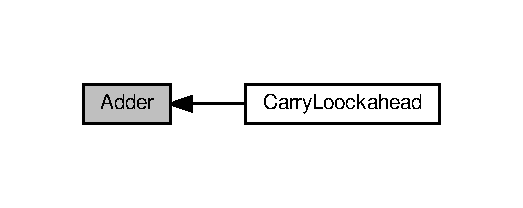
\includegraphics[width=251pt]{group___adder}
\end{center}
\end{figure}
\subsection*{Moduli}
\begin{DoxyCompactItemize}
\item 
\hyperlink{group___carry_loockahead}{Carry\+Loockahead}
\begin{DoxyCompactList}\small\item\em Addizionatore con carry-\/lookahead. \end{DoxyCompactList}\end{DoxyCompactItemize}
\subsection*{File}
\begin{DoxyCompactItemize}
\item 
file \hyperlink{cla__adder__cell_8vhd}{cla\+\_\+adder\+\_\+cell.\+vhd}
\end{DoxyCompactItemize}
\subsection*{Entities}
\begin{DoxyCompactItemize}
\item 
\hyperlink{classadder}{adder} entity
\item 
\hyperlink{classadder_1_1structural}{structural} architecture
\end{DoxyCompactItemize}
\subsection*{Components}
 \begin{DoxyCompactItemize}
\item 
\hyperlink{group___adder_gae7148956d4ef1d1cd14f35060634b9c3}{generic\+\_\+cla\+\_\+adder}  {\bfseries }  
\end{DoxyCompactItemize}
\subsection*{Generics}
 \begin{DoxyCompactItemize}
\item 
\hyperlink{group___adder_gae8451a648abadfad273ca1ae9b369657}{nbits} {\bfseries {\bfseries \textcolor{vhdlchar}{natural}\textcolor{vhdlchar}{ }\textcolor{vhdlchar}{ }\textcolor{vhdlchar}{\+:}\textcolor{vhdlchar}{=}\textcolor{vhdlchar}{ }\textcolor{vhdlchar}{ } \textcolor{vhdldigit}{8} \textcolor{vhdlchar}{ }}}
\item 
\hyperlink{group___adder_gadf05ca347ec6d3c85740dc697469b3db}{use\+\_\+custom} {\bfseries {\bfseries \textcolor{vhdlchar}{boolean}\textcolor{vhdlchar}{ }\textcolor{vhdlchar}{ }\textcolor{vhdlchar}{\+:}\textcolor{vhdlchar}{=}\textcolor{vhdlchar}{ }\textcolor{vhdlchar}{ }\textcolor{vhdlchar}{ }\textcolor{vhdlchar}{ }\textcolor{vhdlchar}{false}\textcolor{vhdlchar}{ }}}
\end{DoxyCompactItemize}
\subsection*{Ports}
 \begin{DoxyCompactItemize}
\item 
\hyperlink{group___adder_gad6ed6073f8ded668a403a0f7d85c53e8}{add1}  {\bfseries {\bfseries \textcolor{vhdlchar}{in}\textcolor{vhdlchar}{ }}} {\bfseries \textcolor{vhdlchar}{std\+\_\+logic\+\_\+vector}\textcolor{vhdlchar}{ }\textcolor{vhdlchar}{(}\textcolor{vhdlchar}{ }\textcolor{vhdlchar}{ }\textcolor{vhdlchar}{ }\textcolor{vhdlchar}{ }{\bfseries \hyperlink{group___adder_gae8451a648abadfad273ca1ae9b369657}{nbits}} \textcolor{vhdlchar}{-\/}\textcolor{vhdlchar}{ } \textcolor{vhdldigit}{1} \textcolor{vhdlchar}{ }\textcolor{vhdlchar}{downto}\textcolor{vhdlchar}{ }\textcolor{vhdlchar}{ } \textcolor{vhdldigit}{0} \textcolor{vhdlchar}{ }\textcolor{vhdlchar}{)}\textcolor{vhdlchar}{ }} 
\item 
\hyperlink{group___adder_gabf87ad241134c4d313c708910677575e}{add2}  {\bfseries {\bfseries \textcolor{vhdlchar}{in}\textcolor{vhdlchar}{ }}} {\bfseries \textcolor{vhdlchar}{std\+\_\+logic\+\_\+vector}\textcolor{vhdlchar}{ }\textcolor{vhdlchar}{(}\textcolor{vhdlchar}{ }\textcolor{vhdlchar}{ }\textcolor{vhdlchar}{ }\textcolor{vhdlchar}{ }{\bfseries \hyperlink{group___adder_gae8451a648abadfad273ca1ae9b369657}{nbits}} \textcolor{vhdlchar}{-\/}\textcolor{vhdlchar}{ } \textcolor{vhdldigit}{1} \textcolor{vhdlchar}{ }\textcolor{vhdlchar}{downto}\textcolor{vhdlchar}{ }\textcolor{vhdlchar}{ } \textcolor{vhdldigit}{0} \textcolor{vhdlchar}{ }\textcolor{vhdlchar}{)}\textcolor{vhdlchar}{ }} 
\item 
\hyperlink{group___adder_ga01f6ea3ddb4d1519676217bcb5959de8}{sum}  {\bfseries {\bfseries \textcolor{vhdlchar}{out}\textcolor{vhdlchar}{ }}} {\bfseries \textcolor{vhdlchar}{std\+\_\+logic\+\_\+vector}\textcolor{vhdlchar}{ }\textcolor{vhdlchar}{(}\textcolor{vhdlchar}{ }\textcolor{vhdlchar}{ }\textcolor{vhdlchar}{ }\textcolor{vhdlchar}{ }{\bfseries \hyperlink{group___adder_gae8451a648abadfad273ca1ae9b369657}{nbits}} \textcolor{vhdlchar}{-\/}\textcolor{vhdlchar}{ } \textcolor{vhdldigit}{1} \textcolor{vhdlchar}{ }\textcolor{vhdlchar}{downto}\textcolor{vhdlchar}{ }\textcolor{vhdlchar}{ } \textcolor{vhdldigit}{0} \textcolor{vhdlchar}{ }\textcolor{vhdlchar}{)}\textcolor{vhdlchar}{ }} 
\end{DoxyCompactItemize}


\subsection{Descrizione dettagliata}
Adder per la somma di due addendi con numero di bit variabile. 



\subsection{Documentazione delle variabili}
\hypertarget{group___adder_gad6ed6073f8ded668a403a0f7d85c53e8}{\index{Adder@{Adder}!add1@{add1}}
\index{add1@{add1}!Adder@{Adder}}
\subsubsection[{add1}]{\setlength{\rightskip}{0pt plus 5cm}{\bf add1} {\bfseries \textcolor{vhdlchar}{in}\textcolor{vhdlchar}{ }} {\bfseries \textcolor{vhdlchar}{std\+\_\+logic\+\_\+vector}\textcolor{vhdlchar}{ }\textcolor{vhdlchar}{(}\textcolor{vhdlchar}{ }\textcolor{vhdlchar}{ }\textcolor{vhdlchar}{ }\textcolor{vhdlchar}{ }{\bfseries {\bf nbits}} \textcolor{vhdlchar}{-\/}\textcolor{vhdlchar}{ } \textcolor{vhdldigit}{1} \textcolor{vhdlchar}{ }\textcolor{vhdlchar}{downto}\textcolor{vhdlchar}{ }\textcolor{vhdlchar}{ } \textcolor{vhdldigit}{0} \textcolor{vhdlchar}{ }\textcolor{vhdlchar}{)}\textcolor{vhdlchar}{ }} \hspace{0.3cm}{\ttfamily [Port]}}}\label{group___adder_gad6ed6073f8ded668a403a0f7d85c53e8}
\hypertarget{group___adder_gabf87ad241134c4d313c708910677575e}{\index{Adder@{Adder}!add2@{add2}}
\index{add2@{add2}!Adder@{Adder}}
\subsubsection[{add2}]{\setlength{\rightskip}{0pt plus 5cm}{\bf add2} {\bfseries \textcolor{vhdlchar}{in}\textcolor{vhdlchar}{ }} {\bfseries \textcolor{vhdlchar}{std\+\_\+logic\+\_\+vector}\textcolor{vhdlchar}{ }\textcolor{vhdlchar}{(}\textcolor{vhdlchar}{ }\textcolor{vhdlchar}{ }\textcolor{vhdlchar}{ }\textcolor{vhdlchar}{ }{\bfseries {\bf nbits}} \textcolor{vhdlchar}{-\/}\textcolor{vhdlchar}{ } \textcolor{vhdldigit}{1} \textcolor{vhdlchar}{ }\textcolor{vhdlchar}{downto}\textcolor{vhdlchar}{ }\textcolor{vhdlchar}{ } \textcolor{vhdldigit}{0} \textcolor{vhdlchar}{ }\textcolor{vhdlchar}{)}\textcolor{vhdlchar}{ }} \hspace{0.3cm}{\ttfamily [Port]}}}\label{group___adder_gabf87ad241134c4d313c708910677575e}
\hypertarget{group___adder_gae7148956d4ef1d1cd14f35060634b9c3}{\index{Adder@{Adder}!generic\+\_\+cla\+\_\+adder@{generic\+\_\+cla\+\_\+adder}}
\index{generic\+\_\+cla\+\_\+adder@{generic\+\_\+cla\+\_\+adder}!Adder@{Adder}}
\subsubsection[{generic\+\_\+cla\+\_\+adder}]{\setlength{\rightskip}{0pt plus 5cm}{\bf generic\+\_\+cla\+\_\+adder} {\bfseries \textcolor{vhdlchar}{ }} \hspace{0.3cm}{\ttfamily [Component]}}}\label{group___adder_gae7148956d4ef1d1cd14f35060634b9c3}
\hypertarget{group___adder_gae8451a648abadfad273ca1ae9b369657}{\index{Adder@{Adder}!nbits@{nbits}}
\index{nbits@{nbits}!Adder@{Adder}}
\subsubsection[{nbits}]{\setlength{\rightskip}{0pt plus 5cm}{\bf nbits} {\bfseries \textcolor{vhdlchar}{ }} {\bfseries \textcolor{vhdlchar}{natural}\textcolor{vhdlchar}{ }\textcolor{vhdlchar}{ }\textcolor{vhdlchar}{\+:}\textcolor{vhdlchar}{=}\textcolor{vhdlchar}{ }\textcolor{vhdlchar}{ } \textcolor{vhdldigit}{8} \textcolor{vhdlchar}{ }} \hspace{0.3cm}{\ttfamily [Generic]}}}\label{group___adder_gae8451a648abadfad273ca1ae9b369657}
\hypertarget{group___adder_ga01f6ea3ddb4d1519676217bcb5959de8}{\index{Adder@{Adder}!sum@{sum}}
\index{sum@{sum}!Adder@{Adder}}
\subsubsection[{sum}]{\setlength{\rightskip}{0pt plus 5cm}{\bf sum} {\bfseries \textcolor{vhdlchar}{out}\textcolor{vhdlchar}{ }} {\bfseries \textcolor{vhdlchar}{std\+\_\+logic\+\_\+vector}\textcolor{vhdlchar}{ }\textcolor{vhdlchar}{(}\textcolor{vhdlchar}{ }\textcolor{vhdlchar}{ }\textcolor{vhdlchar}{ }\textcolor{vhdlchar}{ }{\bfseries {\bf nbits}} \textcolor{vhdlchar}{-\/}\textcolor{vhdlchar}{ } \textcolor{vhdldigit}{1} \textcolor{vhdlchar}{ }\textcolor{vhdlchar}{downto}\textcolor{vhdlchar}{ }\textcolor{vhdlchar}{ } \textcolor{vhdldigit}{0} \textcolor{vhdlchar}{ }\textcolor{vhdlchar}{)}\textcolor{vhdlchar}{ }} \hspace{0.3cm}{\ttfamily [Port]}}}\label{group___adder_ga01f6ea3ddb4d1519676217bcb5959de8}
\hypertarget{group___adder_gadf05ca347ec6d3c85740dc697469b3db}{\index{Adder@{Adder}!use\+\_\+custom@{use\+\_\+custom}}
\index{use\+\_\+custom@{use\+\_\+custom}!Adder@{Adder}}
\subsubsection[{use\+\_\+custom}]{\setlength{\rightskip}{0pt plus 5cm}{\bf use\+\_\+custom} {\bfseries \textcolor{vhdlchar}{ }} {\bfseries \textcolor{vhdlchar}{boolean}\textcolor{vhdlchar}{ }\textcolor{vhdlchar}{ }\textcolor{vhdlchar}{\+:}\textcolor{vhdlchar}{=}\textcolor{vhdlchar}{ }\textcolor{vhdlchar}{ }\textcolor{vhdlchar}{ }\textcolor{vhdlchar}{ }\textcolor{vhdlchar}{false}\textcolor{vhdlchar}{ }} \hspace{0.3cm}{\ttfamily [Generic]}}}\label{group___adder_gadf05ca347ec6d3c85740dc697469b3db}

\hypertarget{group___carry_loockahead}{}\section{Carry\+Loockahead}
\label{group___carry_loockahead}\index{Carry\+Loockahead@{Carry\+Loockahead}}


Addizionatore con carry-\/lookahead.  


Diagramma di collaborazione per Carry\+Loockahead\+:\nopagebreak
\begin{figure}[H]
\begin{center}
\leavevmode
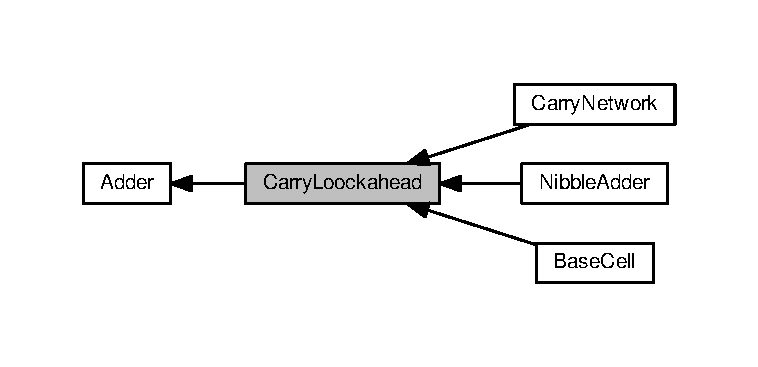
\includegraphics[width=350pt]{group___carry_loockahead}
\end{center}
\end{figure}
\subsection*{Moduli}
\begin{DoxyCompactItemize}
\item 
\hyperlink{group___base_cell}{Base\+Cell}
\begin{DoxyCompactList}\small\item\em Implementazione della cella base di un adder. \end{DoxyCompactList}\item 
\hyperlink{group___carry_network}{Carry\+Network}
\begin{DoxyCompactList}\small\item\em Rete di generazione dei segnali di carry per un adder a quattro bit. \end{DoxyCompactList}\item 
\hyperlink{group___nibble_adder}{Nibble\+Adder}
\begin{DoxyCompactList}\small\item\em Blocco elementare di somma a quattro bit. \end{DoxyCompactList}\end{DoxyCompactItemize}
\subsection*{Entities}
\begin{DoxyCompactItemize}
\item 
\hyperlink{classgeneric__cla__adder}{generic\+\_\+cla\+\_\+adder} entity
\begin{DoxyCompactList}\small\item\em Adder custom con carry-\/lookahead

\hyperlink{classgeneric__cla__adder}{generic\+\_\+cla\+\_\+adder} somma tra loro due addendi ed un carry in ingresso; gli addendi sono espressi su multipli interi di quattro bit. Oltre a generare la somma, genera il flag di carry ed il flag di overflow. \end{DoxyCompactList}\item 
\hyperlink{classgeneric__cla__adder_1_1structural}{structural} architecture
\begin{DoxyCompactList}\small\item\em Implementazione structural di \hyperlink{classgeneric__cla__adder}{generic\+\_\+cla\+\_\+adder}.

Questa implementazione istanzia tanti blocchi \hyperlink{classnibble__adder}{nibble\+\_\+adder} quanti siano i nibble in cui sono rappresentati gli addendi. La somma è espressa sullo stesso numero di bit. I diversi blocchi sono connessi tra loro come indicato nello schema ricordato di seguito\+: . \end{DoxyCompactList}\end{DoxyCompactItemize}
\subsection*{Components}
 \begin{DoxyCompactItemize}
\item 
\hyperlink{group___carry_loockahead_ga98a3a5b152caf0f2de1e31ac60088369}{nibble\+\_\+adder}  {\bfseries }  
\end{DoxyCompactItemize}
\subsection*{Generics}
 \begin{DoxyCompactItemize}
\item 
\hyperlink{group___carry_loockahead_ga0b63b586531492d0fa882246cca071c1}{nibbles} {\bfseries {\bfseries \textcolor{vhdlchar}{natural}\textcolor{vhdlchar}{ }\textcolor{vhdlchar}{ }\textcolor{vhdlchar}{\+:}\textcolor{vhdlchar}{=}\textcolor{vhdlchar}{ }\textcolor{vhdlchar}{ } \textcolor{vhdldigit}{2} \textcolor{vhdlchar}{ }}}
\end{DoxyCompactItemize}
\subsection*{Ports}
 \begin{DoxyCompactItemize}
\item 
\hyperlink{group___carry_loockahead_ga1c211cdf2d4cf97e869c442832c53439}{carry\+\_\+in}  {\bfseries {\bfseries \textcolor{vhdlchar}{in}\textcolor{vhdlchar}{ }}} {\bfseries \textcolor{vhdlchar}{std\+\_\+logic}\textcolor{vhdlchar}{ }} 
\item 
\hyperlink{group___carry_loockahead_gae4a2e124144a2f35270a55f0cf32a5ee}{addendum1}  {\bfseries {\bfseries \textcolor{vhdlchar}{in}\textcolor{vhdlchar}{ }}} {\bfseries \textcolor{vhdlchar}{std\+\_\+logic\+\_\+vector}\textcolor{vhdlchar}{ }\textcolor{vhdlchar}{(}\textcolor{vhdlchar}{ }\textcolor{vhdlchar}{(}\textcolor{vhdlchar}{ }\textcolor{vhdlchar}{ }\textcolor{vhdlchar}{ }\textcolor{vhdlchar}{ }{\bfseries \hyperlink{group___carry_loockahead_ga0b63b586531492d0fa882246cca071c1}{nibbles}} \textcolor{vhdlchar}{$\ast$}\textcolor{vhdlchar}{ } \textcolor{vhdldigit}{4} \textcolor{vhdlchar}{ }\textcolor{vhdlchar}{)}\textcolor{vhdlchar}{ }\textcolor{vhdlchar}{-\/}\textcolor{vhdlchar}{ } \textcolor{vhdldigit}{1} \textcolor{vhdlchar}{ }\textcolor{vhdlchar}{downto}\textcolor{vhdlchar}{ }\textcolor{vhdlchar}{ } \textcolor{vhdldigit}{0} \textcolor{vhdlchar}{ }\textcolor{vhdlchar}{)}\textcolor{vhdlchar}{ }} 
\begin{DoxyCompactList}\small\item\em addendo 1, espresso in complemento a due \end{DoxyCompactList}\item 
\hyperlink{group___carry_loockahead_ga2715463c615cf8418f85c6a1427ce62c}{addendum2}  {\bfseries {\bfseries \textcolor{vhdlchar}{in}\textcolor{vhdlchar}{ }}} {\bfseries \textcolor{vhdlchar}{std\+\_\+logic\+\_\+vector}\textcolor{vhdlchar}{ }\textcolor{vhdlchar}{(}\textcolor{vhdlchar}{ }\textcolor{vhdlchar}{(}\textcolor{vhdlchar}{ }\textcolor{vhdlchar}{ }\textcolor{vhdlchar}{ }\textcolor{vhdlchar}{ }{\bfseries \hyperlink{group___carry_loockahead_ga0b63b586531492d0fa882246cca071c1}{nibbles}} \textcolor{vhdlchar}{$\ast$}\textcolor{vhdlchar}{ } \textcolor{vhdldigit}{4} \textcolor{vhdlchar}{ }\textcolor{vhdlchar}{)}\textcolor{vhdlchar}{ }\textcolor{vhdlchar}{-\/}\textcolor{vhdlchar}{ } \textcolor{vhdldigit}{1} \textcolor{vhdlchar}{ }\textcolor{vhdlchar}{downto}\textcolor{vhdlchar}{ }\textcolor{vhdlchar}{ } \textcolor{vhdldigit}{0} \textcolor{vhdlchar}{ }\textcolor{vhdlchar}{)}\textcolor{vhdlchar}{ }} 
\begin{DoxyCompactList}\small\item\em addendo 2, espresso in complemento a due \end{DoxyCompactList}\item 
\hyperlink{group___carry_loockahead_ga1b4798a9e96bb32e9c08ce68e24e7871}{sum}  {\bfseries {\bfseries \textcolor{vhdlchar}{out}\textcolor{vhdlchar}{ }}} {\bfseries \textcolor{vhdlchar}{std\+\_\+logic\+\_\+vector}\textcolor{vhdlchar}{ }\textcolor{vhdlchar}{(}\textcolor{vhdlchar}{ }\textcolor{vhdlchar}{(}\textcolor{vhdlchar}{ }\textcolor{vhdlchar}{ }\textcolor{vhdlchar}{ }\textcolor{vhdlchar}{ }{\bfseries \hyperlink{group___carry_loockahead_ga0b63b586531492d0fa882246cca071c1}{nibbles}} \textcolor{vhdlchar}{$\ast$}\textcolor{vhdlchar}{ } \textcolor{vhdldigit}{4} \textcolor{vhdlchar}{ }\textcolor{vhdlchar}{)}\textcolor{vhdlchar}{ }\textcolor{vhdlchar}{-\/}\textcolor{vhdlchar}{ } \textcolor{vhdldigit}{1} \textcolor{vhdlchar}{ }\textcolor{vhdlchar}{downto}\textcolor{vhdlchar}{ }\textcolor{vhdlchar}{ } \textcolor{vhdldigit}{0} \textcolor{vhdlchar}{ }\textcolor{vhdlchar}{)}\textcolor{vhdlchar}{ }} 
\begin{DoxyCompactList}\small\item\em somma degli addendi, espressa in complemento a due \end{DoxyCompactList}\item 
\hyperlink{group___carry_loockahead_ga851aaea297bdc862fba5478c4bf0e214}{carry\+\_\+out}  {\bfseries {\bfseries \textcolor{vhdlchar}{out}\textcolor{vhdlchar}{ }}} {\bfseries \textcolor{vhdlchar}{std\+\_\+logic}\textcolor{vhdlchar}{ }} 
\item 
\hyperlink{group___carry_loockahead_ga9650307dde287e0bcfa1e26370c006c2}{overflow}  {\bfseries {\bfseries \textcolor{vhdlchar}{out}\textcolor{vhdlchar}{ }}} {\bfseries \textcolor{vhdlchar}{std\+\_\+logic}\textcolor{vhdlchar}{ }} 
\end{DoxyCompactItemize}
\subsection*{Signals}
 \begin{DoxyCompactItemize}
\item 
\hyperlink{group___carry_loockahead_ga19afe0b89973d7fc29362431f2e828b7}{prop} {\bfseries \textcolor{vhdlchar}{std\+\_\+logic\+\_\+vector}\textcolor{vhdlchar}{ }\textcolor{vhdlchar}{(}\textcolor{vhdlchar}{ }\textcolor{vhdlchar}{ } \textcolor{vhdldigit}{0} \textcolor{vhdlchar}{ }\textcolor{vhdlchar}{to}\textcolor{vhdlchar}{ }\textcolor{vhdlchar}{ }\textcolor{vhdlchar}{ }\textcolor{vhdlchar}{ }{\bfseries \hyperlink{group___carry_loockahead_ga0b63b586531492d0fa882246cca071c1}{nibbles}} \textcolor{vhdlchar}{ }\textcolor{vhdlchar}{)}\textcolor{vhdlchar}{ }} 
\item 
\hyperlink{group___carry_loockahead_ga7a68948b7b96c7b51036939fad8e71b3}{gen} {\bfseries \textcolor{vhdlchar}{std\+\_\+logic\+\_\+vector}\textcolor{vhdlchar}{ }\textcolor{vhdlchar}{(}\textcolor{vhdlchar}{ }\textcolor{vhdlchar}{ } \textcolor{vhdldigit}{0} \textcolor{vhdlchar}{ }\textcolor{vhdlchar}{to}\textcolor{vhdlchar}{ }\textcolor{vhdlchar}{ }\textcolor{vhdlchar}{ }\textcolor{vhdlchar}{ }{\bfseries \hyperlink{group___carry_loockahead_ga0b63b586531492d0fa882246cca071c1}{nibbles}} \textcolor{vhdlchar}{ }\textcolor{vhdlchar}{)}\textcolor{vhdlchar}{ }} 
\item 
\hyperlink{group___carry_loockahead_ga3c7f619aa6449e06bf0dd48a7db92b84}{sum\+\_\+tmp} {\bfseries \textcolor{vhdlchar}{std\+\_\+logic\+\_\+vector}\textcolor{vhdlchar}{ }\textcolor{vhdlchar}{(}\textcolor{vhdlchar}{ }\textcolor{vhdlchar}{(}\textcolor{vhdlchar}{ }\textcolor{vhdlchar}{ }\textcolor{vhdlchar}{ }\textcolor{vhdlchar}{ }{\bfseries \hyperlink{group___carry_loockahead_ga0b63b586531492d0fa882246cca071c1}{nibbles}} \textcolor{vhdlchar}{$\ast$}\textcolor{vhdlchar}{ } \textcolor{vhdldigit}{4} \textcolor{vhdlchar}{ }\textcolor{vhdlchar}{)}\textcolor{vhdlchar}{ }\textcolor{vhdlchar}{-\/}\textcolor{vhdlchar}{ } \textcolor{vhdldigit}{1} \textcolor{vhdlchar}{ }\textcolor{vhdlchar}{downto}\textcolor{vhdlchar}{ }\textcolor{vhdlchar}{ } \textcolor{vhdldigit}{0} \textcolor{vhdlchar}{ }\textcolor{vhdlchar}{)}\textcolor{vhdlchar}{ }} 
\end{DoxyCompactItemize}


\subsection{Descrizione dettagliata}
Addizionatore con carry-\/lookahead. 



\subsection{Documentazione delle variabili}
\index{Carry\+Loockahead@{Carry\+Loockahead}!addendum1@{addendum1}}
\index{addendum1@{addendum1}!Carry\+Loockahead@{Carry\+Loockahead}}
\subsubsection[{\texorpdfstring{addendum1}{addendum1}}]{\setlength{\rightskip}{0pt plus 5cm}{\bf addendum1} {\bfseries \textcolor{vhdlchar}{in}\textcolor{vhdlchar}{ }} {\bfseries \textcolor{vhdlchar}{std\+\_\+logic\+\_\+vector}\textcolor{vhdlchar}{ }\textcolor{vhdlchar}{(}\textcolor{vhdlchar}{ }\textcolor{vhdlchar}{(}\textcolor{vhdlchar}{ }\textcolor{vhdlchar}{ }\textcolor{vhdlchar}{ }\textcolor{vhdlchar}{ }{\bfseries {\bf nibbles}} \textcolor{vhdlchar}{$\ast$}\textcolor{vhdlchar}{ } \textcolor{vhdldigit}{4} \textcolor{vhdlchar}{ }\textcolor{vhdlchar}{)}\textcolor{vhdlchar}{ }\textcolor{vhdlchar}{-\/}\textcolor{vhdlchar}{ } \textcolor{vhdldigit}{1} \textcolor{vhdlchar}{ }\textcolor{vhdlchar}{downto}\textcolor{vhdlchar}{ }\textcolor{vhdlchar}{ } \textcolor{vhdldigit}{0} \textcolor{vhdlchar}{ }\textcolor{vhdlchar}{)}\textcolor{vhdlchar}{ }} \hspace{0.3cm}{\ttfamily [Port]}}\hypertarget{group___carry_loockahead_gae4a2e124144a2f35270a55f0cf32a5ee}{}\label{group___carry_loockahead_gae4a2e124144a2f35270a55f0cf32a5ee}


addendo 1, espresso in complemento a due 

segnale di \char`\"{}carry-\/in\char`\"{}, prodotto da un eventuale \hyperlink{classnibble__adder}{nibble\+\_\+adder} a monte; Può essere posto a \textquotesingle{}0\textquotesingle{} nel caso in cui non vi siano adder a monte. \index{Carry\+Loockahead@{Carry\+Loockahead}!addendum2@{addendum2}}
\index{addendum2@{addendum2}!Carry\+Loockahead@{Carry\+Loockahead}}
\subsubsection[{\texorpdfstring{addendum2}{addendum2}}]{\setlength{\rightskip}{0pt plus 5cm}{\bf addendum2} {\bfseries \textcolor{vhdlchar}{in}\textcolor{vhdlchar}{ }} {\bfseries \textcolor{vhdlchar}{std\+\_\+logic\+\_\+vector}\textcolor{vhdlchar}{ }\textcolor{vhdlchar}{(}\textcolor{vhdlchar}{ }\textcolor{vhdlchar}{(}\textcolor{vhdlchar}{ }\textcolor{vhdlchar}{ }\textcolor{vhdlchar}{ }\textcolor{vhdlchar}{ }{\bfseries {\bf nibbles}} \textcolor{vhdlchar}{$\ast$}\textcolor{vhdlchar}{ } \textcolor{vhdldigit}{4} \textcolor{vhdlchar}{ }\textcolor{vhdlchar}{)}\textcolor{vhdlchar}{ }\textcolor{vhdlchar}{-\/}\textcolor{vhdlchar}{ } \textcolor{vhdldigit}{1} \textcolor{vhdlchar}{ }\textcolor{vhdlchar}{downto}\textcolor{vhdlchar}{ }\textcolor{vhdlchar}{ } \textcolor{vhdldigit}{0} \textcolor{vhdlchar}{ }\textcolor{vhdlchar}{)}\textcolor{vhdlchar}{ }} \hspace{0.3cm}{\ttfamily [Port]}}\hypertarget{group___carry_loockahead_ga2715463c615cf8418f85c6a1427ce62c}{}\label{group___carry_loockahead_ga2715463c615cf8418f85c6a1427ce62c}


addendo 2, espresso in complemento a due 

\index{Carry\+Loockahead@{Carry\+Loockahead}!carry\+\_\+in@{carry\+\_\+in}}
\index{carry\+\_\+in@{carry\+\_\+in}!Carry\+Loockahead@{Carry\+Loockahead}}
\subsubsection[{\texorpdfstring{carry\+\_\+in}{carry_in}}]{\setlength{\rightskip}{0pt plus 5cm}{\bf carry\+\_\+in} {\bfseries \textcolor{vhdlchar}{in}\textcolor{vhdlchar}{ }} {\bfseries \textcolor{vhdlchar}{std\+\_\+logic}\textcolor{vhdlchar}{ }} \hspace{0.3cm}{\ttfamily [Port]}}\hypertarget{group___carry_loockahead_ga1c211cdf2d4cf97e869c442832c53439}{}\label{group___carry_loockahead_ga1c211cdf2d4cf97e869c442832c53439}
numero di nibble in cui sono rappresentati gli addendi e nel quale sarà espressa la somma degli stessi \index{Carry\+Loockahead@{Carry\+Loockahead}!carry\+\_\+out@{carry\+\_\+out}}
\index{carry\+\_\+out@{carry\+\_\+out}!Carry\+Loockahead@{Carry\+Loockahead}}
\subsubsection[{\texorpdfstring{carry\+\_\+out}{carry_out}}]{\setlength{\rightskip}{0pt plus 5cm}{\bf carry\+\_\+out} {\bfseries \textcolor{vhdlchar}{out}\textcolor{vhdlchar}{ }} {\bfseries \textcolor{vhdlchar}{std\+\_\+logic}\textcolor{vhdlchar}{ }} \hspace{0.3cm}{\ttfamily [Port]}}\hypertarget{group___carry_loockahead_ga851aaea297bdc862fba5478c4bf0e214}{}\label{group___carry_loockahead_ga851aaea297bdc862fba5478c4bf0e214}
\index{Carry\+Loockahead@{Carry\+Loockahead}!gen@{gen}}
\index{gen@{gen}!Carry\+Loockahead@{Carry\+Loockahead}}
\subsubsection[{\texorpdfstring{gen}{gen}}]{\setlength{\rightskip}{0pt plus 5cm}{\bf gen} {\bfseries \textcolor{vhdlchar}{std\+\_\+logic\+\_\+vector}\textcolor{vhdlchar}{ }\textcolor{vhdlchar}{(}\textcolor{vhdlchar}{ }\textcolor{vhdlchar}{ } \textcolor{vhdldigit}{0} \textcolor{vhdlchar}{ }\textcolor{vhdlchar}{to}\textcolor{vhdlchar}{ }\textcolor{vhdlchar}{ }\textcolor{vhdlchar}{ }\textcolor{vhdlchar}{ }{\bfseries {\bf nibbles}} \textcolor{vhdlchar}{ }\textcolor{vhdlchar}{)}\textcolor{vhdlchar}{ }} \hspace{0.3cm}{\ttfamily [Signal]}}\hypertarget{group___carry_loockahead_ga7a68948b7b96c7b51036939fad8e71b3}{}\label{group___carry_loockahead_ga7a68948b7b96c7b51036939fad8e71b3}
funzione \char`\"{}propagazione\char`\"{} del carry, prodotta dai diversi blocchi \hyperlink{classnibble__adder}{nibble\+\_\+adder}; prop(i) vale 1 quando, sulla base degli ingressi, l\textquotesingle{}i-\/esimo \hyperlink{classnibble__adder}{nibble\+\_\+adder} propaghera\textquotesingle{} un eventuale carry in ingresso; prop(0) = \textquotesingle{}1\textquotesingle{}; \index{Carry\+Loockahead@{Carry\+Loockahead}!nibble\+\_\+adder@{nibble\+\_\+adder}}
\index{nibble\+\_\+adder@{nibble\+\_\+adder}!Carry\+Loockahead@{Carry\+Loockahead}}
\subsubsection[{\texorpdfstring{nibble\+\_\+adder}{nibble_adder}}]{\setlength{\rightskip}{0pt plus 5cm}{\bf nibble\+\_\+adder} {\bfseries \textcolor{vhdlchar}{ }} \hspace{0.3cm}{\ttfamily [Component]}}\hypertarget{group___carry_loockahead_ga98a3a5b152caf0f2de1e31ac60088369}{}\label{group___carry_loockahead_ga98a3a5b152caf0f2de1e31ac60088369}
\index{Carry\+Loockahead@{Carry\+Loockahead}!nibbles@{nibbles}}
\index{nibbles@{nibbles}!Carry\+Loockahead@{Carry\+Loockahead}}
\subsubsection[{\texorpdfstring{nibbles}{nibbles}}]{\setlength{\rightskip}{0pt plus 5cm}{\bf nibbles} {\bfseries \textcolor{vhdlchar}{ }} {\bfseries \textcolor{vhdlchar}{natural}\textcolor{vhdlchar}{ }\textcolor{vhdlchar}{ }\textcolor{vhdlchar}{\+:}\textcolor{vhdlchar}{=}\textcolor{vhdlchar}{ }\textcolor{vhdlchar}{ } \textcolor{vhdldigit}{2} \textcolor{vhdlchar}{ }} \hspace{0.3cm}{\ttfamily [Generic]}}\hypertarget{group___carry_loockahead_ga0b63b586531492d0fa882246cca071c1}{}\label{group___carry_loockahead_ga0b63b586531492d0fa882246cca071c1}
\index{Carry\+Loockahead@{Carry\+Loockahead}!overflow@{overflow}}
\index{overflow@{overflow}!Carry\+Loockahead@{Carry\+Loockahead}}
\subsubsection[{\texorpdfstring{overflow}{overflow}}]{\setlength{\rightskip}{0pt plus 5cm}{\bf overflow} {\bfseries \textcolor{vhdlchar}{out}\textcolor{vhdlchar}{ }} {\bfseries \textcolor{vhdlchar}{std\+\_\+logic}\textcolor{vhdlchar}{ }} \hspace{0.3cm}{\ttfamily [Port]}}\hypertarget{group___carry_loockahead_ga9650307dde287e0bcfa1e26370c006c2}{}\label{group___carry_loockahead_ga9650307dde287e0bcfa1e26370c006c2}
carry in uscita; viene calcolato come carry\+\_\+out=gen(nibbles)+(prop(nibbles)$\ast$carry\+\_\+in), dove gen(nibbles) e prop(nibbles) sono, rispettivamente, la funzione \char`\"{}generazione\char`\"{} e \char`\"{}propagazione\char`\"{} del carry prodotta dall\textquotesingle{}ultimo blocco \hyperlink{classnibble__adder}{nibble\+\_\+adder}, cioè quello che somma i nibble di peso massimo, e carry\+\_\+in e\textquotesingle{} il carry in ingresso al sommatore. \index{Carry\+Loockahead@{Carry\+Loockahead}!prop@{prop}}
\index{prop@{prop}!Carry\+Loockahead@{Carry\+Loockahead}}
\subsubsection[{\texorpdfstring{prop}{prop}}]{\setlength{\rightskip}{0pt plus 5cm}{\bf prop} {\bfseries \textcolor{vhdlchar}{std\+\_\+logic\+\_\+vector}\textcolor{vhdlchar}{ }\textcolor{vhdlchar}{(}\textcolor{vhdlchar}{ }\textcolor{vhdlchar}{ } \textcolor{vhdldigit}{0} \textcolor{vhdlchar}{ }\textcolor{vhdlchar}{to}\textcolor{vhdlchar}{ }\textcolor{vhdlchar}{ }\textcolor{vhdlchar}{ }\textcolor{vhdlchar}{ }{\bfseries {\bf nibbles}} \textcolor{vhdlchar}{ }\textcolor{vhdlchar}{)}\textcolor{vhdlchar}{ }} \hspace{0.3cm}{\ttfamily [Signal]}}\hypertarget{group___carry_loockahead_ga19afe0b89973d7fc29362431f2e828b7}{}\label{group___carry_loockahead_ga19afe0b89973d7fc29362431f2e828b7}
\index{Carry\+Loockahead@{Carry\+Loockahead}!sum@{sum}}
\index{sum@{sum}!Carry\+Loockahead@{Carry\+Loockahead}}
\subsubsection[{\texorpdfstring{sum}{sum}}]{\setlength{\rightskip}{0pt plus 5cm}{\bf sum} {\bfseries \textcolor{vhdlchar}{out}\textcolor{vhdlchar}{ }} {\bfseries \textcolor{vhdlchar}{std\+\_\+logic\+\_\+vector}\textcolor{vhdlchar}{ }\textcolor{vhdlchar}{(}\textcolor{vhdlchar}{ }\textcolor{vhdlchar}{(}\textcolor{vhdlchar}{ }\textcolor{vhdlchar}{ }\textcolor{vhdlchar}{ }\textcolor{vhdlchar}{ }{\bfseries {\bf nibbles}} \textcolor{vhdlchar}{$\ast$}\textcolor{vhdlchar}{ } \textcolor{vhdldigit}{4} \textcolor{vhdlchar}{ }\textcolor{vhdlchar}{)}\textcolor{vhdlchar}{ }\textcolor{vhdlchar}{-\/}\textcolor{vhdlchar}{ } \textcolor{vhdldigit}{1} \textcolor{vhdlchar}{ }\textcolor{vhdlchar}{downto}\textcolor{vhdlchar}{ }\textcolor{vhdlchar}{ } \textcolor{vhdldigit}{0} \textcolor{vhdlchar}{ }\textcolor{vhdlchar}{)}\textcolor{vhdlchar}{ }} \hspace{0.3cm}{\ttfamily [Port]}}\hypertarget{group___carry_loockahead_ga1b4798a9e96bb32e9c08ce68e24e7871}{}\label{group___carry_loockahead_ga1b4798a9e96bb32e9c08ce68e24e7871}


somma degli addendi, espressa in complemento a due 

\index{Carry\+Loockahead@{Carry\+Loockahead}!sum\+\_\+tmp@{sum\+\_\+tmp}}
\index{sum\+\_\+tmp@{sum\+\_\+tmp}!Carry\+Loockahead@{Carry\+Loockahead}}
\subsubsection[{\texorpdfstring{sum\+\_\+tmp}{sum_tmp}}]{\setlength{\rightskip}{0pt plus 5cm}{\bf sum\+\_\+tmp} {\bfseries \textcolor{vhdlchar}{std\+\_\+logic\+\_\+vector}\textcolor{vhdlchar}{ }\textcolor{vhdlchar}{(}\textcolor{vhdlchar}{ }\textcolor{vhdlchar}{(}\textcolor{vhdlchar}{ }\textcolor{vhdlchar}{ }\textcolor{vhdlchar}{ }\textcolor{vhdlchar}{ }{\bfseries {\bf nibbles}} \textcolor{vhdlchar}{$\ast$}\textcolor{vhdlchar}{ } \textcolor{vhdldigit}{4} \textcolor{vhdlchar}{ }\textcolor{vhdlchar}{)}\textcolor{vhdlchar}{ }\textcolor{vhdlchar}{-\/}\textcolor{vhdlchar}{ } \textcolor{vhdldigit}{1} \textcolor{vhdlchar}{ }\textcolor{vhdlchar}{downto}\textcolor{vhdlchar}{ }\textcolor{vhdlchar}{ } \textcolor{vhdldigit}{0} \textcolor{vhdlchar}{ }\textcolor{vhdlchar}{)}\textcolor{vhdlchar}{ }} \hspace{0.3cm}{\ttfamily [Signal]}}\hypertarget{group___carry_loockahead_ga3c7f619aa6449e06bf0dd48a7db92b84}{}\label{group___carry_loockahead_ga3c7f619aa6449e06bf0dd48a7db92b84}
funzione \char`\"{}generazione\char`\"{} del carry, prodotta dai diversi blocchi \hyperlink{classnibble__adder}{nibble\+\_\+adder}; gen(i) vale 1 quando, sulla base degli ingressi, l\textquotesingle{}i-\/esimo \hyperlink{classnibble__adder}{nibble\+\_\+adder} genera carry in uscita; gen(0) = \textquotesingle{}0\textquotesingle{}; 
\hypertarget{group___base_cell}{}\section{Base\+Cell}
\label{group___base_cell}\index{Base\+Cell@{Base\+Cell}}


Implementazione della cella base di un adder.  


Diagramma di collaborazione per Base\+Cell\+:\nopagebreak
\begin{figure}[H]
\begin{center}
\leavevmode
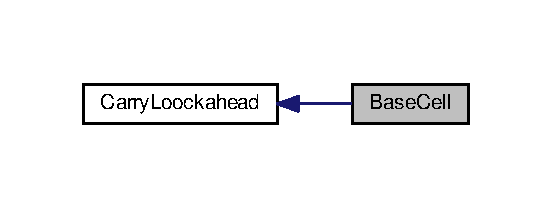
\includegraphics[width=265pt]{group___base_cell}
\end{center}
\end{figure}
\subsection*{Entities}
\begin{DoxyCompactItemize}
\item 
\hyperlink{classcla__adder__cell}{cla\+\_\+adder\+\_\+cell} entity
\begin{DoxyCompactList}\small\item\em Cella base di un addizionatore con carry-\/lookahead.

La cella somma tra loro due addendi ed un carry in ingresso, tutti espressi su un solo bit. Oltre a generare la somma, genera le funzioni \char`\"{}propagazione\char`\"{} e \char`\"{}generazione\char`\"{} del carry. \end{DoxyCompactList}\item 
\hyperlink{classcla__adder__cell_1_1dataflow}{dataflow} architecture
\end{DoxyCompactItemize}
\subsection*{Ports}
 \begin{DoxyCompactItemize}
\item 
\hyperlink{group___base_cell_ga2b16ee1ce0d8ffb8f85ccea13f8ba38d}{add1}  {\bfseries {\bfseries \textcolor{vhdlchar}{in}\textcolor{vhdlchar}{ }}} {\bfseries \textcolor{vhdlchar}{std\+\_\+logic}\textcolor{vhdlchar}{ }} 
\begin{DoxyCompactList}\small\item\em addendo 1 \end{DoxyCompactList}\item 
\hyperlink{group___base_cell_gac3ebb689e34fc5e7657726b18d8b5369}{add2}  {\bfseries {\bfseries \textcolor{vhdlchar}{in}\textcolor{vhdlchar}{ }}} {\bfseries \textcolor{vhdlchar}{std\+\_\+logic}\textcolor{vhdlchar}{ }} 
\begin{DoxyCompactList}\small\item\em addendo 2 \end{DoxyCompactList}\item 
\hyperlink{group___base_cell_gaa556a73dc4a4de1a0d662b25adbcbe33}{carryin}  {\bfseries {\bfseries \textcolor{vhdlchar}{in}\textcolor{vhdlchar}{ }}} {\bfseries \textcolor{vhdlchar}{std\+\_\+logic}\textcolor{vhdlchar}{ }} 
\begin{DoxyCompactList}\small\item\em carry in ingresso \end{DoxyCompactList}\item 
\hyperlink{group___base_cell_gac94466f3a0e3e34f0231abcf4b667ade}{prop}  {\bfseries {\bfseries \textcolor{vhdlchar}{out}\textcolor{vhdlchar}{ }}} {\bfseries \textcolor{vhdlchar}{std\+\_\+logic}\textcolor{vhdlchar}{ }} 
\item 
\hyperlink{group___base_cell_gaad65a9c9ebd4dd83c2835249a1ba2dff}{gen}  {\bfseries {\bfseries \textcolor{vhdlchar}{out}\textcolor{vhdlchar}{ }}} {\bfseries \textcolor{vhdlchar}{std\+\_\+logic}\textcolor{vhdlchar}{ }} 
\item 
\hyperlink{group___base_cell_ga0d9fc1b21b42422b12d68ad73ca8ef13}{sum}  {\bfseries {\bfseries \textcolor{vhdlchar}{out}\textcolor{vhdlchar}{ }}} {\bfseries \textcolor{vhdlchar}{std\+\_\+logic}\textcolor{vhdlchar}{ }} 
\end{DoxyCompactItemize}


\subsection{Descrizione dettagliata}
Implementazione della cella base di un adder. 



\subsection{Documentazione delle variabili}
\index{Base\+Cell@{Base\+Cell}!add1@{add1}}
\index{add1@{add1}!Base\+Cell@{Base\+Cell}}
\subsubsection[{\texorpdfstring{add1}{add1}}]{\setlength{\rightskip}{0pt plus 5cm}{\bf add1} {\bfseries \textcolor{vhdlchar}{in}\textcolor{vhdlchar}{ }} {\bfseries \textcolor{vhdlchar}{std\+\_\+logic}\textcolor{vhdlchar}{ }} \hspace{0.3cm}{\ttfamily [Port]}}\hypertarget{group___base_cell_ga2b16ee1ce0d8ffb8f85ccea13f8ba38d}{}\label{group___base_cell_ga2b16ee1ce0d8ffb8f85ccea13f8ba38d}


addendo 1 

\index{Base\+Cell@{Base\+Cell}!add2@{add2}}
\index{add2@{add2}!Base\+Cell@{Base\+Cell}}
\subsubsection[{\texorpdfstring{add2}{add2}}]{\setlength{\rightskip}{0pt plus 5cm}{\bf add2} {\bfseries \textcolor{vhdlchar}{in}\textcolor{vhdlchar}{ }} {\bfseries \textcolor{vhdlchar}{std\+\_\+logic}\textcolor{vhdlchar}{ }} \hspace{0.3cm}{\ttfamily [Port]}}\hypertarget{group___base_cell_gac3ebb689e34fc5e7657726b18d8b5369}{}\label{group___base_cell_gac3ebb689e34fc5e7657726b18d8b5369}


addendo 2 

\index{Base\+Cell@{Base\+Cell}!carryin@{carryin}}
\index{carryin@{carryin}!Base\+Cell@{Base\+Cell}}
\subsubsection[{\texorpdfstring{carryin}{carryin}}]{\setlength{\rightskip}{0pt plus 5cm}{\bf carryin} {\bfseries \textcolor{vhdlchar}{in}\textcolor{vhdlchar}{ }} {\bfseries \textcolor{vhdlchar}{std\+\_\+logic}\textcolor{vhdlchar}{ }} \hspace{0.3cm}{\ttfamily [Port]}}\hypertarget{group___base_cell_gaa556a73dc4a4de1a0d662b25adbcbe33}{}\label{group___base_cell_gaa556a73dc4a4de1a0d662b25adbcbe33}


carry in ingresso 

\index{Base\+Cell@{Base\+Cell}!gen@{gen}}
\index{gen@{gen}!Base\+Cell@{Base\+Cell}}
\subsubsection[{\texorpdfstring{gen}{gen}}]{\setlength{\rightskip}{0pt plus 5cm}{\bf gen} {\bfseries \textcolor{vhdlchar}{out}\textcolor{vhdlchar}{ }} {\bfseries \textcolor{vhdlchar}{std\+\_\+logic}\textcolor{vhdlchar}{ }} \hspace{0.3cm}{\ttfamily [Port]}}\hypertarget{group___base_cell_gaad65a9c9ebd4dd83c2835249a1ba2dff}{}\label{group___base_cell_gaad65a9c9ebd4dd83c2835249a1ba2dff}
funzione "propagazione”, vale 1 quando, sulla base degli ingressi, un adder propaghera\textquotesingle{} un eventuale carry in ingresso; prop = add1 OR add2 \index{Base\+Cell@{Base\+Cell}!prop@{prop}}
\index{prop@{prop}!Base\+Cell@{Base\+Cell}}
\subsubsection[{\texorpdfstring{prop}{prop}}]{\setlength{\rightskip}{0pt plus 5cm}{\bf prop} {\bfseries \textcolor{vhdlchar}{out}\textcolor{vhdlchar}{ }} {\bfseries \textcolor{vhdlchar}{std\+\_\+logic}\textcolor{vhdlchar}{ }} \hspace{0.3cm}{\ttfamily [Port]}}\hypertarget{group___base_cell_gac94466f3a0e3e34f0231abcf4b667ade}{}\label{group___base_cell_gac94466f3a0e3e34f0231abcf4b667ade}
\index{Base\+Cell@{Base\+Cell}!sum@{sum}}
\index{sum@{sum}!Base\+Cell@{Base\+Cell}}
\subsubsection[{\texorpdfstring{sum}{sum}}]{\setlength{\rightskip}{0pt plus 5cm}{\bf sum} {\bfseries \textcolor{vhdlchar}{out}\textcolor{vhdlchar}{ }} {\bfseries \textcolor{vhdlchar}{std\+\_\+logic}\textcolor{vhdlchar}{ }} \hspace{0.3cm}{\ttfamily [Port]}}\hypertarget{group___base_cell_ga0d9fc1b21b42422b12d68ad73ca8ef13}{}\label{group___base_cell_ga0d9fc1b21b42422b12d68ad73ca8ef13}
funzione "generazione”, vale 1 quando, sulla base degli ingressi, un adder generera\textquotesingle{} riporto; gen = add1 A\+ND add2; 
\hypertarget{group___carry_network}{}\section{Carry\+Network}
\label{group___carry_network}\index{Carry\+Network@{Carry\+Network}}


Rete di generazione dei segnali di carry per un adder a quattro bit.  


Diagramma di collaborazione per Carry\+Network\+:\nopagebreak
\begin{figure}[H]
\begin{center}
\leavevmode
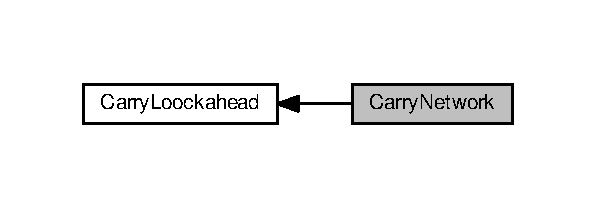
\includegraphics[width=286pt]{group___carry_network}
\end{center}
\end{figure}
\subsection*{Entities}
\begin{DoxyCompactItemize}
\item 
\hyperlink{classcla__carry__net}{cla\+\_\+carry\+\_\+net} entity
\begin{DoxyCompactList}\small\item\em Rete logica di calcolo dei riporti per un addizionatore a quattro bit con carry lookahead.

Permette di anticipare il calcolo dei riporti usando le funzioni \char`\"{}propagazione\char`\"{} e \char`\"{}generazione\char`\"{} prodotte dai singoli blocchi \hyperlink{classcla__adder__cell}{cla\+\_\+adder\+\_\+cell}, in modo da ridurre tempo necessario ad effettuare il calcolo di tutti i carry, quindi il tempo necessario a completare la somma. Questo blocco calcola solo i carry, pertanto va connesso ai blocchi \hyperlink{classcla__adder__cell}{cla\+\_\+adder\+\_\+cell}, per il calcolo materiale della somma, così come indicato dallo schema seguente, il quale rappresenta lo schema completo di un addizionatore a quattro bit\+: . \end{DoxyCompactList}\item 
\hyperlink{classcla__carry__net_1_1dataflow}{dataflow} architecture
\begin{DoxyCompactList}\small\item\em Implementazione dataflow dell\textquotesingle{}entita\textquotesingle{} \hyperlink{classcla__carry__net}{cla\+\_\+carry\+\_\+net}.

L\textquotesingle{}implementazione si basa sul seguente ragionamento\+: Proviamo ad esprimere, adesso, il carry carryout(i+1) in base alle funzioni gen(i) e prop(i), partendo, ad esempio, da carryout(1). Il carry carryout(0) varra\textquotesingle{} 1 se al passo precedente è stato generato riporto oppure se verra\textquotesingle{} propagato il carry carryin. In formule\+: \begin{center}carryout(0)=genin+(propin$\ast$carryin);\end{center}  Possiamo estendere lo stesso ragionamento a carryout(2)\+: \begin{center}carryout(1)=gen(1)+prop(1)$\ast$carryout(1)=gen(1)+prop(1)$\ast$gen(0)+prop(1)$\ast$prop(0)$\ast$carryin\end{center}  Cio\textquotesingle{} significa che il riporto carryout(1) lo si può esprimere sulla base di soli dati di ingresso con reti combinatorie a due livelli, senza utilizzare valori calcolati da nodi precedenti. Tutto ciò si traduce in un minor tempo necessario ad effettuare il calcolo di tutti i carry, quindi un minor tempo necessario a completare la somma. Purtroppo non si può procedere in questo modo ad oltranza per cui si tende a spezzare" la rete per il calcolo dei carry in blocchi più piccoli, ad esempio reti per il calcolo di carry per quattro bit. Considerando che \begin{center}carryout(4)=gen(3)+prop(3)$\ast$carryout(3)=...=genout+propout$\ast$carryin\end{center}  con \begin{center}genout=gen(3)+(prop(3)$\ast$gen(2))+(prop(3)$\ast$prop(2)$\ast$gen(1))+(prop(3)$\ast$prop(2)$\ast$prop(1)$\ast$gen(0))+(prop(3)$\ast$prop(2)$\ast$prop(1)$\ast$prop(0)$\ast$genin)\end{center}  \begin{center}propout=prop(3)$\ast$prop(2)$\ast$prop(1)$\ast$prop(0)$\ast$propin\end{center}  Si può costruire dei blocchi che presentino in uscita i segnali genout e propout, in modo da permettere ad eventuali blocchi successivi il calcolo veloce dei carry sulla base di questi segnali e del segnale carryin. \end{DoxyCompactList}\end{DoxyCompactItemize}
\subsection*{Ports}
 \begin{DoxyCompactItemize}
\item 
\hyperlink{group___carry_network_gac1f84cd3374a5a4d2ee2669ebdadafe8}{prop}  {\bfseries {\bfseries \textcolor{vhdlchar}{in}\textcolor{vhdlchar}{ }}} {\bfseries \textcolor{vhdlchar}{std\+\_\+logic\+\_\+vector}\textcolor{vhdlchar}{ }\textcolor{vhdlchar}{(}\textcolor{vhdlchar}{ }\textcolor{vhdlchar}{ } \textcolor{vhdldigit}{3} \textcolor{vhdlchar}{ }\textcolor{vhdlchar}{downto}\textcolor{vhdlchar}{ }\textcolor{vhdlchar}{ } \textcolor{vhdldigit}{0} \textcolor{vhdlchar}{ }\textcolor{vhdlchar}{)}\textcolor{vhdlchar}{ }} 
\item 
\hyperlink{group___carry_network_ga1ff97daaf4e03defc21748593cacfaa7}{gen}  {\bfseries {\bfseries \textcolor{vhdlchar}{in}\textcolor{vhdlchar}{ }}} {\bfseries \textcolor{vhdlchar}{std\+\_\+logic\+\_\+vector}\textcolor{vhdlchar}{ }\textcolor{vhdlchar}{(}\textcolor{vhdlchar}{ }\textcolor{vhdlchar}{ } \textcolor{vhdldigit}{3} \textcolor{vhdlchar}{ }\textcolor{vhdlchar}{downto}\textcolor{vhdlchar}{ }\textcolor{vhdlchar}{ } \textcolor{vhdldigit}{0} \textcolor{vhdlchar}{ }\textcolor{vhdlchar}{)}\textcolor{vhdlchar}{ }} 
\item 
\hyperlink{group___carry_network_gaa556a73dc4a4de1a0d662b25adbcbe33}{carryin}  {\bfseries {\bfseries \textcolor{vhdlchar}{in}\textcolor{vhdlchar}{ }}} {\bfseries \textcolor{vhdlchar}{std\+\_\+logic}\textcolor{vhdlchar}{ }} 
\begin{DoxyCompactList}\small\item\em segnale di \char`\"{}carry-\/in\char`\"{}, prodotto da un eventuale \hyperlink{classcla__carry__net}{cla\+\_\+carry\+\_\+net} a monte. \end{DoxyCompactList}\item 
\hyperlink{group___carry_network_ga422e8e7ee01fc7ac7b7390cd2ad8c87b}{propin}  {\bfseries {\bfseries \textcolor{vhdlchar}{in}\textcolor{vhdlchar}{ }}} {\bfseries \textcolor{vhdlchar}{std\+\_\+logic}\textcolor{vhdlchar}{ }} 
\begin{DoxyCompactList}\small\item\em funzione \char`\"{}propagazione\char`\"{}, prodotta da una eventuale \hyperlink{classcla__carry__net}{cla\+\_\+carry\+\_\+net} a monte \end{DoxyCompactList}\item 
\hyperlink{group___carry_network_ga0a46d5193cb73eb993bc5d4f69741d0a}{genin}  {\bfseries {\bfseries \textcolor{vhdlchar}{in}\textcolor{vhdlchar}{ }}} {\bfseries \textcolor{vhdlchar}{std\+\_\+logic}\textcolor{vhdlchar}{ }} 
\begin{DoxyCompactList}\small\item\em funzione \char`\"{}generazione\char`\"{}, prodotta da una eventuale \hyperlink{classcla__carry__net}{cla\+\_\+carry\+\_\+net} a monte \end{DoxyCompactList}\item 
\hyperlink{group___carry_network_ga6b265f3fe41195485dfedd9824c3598f}{carryout}  {\bfseries {\bfseries \textcolor{vhdlchar}{out}\textcolor{vhdlchar}{ }}} {\bfseries \textcolor{vhdlchar}{std\+\_\+logic\+\_\+vector}\textcolor{vhdlchar}{ }\textcolor{vhdlchar}{(}\textcolor{vhdlchar}{ }\textcolor{vhdlchar}{ } \textcolor{vhdldigit}{3} \textcolor{vhdlchar}{ }\textcolor{vhdlchar}{downto}\textcolor{vhdlchar}{ }\textcolor{vhdlchar}{ } \textcolor{vhdldigit}{0} \textcolor{vhdlchar}{ }\textcolor{vhdlchar}{)}\textcolor{vhdlchar}{ }} 
\item 
\hyperlink{group___carry_network_ga5957c9cdd706cafd2da8855133a002c9}{propout}  {\bfseries {\bfseries \textcolor{vhdlchar}{out}\textcolor{vhdlchar}{ }}} {\bfseries \textcolor{vhdlchar}{std\+\_\+logic}\textcolor{vhdlchar}{ }} 
\item 
\hyperlink{group___carry_network_ga068cd5c4d23e284cb942702252ed1491}{genout}  {\bfseries {\bfseries \textcolor{vhdlchar}{out}\textcolor{vhdlchar}{ }}} {\bfseries \textcolor{vhdlchar}{std\+\_\+logic}\textcolor{vhdlchar}{ }} 
\end{DoxyCompactItemize}


\subsection{Descrizione dettagliata}
Rete di generazione dei segnali di carry per un adder a quattro bit. 



\subsection{Documentazione delle variabili}
\index{Carry\+Network@{Carry\+Network}!carryin@{carryin}}
\index{carryin@{carryin}!Carry\+Network@{Carry\+Network}}
\subsubsection[{\texorpdfstring{carryin}{carryin}}]{\setlength{\rightskip}{0pt plus 5cm}{\bf carryin} {\bfseries \textcolor{vhdlchar}{in}\textcolor{vhdlchar}{ }} {\bfseries \textcolor{vhdlchar}{std\+\_\+logic}\textcolor{vhdlchar}{ }} \hspace{0.3cm}{\ttfamily [Port]}}\hypertarget{group___carry_network_gaa556a73dc4a4de1a0d662b25adbcbe33}{}\label{group___carry_network_gaa556a73dc4a4de1a0d662b25adbcbe33}


segnale di \char`\"{}carry-\/in\char`\"{}, prodotto da un eventuale \hyperlink{classcla__carry__net}{cla\+\_\+carry\+\_\+net} a monte. 

funzione \char`\"{}generazione\char`\"{} prodotta da \hyperlink{classcla__adder__cell}{cla\+\_\+adder\+\_\+cell}; vale 1 quando, sulla base degli ingressi, un adder generera\textquotesingle{} un carry in uscita; gen(i) = add(i) A\+ND add(i); in questo caso viene prodotta da quattro blocchi \hyperlink{classcla__adder__cell}{cla\+\_\+adder\+\_\+cell} sulla base dei loro ingressi \index{Carry\+Network@{Carry\+Network}!carryout@{carryout}}
\index{carryout@{carryout}!Carry\+Network@{Carry\+Network}}
\subsubsection[{\texorpdfstring{carryout}{carryout}}]{\setlength{\rightskip}{0pt plus 5cm}{\bf carryout} {\bfseries \textcolor{vhdlchar}{out}\textcolor{vhdlchar}{ }} {\bfseries \textcolor{vhdlchar}{std\+\_\+logic\+\_\+vector}\textcolor{vhdlchar}{ }\textcolor{vhdlchar}{(}\textcolor{vhdlchar}{ }\textcolor{vhdlchar}{ } \textcolor{vhdldigit}{3} \textcolor{vhdlchar}{ }\textcolor{vhdlchar}{downto}\textcolor{vhdlchar}{ }\textcolor{vhdlchar}{ } \textcolor{vhdldigit}{0} \textcolor{vhdlchar}{ }\textcolor{vhdlchar}{)}\textcolor{vhdlchar}{ }} \hspace{0.3cm}{\ttfamily [Port]}}\hypertarget{group___carry_network_ga6b265f3fe41195485dfedd9824c3598f}{}\label{group___carry_network_ga6b265f3fe41195485dfedd9824c3598f}
\index{Carry\+Network@{Carry\+Network}!gen@{gen}}
\index{gen@{gen}!Carry\+Network@{Carry\+Network}}
\subsubsection[{\texorpdfstring{gen}{gen}}]{\setlength{\rightskip}{0pt plus 5cm}{\bf gen} {\bfseries \textcolor{vhdlchar}{in}\textcolor{vhdlchar}{ }} {\bfseries \textcolor{vhdlchar}{std\+\_\+logic\+\_\+vector}\textcolor{vhdlchar}{ }\textcolor{vhdlchar}{(}\textcolor{vhdlchar}{ }\textcolor{vhdlchar}{ } \textcolor{vhdldigit}{3} \textcolor{vhdlchar}{ }\textcolor{vhdlchar}{downto}\textcolor{vhdlchar}{ }\textcolor{vhdlchar}{ } \textcolor{vhdldigit}{0} \textcolor{vhdlchar}{ }\textcolor{vhdlchar}{)}\textcolor{vhdlchar}{ }} \hspace{0.3cm}{\ttfamily [Port]}}\hypertarget{group___carry_network_ga1ff97daaf4e03defc21748593cacfaa7}{}\label{group___carry_network_ga1ff97daaf4e03defc21748593cacfaa7}
funzione “propagazione” prodotta da \hyperlink{classcla__adder__cell}{cla\+\_\+adder\+\_\+cell}; vale 1 quando, sulla base degli ingressi, un adder propaghera\textquotesingle{} un eventuale carry in ingresso; prop(i) = add(i) OR add(i); in questo caso viene prodotta da quattro blocchi \hyperlink{classcla__adder__cell}{cla\+\_\+adder\+\_\+cell} sulla base dei loro ingressi \index{Carry\+Network@{Carry\+Network}!genin@{genin}}
\index{genin@{genin}!Carry\+Network@{Carry\+Network}}
\subsubsection[{\texorpdfstring{genin}{genin}}]{\setlength{\rightskip}{0pt plus 5cm}{\bf genin} {\bfseries \textcolor{vhdlchar}{in}\textcolor{vhdlchar}{ }} {\bfseries \textcolor{vhdlchar}{std\+\_\+logic}\textcolor{vhdlchar}{ }} \hspace{0.3cm}{\ttfamily [Port]}}\hypertarget{group___carry_network_ga0a46d5193cb73eb993bc5d4f69741d0a}{}\label{group___carry_network_ga0a46d5193cb73eb993bc5d4f69741d0a}


funzione \char`\"{}generazione\char`\"{}, prodotta da una eventuale \hyperlink{classcla__carry__net}{cla\+\_\+carry\+\_\+net} a monte 

\index{Carry\+Network@{Carry\+Network}!genout@{genout}}
\index{genout@{genout}!Carry\+Network@{Carry\+Network}}
\subsubsection[{\texorpdfstring{genout}{genout}}]{\setlength{\rightskip}{0pt plus 5cm}{\bf genout} {\bfseries \textcolor{vhdlchar}{out}\textcolor{vhdlchar}{ }} {\bfseries \textcolor{vhdlchar}{std\+\_\+logic}\textcolor{vhdlchar}{ }} \hspace{0.3cm}{\ttfamily [Port]}}\hypertarget{group___carry_network_ga068cd5c4d23e284cb942702252ed1491}{}\label{group___carry_network_ga068cd5c4d23e284cb942702252ed1491}
funzione \char`\"{}propagazione\char`\"{} da porre in ingresso ad un eventuale blocco \hyperlink{classcla__carry__net}{cla\+\_\+carry\+\_\+net} a valle \index{Carry\+Network@{Carry\+Network}!prop@{prop}}
\index{prop@{prop}!Carry\+Network@{Carry\+Network}}
\subsubsection[{\texorpdfstring{prop}{prop}}]{\setlength{\rightskip}{0pt plus 5cm}{\bf prop} {\bfseries \textcolor{vhdlchar}{in}\textcolor{vhdlchar}{ }} {\bfseries \textcolor{vhdlchar}{std\+\_\+logic\+\_\+vector}\textcolor{vhdlchar}{ }\textcolor{vhdlchar}{(}\textcolor{vhdlchar}{ }\textcolor{vhdlchar}{ } \textcolor{vhdldigit}{3} \textcolor{vhdlchar}{ }\textcolor{vhdlchar}{downto}\textcolor{vhdlchar}{ }\textcolor{vhdlchar}{ } \textcolor{vhdldigit}{0} \textcolor{vhdlchar}{ }\textcolor{vhdlchar}{)}\textcolor{vhdlchar}{ }} \hspace{0.3cm}{\ttfamily [Port]}}\hypertarget{group___carry_network_gac1f84cd3374a5a4d2ee2669ebdadafe8}{}\label{group___carry_network_gac1f84cd3374a5a4d2ee2669ebdadafe8}
\index{Carry\+Network@{Carry\+Network}!propin@{propin}}
\index{propin@{propin}!Carry\+Network@{Carry\+Network}}
\subsubsection[{\texorpdfstring{propin}{propin}}]{\setlength{\rightskip}{0pt plus 5cm}{\bf propin} {\bfseries \textcolor{vhdlchar}{in}\textcolor{vhdlchar}{ }} {\bfseries \textcolor{vhdlchar}{std\+\_\+logic}\textcolor{vhdlchar}{ }} \hspace{0.3cm}{\ttfamily [Port]}}\hypertarget{group___carry_network_ga422e8e7ee01fc7ac7b7390cd2ad8c87b}{}\label{group___carry_network_ga422e8e7ee01fc7ac7b7390cd2ad8c87b}


funzione \char`\"{}propagazione\char`\"{}, prodotta da una eventuale \hyperlink{classcla__carry__net}{cla\+\_\+carry\+\_\+net} a monte 

\index{Carry\+Network@{Carry\+Network}!propout@{propout}}
\index{propout@{propout}!Carry\+Network@{Carry\+Network}}
\subsubsection[{\texorpdfstring{propout}{propout}}]{\setlength{\rightskip}{0pt plus 5cm}{\bf propout} {\bfseries \textcolor{vhdlchar}{out}\textcolor{vhdlchar}{ }} {\bfseries \textcolor{vhdlchar}{std\+\_\+logic}\textcolor{vhdlchar}{ }} \hspace{0.3cm}{\ttfamily [Port]}}\hypertarget{group___carry_network_ga5957c9cdd706cafd2da8855133a002c9}{}\label{group___carry_network_ga5957c9cdd706cafd2da8855133a002c9}
carry calcolati sulla base delle funzioni \char`\"{}propagazione\char`\"{} e \char`\"{}generazione\char`\"{} prodotti dai blocchi \hyperlink{classcla__adder__cell}{cla\+\_\+adder\+\_\+cell}, e sulla base delle funzioni \char`\"{}carry-\/in\char`\"{}, \char`\"{}propagazione\char`\"{} e \char`\"{}generazione\char`\"{} prodotti da eventuali blocchi a monte; ciascuno dei bit dovra\textquotesingle{} essere posto in ingresso ad un blocco \hyperlink{classcla__adder__cell}{cla\+\_\+adder\+\_\+cell} differente, affinche\textquotesingle{} possa essere calcolata la somma degli addendi 
\hypertarget{group___nibble_adder}{}\section{Nibble\+Adder}
\label{group___nibble_adder}\index{Nibble\+Adder@{Nibble\+Adder}}


Blocco elementare di somma a quattro bit.  


Diagramma di collaborazione per Nibble\+Adder\+:\nopagebreak
\begin{figure}[H]
\begin{center}
\leavevmode
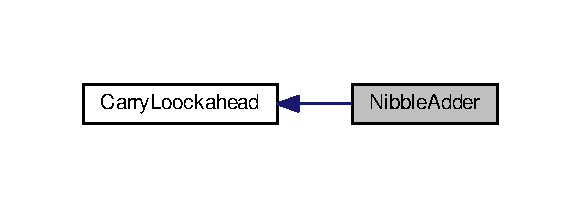
\includegraphics[width=279pt]{group___nibble_adder}
\end{center}
\end{figure}
\subsection*{Entities}
\begin{DoxyCompactItemize}
\item 
\hyperlink{classnibble__adder}{nibble\+\_\+adder} entity
\begin{DoxyCompactList}\small\item\em Addizionatore con carry-\/lookahead a quattro bit.

La cella somma tra loro due addendi ed un carry in ingresso; gli addendi sono espressi su quattro bit. Oltre a generare la somma, genera le funzioni \char`\"{}propagazione\char`\"{} e \char`\"{}generazione\char`\"{} del carry per eventuali blocchi \hyperlink{classnibble__adder}{nibble\+\_\+adder} posti a valle. \end{DoxyCompactList}\item 
\hyperlink{classnibble__adder_1_1structural}{structural} architecture
\begin{DoxyCompactList}\small\item\em Implementazione structural dell\textquotesingle{}entità \hyperlink{classnibble__adder}{nibble\+\_\+adder}.

Questa architettura istanzia una entità \hyperlink{classcla__carry__net}{cla\+\_\+carry\+\_\+net} ed una entità \hyperlink{classcla__adder__cell}{cla\+\_\+adder\+\_\+cell} per ogni bit su cui sono espressi gli addendi, connettendoli tra loro secondo lo schema riportato di seguito\+: . \end{DoxyCompactList}\end{DoxyCompactItemize}
\subsection*{Components}
 \begin{DoxyCompactItemize}
\item 
\hyperlink{group___nibble_adder_ga12bdc5892f526938e1447d663d152df8}{cla\+\_\+carry\+\_\+net}  {\bfseries }  
\item 
\hyperlink{group___nibble_adder_ga4f13eb52457f650b1d2cd352d9cacca9}{cla\+\_\+adder\+\_\+cell}  {\bfseries }  
\end{DoxyCompactItemize}
\subsection*{Ports}
 \begin{DoxyCompactItemize}
\item 
\hyperlink{group___nibble_adder_ga2c8945f4747b9a5448412c95fc281c87}{addendum1}  {\bfseries {\bfseries \textcolor{vhdlchar}{in}\textcolor{vhdlchar}{ }}} {\bfseries \textcolor{vhdlchar}{std\+\_\+logic\+\_\+vector}\textcolor{vhdlchar}{ }\textcolor{vhdlchar}{(}\textcolor{vhdlchar}{ }\textcolor{vhdlchar}{ } \textcolor{vhdldigit}{3} \textcolor{vhdlchar}{ }\textcolor{vhdlchar}{downto}\textcolor{vhdlchar}{ }\textcolor{vhdlchar}{ } \textcolor{vhdldigit}{0} \textcolor{vhdlchar}{ }\textcolor{vhdlchar}{)}\textcolor{vhdlchar}{ }} 
\begin{DoxyCompactList}\small\item\em addendo 1 \end{DoxyCompactList}\item 
\hyperlink{group___nibble_adder_gad1fa6d9d78208885ad2f4c417fc4b530}{addendum2}  {\bfseries {\bfseries \textcolor{vhdlchar}{in}\textcolor{vhdlchar}{ }}} {\bfseries \textcolor{vhdlchar}{std\+\_\+logic\+\_\+vector}\textcolor{vhdlchar}{ }\textcolor{vhdlchar}{(}\textcolor{vhdlchar}{ }\textcolor{vhdlchar}{ } \textcolor{vhdldigit}{3} \textcolor{vhdlchar}{ }\textcolor{vhdlchar}{downto}\textcolor{vhdlchar}{ }\textcolor{vhdlchar}{ } \textcolor{vhdldigit}{0} \textcolor{vhdlchar}{ }\textcolor{vhdlchar}{)}\textcolor{vhdlchar}{ }} 
\begin{DoxyCompactList}\small\item\em addendo 2 \end{DoxyCompactList}\item 
\hyperlink{group___nibble_adder_gaa556a73dc4a4de1a0d662b25adbcbe33}{carryin}  {\bfseries {\bfseries \textcolor{vhdlchar}{in}\textcolor{vhdlchar}{ }}} {\bfseries \textcolor{vhdlchar}{std\+\_\+logic}\textcolor{vhdlchar}{ }} 
\begin{DoxyCompactList}\small\item\em segnale di \char`\"{}carry-\/in\char`\"{}, prodotto da un eventuale \hyperlink{classnibble__adder}{nibble\+\_\+adder} a monte. \end{DoxyCompactList}\item 
\hyperlink{group___nibble_adder_ga422e8e7ee01fc7ac7b7390cd2ad8c87b}{propin}  {\bfseries {\bfseries \textcolor{vhdlchar}{in}\textcolor{vhdlchar}{ }}} {\bfseries \textcolor{vhdlchar}{std\+\_\+logic}\textcolor{vhdlchar}{ }} 
\begin{DoxyCompactList}\small\item\em funzione \char`\"{}propagazione\char`\"{}, prodotta da una eventuale \hyperlink{classnibble__adder}{nibble\+\_\+adder} a monte \end{DoxyCompactList}\item 
\hyperlink{group___nibble_adder_ga0a46d5193cb73eb993bc5d4f69741d0a}{genin}  {\bfseries {\bfseries \textcolor{vhdlchar}{in}\textcolor{vhdlchar}{ }}} {\bfseries \textcolor{vhdlchar}{std\+\_\+logic}\textcolor{vhdlchar}{ }} 
\begin{DoxyCompactList}\small\item\em funzione \char`\"{}generazione\char`\"{}, prodotta da una eventuale \hyperlink{classnibble__adder}{nibble\+\_\+adder} a monte \end{DoxyCompactList}\item 
\hyperlink{group___nibble_adder_ga5957c9cdd706cafd2da8855133a002c9}{propout}  {\bfseries {\bfseries \textcolor{vhdlchar}{out}\textcolor{vhdlchar}{ }}} {\bfseries \textcolor{vhdlchar}{std\+\_\+logic}\textcolor{vhdlchar}{ }} 
\item 
\hyperlink{group___nibble_adder_ga068cd5c4d23e284cb942702252ed1491}{genout}  {\bfseries {\bfseries \textcolor{vhdlchar}{out}\textcolor{vhdlchar}{ }}} {\bfseries \textcolor{vhdlchar}{std\+\_\+logic}\textcolor{vhdlchar}{ }} 
\item 
\hyperlink{group___nibble_adder_gadfe538323c3296159dd3b383325a996b}{sum}  {\bfseries {\bfseries \textcolor{vhdlchar}{out}\textcolor{vhdlchar}{ }}} {\bfseries \textcolor{vhdlchar}{std\+\_\+logic\+\_\+vector}\textcolor{vhdlchar}{ }\textcolor{vhdlchar}{(}\textcolor{vhdlchar}{ }\textcolor{vhdlchar}{ } \textcolor{vhdldigit}{3} \textcolor{vhdlchar}{ }\textcolor{vhdlchar}{downto}\textcolor{vhdlchar}{ }\textcolor{vhdlchar}{ } \textcolor{vhdldigit}{0} \textcolor{vhdlchar}{ }\textcolor{vhdlchar}{)}\textcolor{vhdlchar}{ }} 
\end{DoxyCompactItemize}
\subsection*{Signals}
 \begin{DoxyCompactItemize}
\item 
\hyperlink{group___nibble_adder_ga3abd8d433ff039baabc0c6fc2126578b}{prop} {\bfseries \textcolor{vhdlchar}{std\+\_\+logic\+\_\+vector}\textcolor{vhdlchar}{ }\textcolor{vhdlchar}{(}\textcolor{vhdlchar}{ }\textcolor{vhdlchar}{ } \textcolor{vhdldigit}{3} \textcolor{vhdlchar}{ }\textcolor{vhdlchar}{downto}\textcolor{vhdlchar}{ }\textcolor{vhdlchar}{ } \textcolor{vhdldigit}{0} \textcolor{vhdlchar}{ }\textcolor{vhdlchar}{)}\textcolor{vhdlchar}{ }} 
\item 
\hyperlink{group___nibble_adder_gac6c069fe4ec1c0a42272d3de4be6f45f}{gen} {\bfseries \textcolor{vhdlchar}{std\+\_\+logic\+\_\+vector}\textcolor{vhdlchar}{ }\textcolor{vhdlchar}{(}\textcolor{vhdlchar}{ }\textcolor{vhdlchar}{ } \textcolor{vhdldigit}{3} \textcolor{vhdlchar}{ }\textcolor{vhdlchar}{downto}\textcolor{vhdlchar}{ }\textcolor{vhdlchar}{ } \textcolor{vhdldigit}{0} \textcolor{vhdlchar}{ }\textcolor{vhdlchar}{)}\textcolor{vhdlchar}{ }} 
\item 
\hyperlink{group___nibble_adder_ga8f5524d80e551d479327a16bb32abcaa}{carry} {\bfseries \textcolor{vhdlchar}{std\+\_\+logic\+\_\+vector}\textcolor{vhdlchar}{ }\textcolor{vhdlchar}{(}\textcolor{vhdlchar}{ }\textcolor{vhdlchar}{ } \textcolor{vhdldigit}{3} \textcolor{vhdlchar}{ }\textcolor{vhdlchar}{downto}\textcolor{vhdlchar}{ }\textcolor{vhdlchar}{ } \textcolor{vhdldigit}{0} \textcolor{vhdlchar}{ }\textcolor{vhdlchar}{)}\textcolor{vhdlchar}{ }} 
\end{DoxyCompactItemize}


\subsection{Descrizione dettagliata}
Blocco elementare di somma a quattro bit. 



\subsection{Documentazione delle variabili}
\mbox{\Hypertarget{group___nibble_adder_ga2c8945f4747b9a5448412c95fc281c87}\label{group___nibble_adder_ga2c8945f4747b9a5448412c95fc281c87}} 
\index{Nibble\+Adder@{Nibble\+Adder}!addendum1@{addendum1}}
\index{addendum1@{addendum1}!Nibble\+Adder@{Nibble\+Adder}}
\subsubsection{\texorpdfstring{addendum1}{addendum1}}
{\footnotesize\ttfamily \hyperlink{group___nibble_adder_ga2c8945f4747b9a5448412c95fc281c87}{addendum1} {\bfseries \textcolor{vhdlchar}{in}\textcolor{vhdlchar}{ }} {\bfseries \textcolor{vhdlchar}{std\+\_\+logic\+\_\+vector}\textcolor{vhdlchar}{ }\textcolor{vhdlchar}{(}\textcolor{vhdlchar}{ }\textcolor{vhdlchar}{ } \textcolor{vhdldigit}{3} \textcolor{vhdlchar}{ }\textcolor{vhdlchar}{downto}\textcolor{vhdlchar}{ }\textcolor{vhdlchar}{ } \textcolor{vhdldigit}{0} \textcolor{vhdlchar}{ }\textcolor{vhdlchar}{)}\textcolor{vhdlchar}{ }} \hspace{0.3cm}{\ttfamily [Port]}}



addendo 1 

\mbox{\Hypertarget{group___nibble_adder_gad1fa6d9d78208885ad2f4c417fc4b530}\label{group___nibble_adder_gad1fa6d9d78208885ad2f4c417fc4b530}} 
\index{Nibble\+Adder@{Nibble\+Adder}!addendum2@{addendum2}}
\index{addendum2@{addendum2}!Nibble\+Adder@{Nibble\+Adder}}
\subsubsection{\texorpdfstring{addendum2}{addendum2}}
{\footnotesize\ttfamily \hyperlink{group___nibble_adder_gad1fa6d9d78208885ad2f4c417fc4b530}{addendum2} {\bfseries \textcolor{vhdlchar}{in}\textcolor{vhdlchar}{ }} {\bfseries \textcolor{vhdlchar}{std\+\_\+logic\+\_\+vector}\textcolor{vhdlchar}{ }\textcolor{vhdlchar}{(}\textcolor{vhdlchar}{ }\textcolor{vhdlchar}{ } \textcolor{vhdldigit}{3} \textcolor{vhdlchar}{ }\textcolor{vhdlchar}{downto}\textcolor{vhdlchar}{ }\textcolor{vhdlchar}{ } \textcolor{vhdldigit}{0} \textcolor{vhdlchar}{ }\textcolor{vhdlchar}{)}\textcolor{vhdlchar}{ }} \hspace{0.3cm}{\ttfamily [Port]}}



addendo 2 

\mbox{\Hypertarget{group___nibble_adder_ga8f5524d80e551d479327a16bb32abcaa}\label{group___nibble_adder_ga8f5524d80e551d479327a16bb32abcaa}} 
\index{Nibble\+Adder@{Nibble\+Adder}!carry@{carry}}
\index{carry@{carry}!Nibble\+Adder@{Nibble\+Adder}}
\subsubsection{\texorpdfstring{carry}{carry}}
{\footnotesize\ttfamily \hyperlink{group___nibble_adder_ga8f5524d80e551d479327a16bb32abcaa}{carry} {\bfseries \textcolor{vhdlchar}{std\+\_\+logic\+\_\+vector}\textcolor{vhdlchar}{ }\textcolor{vhdlchar}{(}\textcolor{vhdlchar}{ }\textcolor{vhdlchar}{ } \textcolor{vhdldigit}{3} \textcolor{vhdlchar}{ }\textcolor{vhdlchar}{downto}\textcolor{vhdlchar}{ }\textcolor{vhdlchar}{ } \textcolor{vhdldigit}{0} \textcolor{vhdlchar}{ }\textcolor{vhdlchar}{)}\textcolor{vhdlchar}{ }} \hspace{0.3cm}{\ttfamily [Signal]}}

funzione \char`\"{}generazione\char`\"{} prodotta da \hyperlink{classcla__adder__cell}{cla\+\_\+adder\+\_\+cell}; vale 1 quando, sulla base degli ingressi, un adder generera\textquotesingle{} un carry in uscita; gen(i) = add(i) A\+ND add(i); in questo caso viene prodotta da quattro blocchi \hyperlink{classcla__adder__cell}{cla\+\_\+adder\+\_\+cell} sulla base dei loro ingressi \mbox{\Hypertarget{group___nibble_adder_gaa556a73dc4a4de1a0d662b25adbcbe33}\label{group___nibble_adder_gaa556a73dc4a4de1a0d662b25adbcbe33}} 
\index{Nibble\+Adder@{Nibble\+Adder}!carryin@{carryin}}
\index{carryin@{carryin}!Nibble\+Adder@{Nibble\+Adder}}
\subsubsection{\texorpdfstring{carryin}{carryin}}
{\footnotesize\ttfamily \hyperlink{group___nibble_adder_gaa556a73dc4a4de1a0d662b25adbcbe33}{carryin} {\bfseries \textcolor{vhdlchar}{in}\textcolor{vhdlchar}{ }} {\bfseries \textcolor{vhdlchar}{std\+\_\+logic}\textcolor{vhdlchar}{ }} \hspace{0.3cm}{\ttfamily [Port]}}



segnale di \char`\"{}carry-\/in\char`\"{}, prodotto da un eventuale \hyperlink{classnibble__adder}{nibble\+\_\+adder} a monte. 

\mbox{\Hypertarget{group___nibble_adder_ga4f13eb52457f650b1d2cd352d9cacca9}\label{group___nibble_adder_ga4f13eb52457f650b1d2cd352d9cacca9}} 
\index{Nibble\+Adder@{Nibble\+Adder}!cla\+\_\+adder\+\_\+cell@{cla\+\_\+adder\+\_\+cell}}
\index{cla\+\_\+adder\+\_\+cell@{cla\+\_\+adder\+\_\+cell}!Nibble\+Adder@{Nibble\+Adder}}
\subsubsection{\texorpdfstring{cla\+\_\+adder\+\_\+cell}{cla\_adder\_cell}}
{\footnotesize\ttfamily \hyperlink{group___nibble_adder_ga4f13eb52457f650b1d2cd352d9cacca9}{cla\+\_\+adder\+\_\+cell} {\bfseries \textcolor{vhdlchar}{ }} \hspace{0.3cm}{\ttfamily [Component]}}

\mbox{\Hypertarget{group___nibble_adder_ga12bdc5892f526938e1447d663d152df8}\label{group___nibble_adder_ga12bdc5892f526938e1447d663d152df8}} 
\index{Nibble\+Adder@{Nibble\+Adder}!cla\+\_\+carry\+\_\+net@{cla\+\_\+carry\+\_\+net}}
\index{cla\+\_\+carry\+\_\+net@{cla\+\_\+carry\+\_\+net}!Nibble\+Adder@{Nibble\+Adder}}
\subsubsection{\texorpdfstring{cla\+\_\+carry\+\_\+net}{cla\_carry\_net}}
{\footnotesize\ttfamily \hyperlink{group___nibble_adder_ga12bdc5892f526938e1447d663d152df8}{cla\+\_\+carry\+\_\+net} {\bfseries \textcolor{vhdlchar}{ }} \hspace{0.3cm}{\ttfamily [Component]}}

\mbox{\Hypertarget{group___nibble_adder_gac6c069fe4ec1c0a42272d3de4be6f45f}\label{group___nibble_adder_gac6c069fe4ec1c0a42272d3de4be6f45f}} 
\index{Nibble\+Adder@{Nibble\+Adder}!gen@{gen}}
\index{gen@{gen}!Nibble\+Adder@{Nibble\+Adder}}
\subsubsection{\texorpdfstring{gen}{gen}}
{\footnotesize\ttfamily \hyperlink{group___nibble_adder_gac6c069fe4ec1c0a42272d3de4be6f45f}{gen} {\bfseries \textcolor{vhdlchar}{std\+\_\+logic\+\_\+vector}\textcolor{vhdlchar}{ }\textcolor{vhdlchar}{(}\textcolor{vhdlchar}{ }\textcolor{vhdlchar}{ } \textcolor{vhdldigit}{3} \textcolor{vhdlchar}{ }\textcolor{vhdlchar}{downto}\textcolor{vhdlchar}{ }\textcolor{vhdlchar}{ } \textcolor{vhdldigit}{0} \textcolor{vhdlchar}{ }\textcolor{vhdlchar}{)}\textcolor{vhdlchar}{ }} \hspace{0.3cm}{\ttfamily [Signal]}}

funzione “propagazione” prodotta da \hyperlink{classcla__adder__cell}{cla\+\_\+adder\+\_\+cell}; vale 1 quando, sulla base degli ingressi, un adder propaghera\textquotesingle{} un eventuale carry in ingresso; prop(i) = add(i) OR add(i); in questo caso viene prodotta da quattro blocchi \hyperlink{classcla__adder__cell}{cla\+\_\+adder\+\_\+cell} sulla base dei loro ingressi \mbox{\Hypertarget{group___nibble_adder_ga0a46d5193cb73eb993bc5d4f69741d0a}\label{group___nibble_adder_ga0a46d5193cb73eb993bc5d4f69741d0a}} 
\index{Nibble\+Adder@{Nibble\+Adder}!genin@{genin}}
\index{genin@{genin}!Nibble\+Adder@{Nibble\+Adder}}
\subsubsection{\texorpdfstring{genin}{genin}}
{\footnotesize\ttfamily \hyperlink{group___nibble_adder_ga0a46d5193cb73eb993bc5d4f69741d0a}{genin} {\bfseries \textcolor{vhdlchar}{in}\textcolor{vhdlchar}{ }} {\bfseries \textcolor{vhdlchar}{std\+\_\+logic}\textcolor{vhdlchar}{ }} \hspace{0.3cm}{\ttfamily [Port]}}



funzione \char`\"{}generazione\char`\"{}, prodotta da una eventuale \hyperlink{classnibble__adder}{nibble\+\_\+adder} a monte 

\mbox{\Hypertarget{group___nibble_adder_ga068cd5c4d23e284cb942702252ed1491}\label{group___nibble_adder_ga068cd5c4d23e284cb942702252ed1491}} 
\index{Nibble\+Adder@{Nibble\+Adder}!genout@{genout}}
\index{genout@{genout}!Nibble\+Adder@{Nibble\+Adder}}
\subsubsection{\texorpdfstring{genout}{genout}}
{\footnotesize\ttfamily \hyperlink{group___nibble_adder_ga068cd5c4d23e284cb942702252ed1491}{genout} {\bfseries \textcolor{vhdlchar}{out}\textcolor{vhdlchar}{ }} {\bfseries \textcolor{vhdlchar}{std\+\_\+logic}\textcolor{vhdlchar}{ }} \hspace{0.3cm}{\ttfamily [Port]}}

funzione \char`\"{}propagazione\char`\"{} da porre in ingresso ad un eventuale blocco \hyperlink{classnibble__adder}{nibble\+\_\+adder} a valle \mbox{\Hypertarget{group___nibble_adder_ga3abd8d433ff039baabc0c6fc2126578b}\label{group___nibble_adder_ga3abd8d433ff039baabc0c6fc2126578b}} 
\index{Nibble\+Adder@{Nibble\+Adder}!prop@{prop}}
\index{prop@{prop}!Nibble\+Adder@{Nibble\+Adder}}
\subsubsection{\texorpdfstring{prop}{prop}}
{\footnotesize\ttfamily \hyperlink{group___nibble_adder_ga3abd8d433ff039baabc0c6fc2126578b}{prop} {\bfseries \textcolor{vhdlchar}{std\+\_\+logic\+\_\+vector}\textcolor{vhdlchar}{ }\textcolor{vhdlchar}{(}\textcolor{vhdlchar}{ }\textcolor{vhdlchar}{ } \textcolor{vhdldigit}{3} \textcolor{vhdlchar}{ }\textcolor{vhdlchar}{downto}\textcolor{vhdlchar}{ }\textcolor{vhdlchar}{ } \textcolor{vhdldigit}{0} \textcolor{vhdlchar}{ }\textcolor{vhdlchar}{)}\textcolor{vhdlchar}{ }} \hspace{0.3cm}{\ttfamily [Signal]}}

\mbox{\Hypertarget{group___nibble_adder_ga422e8e7ee01fc7ac7b7390cd2ad8c87b}\label{group___nibble_adder_ga422e8e7ee01fc7ac7b7390cd2ad8c87b}} 
\index{Nibble\+Adder@{Nibble\+Adder}!propin@{propin}}
\index{propin@{propin}!Nibble\+Adder@{Nibble\+Adder}}
\subsubsection{\texorpdfstring{propin}{propin}}
{\footnotesize\ttfamily \hyperlink{group___nibble_adder_ga422e8e7ee01fc7ac7b7390cd2ad8c87b}{propin} {\bfseries \textcolor{vhdlchar}{in}\textcolor{vhdlchar}{ }} {\bfseries \textcolor{vhdlchar}{std\+\_\+logic}\textcolor{vhdlchar}{ }} \hspace{0.3cm}{\ttfamily [Port]}}



funzione \char`\"{}propagazione\char`\"{}, prodotta da una eventuale \hyperlink{classnibble__adder}{nibble\+\_\+adder} a monte 

\mbox{\Hypertarget{group___nibble_adder_ga5957c9cdd706cafd2da8855133a002c9}\label{group___nibble_adder_ga5957c9cdd706cafd2da8855133a002c9}} 
\index{Nibble\+Adder@{Nibble\+Adder}!propout@{propout}}
\index{propout@{propout}!Nibble\+Adder@{Nibble\+Adder}}
\subsubsection{\texorpdfstring{propout}{propout}}
{\footnotesize\ttfamily \hyperlink{group___nibble_adder_ga5957c9cdd706cafd2da8855133a002c9}{propout} {\bfseries \textcolor{vhdlchar}{out}\textcolor{vhdlchar}{ }} {\bfseries \textcolor{vhdlchar}{std\+\_\+logic}\textcolor{vhdlchar}{ }} \hspace{0.3cm}{\ttfamily [Port]}}

\mbox{\Hypertarget{group___nibble_adder_gadfe538323c3296159dd3b383325a996b}\label{group___nibble_adder_gadfe538323c3296159dd3b383325a996b}} 
\index{Nibble\+Adder@{Nibble\+Adder}!sum@{sum}}
\index{sum@{sum}!Nibble\+Adder@{Nibble\+Adder}}
\subsubsection{\texorpdfstring{sum}{sum}}
{\footnotesize\ttfamily \hyperlink{group___nibble_adder_gadfe538323c3296159dd3b383325a996b}{sum} {\bfseries \textcolor{vhdlchar}{out}\textcolor{vhdlchar}{ }} {\bfseries \textcolor{vhdlchar}{std\+\_\+logic\+\_\+vector}\textcolor{vhdlchar}{ }\textcolor{vhdlchar}{(}\textcolor{vhdlchar}{ }\textcolor{vhdlchar}{ } \textcolor{vhdldigit}{3} \textcolor{vhdlchar}{ }\textcolor{vhdlchar}{downto}\textcolor{vhdlchar}{ }\textcolor{vhdlchar}{ } \textcolor{vhdldigit}{0} \textcolor{vhdlchar}{ }\textcolor{vhdlchar}{)}\textcolor{vhdlchar}{ }} \hspace{0.3cm}{\ttfamily [Port]}}

funzione \char`\"{}generazione\char`\"{} da porre in ingresso ad un eventuale blocco \hyperlink{classnibble__adder}{nibble\+\_\+adder} a valle 
\hypertarget{group___linear_regression}{}\section{Linear\+Regression}
\label{group___linear_regression}\index{Linear\+Regression@{Linear\+Regression}}


Regressione Lineare in V\+H\+DL.  


\subsection*{Entities}
\begin{DoxyCompactItemize}
\item 
\hyperlink{class_linear_regression}{Linear\+Regression} entity
\item 
\hyperlink{class_linear_regression_1_1_structural}{Structural} architecture
\begin{DoxyCompactList}\small\item\em 8 

M\+U\+L\+T1, M\+U\+L\+T2, M\+U\+L\+T3, M\+U\+L\+T4, A\+D\+D5, A\+D\+D6, M\+U\+L\+T6 

Verificare che il troncamento post M\+U\+L\+T6 venga effettuato correttamente (7 bit in testa e 17 in coda) 

C=b\char`\"{}011000011101000101011010\char`\"{}~\newline
 Sum2=b\char`\"{}001010111100110111101111\char`\"{}~\newline
 B=b\char`\"{}001000110100010101100111\char`\"{}~\newline
 Sum1=b\char`\"{}001101001011110110010011\char`\"{}~\newline
 A=b\char`\"{}000111101111000111001010\char`\"{}  

mult2\+\_\+out=b\char`\"{}000001100000100100000111110011100100011000101001\char`\"{}~\newline
 P2= b\char`\"{}000010010000011111001110\char`\"{}~\newline
 mult4\+\_\+out=b\char`\"{}000101000010011011110110000000101010100010101110\char`\"{}~\newline
 P4= b\char`\"{}001010000100110111101100\char`\"{}~\newline
 add2\+\_\+out= b\char`\"{}001100010101010110111010\char`\"{}~\newline
 S6= b\char`\"{}000110001010101011011101\char`\"{}~\newline
 mult1\+\_\+out=b\char`\"{}00001101101100000101101010110\char`\"{}~\newline
 P3= b\char`\"{}011011011000001011010101\char`\"{}~\newline
 mult3\+\_\+out=b\char`\"{}000001110100010000110111011010011110010100100101\char`\"{}~\newline
 P1= b\char`\"{}110100010000110111011010\char`\"{}~\newline
 S5= b\char`\"{}001111101001000010101111\char`\"{}~\newline
 mult6\+\_\+out=b\char`\"{}000000101111101101010010001101101101111101100010\char`\"{}~\newline
 q =b\char`\"{}011111011010100100011011\char`\"{}  

mult2\+\_\+out=b\char`\"{}000001100000100100000111110011100100011000101001\char`\"{}~\newline
 P2= b\char`\"{}000010010000011111001110\char`\"{}~\newline
 mult4\+\_\+out=b\char`\"{}000101000010011011110110000000101010100010101110\char`\"{}~\newline
 P4= b\char`\"{}001010000100110111101100\char`\"{}~\newline
 add2\+\_\+out= b\char`\"{}001100010101010110111010\char`\"{}~\newline
 S6= b\char`\"{}000110001010101011011101\char`\"{}~\newline
 mult1\+\_\+out=b\char`\"{}00001101101100000101101010110\char`\"{}~\newline
 P3= b\char`\"{}011011011000001011010101\char`\"{}~\newline
 mult3\+\_\+out=b\char`\"{}000001110100010000110111011010011110010100100101\char`\"{}~\newline
 P1= b\char`\"{}110100010000110111011010\char`\"{}~\newline
 S5= b\char`\"{}001111101001000010101111\char`\"{}~\newline
 mult6\+\_\+out=b\char`\"{}000000101111101101010010001101101101111101100010\char`\"{}~\newline
 q =b\char`\"{}       011111011010100100011011\char`\"{}  

Superato  \end{DoxyCompactList}\end{DoxyCompactItemize}
\subsection*{Libraries}
 \begin{DoxyCompactItemize}
\item 
\hyperlink{group___linear_regression_gae4f03c286607f3181e16b9aa12d0c6d4}{I\+E\+EE} 
\end{DoxyCompactItemize}
\subsection*{Use Clauses}
 \begin{DoxyCompactItemize}
\item 
\hyperlink{group___linear_regression_gaa4b2b25246a821511120e3149b003563}{S\+T\+D\+\_\+\+L\+O\+G\+I\+C\+\_\+1164}   
\item 
\hyperlink{group___linear_regression_gae00f3f04545af57582ff10609eee23e2}{N\+U\+M\+E\+R\+I\+C\+\_\+\+S\+TD}   
\end{DoxyCompactItemize}
\subsection*{Components}
 \begin{DoxyCompactItemize}
\item 
\hyperlink{group___linear_regression_ga3cf9cbfc3e637ae0660c32ceef50386f}{multiplier}  {\bfseries }  
\item 
\hyperlink{group___linear_regression_ga9d7a8a381439c61aea549e7a47ec7a6f}{adder}  {\bfseries }  
\end{DoxyCompactItemize}
\subsection*{Ports}
 \begin{DoxyCompactItemize}
\item 
\hyperlink{group___linear_regression_ga6b9afe9c48db695b7336519281c099a8}{prim}  {\bfseries {\bfseries \textcolor{vhdlchar}{in}\textcolor{vhdlchar}{ }}} {\bfseries \textcolor{vhdlchar}{S\+T\+D\+\_\+\+L\+O\+G\+I\+C\+\_\+\+V\+E\+C\+T\+OR}\textcolor{vhdlchar}{ }\textcolor{vhdlchar}{(}\textcolor{vhdlchar}{ }\textcolor{vhdlchar}{ } \textcolor{vhdldigit}{4} \textcolor{vhdlchar}{ }\textcolor{vhdlchar}{downto}\textcolor{vhdlchar}{ }\textcolor{vhdlchar}{ } \textcolor{vhdldigit}{0} \textcolor{vhdlchar}{ }\textcolor{vhdlchar}{)}\textcolor{vhdlchar}{ }} 
\begin{DoxyCompactList}\small\item\em costante in input, 5 bit di parte intera e 0 decimale (m.\+n = 4.\+0) \end{DoxyCompactList}\item 
\hyperlink{group___linear_regression_ga4c98819455589b84c5e250a97e9bdfa1}{Sum2}  {\bfseries {\bfseries \textcolor{vhdlchar}{in}\textcolor{vhdlchar}{ }}} {\bfseries \textcolor{vhdlchar}{S\+T\+D\+\_\+\+L\+O\+G\+I\+C\+\_\+\+V\+E\+C\+T\+OR}\textcolor{vhdlchar}{ }\textcolor{vhdlchar}{(}\textcolor{vhdlchar}{ }\textcolor{vhdlchar}{ } \textcolor{vhdldigit}{23} \textcolor{vhdlchar}{ }\textcolor{vhdlchar}{downto}\textcolor{vhdlchar}{ }\textcolor{vhdlchar}{ } \textcolor{vhdldigit}{0} \textcolor{vhdlchar}{ }\textcolor{vhdlchar}{)}\textcolor{vhdlchar}{ }} 
\begin{DoxyCompactList}\small\item\em segnale in input, 3 bit di parte intera e 21 decimale (m.\+n = 2.\+21) \end{DoxyCompactList}\item 
\hyperlink{group___linear_regression_gab6685be06ffd9f2425d01307287a4454}{B}  {\bfseries {\bfseries \textcolor{vhdlchar}{in}\textcolor{vhdlchar}{ }}} {\bfseries \textcolor{vhdlchar}{S\+T\+D\+\_\+\+L\+O\+G\+I\+C\+\_\+\+V\+E\+C\+T\+OR}\textcolor{vhdlchar}{ }\textcolor{vhdlchar}{(}\textcolor{vhdlchar}{ }\textcolor{vhdlchar}{ } \textcolor{vhdldigit}{23} \textcolor{vhdlchar}{ }\textcolor{vhdlchar}{downto}\textcolor{vhdlchar}{ }\textcolor{vhdlchar}{ } \textcolor{vhdldigit}{0} \textcolor{vhdlchar}{ }\textcolor{vhdlchar}{)}\textcolor{vhdlchar}{ }} 
\begin{DoxyCompactList}\small\item\em segnale in input, 3 bit di parte intera e 21 decimale (m.\+n = 2.\+21) \end{DoxyCompactList}\item 
\hyperlink{group___linear_regression_ga43a9a0da4f44006af5631ed5ee8ad924}{Sum1}  {\bfseries {\bfseries \textcolor{vhdlchar}{in}\textcolor{vhdlchar}{ }}} {\bfseries \textcolor{vhdlchar}{S\+T\+D\+\_\+\+L\+O\+G\+I\+C\+\_\+\+V\+E\+C\+T\+OR}\textcolor{vhdlchar}{ }\textcolor{vhdlchar}{(}\textcolor{vhdlchar}{ }\textcolor{vhdlchar}{ } \textcolor{vhdldigit}{23} \textcolor{vhdlchar}{ }\textcolor{vhdlchar}{downto}\textcolor{vhdlchar}{ }\textcolor{vhdlchar}{ } \textcolor{vhdldigit}{0} \textcolor{vhdlchar}{ }\textcolor{vhdlchar}{)}\textcolor{vhdlchar}{ }} 
\begin{DoxyCompactList}\small\item\em segnale in input, 8 bit di parte intera e 16 decimale (m.\+n = 7.\+16) \end{DoxyCompactList}\item 
\hyperlink{group___linear_regression_ga17058a6bcb609074c49be51d09202870}{C}  {\bfseries {\bfseries \textcolor{vhdlchar}{in}\textcolor{vhdlchar}{ }}} {\bfseries \textcolor{vhdlchar}{S\+T\+D\+\_\+\+L\+O\+G\+I\+C\+\_\+\+V\+E\+C\+T\+OR}\textcolor{vhdlchar}{ }\textcolor{vhdlchar}{(}\textcolor{vhdlchar}{ }\textcolor{vhdlchar}{ } \textcolor{vhdldigit}{23} \textcolor{vhdlchar}{ }\textcolor{vhdlchar}{downto}\textcolor{vhdlchar}{ }\textcolor{vhdlchar}{ } \textcolor{vhdldigit}{0} \textcolor{vhdlchar}{ }\textcolor{vhdlchar}{)}\textcolor{vhdlchar}{ }} 
\begin{DoxyCompactList}\small\item\em segnale in input, msb di peso -\/10 (m.\+n = -\/10.\+33) \end{DoxyCompactList}\item 
\hyperlink{group___linear_regression_gae1ad6503d157f6c26abdce1131d31ec2}{A}  {\bfseries {\bfseries \textcolor{vhdlchar}{in}\textcolor{vhdlchar}{ }}} {\bfseries \textcolor{vhdlchar}{S\+T\+D\+\_\+\+L\+O\+G\+I\+C\+\_\+\+V\+E\+C\+T\+OR}\textcolor{vhdlchar}{ }\textcolor{vhdlchar}{(}\textcolor{vhdlchar}{ }\textcolor{vhdlchar}{ } \textcolor{vhdldigit}{23} \textcolor{vhdlchar}{ }\textcolor{vhdlchar}{downto}\textcolor{vhdlchar}{ }\textcolor{vhdlchar}{ } \textcolor{vhdldigit}{0} \textcolor{vhdlchar}{ }\textcolor{vhdlchar}{)}\textcolor{vhdlchar}{ }} 
\begin{DoxyCompactList}\small\item\em segnale in input, 16 bit di parte intera e 8 decimale (m.\+n = 15.\+8) \end{DoxyCompactList}\item 
\hyperlink{group___linear_regression_gad943f01112876248a4734aa3c3d2e3f2}{m}  {\bfseries {\bfseries \textcolor{vhdlchar}{out}\textcolor{vhdlchar}{ }}} {\bfseries \textcolor{vhdlchar}{S\+T\+D\+\_\+\+L\+O\+G\+I\+C\+\_\+\+V\+E\+C\+T\+OR}\textcolor{vhdlchar}{ }\textcolor{vhdlchar}{(}\textcolor{vhdlchar}{ }\textcolor{vhdlchar}{ } \textcolor{vhdldigit}{23} \textcolor{vhdlchar}{ }\textcolor{vhdlchar}{downto}\textcolor{vhdlchar}{ }\textcolor{vhdlchar}{ } \textcolor{vhdldigit}{0} \textcolor{vhdlchar}{ }\textcolor{vhdlchar}{)}\textcolor{vhdlchar}{ }} 
\begin{DoxyCompactList}\small\item\em segnale in output, 16 bit di parte intera e 8 decimale (m.\+n = 15.\+8) \end{DoxyCompactList}\item 
\hyperlink{group___linear_regression_gacec4f4b6d139d1ada088ca2d3d881418}{q}  {\bfseries {\bfseries \textcolor{vhdlchar}{out}\textcolor{vhdlchar}{ }}} {\bfseries \textcolor{vhdlchar}{S\+T\+D\+\_\+\+L\+O\+G\+I\+C\+\_\+\+V\+E\+C\+T\+OR}\textcolor{vhdlchar}{ }\textcolor{vhdlchar}{(}\textcolor{vhdlchar}{ }\textcolor{vhdlchar}{ } \textcolor{vhdldigit}{23} \textcolor{vhdlchar}{ }\textcolor{vhdlchar}{downto}\textcolor{vhdlchar}{ }\textcolor{vhdlchar}{ } \textcolor{vhdldigit}{0} \textcolor{vhdlchar}{ }\textcolor{vhdlchar}{)}\textcolor{vhdlchar}{ }} 
\begin{DoxyCompactList}\small\item\em segnaes in output, 8 bit di parte intera e 16 decimale (m.\+n = 7.\+16) \end{DoxyCompactList}\end{DoxyCompactItemize}
\subsection*{Signals}
 \begin{DoxyCompactItemize}
\item 
\hyperlink{group___linear_regression_ga8e3ef6c468a1560f19de3430d956a75c}{mult1\+\_\+out} {\bfseries \textcolor{vhdlchar}{std\+\_\+logic\+\_\+vector}\textcolor{vhdlchar}{ }\textcolor{vhdlchar}{(}\textcolor{vhdlchar}{ }\textcolor{vhdlchar}{ } \textcolor{vhdldigit}{28} \textcolor{vhdlchar}{ }\textcolor{vhdlchar}{downto}\textcolor{vhdlchar}{ }\textcolor{vhdlchar}{ } \textcolor{vhdldigit}{0} \textcolor{vhdlchar}{ }\textcolor{vhdlchar}{)}\textcolor{vhdlchar}{ }\textcolor{vhdlchar}{ }\textcolor{vhdlchar}{ }\textcolor{vhdlchar}{\+:}\textcolor{vhdlchar}{=}\textcolor{vhdlchar}{ }\textcolor{vhdlchar}{(}\textcolor{vhdlchar}{ }\textcolor{vhdlchar}{ }\textcolor{vhdlchar}{others}\textcolor{vhdlchar}{ }\textcolor{vhdlchar}{ }\textcolor{vhdlchar}{=}\textcolor{vhdlchar}{ }\textcolor{vhdlchar}{$>$}\textcolor{vhdlchar}{ }\textcolor{vhdlchar}{\textquotesingle{}}\textcolor{vhdlchar}{ } \textcolor{vhdldigit}{0} \textcolor{vhdlchar}{ }\textcolor{vhdlchar}{\textquotesingle{}}\textcolor{vhdlchar}{ }\textcolor{vhdlchar}{)}\textcolor{vhdlchar}{ }} 
\item 
\hyperlink{group___linear_regression_gaa427886ed37e5d29753362483ce7fae2}{P3} {\bfseries \textcolor{vhdlchar}{std\+\_\+logic\+\_\+vector}\textcolor{vhdlchar}{ }\textcolor{vhdlchar}{(}\textcolor{vhdlchar}{ }\textcolor{vhdlchar}{ } \textcolor{vhdldigit}{23} \textcolor{vhdlchar}{ }\textcolor{vhdlchar}{downto}\textcolor{vhdlchar}{ }\textcolor{vhdlchar}{ } \textcolor{vhdldigit}{0} \textcolor{vhdlchar}{ }\textcolor{vhdlchar}{)}\textcolor{vhdlchar}{ }\textcolor{vhdlchar}{ }\textcolor{vhdlchar}{ }\textcolor{vhdlchar}{\+:}\textcolor{vhdlchar}{=}\textcolor{vhdlchar}{ }\textcolor{vhdlchar}{(}\textcolor{vhdlchar}{ }\textcolor{vhdlchar}{ }\textcolor{vhdlchar}{others}\textcolor{vhdlchar}{ }\textcolor{vhdlchar}{ }\textcolor{vhdlchar}{=}\textcolor{vhdlchar}{ }\textcolor{vhdlchar}{$>$}\textcolor{vhdlchar}{ }\textcolor{vhdlchar}{\textquotesingle{}}\textcolor{vhdlchar}{ } \textcolor{vhdldigit}{0} \textcolor{vhdlchar}{ }\textcolor{vhdlchar}{\textquotesingle{}}\textcolor{vhdlchar}{ }\textcolor{vhdlchar}{)}\textcolor{vhdlchar}{ }} 
\item 
\hyperlink{group___linear_regression_gac6c586bcd10a70e181cf575558678c99}{mult2\+\_\+out} {\bfseries \textcolor{vhdlchar}{std\+\_\+logic\+\_\+vector}\textcolor{vhdlchar}{ }\textcolor{vhdlchar}{(}\textcolor{vhdlchar}{ }\textcolor{vhdlchar}{ } \textcolor{vhdldigit}{47} \textcolor{vhdlchar}{ }\textcolor{vhdlchar}{downto}\textcolor{vhdlchar}{ }\textcolor{vhdlchar}{ } \textcolor{vhdldigit}{0} \textcolor{vhdlchar}{ }\textcolor{vhdlchar}{)}\textcolor{vhdlchar}{ }\textcolor{vhdlchar}{ }\textcolor{vhdlchar}{ }\textcolor{vhdlchar}{\+:}\textcolor{vhdlchar}{=}\textcolor{vhdlchar}{ }\textcolor{vhdlchar}{(}\textcolor{vhdlchar}{ }\textcolor{vhdlchar}{ }\textcolor{vhdlchar}{others}\textcolor{vhdlchar}{ }\textcolor{vhdlchar}{ }\textcolor{vhdlchar}{=}\textcolor{vhdlchar}{ }\textcolor{vhdlchar}{$>$}\textcolor{vhdlchar}{ }\textcolor{vhdlchar}{\textquotesingle{}}\textcolor{vhdlchar}{ } \textcolor{vhdldigit}{0} \textcolor{vhdlchar}{ }\textcolor{vhdlchar}{\textquotesingle{}}\textcolor{vhdlchar}{ }\textcolor{vhdlchar}{)}\textcolor{vhdlchar}{ }} 
\item 
\hyperlink{group___linear_regression_gab0bf0189296a8c52f6e36c853c8d3a77}{P2} {\bfseries \textcolor{vhdlchar}{std\+\_\+logic\+\_\+vector}\textcolor{vhdlchar}{ }\textcolor{vhdlchar}{(}\textcolor{vhdlchar}{ }\textcolor{vhdlchar}{ } \textcolor{vhdldigit}{23} \textcolor{vhdlchar}{ }\textcolor{vhdlchar}{downto}\textcolor{vhdlchar}{ }\textcolor{vhdlchar}{ } \textcolor{vhdldigit}{0} \textcolor{vhdlchar}{ }\textcolor{vhdlchar}{)}\textcolor{vhdlchar}{ }\textcolor{vhdlchar}{ }\textcolor{vhdlchar}{ }\textcolor{vhdlchar}{\+:}\textcolor{vhdlchar}{=}\textcolor{vhdlchar}{ }\textcolor{vhdlchar}{(}\textcolor{vhdlchar}{ }\textcolor{vhdlchar}{ }\textcolor{vhdlchar}{others}\textcolor{vhdlchar}{ }\textcolor{vhdlchar}{ }\textcolor{vhdlchar}{=}\textcolor{vhdlchar}{ }\textcolor{vhdlchar}{$>$}\textcolor{vhdlchar}{ }\textcolor{vhdlchar}{\textquotesingle{}}\textcolor{vhdlchar}{ } \textcolor{vhdldigit}{0} \textcolor{vhdlchar}{ }\textcolor{vhdlchar}{\textquotesingle{}}\textcolor{vhdlchar}{ }\textcolor{vhdlchar}{)}\textcolor{vhdlchar}{ }} 
\item 
\hyperlink{group___linear_regression_gae87513d13999dbb668a8ca5becdf44e1}{mult3\+\_\+out} {\bfseries \textcolor{vhdlchar}{std\+\_\+logic\+\_\+vector}\textcolor{vhdlchar}{ }\textcolor{vhdlchar}{(}\textcolor{vhdlchar}{ }\textcolor{vhdlchar}{ } \textcolor{vhdldigit}{47} \textcolor{vhdlchar}{ }\textcolor{vhdlchar}{downto}\textcolor{vhdlchar}{ }\textcolor{vhdlchar}{ } \textcolor{vhdldigit}{0} \textcolor{vhdlchar}{ }\textcolor{vhdlchar}{)}\textcolor{vhdlchar}{ }\textcolor{vhdlchar}{ }\textcolor{vhdlchar}{ }\textcolor{vhdlchar}{\+:}\textcolor{vhdlchar}{=}\textcolor{vhdlchar}{ }\textcolor{vhdlchar}{(}\textcolor{vhdlchar}{ }\textcolor{vhdlchar}{ }\textcolor{vhdlchar}{others}\textcolor{vhdlchar}{ }\textcolor{vhdlchar}{ }\textcolor{vhdlchar}{=}\textcolor{vhdlchar}{ }\textcolor{vhdlchar}{$>$}\textcolor{vhdlchar}{ }\textcolor{vhdlchar}{\textquotesingle{}}\textcolor{vhdlchar}{ } \textcolor{vhdldigit}{0} \textcolor{vhdlchar}{ }\textcolor{vhdlchar}{\textquotesingle{}}\textcolor{vhdlchar}{ }\textcolor{vhdlchar}{)}\textcolor{vhdlchar}{ }} 
\item 
\hyperlink{group___linear_regression_ga6628650c9428eb89bdfa36a2efa1cb37}{P1} {\bfseries \textcolor{vhdlchar}{std\+\_\+logic\+\_\+vector}\textcolor{vhdlchar}{ }\textcolor{vhdlchar}{(}\textcolor{vhdlchar}{ }\textcolor{vhdlchar}{ } \textcolor{vhdldigit}{23} \textcolor{vhdlchar}{ }\textcolor{vhdlchar}{downto}\textcolor{vhdlchar}{ }\textcolor{vhdlchar}{ } \textcolor{vhdldigit}{0} \textcolor{vhdlchar}{ }\textcolor{vhdlchar}{)}\textcolor{vhdlchar}{ }\textcolor{vhdlchar}{ }\textcolor{vhdlchar}{ }\textcolor{vhdlchar}{\+:}\textcolor{vhdlchar}{=}\textcolor{vhdlchar}{ }\textcolor{vhdlchar}{(}\textcolor{vhdlchar}{ }\textcolor{vhdlchar}{ }\textcolor{vhdlchar}{others}\textcolor{vhdlchar}{ }\textcolor{vhdlchar}{ }\textcolor{vhdlchar}{=}\textcolor{vhdlchar}{ }\textcolor{vhdlchar}{$>$}\textcolor{vhdlchar}{ }\textcolor{vhdlchar}{\textquotesingle{}}\textcolor{vhdlchar}{ } \textcolor{vhdldigit}{0} \textcolor{vhdlchar}{ }\textcolor{vhdlchar}{\textquotesingle{}}\textcolor{vhdlchar}{ }\textcolor{vhdlchar}{)}\textcolor{vhdlchar}{ }} 
\item 
\hyperlink{group___linear_regression_ga5a0832f93305c3e0a37293a00e17a538}{mult4\+\_\+out} {\bfseries \textcolor{vhdlchar}{std\+\_\+logic\+\_\+vector}\textcolor{vhdlchar}{ }\textcolor{vhdlchar}{(}\textcolor{vhdlchar}{ }\textcolor{vhdlchar}{ } \textcolor{vhdldigit}{47} \textcolor{vhdlchar}{ }\textcolor{vhdlchar}{downto}\textcolor{vhdlchar}{ }\textcolor{vhdlchar}{ } \textcolor{vhdldigit}{0} \textcolor{vhdlchar}{ }\textcolor{vhdlchar}{)}\textcolor{vhdlchar}{ }\textcolor{vhdlchar}{ }\textcolor{vhdlchar}{ }\textcolor{vhdlchar}{\+:}\textcolor{vhdlchar}{=}\textcolor{vhdlchar}{ }\textcolor{vhdlchar}{(}\textcolor{vhdlchar}{ }\textcolor{vhdlchar}{ }\textcolor{vhdlchar}{others}\textcolor{vhdlchar}{ }\textcolor{vhdlchar}{ }\textcolor{vhdlchar}{=}\textcolor{vhdlchar}{ }\textcolor{vhdlchar}{$>$}\textcolor{vhdlchar}{ }\textcolor{vhdlchar}{\textquotesingle{}}\textcolor{vhdlchar}{ } \textcolor{vhdldigit}{0} \textcolor{vhdlchar}{ }\textcolor{vhdlchar}{\textquotesingle{}}\textcolor{vhdlchar}{ }\textcolor{vhdlchar}{)}\textcolor{vhdlchar}{ }} 
\item 
\hyperlink{group___linear_regression_ga4fb44e5594257c32300225a509c90dd7}{P4} {\bfseries \textcolor{vhdlchar}{std\+\_\+logic\+\_\+vector}\textcolor{vhdlchar}{ }\textcolor{vhdlchar}{(}\textcolor{vhdlchar}{ }\textcolor{vhdlchar}{ } \textcolor{vhdldigit}{23} \textcolor{vhdlchar}{ }\textcolor{vhdlchar}{downto}\textcolor{vhdlchar}{ }\textcolor{vhdlchar}{ } \textcolor{vhdldigit}{0} \textcolor{vhdlchar}{ }\textcolor{vhdlchar}{)}\textcolor{vhdlchar}{ }\textcolor{vhdlchar}{ }\textcolor{vhdlchar}{ }\textcolor{vhdlchar}{\+:}\textcolor{vhdlchar}{=}\textcolor{vhdlchar}{ }\textcolor{vhdlchar}{(}\textcolor{vhdlchar}{ }\textcolor{vhdlchar}{ }\textcolor{vhdlchar}{others}\textcolor{vhdlchar}{ }\textcolor{vhdlchar}{ }\textcolor{vhdlchar}{=}\textcolor{vhdlchar}{ }\textcolor{vhdlchar}{$>$}\textcolor{vhdlchar}{ }\textcolor{vhdlchar}{\textquotesingle{}}\textcolor{vhdlchar}{ } \textcolor{vhdldigit}{0} \textcolor{vhdlchar}{ }\textcolor{vhdlchar}{\textquotesingle{}}\textcolor{vhdlchar}{ }\textcolor{vhdlchar}{)}\textcolor{vhdlchar}{ }} 
\item 
\hyperlink{group___linear_regression_gaf847f35901bdae7b10eff5f0576735ec}{S5} {\bfseries \textcolor{vhdlchar}{std\+\_\+logic\+\_\+vector}\textcolor{vhdlchar}{ }\textcolor{vhdlchar}{(}\textcolor{vhdlchar}{ }\textcolor{vhdlchar}{ } \textcolor{vhdldigit}{23} \textcolor{vhdlchar}{ }\textcolor{vhdlchar}{downto}\textcolor{vhdlchar}{ }\textcolor{vhdlchar}{ } \textcolor{vhdldigit}{0} \textcolor{vhdlchar}{ }\textcolor{vhdlchar}{)}\textcolor{vhdlchar}{ }\textcolor{vhdlchar}{ }\textcolor{vhdlchar}{ }\textcolor{vhdlchar}{\+:}\textcolor{vhdlchar}{=}\textcolor{vhdlchar}{ }\textcolor{vhdlchar}{(}\textcolor{vhdlchar}{ }\textcolor{vhdlchar}{ }\textcolor{vhdlchar}{others}\textcolor{vhdlchar}{ }\textcolor{vhdlchar}{ }\textcolor{vhdlchar}{=}\textcolor{vhdlchar}{ }\textcolor{vhdlchar}{$>$}\textcolor{vhdlchar}{ }\textcolor{vhdlchar}{\textquotesingle{}}\textcolor{vhdlchar}{ } \textcolor{vhdldigit}{0} \textcolor{vhdlchar}{ }\textcolor{vhdlchar}{\textquotesingle{}}\textcolor{vhdlchar}{ }\textcolor{vhdlchar}{)}\textcolor{vhdlchar}{ }} 
\item 
\hyperlink{group___linear_regression_gabe0971183491c9fa959c5609d09b3714}{add2\+\_\+out} {\bfseries \textcolor{vhdlchar}{std\+\_\+logic\+\_\+vector}\textcolor{vhdlchar}{ }\textcolor{vhdlchar}{(}\textcolor{vhdlchar}{ }\textcolor{vhdlchar}{ } \textcolor{vhdldigit}{23} \textcolor{vhdlchar}{ }\textcolor{vhdlchar}{downto}\textcolor{vhdlchar}{ }\textcolor{vhdlchar}{ } \textcolor{vhdldigit}{0} \textcolor{vhdlchar}{ }\textcolor{vhdlchar}{)}\textcolor{vhdlchar}{ }\textcolor{vhdlchar}{ }\textcolor{vhdlchar}{ }\textcolor{vhdlchar}{\+:}\textcolor{vhdlchar}{=}\textcolor{vhdlchar}{ }\textcolor{vhdlchar}{(}\textcolor{vhdlchar}{ }\textcolor{vhdlchar}{ }\textcolor{vhdlchar}{others}\textcolor{vhdlchar}{ }\textcolor{vhdlchar}{ }\textcolor{vhdlchar}{=}\textcolor{vhdlchar}{ }\textcolor{vhdlchar}{$>$}\textcolor{vhdlchar}{ }\textcolor{vhdlchar}{\textquotesingle{}}\textcolor{vhdlchar}{ } \textcolor{vhdldigit}{0} \textcolor{vhdlchar}{ }\textcolor{vhdlchar}{\textquotesingle{}}\textcolor{vhdlchar}{ }\textcolor{vhdlchar}{)}\textcolor{vhdlchar}{ }} 
\item 
\hyperlink{group___linear_regression_gaad1e5951d0d38888c5deafab1b89df1a}{S6} {\bfseries \textcolor{vhdlchar}{std\+\_\+logic\+\_\+vector}\textcolor{vhdlchar}{ }\textcolor{vhdlchar}{(}\textcolor{vhdlchar}{ }\textcolor{vhdlchar}{ } \textcolor{vhdldigit}{23} \textcolor{vhdlchar}{ }\textcolor{vhdlchar}{downto}\textcolor{vhdlchar}{ }\textcolor{vhdlchar}{ } \textcolor{vhdldigit}{0} \textcolor{vhdlchar}{ }\textcolor{vhdlchar}{)}\textcolor{vhdlchar}{ }\textcolor{vhdlchar}{ }\textcolor{vhdlchar}{ }\textcolor{vhdlchar}{\+:}\textcolor{vhdlchar}{=}\textcolor{vhdlchar}{ }\textcolor{vhdlchar}{(}\textcolor{vhdlchar}{ }\textcolor{vhdlchar}{ }\textcolor{vhdlchar}{others}\textcolor{vhdlchar}{ }\textcolor{vhdlchar}{ }\textcolor{vhdlchar}{=}\textcolor{vhdlchar}{ }\textcolor{vhdlchar}{$>$}\textcolor{vhdlchar}{ }\textcolor{vhdlchar}{\textquotesingle{}}\textcolor{vhdlchar}{ } \textcolor{vhdldigit}{0} \textcolor{vhdlchar}{ }\textcolor{vhdlchar}{\textquotesingle{}}\textcolor{vhdlchar}{ }\textcolor{vhdlchar}{)}\textcolor{vhdlchar}{ }} 
\item 
\hyperlink{group___linear_regression_ga308e89f3c1df2b63a7dad6d0efa94e66}{mult5\+\_\+out} {\bfseries \textcolor{vhdlchar}{std\+\_\+logic\+\_\+vector}\textcolor{vhdlchar}{ }\textcolor{vhdlchar}{(}\textcolor{vhdlchar}{ }\textcolor{vhdlchar}{ } \textcolor{vhdldigit}{47} \textcolor{vhdlchar}{ }\textcolor{vhdlchar}{downto}\textcolor{vhdlchar}{ }\textcolor{vhdlchar}{ } \textcolor{vhdldigit}{0} \textcolor{vhdlchar}{ }\textcolor{vhdlchar}{)}\textcolor{vhdlchar}{ }\textcolor{vhdlchar}{ }\textcolor{vhdlchar}{ }\textcolor{vhdlchar}{\+:}\textcolor{vhdlchar}{=}\textcolor{vhdlchar}{ }\textcolor{vhdlchar}{(}\textcolor{vhdlchar}{ }\textcolor{vhdlchar}{ }\textcolor{vhdlchar}{others}\textcolor{vhdlchar}{ }\textcolor{vhdlchar}{ }\textcolor{vhdlchar}{=}\textcolor{vhdlchar}{ }\textcolor{vhdlchar}{$>$}\textcolor{vhdlchar}{ }\textcolor{vhdlchar}{\textquotesingle{}}\textcolor{vhdlchar}{ } \textcolor{vhdldigit}{0} \textcolor{vhdlchar}{ }\textcolor{vhdlchar}{\textquotesingle{}}\textcolor{vhdlchar}{ }\textcolor{vhdlchar}{)}\textcolor{vhdlchar}{ }} 
\item 
\hyperlink{group___linear_regression_ga207c875b3cd576e5064d6fd3b2a36759}{mult6\+\_\+out} {\bfseries \textcolor{vhdlchar}{std\+\_\+logic\+\_\+vector}\textcolor{vhdlchar}{ }\textcolor{vhdlchar}{(}\textcolor{vhdlchar}{ }\textcolor{vhdlchar}{ } \textcolor{vhdldigit}{47} \textcolor{vhdlchar}{ }\textcolor{vhdlchar}{downto}\textcolor{vhdlchar}{ }\textcolor{vhdlchar}{ } \textcolor{vhdldigit}{0} \textcolor{vhdlchar}{ }\textcolor{vhdlchar}{)}\textcolor{vhdlchar}{ }\textcolor{vhdlchar}{ }\textcolor{vhdlchar}{ }\textcolor{vhdlchar}{\+:}\textcolor{vhdlchar}{=}\textcolor{vhdlchar}{ }\textcolor{vhdlchar}{(}\textcolor{vhdlchar}{ }\textcolor{vhdlchar}{ }\textcolor{vhdlchar}{others}\textcolor{vhdlchar}{ }\textcolor{vhdlchar}{ }\textcolor{vhdlchar}{=}\textcolor{vhdlchar}{ }\textcolor{vhdlchar}{$>$}\textcolor{vhdlchar}{ }\textcolor{vhdlchar}{\textquotesingle{}}\textcolor{vhdlchar}{ } \textcolor{vhdldigit}{0} \textcolor{vhdlchar}{ }\textcolor{vhdlchar}{\textquotesingle{}}\textcolor{vhdlchar}{ }\textcolor{vhdlchar}{)}\textcolor{vhdlchar}{ }} 
\end{DoxyCompactItemize}


\subsection{Descrizione dettagliata}
Regressione Lineare in V\+H\+DL. 



\subsection{Documentazione delle variabili}
\mbox{\Hypertarget{group___linear_regression_gae1ad6503d157f6c26abdce1131d31ec2}\label{group___linear_regression_gae1ad6503d157f6c26abdce1131d31ec2}} 
\index{Linear\+Regression@{Linear\+Regression}!A@{A}}
\index{A@{A}!Linear\+Regression@{Linear\+Regression}}
\subsubsection{\texorpdfstring{A}{A}}
{\footnotesize\ttfamily \hyperlink{group___linear_regression_gae1ad6503d157f6c26abdce1131d31ec2}{A} {\bfseries \textcolor{vhdlchar}{in}\textcolor{vhdlchar}{ }} {\bfseries \textcolor{vhdlchar}{S\+T\+D\+\_\+\+L\+O\+G\+I\+C\+\_\+\+V\+E\+C\+T\+OR}\textcolor{vhdlchar}{ }\textcolor{vhdlchar}{(}\textcolor{vhdlchar}{ }\textcolor{vhdlchar}{ } \textcolor{vhdldigit}{23} \textcolor{vhdlchar}{ }\textcolor{vhdlchar}{downto}\textcolor{vhdlchar}{ }\textcolor{vhdlchar}{ } \textcolor{vhdldigit}{0} \textcolor{vhdlchar}{ }\textcolor{vhdlchar}{)}\textcolor{vhdlchar}{ }} \hspace{0.3cm}{\ttfamily [Port]}}



segnale in input, 16 bit di parte intera e 8 decimale (m.\+n = 15.\+8) 

\mbox{\Hypertarget{group___linear_regression_gabe0971183491c9fa959c5609d09b3714}\label{group___linear_regression_gabe0971183491c9fa959c5609d09b3714}} 
\index{Linear\+Regression@{Linear\+Regression}!add2\+\_\+out@{add2\+\_\+out}}
\index{add2\+\_\+out@{add2\+\_\+out}!Linear\+Regression@{Linear\+Regression}}
\subsubsection{\texorpdfstring{add2\+\_\+out}{add2\_out}}
{\footnotesize\ttfamily \hyperlink{group___linear_regression_gabe0971183491c9fa959c5609d09b3714}{add2\+\_\+out} {\bfseries \textcolor{vhdlchar}{std\+\_\+logic\+\_\+vector}\textcolor{vhdlchar}{ }\textcolor{vhdlchar}{(}\textcolor{vhdlchar}{ }\textcolor{vhdlchar}{ } \textcolor{vhdldigit}{23} \textcolor{vhdlchar}{ }\textcolor{vhdlchar}{downto}\textcolor{vhdlchar}{ }\textcolor{vhdlchar}{ } \textcolor{vhdldigit}{0} \textcolor{vhdlchar}{ }\textcolor{vhdlchar}{)}\textcolor{vhdlchar}{ }\textcolor{vhdlchar}{ }\textcolor{vhdlchar}{ }\textcolor{vhdlchar}{\+:}\textcolor{vhdlchar}{=}\textcolor{vhdlchar}{ }\textcolor{vhdlchar}{(}\textcolor{vhdlchar}{ }\textcolor{vhdlchar}{ }\textcolor{vhdlchar}{others}\textcolor{vhdlchar}{ }\textcolor{vhdlchar}{ }\textcolor{vhdlchar}{=}\textcolor{vhdlchar}{ }\textcolor{vhdlchar}{$>$}\textcolor{vhdlchar}{ }\textcolor{vhdlchar}{\textquotesingle{}}\textcolor{vhdlchar}{ } \textcolor{vhdldigit}{0} \textcolor{vhdlchar}{ }\textcolor{vhdlchar}{\textquotesingle{}}\textcolor{vhdlchar}{ }\textcolor{vhdlchar}{)}\textcolor{vhdlchar}{ }} \hspace{0.3cm}{\ttfamily [Signal]}}

L\textquotesingle{}uscita di A\+D\+D1 deve essere espressa su 24 bit, di cui 5 per la parte intera e 19 decimale ( m.\+n = 4.\+19 ). \mbox{\Hypertarget{group___linear_regression_ga9d7a8a381439c61aea549e7a47ec7a6f}\label{group___linear_regression_ga9d7a8a381439c61aea549e7a47ec7a6f}} 
\index{Linear\+Regression@{Linear\+Regression}!adder@{adder}}
\index{adder@{adder}!Linear\+Regression@{Linear\+Regression}}
\subsubsection{\texorpdfstring{adder}{adder}}
{\footnotesize\ttfamily \hyperlink{group___linear_regression_ga9d7a8a381439c61aea549e7a47ec7a6f}{adder} {\bfseries \textcolor{vhdlchar}{ }} \hspace{0.3cm}{\ttfamily [Component]}}

\mbox{\Hypertarget{group___linear_regression_gab6685be06ffd9f2425d01307287a4454}\label{group___linear_regression_gab6685be06ffd9f2425d01307287a4454}} 
\index{Linear\+Regression@{Linear\+Regression}!B@{B}}
\index{B@{B}!Linear\+Regression@{Linear\+Regression}}
\subsubsection{\texorpdfstring{B}{B}}
{\footnotesize\ttfamily \hyperlink{group___linear_regression_gab6685be06ffd9f2425d01307287a4454}{B} {\bfseries \textcolor{vhdlchar}{in}\textcolor{vhdlchar}{ }} {\bfseries \textcolor{vhdlchar}{S\+T\+D\+\_\+\+L\+O\+G\+I\+C\+\_\+\+V\+E\+C\+T\+OR}\textcolor{vhdlchar}{ }\textcolor{vhdlchar}{(}\textcolor{vhdlchar}{ }\textcolor{vhdlchar}{ } \textcolor{vhdldigit}{23} \textcolor{vhdlchar}{ }\textcolor{vhdlchar}{downto}\textcolor{vhdlchar}{ }\textcolor{vhdlchar}{ } \textcolor{vhdldigit}{0} \textcolor{vhdlchar}{ }\textcolor{vhdlchar}{)}\textcolor{vhdlchar}{ }} \hspace{0.3cm}{\ttfamily [Port]}}



segnale in input, 3 bit di parte intera e 21 decimale (m.\+n = 2.\+21) 

\mbox{\Hypertarget{group___linear_regression_ga17058a6bcb609074c49be51d09202870}\label{group___linear_regression_ga17058a6bcb609074c49be51d09202870}} 
\index{Linear\+Regression@{Linear\+Regression}!C@{C}}
\index{C@{C}!Linear\+Regression@{Linear\+Regression}}
\subsubsection{\texorpdfstring{C}{C}}
{\footnotesize\ttfamily \hyperlink{group___linear_regression_ga17058a6bcb609074c49be51d09202870}{C} {\bfseries \textcolor{vhdlchar}{in}\textcolor{vhdlchar}{ }} {\bfseries \textcolor{vhdlchar}{S\+T\+D\+\_\+\+L\+O\+G\+I\+C\+\_\+\+V\+E\+C\+T\+OR}\textcolor{vhdlchar}{ }\textcolor{vhdlchar}{(}\textcolor{vhdlchar}{ }\textcolor{vhdlchar}{ } \textcolor{vhdldigit}{23} \textcolor{vhdlchar}{ }\textcolor{vhdlchar}{downto}\textcolor{vhdlchar}{ }\textcolor{vhdlchar}{ } \textcolor{vhdldigit}{0} \textcolor{vhdlchar}{ }\textcolor{vhdlchar}{)}\textcolor{vhdlchar}{ }} \hspace{0.3cm}{\ttfamily [Port]}}



segnale in input, msb di peso -\/10 (m.\+n = -\/10.\+33) 

\mbox{\Hypertarget{group___linear_regression_gae4f03c286607f3181e16b9aa12d0c6d4}\label{group___linear_regression_gae4f03c286607f3181e16b9aa12d0c6d4}} 
\index{Linear\+Regression@{Linear\+Regression}!I\+E\+EE@{I\+E\+EE}}
\index{I\+E\+EE@{I\+E\+EE}!Linear\+Regression@{Linear\+Regression}}
\subsubsection{\texorpdfstring{I\+E\+EE}{IEEE}}
{\footnotesize\ttfamily \hyperlink{group___linear_regression_gae4f03c286607f3181e16b9aa12d0c6d4}{I\+E\+EE}\hspace{0.3cm}{\ttfamily [Library]}}

\mbox{\Hypertarget{group___linear_regression_gad943f01112876248a4734aa3c3d2e3f2}\label{group___linear_regression_gad943f01112876248a4734aa3c3d2e3f2}} 
\index{Linear\+Regression@{Linear\+Regression}!m@{m}}
\index{m@{m}!Linear\+Regression@{Linear\+Regression}}
\subsubsection{\texorpdfstring{m}{m}}
{\footnotesize\ttfamily \hyperlink{group___linear_regression_gad943f01112876248a4734aa3c3d2e3f2}{m} {\bfseries \textcolor{vhdlchar}{out}\textcolor{vhdlchar}{ }} {\bfseries \textcolor{vhdlchar}{S\+T\+D\+\_\+\+L\+O\+G\+I\+C\+\_\+\+V\+E\+C\+T\+OR}\textcolor{vhdlchar}{ }\textcolor{vhdlchar}{(}\textcolor{vhdlchar}{ }\textcolor{vhdlchar}{ } \textcolor{vhdldigit}{23} \textcolor{vhdlchar}{ }\textcolor{vhdlchar}{downto}\textcolor{vhdlchar}{ }\textcolor{vhdlchar}{ } \textcolor{vhdldigit}{0} \textcolor{vhdlchar}{ }\textcolor{vhdlchar}{)}\textcolor{vhdlchar}{ }} \hspace{0.3cm}{\ttfamily [Port]}}



segnale in output, 16 bit di parte intera e 8 decimale (m.\+n = 15.\+8) 

\mbox{\Hypertarget{group___linear_regression_ga8e3ef6c468a1560f19de3430d956a75c}\label{group___linear_regression_ga8e3ef6c468a1560f19de3430d956a75c}} 
\index{Linear\+Regression@{Linear\+Regression}!mult1\+\_\+out@{mult1\+\_\+out}}
\index{mult1\+\_\+out@{mult1\+\_\+out}!Linear\+Regression@{Linear\+Regression}}
\subsubsection{\texorpdfstring{mult1\+\_\+out}{mult1\_out}}
{\footnotesize\ttfamily \hyperlink{group___linear_regression_ga8e3ef6c468a1560f19de3430d956a75c}{mult1\+\_\+out} {\bfseries \textcolor{vhdlchar}{std\+\_\+logic\+\_\+vector}\textcolor{vhdlchar}{ }\textcolor{vhdlchar}{(}\textcolor{vhdlchar}{ }\textcolor{vhdlchar}{ } \textcolor{vhdldigit}{28} \textcolor{vhdlchar}{ }\textcolor{vhdlchar}{downto}\textcolor{vhdlchar}{ }\textcolor{vhdlchar}{ } \textcolor{vhdldigit}{0} \textcolor{vhdlchar}{ }\textcolor{vhdlchar}{)}\textcolor{vhdlchar}{ }\textcolor{vhdlchar}{ }\textcolor{vhdlchar}{ }\textcolor{vhdlchar}{\+:}\textcolor{vhdlchar}{=}\textcolor{vhdlchar}{ }\textcolor{vhdlchar}{(}\textcolor{vhdlchar}{ }\textcolor{vhdlchar}{ }\textcolor{vhdlchar}{others}\textcolor{vhdlchar}{ }\textcolor{vhdlchar}{ }\textcolor{vhdlchar}{=}\textcolor{vhdlchar}{ }\textcolor{vhdlchar}{$>$}\textcolor{vhdlchar}{ }\textcolor{vhdlchar}{\textquotesingle{}}\textcolor{vhdlchar}{ } \textcolor{vhdldigit}{0} \textcolor{vhdlchar}{ }\textcolor{vhdlchar}{\textquotesingle{}}\textcolor{vhdlchar}{ }\textcolor{vhdlchar}{)}\textcolor{vhdlchar}{ }} \hspace{0.3cm}{\ttfamily [Signal]}}

\mbox{\Hypertarget{group___linear_regression_gac6c586bcd10a70e181cf575558678c99}\label{group___linear_regression_gac6c586bcd10a70e181cf575558678c99}} 
\index{Linear\+Regression@{Linear\+Regression}!mult2\+\_\+out@{mult2\+\_\+out}}
\index{mult2\+\_\+out@{mult2\+\_\+out}!Linear\+Regression@{Linear\+Regression}}
\subsubsection{\texorpdfstring{mult2\+\_\+out}{mult2\_out}}
{\footnotesize\ttfamily \hyperlink{group___linear_regression_gac6c586bcd10a70e181cf575558678c99}{mult2\+\_\+out} {\bfseries \textcolor{vhdlchar}{std\+\_\+logic\+\_\+vector}\textcolor{vhdlchar}{ }\textcolor{vhdlchar}{(}\textcolor{vhdlchar}{ }\textcolor{vhdlchar}{ } \textcolor{vhdldigit}{47} \textcolor{vhdlchar}{ }\textcolor{vhdlchar}{downto}\textcolor{vhdlchar}{ }\textcolor{vhdlchar}{ } \textcolor{vhdldigit}{0} \textcolor{vhdlchar}{ }\textcolor{vhdlchar}{)}\textcolor{vhdlchar}{ }\textcolor{vhdlchar}{ }\textcolor{vhdlchar}{ }\textcolor{vhdlchar}{\+:}\textcolor{vhdlchar}{=}\textcolor{vhdlchar}{ }\textcolor{vhdlchar}{(}\textcolor{vhdlchar}{ }\textcolor{vhdlchar}{ }\textcolor{vhdlchar}{others}\textcolor{vhdlchar}{ }\textcolor{vhdlchar}{ }\textcolor{vhdlchar}{=}\textcolor{vhdlchar}{ }\textcolor{vhdlchar}{$>$}\textcolor{vhdlchar}{ }\textcolor{vhdlchar}{\textquotesingle{}}\textcolor{vhdlchar}{ } \textcolor{vhdldigit}{0} \textcolor{vhdlchar}{ }\textcolor{vhdlchar}{\textquotesingle{}}\textcolor{vhdlchar}{ }\textcolor{vhdlchar}{)}\textcolor{vhdlchar}{ }} \hspace{0.3cm}{\ttfamily [Signal]}}

L\textquotesingle{}uscita di M\+U\+L\+T1 deve essere espressa su 24 bit di cui 5 sono per la parte intera, e 19 per quella decimale (m.\+n = 4.\+19). \mbox{\Hypertarget{group___linear_regression_gae87513d13999dbb668a8ca5becdf44e1}\label{group___linear_regression_gae87513d13999dbb668a8ca5becdf44e1}} 
\index{Linear\+Regression@{Linear\+Regression}!mult3\+\_\+out@{mult3\+\_\+out}}
\index{mult3\+\_\+out@{mult3\+\_\+out}!Linear\+Regression@{Linear\+Regression}}
\subsubsection{\texorpdfstring{mult3\+\_\+out}{mult3\_out}}
{\footnotesize\ttfamily \hyperlink{group___linear_regression_gae87513d13999dbb668a8ca5becdf44e1}{mult3\+\_\+out} {\bfseries \textcolor{vhdlchar}{std\+\_\+logic\+\_\+vector}\textcolor{vhdlchar}{ }\textcolor{vhdlchar}{(}\textcolor{vhdlchar}{ }\textcolor{vhdlchar}{ } \textcolor{vhdldigit}{47} \textcolor{vhdlchar}{ }\textcolor{vhdlchar}{downto}\textcolor{vhdlchar}{ }\textcolor{vhdlchar}{ } \textcolor{vhdldigit}{0} \textcolor{vhdlchar}{ }\textcolor{vhdlchar}{)}\textcolor{vhdlchar}{ }\textcolor{vhdlchar}{ }\textcolor{vhdlchar}{ }\textcolor{vhdlchar}{\+:}\textcolor{vhdlchar}{=}\textcolor{vhdlchar}{ }\textcolor{vhdlchar}{(}\textcolor{vhdlchar}{ }\textcolor{vhdlchar}{ }\textcolor{vhdlchar}{others}\textcolor{vhdlchar}{ }\textcolor{vhdlchar}{ }\textcolor{vhdlchar}{=}\textcolor{vhdlchar}{ }\textcolor{vhdlchar}{$>$}\textcolor{vhdlchar}{ }\textcolor{vhdlchar}{\textquotesingle{}}\textcolor{vhdlchar}{ } \textcolor{vhdldigit}{0} \textcolor{vhdlchar}{ }\textcolor{vhdlchar}{\textquotesingle{}}\textcolor{vhdlchar}{ }\textcolor{vhdlchar}{)}\textcolor{vhdlchar}{ }} \hspace{0.3cm}{\ttfamily [Signal]}}

L\textquotesingle{}uscita di M\+U\+L\+T2 deve essere espressa su 24 bit in cui l\textquotesingle{}msb ha peso -\/3 (m.\+n = -\/3.\+26). \mbox{\Hypertarget{group___linear_regression_ga5a0832f93305c3e0a37293a00e17a538}\label{group___linear_regression_ga5a0832f93305c3e0a37293a00e17a538}} 
\index{Linear\+Regression@{Linear\+Regression}!mult4\+\_\+out@{mult4\+\_\+out}}
\index{mult4\+\_\+out@{mult4\+\_\+out}!Linear\+Regression@{Linear\+Regression}}
\subsubsection{\texorpdfstring{mult4\+\_\+out}{mult4\_out}}
{\footnotesize\ttfamily \hyperlink{group___linear_regression_ga5a0832f93305c3e0a37293a00e17a538}{mult4\+\_\+out} {\bfseries \textcolor{vhdlchar}{std\+\_\+logic\+\_\+vector}\textcolor{vhdlchar}{ }\textcolor{vhdlchar}{(}\textcolor{vhdlchar}{ }\textcolor{vhdlchar}{ } \textcolor{vhdldigit}{47} \textcolor{vhdlchar}{ }\textcolor{vhdlchar}{downto}\textcolor{vhdlchar}{ }\textcolor{vhdlchar}{ } \textcolor{vhdldigit}{0} \textcolor{vhdlchar}{ }\textcolor{vhdlchar}{)}\textcolor{vhdlchar}{ }\textcolor{vhdlchar}{ }\textcolor{vhdlchar}{ }\textcolor{vhdlchar}{\+:}\textcolor{vhdlchar}{=}\textcolor{vhdlchar}{ }\textcolor{vhdlchar}{(}\textcolor{vhdlchar}{ }\textcolor{vhdlchar}{ }\textcolor{vhdlchar}{others}\textcolor{vhdlchar}{ }\textcolor{vhdlchar}{ }\textcolor{vhdlchar}{=}\textcolor{vhdlchar}{ }\textcolor{vhdlchar}{$>$}\textcolor{vhdlchar}{ }\textcolor{vhdlchar}{\textquotesingle{}}\textcolor{vhdlchar}{ } \textcolor{vhdldigit}{0} \textcolor{vhdlchar}{ }\textcolor{vhdlchar}{\textquotesingle{}}\textcolor{vhdlchar}{ }\textcolor{vhdlchar}{)}\textcolor{vhdlchar}{ }} \hspace{0.3cm}{\ttfamily [Signal]}}

L\textquotesingle{}uscita di M\+U\+L\+T3 deve essere espressa su 24 bit, di cui 5 bit per la parte intera e 19 per quella decimale ( m.\+n = 4.\+19 ). \mbox{\Hypertarget{group___linear_regression_ga308e89f3c1df2b63a7dad6d0efa94e66}\label{group___linear_regression_ga308e89f3c1df2b63a7dad6d0efa94e66}} 
\index{Linear\+Regression@{Linear\+Regression}!mult5\+\_\+out@{mult5\+\_\+out}}
\index{mult5\+\_\+out@{mult5\+\_\+out}!Linear\+Regression@{Linear\+Regression}}
\subsubsection{\texorpdfstring{mult5\+\_\+out}{mult5\_out}}
{\footnotesize\ttfamily \hyperlink{group___linear_regression_ga308e89f3c1df2b63a7dad6d0efa94e66}{mult5\+\_\+out} {\bfseries \textcolor{vhdlchar}{std\+\_\+logic\+\_\+vector}\textcolor{vhdlchar}{ }\textcolor{vhdlchar}{(}\textcolor{vhdlchar}{ }\textcolor{vhdlchar}{ } \textcolor{vhdldigit}{47} \textcolor{vhdlchar}{ }\textcolor{vhdlchar}{downto}\textcolor{vhdlchar}{ }\textcolor{vhdlchar}{ } \textcolor{vhdldigit}{0} \textcolor{vhdlchar}{ }\textcolor{vhdlchar}{)}\textcolor{vhdlchar}{ }\textcolor{vhdlchar}{ }\textcolor{vhdlchar}{ }\textcolor{vhdlchar}{\+:}\textcolor{vhdlchar}{=}\textcolor{vhdlchar}{ }\textcolor{vhdlchar}{(}\textcolor{vhdlchar}{ }\textcolor{vhdlchar}{ }\textcolor{vhdlchar}{others}\textcolor{vhdlchar}{ }\textcolor{vhdlchar}{ }\textcolor{vhdlchar}{=}\textcolor{vhdlchar}{ }\textcolor{vhdlchar}{$>$}\textcolor{vhdlchar}{ }\textcolor{vhdlchar}{\textquotesingle{}}\textcolor{vhdlchar}{ } \textcolor{vhdldigit}{0} \textcolor{vhdlchar}{ }\textcolor{vhdlchar}{\textquotesingle{}}\textcolor{vhdlchar}{ }\textcolor{vhdlchar}{)}\textcolor{vhdlchar}{ }} \hspace{0.3cm}{\ttfamily [Signal]}}

L\textquotesingle{}uscita di A\+D\+D2 deve essere espressa su 24 bit, in cui l\textquotesingle{}msb ha peso -\/3 ( m.\+n = -\/2.\+25 ). \mbox{\Hypertarget{group___linear_regression_ga207c875b3cd576e5064d6fd3b2a36759}\label{group___linear_regression_ga207c875b3cd576e5064d6fd3b2a36759}} 
\index{Linear\+Regression@{Linear\+Regression}!mult6\+\_\+out@{mult6\+\_\+out}}
\index{mult6\+\_\+out@{mult6\+\_\+out}!Linear\+Regression@{Linear\+Regression}}
\subsubsection{\texorpdfstring{mult6\+\_\+out}{mult6\_out}}
{\footnotesize\ttfamily \hyperlink{group___linear_regression_ga207c875b3cd576e5064d6fd3b2a36759}{mult6\+\_\+out} {\bfseries \textcolor{vhdlchar}{std\+\_\+logic\+\_\+vector}\textcolor{vhdlchar}{ }\textcolor{vhdlchar}{(}\textcolor{vhdlchar}{ }\textcolor{vhdlchar}{ } \textcolor{vhdldigit}{47} \textcolor{vhdlchar}{ }\textcolor{vhdlchar}{downto}\textcolor{vhdlchar}{ }\textcolor{vhdlchar}{ } \textcolor{vhdldigit}{0} \textcolor{vhdlchar}{ }\textcolor{vhdlchar}{)}\textcolor{vhdlchar}{ }\textcolor{vhdlchar}{ }\textcolor{vhdlchar}{ }\textcolor{vhdlchar}{\+:}\textcolor{vhdlchar}{=}\textcolor{vhdlchar}{ }\textcolor{vhdlchar}{(}\textcolor{vhdlchar}{ }\textcolor{vhdlchar}{ }\textcolor{vhdlchar}{others}\textcolor{vhdlchar}{ }\textcolor{vhdlchar}{ }\textcolor{vhdlchar}{=}\textcolor{vhdlchar}{ }\textcolor{vhdlchar}{$>$}\textcolor{vhdlchar}{ }\textcolor{vhdlchar}{\textquotesingle{}}\textcolor{vhdlchar}{ } \textcolor{vhdldigit}{0} \textcolor{vhdlchar}{ }\textcolor{vhdlchar}{\textquotesingle{}}\textcolor{vhdlchar}{ }\textcolor{vhdlchar}{)}\textcolor{vhdlchar}{ }} \hspace{0.3cm}{\ttfamily [Signal]}}

Uscita di M\+U\+L\+T2 espressa su 48 bit, di cui 21 per la parte intera e 27 per quella decimale (m.\+n = 20.\+27). \mbox{\Hypertarget{group___linear_regression_ga3cf9cbfc3e637ae0660c32ceef50386f}\label{group___linear_regression_ga3cf9cbfc3e637ae0660c32ceef50386f}} 
\index{Linear\+Regression@{Linear\+Regression}!multiplier@{multiplier}}
\index{multiplier@{multiplier}!Linear\+Regression@{Linear\+Regression}}
\subsubsection{\texorpdfstring{multiplier}{multiplier}}
{\footnotesize\ttfamily \hyperlink{group___linear_regression_ga3cf9cbfc3e637ae0660c32ceef50386f}{multiplier} {\bfseries \textcolor{vhdlchar}{ }} \hspace{0.3cm}{\ttfamily [Component]}}

\mbox{\Hypertarget{group___linear_regression_gae00f3f04545af57582ff10609eee23e2}\label{group___linear_regression_gae00f3f04545af57582ff10609eee23e2}} 
\index{Linear\+Regression@{Linear\+Regression}!N\+U\+M\+E\+R\+I\+C\+\_\+\+S\+TD@{N\+U\+M\+E\+R\+I\+C\+\_\+\+S\+TD}}
\index{N\+U\+M\+E\+R\+I\+C\+\_\+\+S\+TD@{N\+U\+M\+E\+R\+I\+C\+\_\+\+S\+TD}!Linear\+Regression@{Linear\+Regression}}
\subsubsection{\texorpdfstring{N\+U\+M\+E\+R\+I\+C\+\_\+\+S\+TD}{NUMERIC\_STD}}
{\footnotesize\ttfamily \hyperlink{group___linear_regression_gae00f3f04545af57582ff10609eee23e2}{N\+U\+M\+E\+R\+I\+C\+\_\+\+S\+TD}\hspace{0.3cm}{\ttfamily [Package]}}

\mbox{\Hypertarget{group___linear_regression_ga6628650c9428eb89bdfa36a2efa1cb37}\label{group___linear_regression_ga6628650c9428eb89bdfa36a2efa1cb37}} 
\index{Linear\+Regression@{Linear\+Regression}!P1@{P1}}
\index{P1@{P1}!Linear\+Regression@{Linear\+Regression}}
\subsubsection{\texorpdfstring{P1}{P1}}
{\footnotesize\ttfamily \hyperlink{group___linear_regression_ga6628650c9428eb89bdfa36a2efa1cb37}{P1} {\bfseries \textcolor{vhdlchar}{std\+\_\+logic\+\_\+vector}\textcolor{vhdlchar}{ }\textcolor{vhdlchar}{(}\textcolor{vhdlchar}{ }\textcolor{vhdlchar}{ } \textcolor{vhdldigit}{23} \textcolor{vhdlchar}{ }\textcolor{vhdlchar}{downto}\textcolor{vhdlchar}{ }\textcolor{vhdlchar}{ } \textcolor{vhdldigit}{0} \textcolor{vhdlchar}{ }\textcolor{vhdlchar}{)}\textcolor{vhdlchar}{ }\textcolor{vhdlchar}{ }\textcolor{vhdlchar}{ }\textcolor{vhdlchar}{\+:}\textcolor{vhdlchar}{=}\textcolor{vhdlchar}{ }\textcolor{vhdlchar}{(}\textcolor{vhdlchar}{ }\textcolor{vhdlchar}{ }\textcolor{vhdlchar}{others}\textcolor{vhdlchar}{ }\textcolor{vhdlchar}{ }\textcolor{vhdlchar}{=}\textcolor{vhdlchar}{ }\textcolor{vhdlchar}{$>$}\textcolor{vhdlchar}{ }\textcolor{vhdlchar}{\textquotesingle{}}\textcolor{vhdlchar}{ } \textcolor{vhdldigit}{0} \textcolor{vhdlchar}{ }\textcolor{vhdlchar}{\textquotesingle{}}\textcolor{vhdlchar}{ }\textcolor{vhdlchar}{)}\textcolor{vhdlchar}{ }} \hspace{0.3cm}{\ttfamily [Signal]}}

Uscita di M\+U\+L\+T3 espressa su 48 bit, di cui 11 per la parte intera e 37 per quella decimale (m.\+n = 10.\+37). \mbox{\Hypertarget{group___linear_regression_gab0bf0189296a8c52f6e36c853c8d3a77}\label{group___linear_regression_gab0bf0189296a8c52f6e36c853c8d3a77}} 
\index{Linear\+Regression@{Linear\+Regression}!P2@{P2}}
\index{P2@{P2}!Linear\+Regression@{Linear\+Regression}}
\subsubsection{\texorpdfstring{P2}{P2}}
{\footnotesize\ttfamily \hyperlink{group___linear_regression_gab0bf0189296a8c52f6e36c853c8d3a77}{P2} {\bfseries \textcolor{vhdlchar}{std\+\_\+logic\+\_\+vector}\textcolor{vhdlchar}{ }\textcolor{vhdlchar}{(}\textcolor{vhdlchar}{ }\textcolor{vhdlchar}{ } \textcolor{vhdldigit}{23} \textcolor{vhdlchar}{ }\textcolor{vhdlchar}{downto}\textcolor{vhdlchar}{ }\textcolor{vhdlchar}{ } \textcolor{vhdldigit}{0} \textcolor{vhdlchar}{ }\textcolor{vhdlchar}{)}\textcolor{vhdlchar}{ }\textcolor{vhdlchar}{ }\textcolor{vhdlchar}{ }\textcolor{vhdlchar}{\+:}\textcolor{vhdlchar}{=}\textcolor{vhdlchar}{ }\textcolor{vhdlchar}{(}\textcolor{vhdlchar}{ }\textcolor{vhdlchar}{ }\textcolor{vhdlchar}{others}\textcolor{vhdlchar}{ }\textcolor{vhdlchar}{ }\textcolor{vhdlchar}{=}\textcolor{vhdlchar}{ }\textcolor{vhdlchar}{$>$}\textcolor{vhdlchar}{ }\textcolor{vhdlchar}{\textquotesingle{}}\textcolor{vhdlchar}{ } \textcolor{vhdldigit}{0} \textcolor{vhdlchar}{ }\textcolor{vhdlchar}{\textquotesingle{}}\textcolor{vhdlchar}{ }\textcolor{vhdlchar}{)}\textcolor{vhdlchar}{ }} \hspace{0.3cm}{\ttfamily [Signal]}}

Uscita di M\+U\+L\+T2 espressa su 48 bit, di cui 6 per la parte intera e 42 per quella decimale (m.\+n = 5.\+42). \mbox{\Hypertarget{group___linear_regression_gaa427886ed37e5d29753362483ce7fae2}\label{group___linear_regression_gaa427886ed37e5d29753362483ce7fae2}} 
\index{Linear\+Regression@{Linear\+Regression}!P3@{P3}}
\index{P3@{P3}!Linear\+Regression@{Linear\+Regression}}
\subsubsection{\texorpdfstring{P3}{P3}}
{\footnotesize\ttfamily \hyperlink{group___linear_regression_gaa427886ed37e5d29753362483ce7fae2}{P3} {\bfseries \textcolor{vhdlchar}{std\+\_\+logic\+\_\+vector}\textcolor{vhdlchar}{ }\textcolor{vhdlchar}{(}\textcolor{vhdlchar}{ }\textcolor{vhdlchar}{ } \textcolor{vhdldigit}{23} \textcolor{vhdlchar}{ }\textcolor{vhdlchar}{downto}\textcolor{vhdlchar}{ }\textcolor{vhdlchar}{ } \textcolor{vhdldigit}{0} \textcolor{vhdlchar}{ }\textcolor{vhdlchar}{)}\textcolor{vhdlchar}{ }\textcolor{vhdlchar}{ }\textcolor{vhdlchar}{ }\textcolor{vhdlchar}{\+:}\textcolor{vhdlchar}{=}\textcolor{vhdlchar}{ }\textcolor{vhdlchar}{(}\textcolor{vhdlchar}{ }\textcolor{vhdlchar}{ }\textcolor{vhdlchar}{others}\textcolor{vhdlchar}{ }\textcolor{vhdlchar}{ }\textcolor{vhdlchar}{=}\textcolor{vhdlchar}{ }\textcolor{vhdlchar}{$>$}\textcolor{vhdlchar}{ }\textcolor{vhdlchar}{\textquotesingle{}}\textcolor{vhdlchar}{ } \textcolor{vhdldigit}{0} \textcolor{vhdlchar}{ }\textcolor{vhdlchar}{\textquotesingle{}}\textcolor{vhdlchar}{ }\textcolor{vhdlchar}{)}\textcolor{vhdlchar}{ }} \hspace{0.3cm}{\ttfamily [Signal]}}

Uscita di M\+U\+L\+T1 espressa su 29 bit, di cui 8 per la parte intera e 21 per quella decimale (m.\+n = 7.\+21). \mbox{\Hypertarget{group___linear_regression_ga4fb44e5594257c32300225a509c90dd7}\label{group___linear_regression_ga4fb44e5594257c32300225a509c90dd7}} 
\index{Linear\+Regression@{Linear\+Regression}!P4@{P4}}
\index{P4@{P4}!Linear\+Regression@{Linear\+Regression}}
\subsubsection{\texorpdfstring{P4}{P4}}
{\footnotesize\ttfamily \hyperlink{group___linear_regression_ga4fb44e5594257c32300225a509c90dd7}{P4} {\bfseries \textcolor{vhdlchar}{std\+\_\+logic\+\_\+vector}\textcolor{vhdlchar}{ }\textcolor{vhdlchar}{(}\textcolor{vhdlchar}{ }\textcolor{vhdlchar}{ } \textcolor{vhdldigit}{23} \textcolor{vhdlchar}{ }\textcolor{vhdlchar}{downto}\textcolor{vhdlchar}{ }\textcolor{vhdlchar}{ } \textcolor{vhdldigit}{0} \textcolor{vhdlchar}{ }\textcolor{vhdlchar}{)}\textcolor{vhdlchar}{ }\textcolor{vhdlchar}{ }\textcolor{vhdlchar}{ }\textcolor{vhdlchar}{\+:}\textcolor{vhdlchar}{=}\textcolor{vhdlchar}{ }\textcolor{vhdlchar}{(}\textcolor{vhdlchar}{ }\textcolor{vhdlchar}{ }\textcolor{vhdlchar}{others}\textcolor{vhdlchar}{ }\textcolor{vhdlchar}{ }\textcolor{vhdlchar}{=}\textcolor{vhdlchar}{ }\textcolor{vhdlchar}{$>$}\textcolor{vhdlchar}{ }\textcolor{vhdlchar}{\textquotesingle{}}\textcolor{vhdlchar}{ } \textcolor{vhdldigit}{0} \textcolor{vhdlchar}{ }\textcolor{vhdlchar}{\textquotesingle{}}\textcolor{vhdlchar}{ }\textcolor{vhdlchar}{)}\textcolor{vhdlchar}{ }} \hspace{0.3cm}{\ttfamily [Signal]}}

Uscita di M\+U\+L\+T4 espressa su 48 bit, in cui l\textquotesingle{}msb ha peso pari a -\/2 (m.\+n = -\/2.\+49). \mbox{\Hypertarget{group___linear_regression_ga6b9afe9c48db695b7336519281c099a8}\label{group___linear_regression_ga6b9afe9c48db695b7336519281c099a8}} 
\index{Linear\+Regression@{Linear\+Regression}!prim@{prim}}
\index{prim@{prim}!Linear\+Regression@{Linear\+Regression}}
\subsubsection{\texorpdfstring{prim}{prim}}
{\footnotesize\ttfamily \hyperlink{group___linear_regression_ga6b9afe9c48db695b7336519281c099a8}{prim} {\bfseries \textcolor{vhdlchar}{in}\textcolor{vhdlchar}{ }} {\bfseries \textcolor{vhdlchar}{S\+T\+D\+\_\+\+L\+O\+G\+I\+C\+\_\+\+V\+E\+C\+T\+OR}\textcolor{vhdlchar}{ }\textcolor{vhdlchar}{(}\textcolor{vhdlchar}{ }\textcolor{vhdlchar}{ } \textcolor{vhdldigit}{4} \textcolor{vhdlchar}{ }\textcolor{vhdlchar}{downto}\textcolor{vhdlchar}{ }\textcolor{vhdlchar}{ } \textcolor{vhdldigit}{0} \textcolor{vhdlchar}{ }\textcolor{vhdlchar}{)}\textcolor{vhdlchar}{ }} \hspace{0.3cm}{\ttfamily [Port]}}



costante in input, 5 bit di parte intera e 0 decimale (m.\+n = 4.\+0) 

\mbox{\Hypertarget{group___linear_regression_gacec4f4b6d139d1ada088ca2d3d881418}\label{group___linear_regression_gacec4f4b6d139d1ada088ca2d3d881418}} 
\index{Linear\+Regression@{Linear\+Regression}!q@{q}}
\index{q@{q}!Linear\+Regression@{Linear\+Regression}}
\subsubsection{\texorpdfstring{q}{q}}
{\footnotesize\ttfamily \hyperlink{group___linear_regression_gacec4f4b6d139d1ada088ca2d3d881418}{q} {\bfseries \textcolor{vhdlchar}{out}\textcolor{vhdlchar}{ }} {\bfseries \textcolor{vhdlchar}{S\+T\+D\+\_\+\+L\+O\+G\+I\+C\+\_\+\+V\+E\+C\+T\+OR}\textcolor{vhdlchar}{ }\textcolor{vhdlchar}{(}\textcolor{vhdlchar}{ }\textcolor{vhdlchar}{ } \textcolor{vhdldigit}{23} \textcolor{vhdlchar}{ }\textcolor{vhdlchar}{downto}\textcolor{vhdlchar}{ }\textcolor{vhdlchar}{ } \textcolor{vhdldigit}{0} \textcolor{vhdlchar}{ }\textcolor{vhdlchar}{)}\textcolor{vhdlchar}{ }} \hspace{0.3cm}{\ttfamily [Port]}}



segnaes in output, 8 bit di parte intera e 16 decimale (m.\+n = 7.\+16) 

\mbox{\Hypertarget{group___linear_regression_gaf847f35901bdae7b10eff5f0576735ec}\label{group___linear_regression_gaf847f35901bdae7b10eff5f0576735ec}} 
\index{Linear\+Regression@{Linear\+Regression}!S5@{S5}}
\index{S5@{S5}!Linear\+Regression@{Linear\+Regression}}
\subsubsection{\texorpdfstring{S5}{S5}}
{\footnotesize\ttfamily \hyperlink{group___linear_regression_gaf847f35901bdae7b10eff5f0576735ec}{S5} {\bfseries \textcolor{vhdlchar}{std\+\_\+logic\+\_\+vector}\textcolor{vhdlchar}{ }\textcolor{vhdlchar}{(}\textcolor{vhdlchar}{ }\textcolor{vhdlchar}{ } \textcolor{vhdldigit}{23} \textcolor{vhdlchar}{ }\textcolor{vhdlchar}{downto}\textcolor{vhdlchar}{ }\textcolor{vhdlchar}{ } \textcolor{vhdldigit}{0} \textcolor{vhdlchar}{ }\textcolor{vhdlchar}{)}\textcolor{vhdlchar}{ }\textcolor{vhdlchar}{ }\textcolor{vhdlchar}{ }\textcolor{vhdlchar}{\+:}\textcolor{vhdlchar}{=}\textcolor{vhdlchar}{ }\textcolor{vhdlchar}{(}\textcolor{vhdlchar}{ }\textcolor{vhdlchar}{ }\textcolor{vhdlchar}{others}\textcolor{vhdlchar}{ }\textcolor{vhdlchar}{ }\textcolor{vhdlchar}{=}\textcolor{vhdlchar}{ }\textcolor{vhdlchar}{$>$}\textcolor{vhdlchar}{ }\textcolor{vhdlchar}{\textquotesingle{}}\textcolor{vhdlchar}{ } \textcolor{vhdldigit}{0} \textcolor{vhdlchar}{ }\textcolor{vhdlchar}{\textquotesingle{}}\textcolor{vhdlchar}{ }\textcolor{vhdlchar}{)}\textcolor{vhdlchar}{ }} \hspace{0.3cm}{\ttfamily [Signal]}}

L\textquotesingle{}uscita di M\+U\+L\+T4 deve essere espressa su 24 bit, in cui l\textquotesingle{}msb ha peso -\/3 ( m.\+n = -\/3.\+26 ). \mbox{\Hypertarget{group___linear_regression_gaad1e5951d0d38888c5deafab1b89df1a}\label{group___linear_regression_gaad1e5951d0d38888c5deafab1b89df1a}} 
\index{Linear\+Regression@{Linear\+Regression}!S6@{S6}}
\index{S6@{S6}!Linear\+Regression@{Linear\+Regression}}
\subsubsection{\texorpdfstring{S6}{S6}}
{\footnotesize\ttfamily \hyperlink{group___linear_regression_gaad1e5951d0d38888c5deafab1b89df1a}{S6} {\bfseries \textcolor{vhdlchar}{std\+\_\+logic\+\_\+vector}\textcolor{vhdlchar}{ }\textcolor{vhdlchar}{(}\textcolor{vhdlchar}{ }\textcolor{vhdlchar}{ } \textcolor{vhdldigit}{23} \textcolor{vhdlchar}{ }\textcolor{vhdlchar}{downto}\textcolor{vhdlchar}{ }\textcolor{vhdlchar}{ } \textcolor{vhdldigit}{0} \textcolor{vhdlchar}{ }\textcolor{vhdlchar}{)}\textcolor{vhdlchar}{ }\textcolor{vhdlchar}{ }\textcolor{vhdlchar}{ }\textcolor{vhdlchar}{\+:}\textcolor{vhdlchar}{=}\textcolor{vhdlchar}{ }\textcolor{vhdlchar}{(}\textcolor{vhdlchar}{ }\textcolor{vhdlchar}{ }\textcolor{vhdlchar}{others}\textcolor{vhdlchar}{ }\textcolor{vhdlchar}{ }\textcolor{vhdlchar}{=}\textcolor{vhdlchar}{ }\textcolor{vhdlchar}{$>$}\textcolor{vhdlchar}{ }\textcolor{vhdlchar}{\textquotesingle{}}\textcolor{vhdlchar}{ } \textcolor{vhdldigit}{0} \textcolor{vhdlchar}{ }\textcolor{vhdlchar}{\textquotesingle{}}\textcolor{vhdlchar}{ }\textcolor{vhdlchar}{)}\textcolor{vhdlchar}{ }} \hspace{0.3cm}{\ttfamily [Signal]}}

Uscita di A\+D\+D2 espressa su 48 bit, in cui l\textquotesingle{}msb ha peso pari a -\/3 (m.\+n = -\/3.\+26). \mbox{\Hypertarget{group___linear_regression_gaa4b2b25246a821511120e3149b003563}\label{group___linear_regression_gaa4b2b25246a821511120e3149b003563}} 
\index{Linear\+Regression@{Linear\+Regression}!S\+T\+D\+\_\+\+L\+O\+G\+I\+C\+\_\+1164@{S\+T\+D\+\_\+\+L\+O\+G\+I\+C\+\_\+1164}}
\index{S\+T\+D\+\_\+\+L\+O\+G\+I\+C\+\_\+1164@{S\+T\+D\+\_\+\+L\+O\+G\+I\+C\+\_\+1164}!Linear\+Regression@{Linear\+Regression}}
\subsubsection{\texorpdfstring{S\+T\+D\+\_\+\+L\+O\+G\+I\+C\+\_\+1164}{STD\_LOGIC\_1164}}
{\footnotesize\ttfamily \hyperlink{group___linear_regression_gaa4b2b25246a821511120e3149b003563}{S\+T\+D\+\_\+\+L\+O\+G\+I\+C\+\_\+1164}\hspace{0.3cm}{\ttfamily [Package]}}

\mbox{\Hypertarget{group___linear_regression_ga43a9a0da4f44006af5631ed5ee8ad924}\label{group___linear_regression_ga43a9a0da4f44006af5631ed5ee8ad924}} 
\index{Linear\+Regression@{Linear\+Regression}!Sum1@{Sum1}}
\index{Sum1@{Sum1}!Linear\+Regression@{Linear\+Regression}}
\subsubsection{\texorpdfstring{Sum1}{Sum1}}
{\footnotesize\ttfamily \hyperlink{group___linear_regression_ga43a9a0da4f44006af5631ed5ee8ad924}{Sum1} {\bfseries \textcolor{vhdlchar}{in}\textcolor{vhdlchar}{ }} {\bfseries \textcolor{vhdlchar}{S\+T\+D\+\_\+\+L\+O\+G\+I\+C\+\_\+\+V\+E\+C\+T\+OR}\textcolor{vhdlchar}{ }\textcolor{vhdlchar}{(}\textcolor{vhdlchar}{ }\textcolor{vhdlchar}{ } \textcolor{vhdldigit}{23} \textcolor{vhdlchar}{ }\textcolor{vhdlchar}{downto}\textcolor{vhdlchar}{ }\textcolor{vhdlchar}{ } \textcolor{vhdldigit}{0} \textcolor{vhdlchar}{ }\textcolor{vhdlchar}{)}\textcolor{vhdlchar}{ }} \hspace{0.3cm}{\ttfamily [Port]}}



segnale in input, 8 bit di parte intera e 16 decimale (m.\+n = 7.\+16) 

\mbox{\Hypertarget{group___linear_regression_ga4c98819455589b84c5e250a97e9bdfa1}\label{group___linear_regression_ga4c98819455589b84c5e250a97e9bdfa1}} 
\index{Linear\+Regression@{Linear\+Regression}!Sum2@{Sum2}}
\index{Sum2@{Sum2}!Linear\+Regression@{Linear\+Regression}}
\subsubsection{\texorpdfstring{Sum2}{Sum2}}
{\footnotesize\ttfamily \hyperlink{group___linear_regression_ga4c98819455589b84c5e250a97e9bdfa1}{Sum2} {\bfseries \textcolor{vhdlchar}{in}\textcolor{vhdlchar}{ }} {\bfseries \textcolor{vhdlchar}{S\+T\+D\+\_\+\+L\+O\+G\+I\+C\+\_\+\+V\+E\+C\+T\+OR}\textcolor{vhdlchar}{ }\textcolor{vhdlchar}{(}\textcolor{vhdlchar}{ }\textcolor{vhdlchar}{ } \textcolor{vhdldigit}{23} \textcolor{vhdlchar}{ }\textcolor{vhdlchar}{downto}\textcolor{vhdlchar}{ }\textcolor{vhdlchar}{ } \textcolor{vhdldigit}{0} \textcolor{vhdlchar}{ }\textcolor{vhdlchar}{)}\textcolor{vhdlchar}{ }} \hspace{0.3cm}{\ttfamily [Port]}}



segnale in input, 3 bit di parte intera e 21 decimale (m.\+n = 2.\+21) 


\hypertarget{group___multiplier}{}\section{Multiplier}
\label{group___multiplier}\index{Multiplier@{Multiplier}}


Multiplier per il prodotto di due fattori con numero di bit variabile.  


\subsection*{Entities}
\begin{DoxyCompactItemize}
\item 
\hyperlink{classmultiplier}{multiplier} entity
\item 
\hyperlink{classmultiplier_1_1_structural}{Structural} architecture
\begin{DoxyCompactList}\small\item\em Per il prodotto viene utilizzato l\textquotesingle{}operatore $\ast$. La sintesi viene lasciata al particolare sintetizzatore. \end{DoxyCompactList}\end{DoxyCompactItemize}
\subsection*{Generics}
 \begin{DoxyCompactItemize}
\item 
\hyperlink{group___multiplier_ga4ede473cdc13e75fe66fbd548b62e432}{nbits1} {\bfseries {\bfseries \textcolor{vhdlchar}{natural}\textcolor{vhdlchar}{ }\textcolor{vhdlchar}{ }\textcolor{vhdlchar}{\+:}\textcolor{vhdlchar}{=}\textcolor{vhdlchar}{ }\textcolor{vhdlchar}{ } \textcolor{vhdldigit}{8} \textcolor{vhdlchar}{ }}}
\begin{DoxyCompactList}\small\item\em dimensione del primo fattore \end{DoxyCompactList}\item 
\hyperlink{group___multiplier_ga8b5bdaff4c3669528aaec95a07e17c2a}{nbits2} {\bfseries {\bfseries \textcolor{vhdlchar}{natural}\textcolor{vhdlchar}{ }\textcolor{vhdlchar}{ }\textcolor{vhdlchar}{\+:}\textcolor{vhdlchar}{=}\textcolor{vhdlchar}{ }\textcolor{vhdlchar}{ } \textcolor{vhdldigit}{8} \textcolor{vhdlchar}{ }}}
\begin{DoxyCompactList}\small\item\em dimensione del secondo fattore \end{DoxyCompactList}\end{DoxyCompactItemize}
\subsection*{Ports}
 \begin{DoxyCompactItemize}
\item 
\hyperlink{group___multiplier_gac728adecdbfe10213256c17c1b5c5128}{factor1}  {\bfseries {\bfseries \textcolor{vhdlchar}{in}\textcolor{vhdlchar}{ }}} {\bfseries \textcolor{vhdlchar}{S\+T\+D\+\_\+\+L\+O\+G\+I\+C\+\_\+\+V\+E\+C\+T\+OR}\textcolor{vhdlchar}{ }\textcolor{vhdlchar}{(}\textcolor{vhdlchar}{ }\textcolor{vhdlchar}{ }\textcolor{vhdlchar}{ }\textcolor{vhdlchar}{ }{\bfseries \hyperlink{group___multiplier_ga4ede473cdc13e75fe66fbd548b62e432}{nbits1}} \textcolor{vhdlchar}{-\/}\textcolor{vhdlchar}{ } \textcolor{vhdldigit}{1} \textcolor{vhdlchar}{ }\textcolor{vhdlchar}{downto}\textcolor{vhdlchar}{ }\textcolor{vhdlchar}{ } \textcolor{vhdldigit}{0} \textcolor{vhdlchar}{ }\textcolor{vhdlchar}{)}\textcolor{vhdlchar}{ }} 
\begin{DoxyCompactList}\small\item\em fattore 1 \end{DoxyCompactList}\item 
\hyperlink{group___multiplier_gac140852334303b430bbd49689cc689dd}{factor2}  {\bfseries {\bfseries \textcolor{vhdlchar}{in}\textcolor{vhdlchar}{ }}} {\bfseries \textcolor{vhdlchar}{S\+T\+D\+\_\+\+L\+O\+G\+I\+C\+\_\+\+V\+E\+C\+T\+OR}\textcolor{vhdlchar}{ }\textcolor{vhdlchar}{(}\textcolor{vhdlchar}{ }\textcolor{vhdlchar}{ }\textcolor{vhdlchar}{ }\textcolor{vhdlchar}{ }{\bfseries \hyperlink{group___multiplier_ga8b5bdaff4c3669528aaec95a07e17c2a}{nbits2}} \textcolor{vhdlchar}{-\/}\textcolor{vhdlchar}{ } \textcolor{vhdldigit}{1} \textcolor{vhdlchar}{ }\textcolor{vhdlchar}{downto}\textcolor{vhdlchar}{ }\textcolor{vhdlchar}{ } \textcolor{vhdldigit}{0} \textcolor{vhdlchar}{ }\textcolor{vhdlchar}{)}\textcolor{vhdlchar}{ }} 
\begin{DoxyCompactList}\small\item\em fattore 2 \end{DoxyCompactList}\item 
\hyperlink{group___multiplier_gaf168dc69ad77dc5791b5e0f99dcfb0a9}{prod}  {\bfseries {\bfseries \textcolor{vhdlchar}{out}\textcolor{vhdlchar}{ }}} {\bfseries \textcolor{vhdlchar}{S\+T\+D\+\_\+\+L\+O\+G\+I\+C\+\_\+\+V\+E\+C\+T\+OR}\textcolor{vhdlchar}{ }\textcolor{vhdlchar}{(}\textcolor{vhdlchar}{ }\textcolor{vhdlchar}{ }\textcolor{vhdlchar}{ }\textcolor{vhdlchar}{ }{\bfseries \hyperlink{group___multiplier_ga4ede473cdc13e75fe66fbd548b62e432}{nbits1}} \textcolor{vhdlchar}{+}\textcolor{vhdlchar}{ }\textcolor{vhdlchar}{ }\textcolor{vhdlchar}{ }{\bfseries \hyperlink{group___multiplier_ga8b5bdaff4c3669528aaec95a07e17c2a}{nbits2}} \textcolor{vhdlchar}{-\/}\textcolor{vhdlchar}{ } \textcolor{vhdldigit}{1} \textcolor{vhdlchar}{ }\textcolor{vhdlchar}{downto}\textcolor{vhdlchar}{ }\textcolor{vhdlchar}{ } \textcolor{vhdldigit}{0} \textcolor{vhdlchar}{ }\textcolor{vhdlchar}{)}\textcolor{vhdlchar}{ }} 
\begin{DoxyCompactList}\small\item\em prodotto dei due fattori \end{DoxyCompactList}\end{DoxyCompactItemize}


\subsection{Descrizione dettagliata}
Multiplier per il prodotto di due fattori con numero di bit variabile. 



\subsection{Documentazione delle variabili}
\mbox{\Hypertarget{group___multiplier_gac728adecdbfe10213256c17c1b5c5128}\label{group___multiplier_gac728adecdbfe10213256c17c1b5c5128}} 
\index{Multiplier@{Multiplier}!factor1@{factor1}}
\index{factor1@{factor1}!Multiplier@{Multiplier}}
\subsubsection{\texorpdfstring{factor1}{factor1}}
{\footnotesize\ttfamily \hyperlink{group___multiplier_gac728adecdbfe10213256c17c1b5c5128}{factor1} {\bfseries \textcolor{vhdlchar}{in}\textcolor{vhdlchar}{ }} {\bfseries \textcolor{vhdlchar}{S\+T\+D\+\_\+\+L\+O\+G\+I\+C\+\_\+\+V\+E\+C\+T\+OR}\textcolor{vhdlchar}{ }\textcolor{vhdlchar}{(}\textcolor{vhdlchar}{ }\textcolor{vhdlchar}{ }\textcolor{vhdlchar}{ }\textcolor{vhdlchar}{ }{\bfseries \hyperlink{group___multiplier_ga4ede473cdc13e75fe66fbd548b62e432}{nbits1}} \textcolor{vhdlchar}{-\/}\textcolor{vhdlchar}{ } \textcolor{vhdldigit}{1} \textcolor{vhdlchar}{ }\textcolor{vhdlchar}{downto}\textcolor{vhdlchar}{ }\textcolor{vhdlchar}{ } \textcolor{vhdldigit}{0} \textcolor{vhdlchar}{ }\textcolor{vhdlchar}{)}\textcolor{vhdlchar}{ }} \hspace{0.3cm}{\ttfamily [Port]}}



fattore 1 

\mbox{\Hypertarget{group___multiplier_gac140852334303b430bbd49689cc689dd}\label{group___multiplier_gac140852334303b430bbd49689cc689dd}} 
\index{Multiplier@{Multiplier}!factor2@{factor2}}
\index{factor2@{factor2}!Multiplier@{Multiplier}}
\subsubsection{\texorpdfstring{factor2}{factor2}}
{\footnotesize\ttfamily \hyperlink{group___multiplier_gac140852334303b430bbd49689cc689dd}{factor2} {\bfseries \textcolor{vhdlchar}{in}\textcolor{vhdlchar}{ }} {\bfseries \textcolor{vhdlchar}{S\+T\+D\+\_\+\+L\+O\+G\+I\+C\+\_\+\+V\+E\+C\+T\+OR}\textcolor{vhdlchar}{ }\textcolor{vhdlchar}{(}\textcolor{vhdlchar}{ }\textcolor{vhdlchar}{ }\textcolor{vhdlchar}{ }\textcolor{vhdlchar}{ }{\bfseries \hyperlink{group___multiplier_ga8b5bdaff4c3669528aaec95a07e17c2a}{nbits2}} \textcolor{vhdlchar}{-\/}\textcolor{vhdlchar}{ } \textcolor{vhdldigit}{1} \textcolor{vhdlchar}{ }\textcolor{vhdlchar}{downto}\textcolor{vhdlchar}{ }\textcolor{vhdlchar}{ } \textcolor{vhdldigit}{0} \textcolor{vhdlchar}{ }\textcolor{vhdlchar}{)}\textcolor{vhdlchar}{ }} \hspace{0.3cm}{\ttfamily [Port]}}



fattore 2 

\mbox{\Hypertarget{group___multiplier_ga4ede473cdc13e75fe66fbd548b62e432}\label{group___multiplier_ga4ede473cdc13e75fe66fbd548b62e432}} 
\index{Multiplier@{Multiplier}!nbits1@{nbits1}}
\index{nbits1@{nbits1}!Multiplier@{Multiplier}}
\subsubsection{\texorpdfstring{nbits1}{nbits1}}
{\footnotesize\ttfamily \hyperlink{group___multiplier_ga4ede473cdc13e75fe66fbd548b62e432}{nbits1} {\bfseries \textcolor{vhdlchar}{ }} {\bfseries \textcolor{vhdlchar}{natural}\textcolor{vhdlchar}{ }\textcolor{vhdlchar}{ }\textcolor{vhdlchar}{\+:}\textcolor{vhdlchar}{=}\textcolor{vhdlchar}{ }\textcolor{vhdlchar}{ } \textcolor{vhdldigit}{8} \textcolor{vhdlchar}{ }} \hspace{0.3cm}{\ttfamily [Generic]}}



dimensione del primo fattore 

\mbox{\Hypertarget{group___multiplier_ga8b5bdaff4c3669528aaec95a07e17c2a}\label{group___multiplier_ga8b5bdaff4c3669528aaec95a07e17c2a}} 
\index{Multiplier@{Multiplier}!nbits2@{nbits2}}
\index{nbits2@{nbits2}!Multiplier@{Multiplier}}
\subsubsection{\texorpdfstring{nbits2}{nbits2}}
{\footnotesize\ttfamily \hyperlink{group___multiplier_ga8b5bdaff4c3669528aaec95a07e17c2a}{nbits2} {\bfseries \textcolor{vhdlchar}{ }} {\bfseries \textcolor{vhdlchar}{natural}\textcolor{vhdlchar}{ }\textcolor{vhdlchar}{ }\textcolor{vhdlchar}{\+:}\textcolor{vhdlchar}{=}\textcolor{vhdlchar}{ }\textcolor{vhdlchar}{ } \textcolor{vhdldigit}{8} \textcolor{vhdlchar}{ }} \hspace{0.3cm}{\ttfamily [Generic]}}



dimensione del secondo fattore 

\mbox{\Hypertarget{group___multiplier_gaf168dc69ad77dc5791b5e0f99dcfb0a9}\label{group___multiplier_gaf168dc69ad77dc5791b5e0f99dcfb0a9}} 
\index{Multiplier@{Multiplier}!prod@{prod}}
\index{prod@{prod}!Multiplier@{Multiplier}}
\subsubsection{\texorpdfstring{prod}{prod}}
{\footnotesize\ttfamily \hyperlink{group___multiplier_gaf168dc69ad77dc5791b5e0f99dcfb0a9}{prod} {\bfseries \textcolor{vhdlchar}{out}\textcolor{vhdlchar}{ }} {\bfseries \textcolor{vhdlchar}{S\+T\+D\+\_\+\+L\+O\+G\+I\+C\+\_\+\+V\+E\+C\+T\+OR}\textcolor{vhdlchar}{ }\textcolor{vhdlchar}{(}\textcolor{vhdlchar}{ }\textcolor{vhdlchar}{ }\textcolor{vhdlchar}{ }\textcolor{vhdlchar}{ }{\bfseries \hyperlink{group___multiplier_ga4ede473cdc13e75fe66fbd548b62e432}{nbits1}} \textcolor{vhdlchar}{+}\textcolor{vhdlchar}{ }\textcolor{vhdlchar}{ }\textcolor{vhdlchar}{ }{\bfseries \hyperlink{group___multiplier_ga8b5bdaff4c3669528aaec95a07e17c2a}{nbits2}} \textcolor{vhdlchar}{-\/}\textcolor{vhdlchar}{ } \textcolor{vhdldigit}{1} \textcolor{vhdlchar}{ }\textcolor{vhdlchar}{downto}\textcolor{vhdlchar}{ }\textcolor{vhdlchar}{ } \textcolor{vhdldigit}{0} \textcolor{vhdlchar}{ }\textcolor{vhdlchar}{)}\textcolor{vhdlchar}{ }} \hspace{0.3cm}{\ttfamily [Port]}}



prodotto dei due fattori 


\chapter{Documentazione delle classi}
\hypertarget{classadder}{}\section{adder Entity Reference}
\label{classadder}\index{adder@{adder}}


Diagramma delle classi per adder
\nopagebreak
\begin{figure}[H]
\begin{center}
\leavevmode
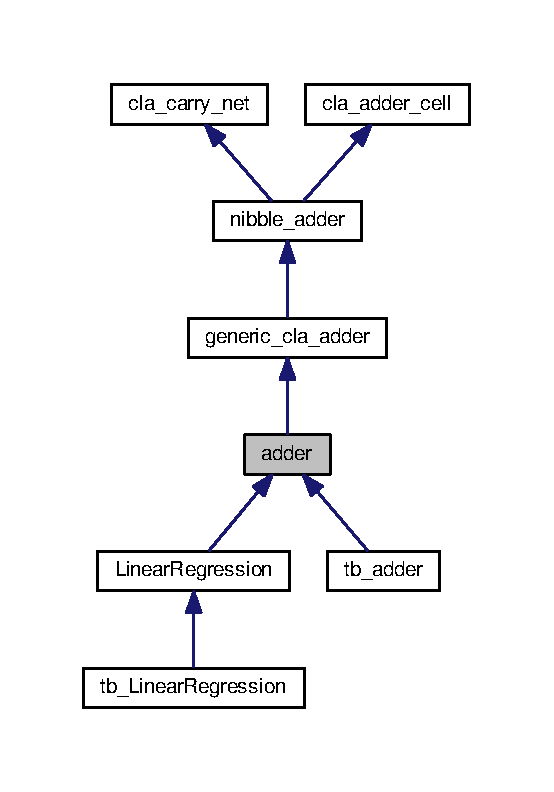
\includegraphics[width=259pt]{classadder__inherit__graph}
\end{center}
\end{figure}


Diagramma di collaborazione per adder\+:\nopagebreak
\begin{figure}[H]
\begin{center}
\leavevmode
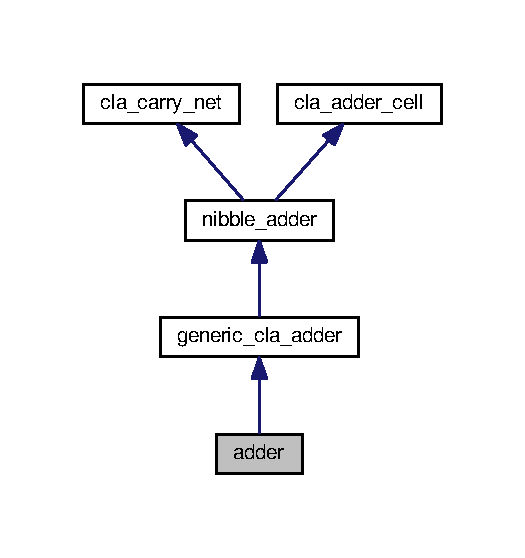
\includegraphics[width=252pt]{classadder__coll__graph}
\end{center}
\end{figure}
\subsection*{Entities}
\begin{DoxyCompactItemize}
\item 
\hyperlink{classadder_1_1structural}{structural} architecture
\begin{DoxyCompactList}\small\item\em Implementazione mista structural per l\textquotesingle{}entity adder.

A seconda del valore del parametro use\+\_\+custom, verrà istanziato
\begin{DoxyItemize}
\item un sommatore full-\/custom \hyperlink{classgeneric__cla__adder}{generic\+\_\+cla\+\_\+adder}, se use\+\_\+custom = true;
\item un sommatore la cui implementazione è stabilita dal sintetizzatore, se use\+\_\+custom = false; Nel caso in cui venga istanziato il sommatore custom, è richiesto che il numero di bit con il quale sono espressi gli addendi, e di conseguenza quello in vui verrà espressa la loro somma, sia multiplo di quattro. 
\end{DoxyItemize}\end{DoxyCompactList}\end{DoxyCompactItemize}
\subsection*{Generics}
 \begin{DoxyCompactItemize}
\item 
\hyperlink{group___adder_gae1435c07d0cd54b521535e2f8de6f94e}{nbits} {\bfseries {\bfseries \textcolor{vhdlchar}{natural}\textcolor{vhdlchar}{ }\textcolor{vhdlchar}{ }\textcolor{vhdlchar}{\+:}\textcolor{vhdlchar}{=}\textcolor{vhdlchar}{ }\textcolor{vhdlchar}{ } \textcolor{vhdldigit}{32} \textcolor{vhdlchar}{ }}}
\item 
\hyperlink{group___adder_gadf05ca347ec6d3c85740dc697469b3db}{use\+\_\+custom} {\bfseries {\bfseries \textcolor{vhdlchar}{boolean}\textcolor{vhdlchar}{ }\textcolor{vhdlchar}{ }\textcolor{vhdlchar}{\+:}\textcolor{vhdlchar}{=}\textcolor{vhdlchar}{ }\textcolor{vhdlchar}{ }\textcolor{vhdlchar}{ }\textcolor{vhdlchar}{ }\textcolor{vhdlchar}{false}\textcolor{vhdlchar}{ }}}
\end{DoxyCompactItemize}
\subsection*{Ports}
 \begin{DoxyCompactItemize}
\item 
\hyperlink{group___adder_gad6ed6073f8ded668a403a0f7d85c53e8}{add1}  {\bfseries {\bfseries \textcolor{vhdlchar}{in}\textcolor{vhdlchar}{ }}} {\bfseries \textcolor{vhdlchar}{std\+\_\+logic\+\_\+vector}\textcolor{vhdlchar}{ }\textcolor{vhdlchar}{(}\textcolor{vhdlchar}{ }\textcolor{vhdlchar}{ }\textcolor{vhdlchar}{ }\textcolor{vhdlchar}{ }{\bfseries \hyperlink{group___adder_gae1435c07d0cd54b521535e2f8de6f94e}{nbits}} \textcolor{vhdlchar}{-\/}\textcolor{vhdlchar}{ } \textcolor{vhdldigit}{1} \textcolor{vhdlchar}{ }\textcolor{vhdlchar}{downto}\textcolor{vhdlchar}{ }\textcolor{vhdlchar}{ } \textcolor{vhdldigit}{0} \textcolor{vhdlchar}{ }\textcolor{vhdlchar}{)}\textcolor{vhdlchar}{ }} 
\begin{DoxyCompactList}\small\item\em addendo 1 \end{DoxyCompactList}\item 
\hyperlink{group___adder_gabf87ad241134c4d313c708910677575e}{add2}  {\bfseries {\bfseries \textcolor{vhdlchar}{in}\textcolor{vhdlchar}{ }}} {\bfseries \textcolor{vhdlchar}{std\+\_\+logic\+\_\+vector}\textcolor{vhdlchar}{ }\textcolor{vhdlchar}{(}\textcolor{vhdlchar}{ }\textcolor{vhdlchar}{ }\textcolor{vhdlchar}{ }\textcolor{vhdlchar}{ }{\bfseries \hyperlink{group___adder_gae1435c07d0cd54b521535e2f8de6f94e}{nbits}} \textcolor{vhdlchar}{-\/}\textcolor{vhdlchar}{ } \textcolor{vhdldigit}{1} \textcolor{vhdlchar}{ }\textcolor{vhdlchar}{downto}\textcolor{vhdlchar}{ }\textcolor{vhdlchar}{ } \textcolor{vhdldigit}{0} \textcolor{vhdlchar}{ }\textcolor{vhdlchar}{)}\textcolor{vhdlchar}{ }} 
\begin{DoxyCompactList}\small\item\em addendo 2 \end{DoxyCompactList}\item 
\hyperlink{group___adder_ga01f6ea3ddb4d1519676217bcb5959de8}{sum}  {\bfseries {\bfseries \textcolor{vhdlchar}{out}\textcolor{vhdlchar}{ }}} {\bfseries \textcolor{vhdlchar}{std\+\_\+logic\+\_\+vector}\textcolor{vhdlchar}{ }\textcolor{vhdlchar}{(}\textcolor{vhdlchar}{ }\textcolor{vhdlchar}{ }\textcolor{vhdlchar}{ }\textcolor{vhdlchar}{ }{\bfseries \hyperlink{group___adder_gae1435c07d0cd54b521535e2f8de6f94e}{nbits}} \textcolor{vhdlchar}{-\/}\textcolor{vhdlchar}{ } \textcolor{vhdldigit}{1} \textcolor{vhdlchar}{ }\textcolor{vhdlchar}{downto}\textcolor{vhdlchar}{ }\textcolor{vhdlchar}{ } \textcolor{vhdldigit}{0} \textcolor{vhdlchar}{ }\textcolor{vhdlchar}{)}\textcolor{vhdlchar}{ }} 
\begin{DoxyCompactList}\small\item\em somma degli addendi \end{DoxyCompactList}\item 
\hyperlink{group___adder_ga9650307dde287e0bcfa1e26370c006c2}{overflow}  {\bfseries {\bfseries \textcolor{vhdlchar}{out}\textcolor{vhdlchar}{ }}} {\bfseries \textcolor{vhdlchar}{std\+\_\+logic}\textcolor{vhdlchar}{ }} 
\end{DoxyCompactItemize}


\subsection{Descrizione dettagliata}
Sommatore a due addendi.

Il sommatore permette di effettuare una somma di due addendi espressi su un certo numero di bit. La somma dei due addendi viene espressa sullo stesso numero di bit. Quando il risultato prodotto dalla somma degli addendi non è correttamente rappresentato su tale numero di bit, un flag indica la condizione di overflow. 

La documentazione per questa classe è stata generata a partire dal seguente file\+:\begin{DoxyCompactItemize}
\item 
Src/adder/\hyperlink{adder_8vhd}{adder.\+vhd}\end{DoxyCompactItemize}

\hypertarget{classtb__adder_1_1behavior}{}\section{behavior Architecture Reference}
\label{classtb__adder_1_1behavior}\index{behavior@{behavior}}
\subsection*{Processes}
 \begin{DoxyCompactItemize}
\item 
\hyperlink{classtb__adder_1_1behavior_ad2efa6785cff833c341e27596b21aeb5}{stim\+\_\+proc}{\bfseries  (  )}
\end{DoxyCompactItemize}
\subsection*{Components}
 \begin{DoxyCompactItemize}
\item 
\hyperlink{classtb__adder_1_1behavior_a9d7a8a381439c61aea549e7a47ec7a6f}{adder}  {\bfseries }  
\end{DoxyCompactItemize}
\subsection*{Constants}
 \begin{DoxyCompactItemize}
\item 
\hyperlink{classtb__adder_1_1behavior_aff8823a253db156c5a7a40d1b813343f}{nbits} {\bfseries \textcolor{vhdlchar}{natural}\textcolor{vhdlchar}{ }\textcolor{vhdlchar}{ }\textcolor{vhdlchar}{\+:}\textcolor{vhdlchar}{=}\textcolor{vhdlchar}{ }\textcolor{vhdlchar}{ } \textcolor{vhdldigit}{12} \textcolor{vhdlchar}{ }} 
\item 
\hyperlink{classtb__adder_1_1behavior_ae53b6cfbb1b5d32c932c417636d6ac3c}{use\+\_\+custom} {\bfseries \textcolor{vhdlchar}{boolean}\textcolor{vhdlchar}{ }\textcolor{vhdlchar}{ }\textcolor{vhdlchar}{\+:}\textcolor{vhdlchar}{=}\textcolor{vhdlchar}{ }\textcolor{vhdlchar}{ }\textcolor{vhdlchar}{ }\textcolor{vhdlchar}{ }\textcolor{vhdlchar}{true}\textcolor{vhdlchar}{ }} 
\end{DoxyCompactItemize}
\subsection*{Signals}
 \begin{DoxyCompactItemize}
\item 
\hyperlink{classtb__adder_1_1behavior_a1c7a41b72844f6ed4f7cf1ab81102a2a}{add1} {\bfseries \textcolor{vhdlchar}{std\+\_\+logic\+\_\+vector}\textcolor{vhdlchar}{ }\textcolor{vhdlchar}{(}\textcolor{vhdlchar}{ }\textcolor{vhdlchar}{ }\textcolor{vhdlchar}{ }\textcolor{vhdlchar}{ }{\bfseries \hyperlink{classtb__adder_1_1behavior_aff8823a253db156c5a7a40d1b813343f}{nbits}} \textcolor{vhdlchar}{-\/}\textcolor{vhdlchar}{ } \textcolor{vhdldigit}{1} \textcolor{vhdlchar}{ }\textcolor{vhdlchar}{downto}\textcolor{vhdlchar}{ }\textcolor{vhdlchar}{ } \textcolor{vhdldigit}{0} \textcolor{vhdlchar}{ }\textcolor{vhdlchar}{)}\textcolor{vhdlchar}{ }\textcolor{vhdlchar}{ }\textcolor{vhdlchar}{ }\textcolor{vhdlchar}{\+:}\textcolor{vhdlchar}{=}\textcolor{vhdlchar}{ }\textcolor{vhdlchar}{(}\textcolor{vhdlchar}{ }\textcolor{vhdlchar}{ }\textcolor{vhdlchar}{others}\textcolor{vhdlchar}{ }\textcolor{vhdlchar}{ }\textcolor{vhdlchar}{=}\textcolor{vhdlchar}{ }\textcolor{vhdlchar}{$>$}\textcolor{vhdlchar}{ }\textcolor{vhdlchar}{\textquotesingle{}}\textcolor{vhdlchar}{ } \textcolor{vhdldigit}{0} \textcolor{vhdlchar}{ }\textcolor{vhdlchar}{\textquotesingle{}}\textcolor{vhdlchar}{ }\textcolor{vhdlchar}{)}\textcolor{vhdlchar}{ }} 
\item 
\hyperlink{classtb__adder_1_1behavior_aa713d21db1284f6652f7e63e60cacaa1}{add2} {\bfseries \textcolor{vhdlchar}{std\+\_\+logic\+\_\+vector}\textcolor{vhdlchar}{ }\textcolor{vhdlchar}{(}\textcolor{vhdlchar}{ }\textcolor{vhdlchar}{ }\textcolor{vhdlchar}{ }\textcolor{vhdlchar}{ }{\bfseries \hyperlink{classtb__adder_1_1behavior_aff8823a253db156c5a7a40d1b813343f}{nbits}} \textcolor{vhdlchar}{-\/}\textcolor{vhdlchar}{ } \textcolor{vhdldigit}{1} \textcolor{vhdlchar}{ }\textcolor{vhdlchar}{downto}\textcolor{vhdlchar}{ }\textcolor{vhdlchar}{ } \textcolor{vhdldigit}{0} \textcolor{vhdlchar}{ }\textcolor{vhdlchar}{)}\textcolor{vhdlchar}{ }\textcolor{vhdlchar}{ }\textcolor{vhdlchar}{ }\textcolor{vhdlchar}{\+:}\textcolor{vhdlchar}{=}\textcolor{vhdlchar}{ }\textcolor{vhdlchar}{(}\textcolor{vhdlchar}{ }\textcolor{vhdlchar}{ }\textcolor{vhdlchar}{others}\textcolor{vhdlchar}{ }\textcolor{vhdlchar}{ }\textcolor{vhdlchar}{=}\textcolor{vhdlchar}{ }\textcolor{vhdlchar}{$>$}\textcolor{vhdlchar}{ }\textcolor{vhdlchar}{\textquotesingle{}}\textcolor{vhdlchar}{ } \textcolor{vhdldigit}{0} \textcolor{vhdlchar}{ }\textcolor{vhdlchar}{\textquotesingle{}}\textcolor{vhdlchar}{ }\textcolor{vhdlchar}{)}\textcolor{vhdlchar}{ }} 
\item 
\hyperlink{classtb__adder_1_1behavior_a5db139547621616405be3e820278d444}{sum} {\bfseries \textcolor{vhdlchar}{std\+\_\+logic\+\_\+vector}\textcolor{vhdlchar}{ }\textcolor{vhdlchar}{(}\textcolor{vhdlchar}{ }\textcolor{vhdlchar}{ }\textcolor{vhdlchar}{ }\textcolor{vhdlchar}{ }{\bfseries \hyperlink{classtb__adder_1_1behavior_aff8823a253db156c5a7a40d1b813343f}{nbits}} \textcolor{vhdlchar}{-\/}\textcolor{vhdlchar}{ } \textcolor{vhdldigit}{1} \textcolor{vhdlchar}{ }\textcolor{vhdlchar}{downto}\textcolor{vhdlchar}{ }\textcolor{vhdlchar}{ } \textcolor{vhdldigit}{0} \textcolor{vhdlchar}{ }\textcolor{vhdlchar}{)}\textcolor{vhdlchar}{ }\textcolor{vhdlchar}{ }\textcolor{vhdlchar}{ }\textcolor{vhdlchar}{\+:}\textcolor{vhdlchar}{=}\textcolor{vhdlchar}{ }\textcolor{vhdlchar}{(}\textcolor{vhdlchar}{ }\textcolor{vhdlchar}{ }\textcolor{vhdlchar}{others}\textcolor{vhdlchar}{ }\textcolor{vhdlchar}{ }\textcolor{vhdlchar}{=}\textcolor{vhdlchar}{ }\textcolor{vhdlchar}{$>$}\textcolor{vhdlchar}{ }\textcolor{vhdlchar}{\textquotesingle{}}\textcolor{vhdlchar}{ } \textcolor{vhdldigit}{0} \textcolor{vhdlchar}{ }\textcolor{vhdlchar}{\textquotesingle{}}\textcolor{vhdlchar}{ }\textcolor{vhdlchar}{)}\textcolor{vhdlchar}{ }} 
\item 
\hyperlink{classtb__adder_1_1behavior_ab579763af0d4bea3c24be9431798eeea}{overflow} {\bfseries \textcolor{vhdlchar}{std\+\_\+logic}\textcolor{vhdlchar}{ }\textcolor{vhdlchar}{ }\textcolor{vhdlchar}{\+:}\textcolor{vhdlchar}{=}\textcolor{vhdlchar}{ }\textcolor{vhdlchar}{ }\textcolor{vhdlchar}{\textquotesingle{}}\textcolor{vhdlchar}{ } \textcolor{vhdldigit}{0} \textcolor{vhdlchar}{ }\textcolor{vhdlchar}{\textquotesingle{}}\textcolor{vhdlchar}{ }} 
\end{DoxyCompactItemize}
\subsection*{Instantiations}
 \begin{DoxyCompactItemize}
\item 
\hyperlink{classtb__adder_1_1behavior_a1619316ad715601eb5d3559db829ac05}{uut}  {\bfseries adder}   
\end{DoxyCompactItemize}


\subsection{Documentazione delle funzioni membro}
\mbox{\Hypertarget{classtb__adder_1_1behavior_ad2efa6785cff833c341e27596b21aeb5}\label{classtb__adder_1_1behavior_ad2efa6785cff833c341e27596b21aeb5}} 
\index{tb\+\_\+adder\+::behavior@{tb\+\_\+adder\+::behavior}!stim\+\_\+proc@{stim\+\_\+proc}}
\index{stim\+\_\+proc@{stim\+\_\+proc}!tb\+\_\+adder\+::behavior@{tb\+\_\+adder\+::behavior}}
\subsubsection{\texorpdfstring{stim\+\_\+proc()}{stim\_proc()}}
{\footnotesize\ttfamily stim\+\_\+proc (\begin{DoxyParamCaption}{ }\end{DoxyParamCaption})}



\subsection{Documentazione dei membri dato}
\mbox{\Hypertarget{classtb__adder_1_1behavior_a1c7a41b72844f6ed4f7cf1ab81102a2a}\label{classtb__adder_1_1behavior_a1c7a41b72844f6ed4f7cf1ab81102a2a}} 
\index{tb\+\_\+adder\+::behavior@{tb\+\_\+adder\+::behavior}!add1@{add1}}
\index{add1@{add1}!tb\+\_\+adder\+::behavior@{tb\+\_\+adder\+::behavior}}
\subsubsection{\texorpdfstring{add1}{add1}}
{\footnotesize\ttfamily \hyperlink{classtb__adder_1_1behavior_a1c7a41b72844f6ed4f7cf1ab81102a2a}{add1} {\bfseries \textcolor{vhdlchar}{std\+\_\+logic\+\_\+vector}\textcolor{vhdlchar}{ }\textcolor{vhdlchar}{(}\textcolor{vhdlchar}{ }\textcolor{vhdlchar}{ }\textcolor{vhdlchar}{ }\textcolor{vhdlchar}{ }{\bfseries \hyperlink{classtb__adder_1_1behavior_aff8823a253db156c5a7a40d1b813343f}{nbits}} \textcolor{vhdlchar}{-\/}\textcolor{vhdlchar}{ } \textcolor{vhdldigit}{1} \textcolor{vhdlchar}{ }\textcolor{vhdlchar}{downto}\textcolor{vhdlchar}{ }\textcolor{vhdlchar}{ } \textcolor{vhdldigit}{0} \textcolor{vhdlchar}{ }\textcolor{vhdlchar}{)}\textcolor{vhdlchar}{ }\textcolor{vhdlchar}{ }\textcolor{vhdlchar}{ }\textcolor{vhdlchar}{\+:}\textcolor{vhdlchar}{=}\textcolor{vhdlchar}{ }\textcolor{vhdlchar}{(}\textcolor{vhdlchar}{ }\textcolor{vhdlchar}{ }\textcolor{vhdlchar}{others}\textcolor{vhdlchar}{ }\textcolor{vhdlchar}{ }\textcolor{vhdlchar}{=}\textcolor{vhdlchar}{ }\textcolor{vhdlchar}{$>$}\textcolor{vhdlchar}{ }\textcolor{vhdlchar}{\textquotesingle{}}\textcolor{vhdlchar}{ } \textcolor{vhdldigit}{0} \textcolor{vhdlchar}{ }\textcolor{vhdlchar}{\textquotesingle{}}\textcolor{vhdlchar}{ }\textcolor{vhdlchar}{)}\textcolor{vhdlchar}{ }} \hspace{0.3cm}{\ttfamily [Signal]}}

\mbox{\Hypertarget{classtb__adder_1_1behavior_aa713d21db1284f6652f7e63e60cacaa1}\label{classtb__adder_1_1behavior_aa713d21db1284f6652f7e63e60cacaa1}} 
\index{tb\+\_\+adder\+::behavior@{tb\+\_\+adder\+::behavior}!add2@{add2}}
\index{add2@{add2}!tb\+\_\+adder\+::behavior@{tb\+\_\+adder\+::behavior}}
\subsubsection{\texorpdfstring{add2}{add2}}
{\footnotesize\ttfamily \hyperlink{classtb__adder_1_1behavior_aa713d21db1284f6652f7e63e60cacaa1}{add2} {\bfseries \textcolor{vhdlchar}{std\+\_\+logic\+\_\+vector}\textcolor{vhdlchar}{ }\textcolor{vhdlchar}{(}\textcolor{vhdlchar}{ }\textcolor{vhdlchar}{ }\textcolor{vhdlchar}{ }\textcolor{vhdlchar}{ }{\bfseries \hyperlink{classtb__adder_1_1behavior_aff8823a253db156c5a7a40d1b813343f}{nbits}} \textcolor{vhdlchar}{-\/}\textcolor{vhdlchar}{ } \textcolor{vhdldigit}{1} \textcolor{vhdlchar}{ }\textcolor{vhdlchar}{downto}\textcolor{vhdlchar}{ }\textcolor{vhdlchar}{ } \textcolor{vhdldigit}{0} \textcolor{vhdlchar}{ }\textcolor{vhdlchar}{)}\textcolor{vhdlchar}{ }\textcolor{vhdlchar}{ }\textcolor{vhdlchar}{ }\textcolor{vhdlchar}{\+:}\textcolor{vhdlchar}{=}\textcolor{vhdlchar}{ }\textcolor{vhdlchar}{(}\textcolor{vhdlchar}{ }\textcolor{vhdlchar}{ }\textcolor{vhdlchar}{others}\textcolor{vhdlchar}{ }\textcolor{vhdlchar}{ }\textcolor{vhdlchar}{=}\textcolor{vhdlchar}{ }\textcolor{vhdlchar}{$>$}\textcolor{vhdlchar}{ }\textcolor{vhdlchar}{\textquotesingle{}}\textcolor{vhdlchar}{ } \textcolor{vhdldigit}{0} \textcolor{vhdlchar}{ }\textcolor{vhdlchar}{\textquotesingle{}}\textcolor{vhdlchar}{ }\textcolor{vhdlchar}{)}\textcolor{vhdlchar}{ }} \hspace{0.3cm}{\ttfamily [Signal]}}

\mbox{\Hypertarget{classtb__adder_1_1behavior_a9d7a8a381439c61aea549e7a47ec7a6f}\label{classtb__adder_1_1behavior_a9d7a8a381439c61aea549e7a47ec7a6f}} 
\index{tb\+\_\+adder\+::behavior@{tb\+\_\+adder\+::behavior}!adder@{adder}}
\index{adder@{adder}!tb\+\_\+adder\+::behavior@{tb\+\_\+adder\+::behavior}}
\subsubsection{\texorpdfstring{adder}{adder}}
{\footnotesize\ttfamily \hyperlink{classtb__adder_1_1behavior_a9d7a8a381439c61aea549e7a47ec7a6f}{adder} {\bfseries \textcolor{vhdlchar}{ }} \hspace{0.3cm}{\ttfamily [Component]}}

\mbox{\Hypertarget{classtb__adder_1_1behavior_aff8823a253db156c5a7a40d1b813343f}\label{classtb__adder_1_1behavior_aff8823a253db156c5a7a40d1b813343f}} 
\index{tb\+\_\+adder\+::behavior@{tb\+\_\+adder\+::behavior}!nbits@{nbits}}
\index{nbits@{nbits}!tb\+\_\+adder\+::behavior@{tb\+\_\+adder\+::behavior}}
\subsubsection{\texorpdfstring{nbits}{nbits}}
{\footnotesize\ttfamily \hyperlink{classtb__adder_1_1behavior_aff8823a253db156c5a7a40d1b813343f}{nbits} {\bfseries \textcolor{vhdlchar}{natural}\textcolor{vhdlchar}{ }\textcolor{vhdlchar}{ }\textcolor{vhdlchar}{\+:}\textcolor{vhdlchar}{=}\textcolor{vhdlchar}{ }\textcolor{vhdlchar}{ } \textcolor{vhdldigit}{12} \textcolor{vhdlchar}{ }} \hspace{0.3cm}{\ttfamily [Constant]}}

\mbox{\Hypertarget{classtb__adder_1_1behavior_ab579763af0d4bea3c24be9431798eeea}\label{classtb__adder_1_1behavior_ab579763af0d4bea3c24be9431798eeea}} 
\index{tb\+\_\+adder\+::behavior@{tb\+\_\+adder\+::behavior}!overflow@{overflow}}
\index{overflow@{overflow}!tb\+\_\+adder\+::behavior@{tb\+\_\+adder\+::behavior}}
\subsubsection{\texorpdfstring{overflow}{overflow}}
{\footnotesize\ttfamily \hyperlink{classtb__adder_1_1behavior_ab579763af0d4bea3c24be9431798eeea}{overflow} {\bfseries \textcolor{vhdlchar}{std\+\_\+logic}\textcolor{vhdlchar}{ }\textcolor{vhdlchar}{ }\textcolor{vhdlchar}{\+:}\textcolor{vhdlchar}{=}\textcolor{vhdlchar}{ }\textcolor{vhdlchar}{ }\textcolor{vhdlchar}{\textquotesingle{}}\textcolor{vhdlchar}{ } \textcolor{vhdldigit}{0} \textcolor{vhdlchar}{ }\textcolor{vhdlchar}{\textquotesingle{}}\textcolor{vhdlchar}{ }} \hspace{0.3cm}{\ttfamily [Signal]}}

\mbox{\Hypertarget{classtb__adder_1_1behavior_a5db139547621616405be3e820278d444}\label{classtb__adder_1_1behavior_a5db139547621616405be3e820278d444}} 
\index{tb\+\_\+adder\+::behavior@{tb\+\_\+adder\+::behavior}!sum@{sum}}
\index{sum@{sum}!tb\+\_\+adder\+::behavior@{tb\+\_\+adder\+::behavior}}
\subsubsection{\texorpdfstring{sum}{sum}}
{\footnotesize\ttfamily \hyperlink{classtb__adder_1_1behavior_a5db139547621616405be3e820278d444}{sum} {\bfseries \textcolor{vhdlchar}{std\+\_\+logic\+\_\+vector}\textcolor{vhdlchar}{ }\textcolor{vhdlchar}{(}\textcolor{vhdlchar}{ }\textcolor{vhdlchar}{ }\textcolor{vhdlchar}{ }\textcolor{vhdlchar}{ }{\bfseries \hyperlink{classtb__adder_1_1behavior_aff8823a253db156c5a7a40d1b813343f}{nbits}} \textcolor{vhdlchar}{-\/}\textcolor{vhdlchar}{ } \textcolor{vhdldigit}{1} \textcolor{vhdlchar}{ }\textcolor{vhdlchar}{downto}\textcolor{vhdlchar}{ }\textcolor{vhdlchar}{ } \textcolor{vhdldigit}{0} \textcolor{vhdlchar}{ }\textcolor{vhdlchar}{)}\textcolor{vhdlchar}{ }\textcolor{vhdlchar}{ }\textcolor{vhdlchar}{ }\textcolor{vhdlchar}{\+:}\textcolor{vhdlchar}{=}\textcolor{vhdlchar}{ }\textcolor{vhdlchar}{(}\textcolor{vhdlchar}{ }\textcolor{vhdlchar}{ }\textcolor{vhdlchar}{others}\textcolor{vhdlchar}{ }\textcolor{vhdlchar}{ }\textcolor{vhdlchar}{=}\textcolor{vhdlchar}{ }\textcolor{vhdlchar}{$>$}\textcolor{vhdlchar}{ }\textcolor{vhdlchar}{\textquotesingle{}}\textcolor{vhdlchar}{ } \textcolor{vhdldigit}{0} \textcolor{vhdlchar}{ }\textcolor{vhdlchar}{\textquotesingle{}}\textcolor{vhdlchar}{ }\textcolor{vhdlchar}{)}\textcolor{vhdlchar}{ }} \hspace{0.3cm}{\ttfamily [Signal]}}

\mbox{\Hypertarget{classtb__adder_1_1behavior_ae53b6cfbb1b5d32c932c417636d6ac3c}\label{classtb__adder_1_1behavior_ae53b6cfbb1b5d32c932c417636d6ac3c}} 
\index{tb\+\_\+adder\+::behavior@{tb\+\_\+adder\+::behavior}!use\+\_\+custom@{use\+\_\+custom}}
\index{use\+\_\+custom@{use\+\_\+custom}!tb\+\_\+adder\+::behavior@{tb\+\_\+adder\+::behavior}}
\subsubsection{\texorpdfstring{use\+\_\+custom}{use\_custom}}
{\footnotesize\ttfamily \hyperlink{classtb__adder_1_1behavior_ae53b6cfbb1b5d32c932c417636d6ac3c}{use\+\_\+custom} {\bfseries \textcolor{vhdlchar}{boolean}\textcolor{vhdlchar}{ }\textcolor{vhdlchar}{ }\textcolor{vhdlchar}{\+:}\textcolor{vhdlchar}{=}\textcolor{vhdlchar}{ }\textcolor{vhdlchar}{ }\textcolor{vhdlchar}{ }\textcolor{vhdlchar}{ }\textcolor{vhdlchar}{true}\textcolor{vhdlchar}{ }} \hspace{0.3cm}{\ttfamily [Constant]}}

\mbox{\Hypertarget{classtb__adder_1_1behavior_a1619316ad715601eb5d3559db829ac05}\label{classtb__adder_1_1behavior_a1619316ad715601eb5d3559db829ac05}} 
\index{tb\+\_\+adder\+::behavior@{tb\+\_\+adder\+::behavior}!uut@{uut}}
\index{uut@{uut}!tb\+\_\+adder\+::behavior@{tb\+\_\+adder\+::behavior}}
\subsubsection{\texorpdfstring{uut}{uut}}
{\footnotesize\ttfamily \hyperlink{classtb__adder_1_1behavior_a1619316ad715601eb5d3559db829ac05}{uut} {\bfseries \textcolor{vhdlchar}{adder}\textcolor{vhdlchar}{ }} \hspace{0.3cm}{\ttfamily [Instantiation]}}



La documentazione per questa classe è stata generata a partire dal seguente file\+:\begin{DoxyCompactItemize}
\item 
Src/adder/\hyperlink{tb__adder_8vhd}{tb\+\_\+adder.\+vhd}\end{DoxyCompactItemize}

\hypertarget{classtb__generic__cla__adder_1_1behavior}{\section{behavior Architecture Reference}
\label{classtb__generic__cla__adder_1_1behavior}\index{behavior@{behavior}}
}
\subsection*{Processes}
 \begin{DoxyCompactItemize}
\item 
\hyperlink{classtb__generic__cla__adder_1_1behavior_ad2efa6785cff833c341e27596b21aeb5}{stim\+\_\+proc}{\bfseries  (  )}
\end{DoxyCompactItemize}
\subsection*{Components}
 \begin{DoxyCompactItemize}
\item 
\hyperlink{classtb__generic__cla__adder_1_1behavior_ae7148956d4ef1d1cd14f35060634b9c3}{generic\+\_\+cla\+\_\+adder}  {\bfseries }  
\end{DoxyCompactItemize}
\subsection*{Signals}
 \begin{DoxyCompactItemize}
\item 
\hyperlink{classtb__generic__cla__adder_1_1behavior_a674dc264b83bd397c51160bed4eaede8}{carry\+\_\+in} {\bfseries \textcolor{vhdlchar}{std\+\_\+logic}\textcolor{vhdlchar}{ }\textcolor{vhdlchar}{ }\textcolor{vhdlchar}{\+:}\textcolor{vhdlchar}{=}\textcolor{vhdlchar}{ }\textcolor{vhdlchar}{ }\textcolor{vhdlchar}{'}\textcolor{vhdlchar}{ } \textcolor{vhdldigit}{0} \textcolor{vhdlchar}{ }\textcolor{vhdlchar}{'}\textcolor{vhdlchar}{ }} 
\item 
\hyperlink{classtb__generic__cla__adder_1_1behavior_a60ae79202e8be952cf4f6d017cc743f1}{X} {\bfseries \textcolor{vhdlchar}{std\+\_\+logic\+\_\+vector}\textcolor{vhdlchar}{ }\textcolor{vhdlchar}{(}\textcolor{vhdlchar}{ }\textcolor{vhdlchar}{ } \textcolor{vhdldigit}{7} \textcolor{vhdlchar}{ }\textcolor{vhdlchar}{downto}\textcolor{vhdlchar}{ }\textcolor{vhdlchar}{ } \textcolor{vhdldigit}{0} \textcolor{vhdlchar}{ }\textcolor{vhdlchar}{)}\textcolor{vhdlchar}{ }\textcolor{vhdlchar}{ }\textcolor{vhdlchar}{ }\textcolor{vhdlchar}{\+:}\textcolor{vhdlchar}{=}\textcolor{vhdlchar}{ }\textcolor{vhdlchar}{(}\textcolor{vhdlchar}{ }\textcolor{vhdlchar}{ }\textcolor{vhdlchar}{others}\textcolor{vhdlchar}{ }\textcolor{vhdlchar}{ }\textcolor{vhdlchar}{=}\textcolor{vhdlchar}{ }\textcolor{vhdlchar}{$>$}\textcolor{vhdlchar}{ }\textcolor{vhdlchar}{'}\textcolor{vhdlchar}{ } \textcolor{vhdldigit}{0} \textcolor{vhdlchar}{ }\textcolor{vhdlchar}{'}\textcolor{vhdlchar}{ }\textcolor{vhdlchar}{)}\textcolor{vhdlchar}{ }} 
\item 
\hyperlink{classtb__generic__cla__adder_1_1behavior_a90a36bc161877c328423b965fab6bd93}{Y} {\bfseries \textcolor{vhdlchar}{std\+\_\+logic\+\_\+vector}\textcolor{vhdlchar}{ }\textcolor{vhdlchar}{(}\textcolor{vhdlchar}{ }\textcolor{vhdlchar}{ } \textcolor{vhdldigit}{7} \textcolor{vhdlchar}{ }\textcolor{vhdlchar}{downto}\textcolor{vhdlchar}{ }\textcolor{vhdlchar}{ } \textcolor{vhdldigit}{0} \textcolor{vhdlchar}{ }\textcolor{vhdlchar}{)}\textcolor{vhdlchar}{ }\textcolor{vhdlchar}{ }\textcolor{vhdlchar}{ }\textcolor{vhdlchar}{\+:}\textcolor{vhdlchar}{=}\textcolor{vhdlchar}{ }\textcolor{vhdlchar}{(}\textcolor{vhdlchar}{ }\textcolor{vhdlchar}{ }\textcolor{vhdlchar}{others}\textcolor{vhdlchar}{ }\textcolor{vhdlchar}{ }\textcolor{vhdlchar}{=}\textcolor{vhdlchar}{ }\textcolor{vhdlchar}{$>$}\textcolor{vhdlchar}{ }\textcolor{vhdlchar}{'}\textcolor{vhdlchar}{ } \textcolor{vhdldigit}{0} \textcolor{vhdlchar}{ }\textcolor{vhdlchar}{'}\textcolor{vhdlchar}{ }\textcolor{vhdlchar}{)}\textcolor{vhdlchar}{ }} 
\item 
\hyperlink{classtb__generic__cla__adder_1_1behavior_a2f702f7ff5535941ec77a2859f9686b7}{sum} {\bfseries \textcolor{vhdlchar}{std\+\_\+logic\+\_\+vector}\textcolor{vhdlchar}{ }\textcolor{vhdlchar}{(}\textcolor{vhdlchar}{ }\textcolor{vhdlchar}{ } \textcolor{vhdldigit}{7} \textcolor{vhdlchar}{ }\textcolor{vhdlchar}{downto}\textcolor{vhdlchar}{ }\textcolor{vhdlchar}{ } \textcolor{vhdldigit}{0} \textcolor{vhdlchar}{ }\textcolor{vhdlchar}{)}\textcolor{vhdlchar}{ }} 
\item 
\hyperlink{classtb__generic__cla__adder_1_1behavior_a0599dd129c582752ab70084bd7bd6305}{carry\+\_\+out} {\bfseries \textcolor{vhdlchar}{std\+\_\+logic}\textcolor{vhdlchar}{ }} 
\end{DoxyCompactItemize}
\subsection*{Instantiations}
 \begin{DoxyCompactItemize}
\item 
\hyperlink{classtb__generic__cla__adder_1_1behavior_a1619316ad715601eb5d3559db829ac05}{uut}  {\bfseries generic\+\_\+cla\+\_\+adder}   
\end{DoxyCompactItemize}


\subsection{Documentazione delle funzioni membro}
\hypertarget{classtb__generic__cla__adder_1_1behavior_ad2efa6785cff833c341e27596b21aeb5}{\index{tb\+\_\+generic\+\_\+cla\+\_\+adder\+::behavior@{tb\+\_\+generic\+\_\+cla\+\_\+adder\+::behavior}!stim\+\_\+proc@{stim\+\_\+proc}}
\index{stim\+\_\+proc@{stim\+\_\+proc}!tb\+\_\+generic\+\_\+cla\+\_\+adder\+::behavior@{tb\+\_\+generic\+\_\+cla\+\_\+adder\+::behavior}}
\subsubsection[{stim\+\_\+proc}]{\setlength{\rightskip}{0pt plus 5cm}stim\+\_\+proc (
\begin{DoxyParamCaption}
{}
\end{DoxyParamCaption}
)}}\label{classtb__generic__cla__adder_1_1behavior_ad2efa6785cff833c341e27596b21aeb5}


\subsection{Documentazione dei membri dato}
\hypertarget{classtb__generic__cla__adder_1_1behavior_a674dc264b83bd397c51160bed4eaede8}{\index{tb\+\_\+generic\+\_\+cla\+\_\+adder\+::behavior@{tb\+\_\+generic\+\_\+cla\+\_\+adder\+::behavior}!carry\+\_\+in@{carry\+\_\+in}}
\index{carry\+\_\+in@{carry\+\_\+in}!tb\+\_\+generic\+\_\+cla\+\_\+adder\+::behavior@{tb\+\_\+generic\+\_\+cla\+\_\+adder\+::behavior}}
\subsubsection[{carry\+\_\+in}]{\setlength{\rightskip}{0pt plus 5cm}{\bf carry\+\_\+in} {\bfseries \textcolor{vhdlchar}{std\+\_\+logic}\textcolor{vhdlchar}{ }\textcolor{vhdlchar}{ }\textcolor{vhdlchar}{\+:}\textcolor{vhdlchar}{=}\textcolor{vhdlchar}{ }\textcolor{vhdlchar}{ }\textcolor{vhdlchar}{'}\textcolor{vhdlchar}{ } \textcolor{vhdldigit}{0} \textcolor{vhdlchar}{ }\textcolor{vhdlchar}{'}\textcolor{vhdlchar}{ }} \hspace{0.3cm}{\ttfamily [Signal]}}}\label{classtb__generic__cla__adder_1_1behavior_a674dc264b83bd397c51160bed4eaede8}
\hypertarget{classtb__generic__cla__adder_1_1behavior_a0599dd129c582752ab70084bd7bd6305}{\index{tb\+\_\+generic\+\_\+cla\+\_\+adder\+::behavior@{tb\+\_\+generic\+\_\+cla\+\_\+adder\+::behavior}!carry\+\_\+out@{carry\+\_\+out}}
\index{carry\+\_\+out@{carry\+\_\+out}!tb\+\_\+generic\+\_\+cla\+\_\+adder\+::behavior@{tb\+\_\+generic\+\_\+cla\+\_\+adder\+::behavior}}
\subsubsection[{carry\+\_\+out}]{\setlength{\rightskip}{0pt plus 5cm}{\bf carry\+\_\+out} {\bfseries \textcolor{vhdlchar}{std\+\_\+logic}\textcolor{vhdlchar}{ }} \hspace{0.3cm}{\ttfamily [Signal]}}}\label{classtb__generic__cla__adder_1_1behavior_a0599dd129c582752ab70084bd7bd6305}
\hypertarget{classtb__generic__cla__adder_1_1behavior_ae7148956d4ef1d1cd14f35060634b9c3}{\index{tb\+\_\+generic\+\_\+cla\+\_\+adder\+::behavior@{tb\+\_\+generic\+\_\+cla\+\_\+adder\+::behavior}!generic\+\_\+cla\+\_\+adder@{generic\+\_\+cla\+\_\+adder}}
\index{generic\+\_\+cla\+\_\+adder@{generic\+\_\+cla\+\_\+adder}!tb\+\_\+generic\+\_\+cla\+\_\+adder\+::behavior@{tb\+\_\+generic\+\_\+cla\+\_\+adder\+::behavior}}
\subsubsection[{generic\+\_\+cla\+\_\+adder}]{\setlength{\rightskip}{0pt plus 5cm}{\bf generic\+\_\+cla\+\_\+adder} {\bfseries \textcolor{vhdlchar}{ }} \hspace{0.3cm}{\ttfamily [Component]}}}\label{classtb__generic__cla__adder_1_1behavior_ae7148956d4ef1d1cd14f35060634b9c3}
\hypertarget{classtb__generic__cla__adder_1_1behavior_a2f702f7ff5535941ec77a2859f9686b7}{\index{tb\+\_\+generic\+\_\+cla\+\_\+adder\+::behavior@{tb\+\_\+generic\+\_\+cla\+\_\+adder\+::behavior}!sum@{sum}}
\index{sum@{sum}!tb\+\_\+generic\+\_\+cla\+\_\+adder\+::behavior@{tb\+\_\+generic\+\_\+cla\+\_\+adder\+::behavior}}
\subsubsection[{sum}]{\setlength{\rightskip}{0pt plus 5cm}{\bf sum} {\bfseries \textcolor{vhdlchar}{std\+\_\+logic\+\_\+vector}\textcolor{vhdlchar}{ }\textcolor{vhdlchar}{(}\textcolor{vhdlchar}{ }\textcolor{vhdlchar}{ } \textcolor{vhdldigit}{7} \textcolor{vhdlchar}{ }\textcolor{vhdlchar}{downto}\textcolor{vhdlchar}{ }\textcolor{vhdlchar}{ } \textcolor{vhdldigit}{0} \textcolor{vhdlchar}{ }\textcolor{vhdlchar}{)}\textcolor{vhdlchar}{ }} \hspace{0.3cm}{\ttfamily [Signal]}}}\label{classtb__generic__cla__adder_1_1behavior_a2f702f7ff5535941ec77a2859f9686b7}
\hypertarget{classtb__generic__cla__adder_1_1behavior_a1619316ad715601eb5d3559db829ac05}{\index{tb\+\_\+generic\+\_\+cla\+\_\+adder\+::behavior@{tb\+\_\+generic\+\_\+cla\+\_\+adder\+::behavior}!uut@{uut}}
\index{uut@{uut}!tb\+\_\+generic\+\_\+cla\+\_\+adder\+::behavior@{tb\+\_\+generic\+\_\+cla\+\_\+adder\+::behavior}}
\subsubsection[{uut}]{\setlength{\rightskip}{0pt plus 5cm}{\bf uut} {\bfseries \textcolor{vhdlchar}{generic\+\_\+cla\+\_\+adder}\textcolor{vhdlchar}{ }} \hspace{0.3cm}{\ttfamily [Instantiation]}}}\label{classtb__generic__cla__adder_1_1behavior_a1619316ad715601eb5d3559db829ac05}
\hypertarget{classtb__generic__cla__adder_1_1behavior_a60ae79202e8be952cf4f6d017cc743f1}{\index{tb\+\_\+generic\+\_\+cla\+\_\+adder\+::behavior@{tb\+\_\+generic\+\_\+cla\+\_\+adder\+::behavior}!X@{X}}
\index{X@{X}!tb\+\_\+generic\+\_\+cla\+\_\+adder\+::behavior@{tb\+\_\+generic\+\_\+cla\+\_\+adder\+::behavior}}
\subsubsection[{X}]{\setlength{\rightskip}{0pt plus 5cm}{\bf X} {\bfseries \textcolor{vhdlchar}{std\+\_\+logic\+\_\+vector}\textcolor{vhdlchar}{ }\textcolor{vhdlchar}{(}\textcolor{vhdlchar}{ }\textcolor{vhdlchar}{ } \textcolor{vhdldigit}{7} \textcolor{vhdlchar}{ }\textcolor{vhdlchar}{downto}\textcolor{vhdlchar}{ }\textcolor{vhdlchar}{ } \textcolor{vhdldigit}{0} \textcolor{vhdlchar}{ }\textcolor{vhdlchar}{)}\textcolor{vhdlchar}{ }\textcolor{vhdlchar}{ }\textcolor{vhdlchar}{ }\textcolor{vhdlchar}{\+:}\textcolor{vhdlchar}{=}\textcolor{vhdlchar}{ }\textcolor{vhdlchar}{(}\textcolor{vhdlchar}{ }\textcolor{vhdlchar}{ }\textcolor{vhdlchar}{others}\textcolor{vhdlchar}{ }\textcolor{vhdlchar}{ }\textcolor{vhdlchar}{=}\textcolor{vhdlchar}{ }\textcolor{vhdlchar}{$>$}\textcolor{vhdlchar}{ }\textcolor{vhdlchar}{'}\textcolor{vhdlchar}{ } \textcolor{vhdldigit}{0} \textcolor{vhdlchar}{ }\textcolor{vhdlchar}{'}\textcolor{vhdlchar}{ }\textcolor{vhdlchar}{)}\textcolor{vhdlchar}{ }} \hspace{0.3cm}{\ttfamily [Signal]}}}\label{classtb__generic__cla__adder_1_1behavior_a60ae79202e8be952cf4f6d017cc743f1}
\hypertarget{classtb__generic__cla__adder_1_1behavior_a90a36bc161877c328423b965fab6bd93}{\index{tb\+\_\+generic\+\_\+cla\+\_\+adder\+::behavior@{tb\+\_\+generic\+\_\+cla\+\_\+adder\+::behavior}!Y@{Y}}
\index{Y@{Y}!tb\+\_\+generic\+\_\+cla\+\_\+adder\+::behavior@{tb\+\_\+generic\+\_\+cla\+\_\+adder\+::behavior}}
\subsubsection[{Y}]{\setlength{\rightskip}{0pt plus 5cm}{\bf Y} {\bfseries \textcolor{vhdlchar}{std\+\_\+logic\+\_\+vector}\textcolor{vhdlchar}{ }\textcolor{vhdlchar}{(}\textcolor{vhdlchar}{ }\textcolor{vhdlchar}{ } \textcolor{vhdldigit}{7} \textcolor{vhdlchar}{ }\textcolor{vhdlchar}{downto}\textcolor{vhdlchar}{ }\textcolor{vhdlchar}{ } \textcolor{vhdldigit}{0} \textcolor{vhdlchar}{ }\textcolor{vhdlchar}{)}\textcolor{vhdlchar}{ }\textcolor{vhdlchar}{ }\textcolor{vhdlchar}{ }\textcolor{vhdlchar}{\+:}\textcolor{vhdlchar}{=}\textcolor{vhdlchar}{ }\textcolor{vhdlchar}{(}\textcolor{vhdlchar}{ }\textcolor{vhdlchar}{ }\textcolor{vhdlchar}{others}\textcolor{vhdlchar}{ }\textcolor{vhdlchar}{ }\textcolor{vhdlchar}{=}\textcolor{vhdlchar}{ }\textcolor{vhdlchar}{$>$}\textcolor{vhdlchar}{ }\textcolor{vhdlchar}{'}\textcolor{vhdlchar}{ } \textcolor{vhdldigit}{0} \textcolor{vhdlchar}{ }\textcolor{vhdlchar}{'}\textcolor{vhdlchar}{ }\textcolor{vhdlchar}{)}\textcolor{vhdlchar}{ }} \hspace{0.3cm}{\ttfamily [Signal]}}}\label{classtb__generic__cla__adder_1_1behavior_a90a36bc161877c328423b965fab6bd93}


La documentazione per questa classe è stata generata a partire dal seguente file\+:\begin{DoxyCompactItemize}
\item 
Src/adder/\hyperlink{tb__generic__cla__adder_8vhd}{tb\+\_\+generic\+\_\+cla\+\_\+adder.\+vhd}\end{DoxyCompactItemize}

\hypertarget{classtb___linear_regression_1_1_behavioral}{}\section{Behavioral Architecture Reference}
\label{classtb___linear_regression_1_1_behavioral}\index{Behavioral@{Behavioral}}
\subsection*{Processes}
 \begin{DoxyCompactItemize}
\item 
\hyperlink{classtb___linear_regression_1_1_behavioral_ac0731c1f0a226305f2a590b4044cdccb}{clock\+\_\+process}{\bfseries  (  )}
\item 
\hyperlink{classtb___linear_regression_1_1_behavioral_ad2efa6785cff833c341e27596b21aeb5}{stim\+\_\+proc}{\bfseries  (  )}
\end{DoxyCompactItemize}
\subsection*{Components}
 \begin{DoxyCompactItemize}
\item 
\hyperlink{classtb___linear_regression_1_1_behavioral_a899499ba78b32b936cd0914831a72c95}{Linear\+Regression}  {\bfseries }  
\end{DoxyCompactItemize}
\subsection*{Instantiations}
 \begin{DoxyCompactItemize}
\item 
\hyperlink{classtb___linear_regression_1_1_behavioral_a1619316ad715601eb5d3559db829ac05}{uut}  {\bfseries Linear\+Regression}   
\end{DoxyCompactItemize}


\subsection{Documentazione delle funzioni membro}
\index{tb\+\_\+\+Linear\+Regression\+::\+Behavioral@{tb\+\_\+\+Linear\+Regression\+::\+Behavioral}!clock\+\_\+process@{clock\+\_\+process}}
\index{clock\+\_\+process@{clock\+\_\+process}!tb\+\_\+\+Linear\+Regression\+::\+Behavioral@{tb\+\_\+\+Linear\+Regression\+::\+Behavioral}}
\subsubsection[{\texorpdfstring{clock\+\_\+process}{clock_process}}]{\setlength{\rightskip}{0pt plus 5cm} {\bfseries \textcolor{vhdlchar}{ }} clock\+\_\+process ( ) \hspace{0.3cm}{\ttfamily [Process]}}\hypertarget{classtb___linear_regression_1_1_behavioral_ac0731c1f0a226305f2a590b4044cdccb}{}\label{classtb___linear_regression_1_1_behavioral_ac0731c1f0a226305f2a590b4044cdccb}
\index{tb\+\_\+\+Linear\+Regression\+::\+Behavioral@{tb\+\_\+\+Linear\+Regression\+::\+Behavioral}!stim\+\_\+proc@{stim\+\_\+proc}}
\index{stim\+\_\+proc@{stim\+\_\+proc}!tb\+\_\+\+Linear\+Regression\+::\+Behavioral@{tb\+\_\+\+Linear\+Regression\+::\+Behavioral}}
\subsubsection[{\texorpdfstring{stim\+\_\+proc}{stim_proc}}]{\setlength{\rightskip}{0pt plus 5cm}stim\+\_\+proc (
\begin{DoxyParamCaption}
{}
\end{DoxyParamCaption}
)}\hypertarget{classtb___linear_regression_1_1_behavioral_ad2efa6785cff833c341e27596b21aeb5}{}\label{classtb___linear_regression_1_1_behavioral_ad2efa6785cff833c341e27596b21aeb5}


\subsection{Documentazione dei membri dato}
\index{tb\+\_\+\+Linear\+Regression\+::\+Behavioral@{tb\+\_\+\+Linear\+Regression\+::\+Behavioral}!Linear\+Regression@{Linear\+Regression}}
\index{Linear\+Regression@{Linear\+Regression}!tb\+\_\+\+Linear\+Regression\+::\+Behavioral@{tb\+\_\+\+Linear\+Regression\+::\+Behavioral}}
\subsubsection[{\texorpdfstring{Linear\+Regression}{LinearRegression}}]{\setlength{\rightskip}{0pt plus 5cm}{\bf Linear\+Regression} {\bfseries \textcolor{vhdlchar}{ }} \hspace{0.3cm}{\ttfamily [Component]}}\hypertarget{classtb___linear_regression_1_1_behavioral_a899499ba78b32b936cd0914831a72c95}{}\label{classtb___linear_regression_1_1_behavioral_a899499ba78b32b936cd0914831a72c95}
\index{tb\+\_\+\+Linear\+Regression\+::\+Behavioral@{tb\+\_\+\+Linear\+Regression\+::\+Behavioral}!uut@{uut}}
\index{uut@{uut}!tb\+\_\+\+Linear\+Regression\+::\+Behavioral@{tb\+\_\+\+Linear\+Regression\+::\+Behavioral}}
\subsubsection[{\texorpdfstring{uut}{uut}}]{\setlength{\rightskip}{0pt plus 5cm}{\bf uut} {\bfseries \textcolor{vhdlchar}{Linear\+Regression}\textcolor{vhdlchar}{ }} \hspace{0.3cm}{\ttfamily [Instantiation]}}\hypertarget{classtb___linear_regression_1_1_behavioral_a1619316ad715601eb5d3559db829ac05}{}\label{classtb___linear_regression_1_1_behavioral_a1619316ad715601eb5d3559db829ac05}


La documentazione per questa classe è stata generata a partire dal seguente file\+:\begin{DoxyCompactItemize}
\item 
Src/testbench/\hyperlink{tb___linear_regression_8vhd}{tb\+\_\+\+Linear\+Regression.\+vhd}\end{DoxyCompactItemize}

\hypertarget{classcla__adder__cell}{}\section{cla\+\_\+adder\+\_\+cell Entity Reference}
\label{classcla__adder__cell}\index{cla\+\_\+adder\+\_\+cell@{cla\+\_\+adder\+\_\+cell}}


Cella base di un addizionatore con carry-\/lookahead.

La cella somma tra loro due addendi ed un carry in ingresso, tutti espressi su un solo bit. Oltre a generare la somma, genera le funzioni \char`\"{}propagazione\char`\"{} e \char`\"{}generazione\char`\"{} del carry.  




Diagramma delle classi per cla\+\_\+adder\+\_\+cell\nopagebreak
\begin{figure}[H]
\begin{center}
\leavevmode
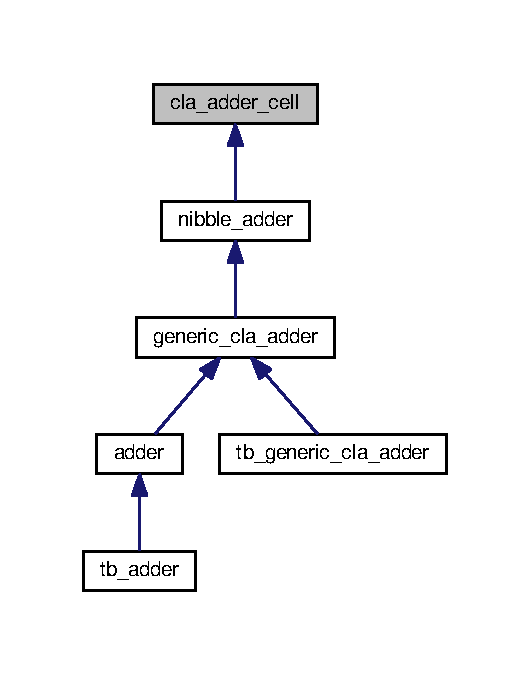
\includegraphics[width=326pt]{classcla__adder__cell__inherit__graph}
\end{center}
\end{figure}
\subsection*{Entities}
\begin{DoxyCompactItemize}
\item 
\hyperlink{classcla__adder__cell_1_1dataflow}{dataflow} architecture
\end{DoxyCompactItemize}
\subsection*{Ports}
 \begin{DoxyCompactItemize}
\item 
\hyperlink{group___base_cell_ga2b16ee1ce0d8ffb8f85ccea13f8ba38d}{add1}  {\bfseries {\bfseries \textcolor{vhdlchar}{in}\textcolor{vhdlchar}{ }}} {\bfseries \textcolor{vhdlchar}{std\+\_\+logic}\textcolor{vhdlchar}{ }} 
\begin{DoxyCompactList}\small\item\em addendo 1 \end{DoxyCompactList}\item 
\hyperlink{group___base_cell_gac3ebb689e34fc5e7657726b18d8b5369}{add2}  {\bfseries {\bfseries \textcolor{vhdlchar}{in}\textcolor{vhdlchar}{ }}} {\bfseries \textcolor{vhdlchar}{std\+\_\+logic}\textcolor{vhdlchar}{ }} 
\begin{DoxyCompactList}\small\item\em addendo 2 \end{DoxyCompactList}\item 
\hyperlink{group___base_cell_gaa556a73dc4a4de1a0d662b25adbcbe33}{carryin}  {\bfseries {\bfseries \textcolor{vhdlchar}{in}\textcolor{vhdlchar}{ }}} {\bfseries \textcolor{vhdlchar}{std\+\_\+logic}\textcolor{vhdlchar}{ }} 
\begin{DoxyCompactList}\small\item\em carry in ingresso \end{DoxyCompactList}\item 
\hyperlink{group___base_cell_gac94466f3a0e3e34f0231abcf4b667ade}{prop}  {\bfseries {\bfseries \textcolor{vhdlchar}{out}\textcolor{vhdlchar}{ }}} {\bfseries \textcolor{vhdlchar}{std\+\_\+logic}\textcolor{vhdlchar}{ }} 
\item 
\hyperlink{group___base_cell_gaad65a9c9ebd4dd83c2835249a1ba2dff}{gen}  {\bfseries {\bfseries \textcolor{vhdlchar}{out}\textcolor{vhdlchar}{ }}} {\bfseries \textcolor{vhdlchar}{std\+\_\+logic}\textcolor{vhdlchar}{ }} 
\item 
\hyperlink{group___base_cell_ga0d9fc1b21b42422b12d68ad73ca8ef13}{sum}  {\bfseries {\bfseries \textcolor{vhdlchar}{out}\textcolor{vhdlchar}{ }}} {\bfseries \textcolor{vhdlchar}{std\+\_\+logic}\textcolor{vhdlchar}{ }} 
\end{DoxyCompactItemize}


\subsection{Descrizione dettagliata}
Cella base di un addizionatore con carry-\/lookahead.

La cella somma tra loro due addendi ed un carry in ingresso, tutti espressi su un solo bit. Oltre a generare la somma, genera le funzioni \char`\"{}propagazione\char`\"{} e \char`\"{}generazione\char`\"{} del carry. 

La documentazione per questa classe è stata generata a partire dal seguente file\+:\begin{DoxyCompactItemize}
\item 
Src/adder/\hyperlink{cla__adder__cell_8vhd}{cla\+\_\+adder\+\_\+cell.\+vhd}\end{DoxyCompactItemize}

\hypertarget{classcla__carry__net}{\section{cla\+\_\+carry\+\_\+net Entity Reference}
\label{classcla__carry__net}\index{cla\+\_\+carry\+\_\+net@{cla\+\_\+carry\+\_\+net}}
}


Rete logica di calcolo dei riporti per un addizionatore a quattro bit con carry lookahead.

Permette di anticipare il calcolo dei riporti usando le funzioni \char`\"{}propagazione\char`\"{} e \char`\"{}generazione\char`\"{} prodotte dai singoli blocchi \hyperlink{classcla__adder__cell}{cla\+\_\+adder\+\_\+cell}, in modo da ridurre tempo necessario ad effettuare il calcolo di tutti i carry, quindi il tempo necessario a completare la somma. Questo blocco calcola solo i carry, pertanto va connesso ai blocchi \hyperlink{classcla__adder__cell}{cla\+\_\+adder\+\_\+cell}, per il calcolo materiale della somma, così come indicato dallo schema seguente, il quale rappresenta lo schema completo di un addizionatore a quattro bit\+: .  




Diagramma delle classi per cla\+\_\+carry\+\_\+net
\nopagebreak
\begin{figure}[H]
\begin{center}
\leavevmode
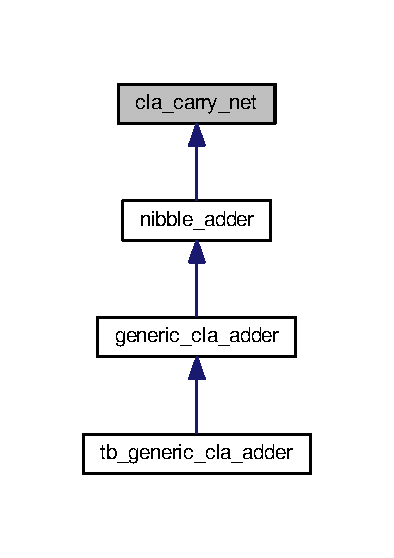
\includegraphics[width=255pt]{classcla__carry__net__inherit__graph}
\end{center}
\end{figure}
\subsection*{Entities}
\begin{DoxyCompactItemize}
\item 
\hyperlink{classcla__carry__net_1_1dataflow}{dataflow} architecture
\begin{DoxyCompactList}\small\item\em Implementazione dataflow dell'entita' \hyperlink{classcla__carry__net}{cla\+\_\+carry\+\_\+net}. \end{DoxyCompactList}\end{DoxyCompactItemize}
\subsection*{Ports}
 \begin{DoxyCompactItemize}
\item 
\hyperlink{group___carry_network_gac1f84cd3374a5a4d2ee2669ebdadafe8}{prop}  {\bfseries {\bfseries \textcolor{vhdlchar}{in}\textcolor{vhdlchar}{ }}} {\bfseries \textcolor{vhdlchar}{std\+\_\+logic\+\_\+vector}\textcolor{vhdlchar}{ }\textcolor{vhdlchar}{(}\textcolor{vhdlchar}{ }\textcolor{vhdlchar}{ } \textcolor{vhdldigit}{3} \textcolor{vhdlchar}{ }\textcolor{vhdlchar}{downto}\textcolor{vhdlchar}{ }\textcolor{vhdlchar}{ } \textcolor{vhdldigit}{0} \textcolor{vhdlchar}{ }\textcolor{vhdlchar}{)}\textcolor{vhdlchar}{ }} 
\begin{DoxyCompactList}\small\item\em funzione “propagazione” prodotta da \hyperlink{classcla__adder__cell}{cla\+\_\+adder\+\_\+cell}; vale 1 quando, sulla base degli ingressi, un adder propaghera' un eventuale carry in ingresso; prop(i) = add(i) O\+R add(i); in questo caso viene prodotta da quattro blocchi \hyperlink{classcla__adder__cell}{cla\+\_\+adder\+\_\+cell} sulla base dei loro ingressi \end{DoxyCompactList}\item 
\hyperlink{group___carry_network_ga1ff97daaf4e03defc21748593cacfaa7}{gen}  {\bfseries {\bfseries \textcolor{vhdlchar}{in}\textcolor{vhdlchar}{ }}} {\bfseries \textcolor{vhdlchar}{std\+\_\+logic\+\_\+vector}\textcolor{vhdlchar}{ }\textcolor{vhdlchar}{(}\textcolor{vhdlchar}{ }\textcolor{vhdlchar}{ } \textcolor{vhdldigit}{3} \textcolor{vhdlchar}{ }\textcolor{vhdlchar}{downto}\textcolor{vhdlchar}{ }\textcolor{vhdlchar}{ } \textcolor{vhdldigit}{0} \textcolor{vhdlchar}{ }\textcolor{vhdlchar}{)}\textcolor{vhdlchar}{ }} 
\begin{DoxyCompactList}\small\item\em funzione \char`\"{}generazione\char`\"{} prodotta da \hyperlink{classcla__adder__cell}{cla\+\_\+adder\+\_\+cell}; vale 1 quando, sulla base degli ingressi, un adder generera' un carry in uscita; gen(i) = add(i) A\+N\+D add(i); in questo caso viene prodotta da quattro blocchi \hyperlink{classcla__adder__cell}{cla\+\_\+adder\+\_\+cell} sulla base dei loro ingressi \end{DoxyCompactList}\item 
\hyperlink{group___carry_network_gaa556a73dc4a4de1a0d662b25adbcbe33}{carryin}  {\bfseries {\bfseries \textcolor{vhdlchar}{in}\textcolor{vhdlchar}{ }}} {\bfseries \textcolor{vhdlchar}{std\+\_\+logic}\textcolor{vhdlchar}{ }} 
\begin{DoxyCompactList}\small\item\em segnale di \char`\"{}carry-\/in\char`\"{}, prodotto da un eventuale \hyperlink{classcla__carry__net}{cla\+\_\+carry\+\_\+net} a monte. \end{DoxyCompactList}\item 
\hyperlink{group___carry_network_ga422e8e7ee01fc7ac7b7390cd2ad8c87b}{propin}  {\bfseries {\bfseries \textcolor{vhdlchar}{in}\textcolor{vhdlchar}{ }}} {\bfseries \textcolor{vhdlchar}{std\+\_\+logic}\textcolor{vhdlchar}{ }} 
\begin{DoxyCompactList}\small\item\em funzione \char`\"{}propagazione\char`\"{}, prodotta da una eventuale \hyperlink{classcla__carry__net}{cla\+\_\+carry\+\_\+net} a monte \end{DoxyCompactList}\item 
\hyperlink{group___carry_network_ga0a46d5193cb73eb993bc5d4f69741d0a}{genin}  {\bfseries {\bfseries \textcolor{vhdlchar}{in}\textcolor{vhdlchar}{ }}} {\bfseries \textcolor{vhdlchar}{std\+\_\+logic}\textcolor{vhdlchar}{ }} 
\begin{DoxyCompactList}\small\item\em funzione \char`\"{}generazione\char`\"{}, prodotta da una eventuale \hyperlink{classcla__carry__net}{cla\+\_\+carry\+\_\+net} a monte \end{DoxyCompactList}\item 
\hyperlink{group___carry_network_ga6b265f3fe41195485dfedd9824c3598f}{carryout}  {\bfseries {\bfseries \textcolor{vhdlchar}{out}\textcolor{vhdlchar}{ }}} {\bfseries \textcolor{vhdlchar}{std\+\_\+logic\+\_\+vector}\textcolor{vhdlchar}{ }\textcolor{vhdlchar}{(}\textcolor{vhdlchar}{ }\textcolor{vhdlchar}{ } \textcolor{vhdldigit}{3} \textcolor{vhdlchar}{ }\textcolor{vhdlchar}{downto}\textcolor{vhdlchar}{ }\textcolor{vhdlchar}{ } \textcolor{vhdldigit}{0} \textcolor{vhdlchar}{ }\textcolor{vhdlchar}{)}\textcolor{vhdlchar}{ }} 
\begin{DoxyCompactList}\small\item\em carry calcolati sulla base delle funzioni \char`\"{}propagazione\char`\"{} e \char`\"{}generazione\char`\"{} prodotti dai blocchi \hyperlink{classcla__adder__cell}{cla\+\_\+adder\+\_\+cell}, e sulla base delle funzioni \char`\"{}carry-\/in\char`\"{}, \char`\"{}propagazione\char`\"{} e \char`\"{}generazione\char`\"{} prodotti da eventuali blocchi a monte; ciascuno dei bit dovra' essere posto in ingresso ad un blocco \hyperlink{classcla__adder__cell}{cla\+\_\+adder\+\_\+cell} differente, affinche' possa essere calcolata la somma degli addendi \end{DoxyCompactList}\item 
\hyperlink{group___carry_network_ga5957c9cdd706cafd2da8855133a002c9}{propout}  {\bfseries {\bfseries \textcolor{vhdlchar}{out}\textcolor{vhdlchar}{ }}} {\bfseries \textcolor{vhdlchar}{std\+\_\+logic}\textcolor{vhdlchar}{ }} 
\begin{DoxyCompactList}\small\item\em funzione \char`\"{}propagazione\char`\"{} da porre in ingresso ad un eventuale blocco \hyperlink{classcla__carry__net}{cla\+\_\+carry\+\_\+net} a valle \end{DoxyCompactList}\item 
\hyperlink{group___carry_network_ga068cd5c4d23e284cb942702252ed1491}{genout}  {\bfseries {\bfseries \textcolor{vhdlchar}{out}\textcolor{vhdlchar}{ }}} {\bfseries \textcolor{vhdlchar}{std\+\_\+logic}\textcolor{vhdlchar}{ }} 
\begin{DoxyCompactList}\small\item\em funzione \char`\"{}generazione\char`\"{} da porre in ingresso ad un eventuale blocco \hyperlink{classcla__carry__net}{cla\+\_\+carry\+\_\+net} a valle \end{DoxyCompactList}\end{DoxyCompactItemize}


\subsection{Descrizione dettagliata}
Rete logica di calcolo dei riporti per un addizionatore a quattro bit con carry lookahead.

Permette di anticipare il calcolo dei riporti usando le funzioni \char`\"{}propagazione\char`\"{} e \char`\"{}generazione\char`\"{} prodotte dai singoli blocchi \hyperlink{classcla__adder__cell}{cla\+\_\+adder\+\_\+cell}, in modo da ridurre tempo necessario ad effettuare il calcolo di tutti i carry, quindi il tempo necessario a completare la somma. Questo blocco calcola solo i carry, pertanto va connesso ai blocchi \hyperlink{classcla__adder__cell}{cla\+\_\+adder\+\_\+cell}, per il calcolo materiale della somma, così come indicato dallo schema seguente, il quale rappresenta lo schema completo di un addizionatore a quattro bit\+: . 

La documentazione per questa classe è stata generata a partire dal seguente file\+:\begin{DoxyCompactItemize}
\item 
Src/adder/\hyperlink{cla__carry__net_8vhd}{cla\+\_\+carry\+\_\+net.\+vhd}\end{DoxyCompactItemize}

\hypertarget{classcla__adder__cell_1_1dataflow}{}\section{dataflow Architecture Reference}
\label{classcla__adder__cell_1_1dataflow}\index{dataflow@{dataflow}}


\subsection{Descrizione dettagliata}
funzione \char`\"{}somma\char`\"{}, rappresenta la somma tra gli addendi ed il carry in ingresso alla cella; sum = add1 X\+OR add2 X\+OR carryin; 

La documentazione per questa classe è stata generata a partire dal seguente file\+:\begin{DoxyCompactItemize}
\item 
Src/adder/\hyperlink{cla__adder__cell_8vhd}{cla\+\_\+adder\+\_\+cell.\+vhd}\end{DoxyCompactItemize}

\hypertarget{classcla__carry__net_1_1dataflow}{\section{dataflow Architecture Reference}
\label{classcla__carry__net_1_1dataflow}\index{dataflow@{dataflow}}
}


Implementazione dataflow dell'entita' \hyperlink{classcla__carry__net}{cla\+\_\+carry\+\_\+net}.  




\subsection{Descrizione dettagliata}
Implementazione dataflow dell'entita' \hyperlink{classcla__carry__net}{cla\+\_\+carry\+\_\+net}. 

L'implementazione si basa sul seguente ragionamento\+: Proviamo ad esprimere, adesso, il carry carryout(i+1) in base alle funzioni gen(i) e prop(i), partendo, ad esempio, da carryout(1). Il carry carryout(0) varra' 1 se al passo precedente è stato generato riporto oppure se verra' propagato il carry carryin. In formule\+: \begin{center}carryout(0)=genin+(propin$\ast$carryin);\end{center}  Possiamo estendere lo stesso ragionamento a carryout(2)\+: \begin{center}carryout(1)=gen(1)+prop(1)$\ast$carryout(1)=gen(1)+prop(1)$\ast$gen(0)+prop(1)$\ast$prop(0)$\ast$carryin\end{center}  Cio' significa che il riporto carryout(1) lo si può esprimere sulla base di soli dati di ingresso con reti combinatorie a due livelli, senza utilizzare valori calcolati da nodi precedenti. Tutto ciò si traduce in un minor tempo necessario ad effettuare il calcolo di tutti i carry, quindi un minor tempo necessario a completare la somma. Purtroppo non si può procedere in questo modo ad oltranza per cui si tende a spezzare" la rete per il calcolo dei carry in blocchi più piccoli, ad esempio reti per il calcolo di carry per quattro bit. Considerando che \begin{center}carryout(4)=gen(3)+prop(3)$\ast$carryout(3)=...=genout+propout$\ast$carryin\end{center}  con \begin{center}genout=gen(3)+(prop(3)$\ast$gen(2))+(prop(3)$\ast$prop(2)$\ast$gen(1))+(prop(3)$\ast$prop(2)$\ast$prop(1)$\ast$gen(0))+(prop(3)$\ast$prop(2)$\ast$prop(1)$\ast$prop(0)$\ast$genin)\end{center}  \begin{center}propout=prop(3)$\ast$prop(2)$\ast$prop(1)$\ast$prop(0)$\ast$propin\end{center}  Si può costruire dei blocchi che presentino in uscita i segnali genout e propout, in modo da permettere ad eventuali blocchi successivi il calcolo veloce dei carry sulla base di questi segnali e del segnale carryin. 

La documentazione per questa classe è stata generata a partire dal seguente file\+:\begin{DoxyCompactItemize}
\item 
Src/adder/\hyperlink{cla__carry__net_8vhd}{cla\+\_\+carry\+\_\+net.\+vhd}\end{DoxyCompactItemize}

\hypertarget{classgeneric__cla__adder}{}\section{generic\+\_\+cla\+\_\+adder Entity Reference}
\label{classgeneric__cla__adder}\index{generic\+\_\+cla\+\_\+adder@{generic\+\_\+cla\+\_\+adder}}


Adder custom con carry-\/lookahead

\hyperlink{classgeneric__cla__adder}{generic\+\_\+cla\+\_\+adder} somma tra loro due addendi ed un carry in ingresso; gli addendi sono espressi su multipli interi di quattro bit. Oltre a generare la somma, genera il flag di carry ed il flag di overflow.  




Diagramma delle classi per generic\+\_\+cla\+\_\+adder
\nopagebreak
\begin{figure}[H]
\begin{center}
\leavevmode
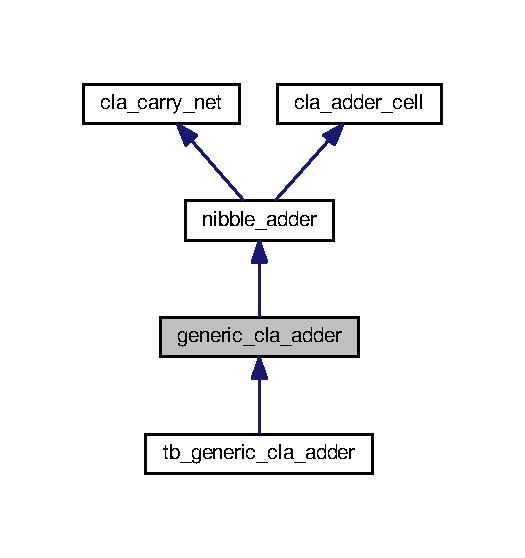
\includegraphics[width=319pt]{classgeneric__cla__adder__inherit__graph}
\end{center}
\end{figure}


Diagramma di collaborazione per generic\+\_\+cla\+\_\+adder\+:\nopagebreak
\begin{figure}[H]
\begin{center}
\leavevmode
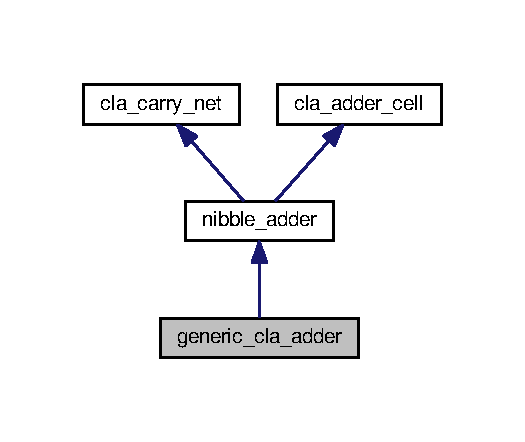
\includegraphics[width=252pt]{classgeneric__cla__adder__coll__graph}
\end{center}
\end{figure}
\subsection*{Entities}
\begin{DoxyCompactItemize}
\item 
\hyperlink{classgeneric__cla__adder_1_1structural}{structural} architecture
\begin{DoxyCompactList}\small\item\em Implementazione structural di \hyperlink{classgeneric__cla__adder}{generic\+\_\+cla\+\_\+adder}.

Questa implementazione istanzia tanti blocchi \hyperlink{classnibble__adder}{nibble\+\_\+adder} quanti siano i nibble in cui sono rappresentati gli addendi. La somma è espressa sullo stesso numero di bit. I diversi blocchi sono connessi tra loro come indicato nello schema ricordato di seguito\+: . \end{DoxyCompactList}\end{DoxyCompactItemize}
\subsection*{Generics}
 \begin{DoxyCompactItemize}
\item 
\hyperlink{group___carry_loockahead_ga0b63b586531492d0fa882246cca071c1}{nibbles} {\bfseries {\bfseries \textcolor{vhdlchar}{natural}\textcolor{vhdlchar}{ }\textcolor{vhdlchar}{ }\textcolor{vhdlchar}{\+:}\textcolor{vhdlchar}{=}\textcolor{vhdlchar}{ }\textcolor{vhdlchar}{ } \textcolor{vhdldigit}{2} \textcolor{vhdlchar}{ }}}
\end{DoxyCompactItemize}
\subsection*{Ports}
 \begin{DoxyCompactItemize}
\item 
\hyperlink{group___carry_loockahead_ga1c211cdf2d4cf97e869c442832c53439}{carry\+\_\+in}  {\bfseries {\bfseries \textcolor{vhdlchar}{in}\textcolor{vhdlchar}{ }}} {\bfseries \textcolor{vhdlchar}{std\+\_\+logic}\textcolor{vhdlchar}{ }} 
\item 
\hyperlink{group___carry_loockahead_gae4a2e124144a2f35270a55f0cf32a5ee}{addendum1}  {\bfseries {\bfseries \textcolor{vhdlchar}{in}\textcolor{vhdlchar}{ }}} {\bfseries \textcolor{vhdlchar}{std\+\_\+logic\+\_\+vector}\textcolor{vhdlchar}{ }\textcolor{vhdlchar}{(}\textcolor{vhdlchar}{ }\textcolor{vhdlchar}{(}\textcolor{vhdlchar}{ }\textcolor{vhdlchar}{ }\textcolor{vhdlchar}{ }\textcolor{vhdlchar}{ }{\bfseries \hyperlink{group___carry_loockahead_ga0b63b586531492d0fa882246cca071c1}{nibbles}} \textcolor{vhdlchar}{$\ast$}\textcolor{vhdlchar}{ } \textcolor{vhdldigit}{4} \textcolor{vhdlchar}{ }\textcolor{vhdlchar}{)}\textcolor{vhdlchar}{ }\textcolor{vhdlchar}{-\/}\textcolor{vhdlchar}{ } \textcolor{vhdldigit}{1} \textcolor{vhdlchar}{ }\textcolor{vhdlchar}{downto}\textcolor{vhdlchar}{ }\textcolor{vhdlchar}{ } \textcolor{vhdldigit}{0} \textcolor{vhdlchar}{ }\textcolor{vhdlchar}{)}\textcolor{vhdlchar}{ }} 
\begin{DoxyCompactList}\small\item\em addendo 1, espresso in complemento a due \end{DoxyCompactList}\item 
\hyperlink{group___carry_loockahead_ga2715463c615cf8418f85c6a1427ce62c}{addendum2}  {\bfseries {\bfseries \textcolor{vhdlchar}{in}\textcolor{vhdlchar}{ }}} {\bfseries \textcolor{vhdlchar}{std\+\_\+logic\+\_\+vector}\textcolor{vhdlchar}{ }\textcolor{vhdlchar}{(}\textcolor{vhdlchar}{ }\textcolor{vhdlchar}{(}\textcolor{vhdlchar}{ }\textcolor{vhdlchar}{ }\textcolor{vhdlchar}{ }\textcolor{vhdlchar}{ }{\bfseries \hyperlink{group___carry_loockahead_ga0b63b586531492d0fa882246cca071c1}{nibbles}} \textcolor{vhdlchar}{$\ast$}\textcolor{vhdlchar}{ } \textcolor{vhdldigit}{4} \textcolor{vhdlchar}{ }\textcolor{vhdlchar}{)}\textcolor{vhdlchar}{ }\textcolor{vhdlchar}{-\/}\textcolor{vhdlchar}{ } \textcolor{vhdldigit}{1} \textcolor{vhdlchar}{ }\textcolor{vhdlchar}{downto}\textcolor{vhdlchar}{ }\textcolor{vhdlchar}{ } \textcolor{vhdldigit}{0} \textcolor{vhdlchar}{ }\textcolor{vhdlchar}{)}\textcolor{vhdlchar}{ }} 
\begin{DoxyCompactList}\small\item\em addendo 2, espresso in complemento a due \end{DoxyCompactList}\item 
\hyperlink{group___carry_loockahead_ga1b4798a9e96bb32e9c08ce68e24e7871}{sum}  {\bfseries {\bfseries \textcolor{vhdlchar}{out}\textcolor{vhdlchar}{ }}} {\bfseries \textcolor{vhdlchar}{std\+\_\+logic\+\_\+vector}\textcolor{vhdlchar}{ }\textcolor{vhdlchar}{(}\textcolor{vhdlchar}{ }\textcolor{vhdlchar}{(}\textcolor{vhdlchar}{ }\textcolor{vhdlchar}{ }\textcolor{vhdlchar}{ }\textcolor{vhdlchar}{ }{\bfseries \hyperlink{group___carry_loockahead_ga0b63b586531492d0fa882246cca071c1}{nibbles}} \textcolor{vhdlchar}{$\ast$}\textcolor{vhdlchar}{ } \textcolor{vhdldigit}{4} \textcolor{vhdlchar}{ }\textcolor{vhdlchar}{)}\textcolor{vhdlchar}{ }\textcolor{vhdlchar}{-\/}\textcolor{vhdlchar}{ } \textcolor{vhdldigit}{1} \textcolor{vhdlchar}{ }\textcolor{vhdlchar}{downto}\textcolor{vhdlchar}{ }\textcolor{vhdlchar}{ } \textcolor{vhdldigit}{0} \textcolor{vhdlchar}{ }\textcolor{vhdlchar}{)}\textcolor{vhdlchar}{ }} 
\begin{DoxyCompactList}\small\item\em somma degli addendi, espressa in complemento a due \end{DoxyCompactList}\item 
\hyperlink{group___carry_loockahead_ga851aaea297bdc862fba5478c4bf0e214}{carry\+\_\+out}  {\bfseries {\bfseries \textcolor{vhdlchar}{out}\textcolor{vhdlchar}{ }}} {\bfseries \textcolor{vhdlchar}{std\+\_\+logic}\textcolor{vhdlchar}{ }} 
\item 
\hyperlink{group___carry_loockahead_ga9650307dde287e0bcfa1e26370c006c2}{overflow}  {\bfseries {\bfseries \textcolor{vhdlchar}{out}\textcolor{vhdlchar}{ }}} {\bfseries \textcolor{vhdlchar}{std\+\_\+logic}\textcolor{vhdlchar}{ }} 
\end{DoxyCompactItemize}


\subsection{Descrizione dettagliata}
Adder custom con carry-\/lookahead

\hyperlink{classgeneric__cla__adder}{generic\+\_\+cla\+\_\+adder} somma tra loro due addendi ed un carry in ingresso; gli addendi sono espressi su multipli interi di quattro bit. Oltre a generare la somma, genera il flag di carry ed il flag di overflow. 

La documentazione per questa classe è stata generata a partire dal seguente file\+:\begin{DoxyCompactItemize}
\item 
Src/adder/\hyperlink{generic__cla__adder_8vhd}{generic\+\_\+cla\+\_\+adder.\+vhd}\end{DoxyCompactItemize}

\hypertarget{class_linear_regression}{}\section{Linear\+Regression Entity Reference}
\label{class_linear_regression}\index{Linear\+Regression@{Linear\+Regression}}


Diagramma delle classi per Linear\+Regression\nopagebreak
\begin{figure}[H]
\begin{center}
\leavevmode
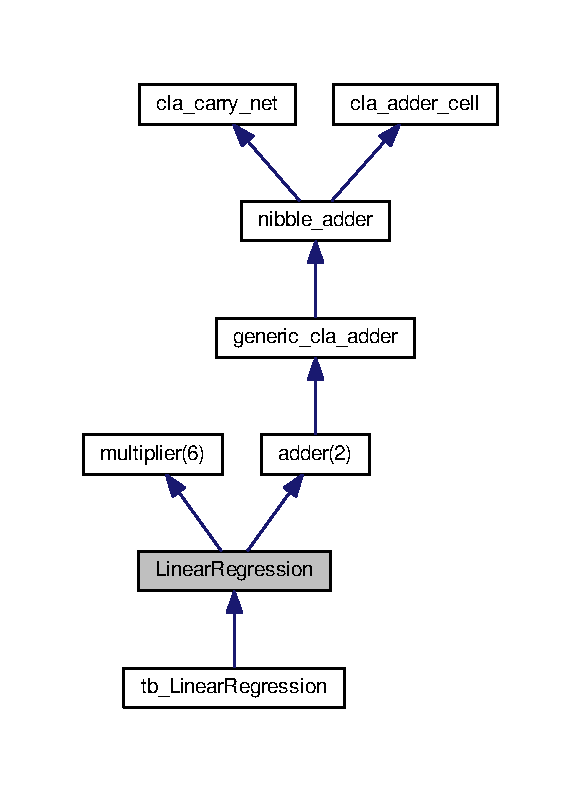
\includegraphics[width=279pt]{class_linear_regression__inherit__graph}
\end{center}
\end{figure}


Diagramma di collaborazione per Linear\+Regression\+:\nopagebreak
\begin{figure}[H]
\begin{center}
\leavevmode
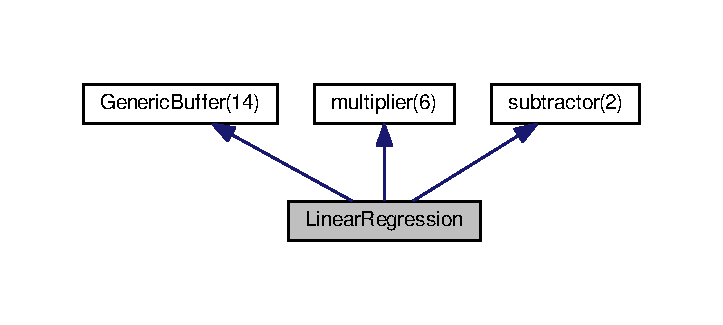
\includegraphics[width=279pt]{class_linear_regression__coll__graph}
\end{center}
\end{figure}
\subsection*{Entities}
\begin{DoxyCompactItemize}
\item 
\hyperlink{class_linear_regression_1_1_structural}{Structural} architecture
\end{DoxyCompactItemize}
\subsection*{Libraries}
 \begin{DoxyCompactItemize}
\item 
\hyperlink{group___linear_regression_gae4f03c286607f3181e16b9aa12d0c6d4}{I\+E\+EE} 
\end{DoxyCompactItemize}
\subsection*{Use Clauses}
 \begin{DoxyCompactItemize}
\item 
\hyperlink{group___linear_regression_gaa4b2b25246a821511120e3149b003563}{S\+T\+D\+\_\+\+L\+O\+G\+I\+C\+\_\+1164}   
\item 
\hyperlink{group___linear_regression_gae00f3f04545af57582ff10609eee23e2}{N\+U\+M\+E\+R\+I\+C\+\_\+\+S\+TD}   
\end{DoxyCompactItemize}
\subsection*{Ports}
 \begin{DoxyCompactItemize}
\item 
\hyperlink{group___linear_regression_ga6b9afe9c48db695b7336519281c099a8}{prim}  {\bfseries {\bfseries \textcolor{vhdlchar}{in}\textcolor{vhdlchar}{ }}} {\bfseries \textcolor{vhdlchar}{S\+T\+D\+\_\+\+L\+O\+G\+I\+C\+\_\+\+V\+E\+C\+T\+OR}\textcolor{vhdlchar}{ }\textcolor{vhdlchar}{(}\textcolor{vhdlchar}{ }\textcolor{vhdlchar}{ } \textcolor{vhdldigit}{4} \textcolor{vhdlchar}{ }\textcolor{vhdlchar}{downto}\textcolor{vhdlchar}{ }\textcolor{vhdlchar}{ } \textcolor{vhdldigit}{0} \textcolor{vhdlchar}{ }\textcolor{vhdlchar}{)}\textcolor{vhdlchar}{ }} 
\begin{DoxyCompactList}\small\item\em costante in input, 5 bit di parte intera e 0 decimale (m.\+n = 4.\+0) \end{DoxyCompactList}\item 
\hyperlink{group___linear_regression_ga4c98819455589b84c5e250a97e9bdfa1}{Sum2}  {\bfseries {\bfseries \textcolor{vhdlchar}{in}\textcolor{vhdlchar}{ }}} {\bfseries \textcolor{vhdlchar}{S\+T\+D\+\_\+\+L\+O\+G\+I\+C\+\_\+\+V\+E\+C\+T\+OR}\textcolor{vhdlchar}{ }\textcolor{vhdlchar}{(}\textcolor{vhdlchar}{ }\textcolor{vhdlchar}{ } \textcolor{vhdldigit}{23} \textcolor{vhdlchar}{ }\textcolor{vhdlchar}{downto}\textcolor{vhdlchar}{ }\textcolor{vhdlchar}{ } \textcolor{vhdldigit}{0} \textcolor{vhdlchar}{ }\textcolor{vhdlchar}{)}\textcolor{vhdlchar}{ }} 
\begin{DoxyCompactList}\small\item\em segnale in input, 3 bit di parte intera e 21 decimale (m.\+n = 2.\+21) \end{DoxyCompactList}\item 
\hyperlink{group___linear_regression_gab6685be06ffd9f2425d01307287a4454}{B}  {\bfseries {\bfseries \textcolor{vhdlchar}{in}\textcolor{vhdlchar}{ }}} {\bfseries \textcolor{vhdlchar}{S\+T\+D\+\_\+\+L\+O\+G\+I\+C\+\_\+\+V\+E\+C\+T\+OR}\textcolor{vhdlchar}{ }\textcolor{vhdlchar}{(}\textcolor{vhdlchar}{ }\textcolor{vhdlchar}{ } \textcolor{vhdldigit}{23} \textcolor{vhdlchar}{ }\textcolor{vhdlchar}{downto}\textcolor{vhdlchar}{ }\textcolor{vhdlchar}{ } \textcolor{vhdldigit}{0} \textcolor{vhdlchar}{ }\textcolor{vhdlchar}{)}\textcolor{vhdlchar}{ }} 
\begin{DoxyCompactList}\small\item\em segnale in input, 3 bit di parte intera e 21 decimale (m.\+n = 2.\+21) \end{DoxyCompactList}\item 
\hyperlink{group___linear_regression_ga43a9a0da4f44006af5631ed5ee8ad924}{Sum1}  {\bfseries {\bfseries \textcolor{vhdlchar}{in}\textcolor{vhdlchar}{ }}} {\bfseries \textcolor{vhdlchar}{S\+T\+D\+\_\+\+L\+O\+G\+I\+C\+\_\+\+V\+E\+C\+T\+OR}\textcolor{vhdlchar}{ }\textcolor{vhdlchar}{(}\textcolor{vhdlchar}{ }\textcolor{vhdlchar}{ } \textcolor{vhdldigit}{23} \textcolor{vhdlchar}{ }\textcolor{vhdlchar}{downto}\textcolor{vhdlchar}{ }\textcolor{vhdlchar}{ } \textcolor{vhdldigit}{0} \textcolor{vhdlchar}{ }\textcolor{vhdlchar}{)}\textcolor{vhdlchar}{ }} 
\begin{DoxyCompactList}\small\item\em segnale in input, 8 bit di parte intera e 16 decimale (m.\+n = 7.\+16) \end{DoxyCompactList}\item 
\hyperlink{group___linear_regression_ga17058a6bcb609074c49be51d09202870}{C}  {\bfseries {\bfseries \textcolor{vhdlchar}{in}\textcolor{vhdlchar}{ }}} {\bfseries \textcolor{vhdlchar}{S\+T\+D\+\_\+\+L\+O\+G\+I\+C\+\_\+\+V\+E\+C\+T\+OR}\textcolor{vhdlchar}{ }\textcolor{vhdlchar}{(}\textcolor{vhdlchar}{ }\textcolor{vhdlchar}{ } \textcolor{vhdldigit}{23} \textcolor{vhdlchar}{ }\textcolor{vhdlchar}{downto}\textcolor{vhdlchar}{ }\textcolor{vhdlchar}{ } \textcolor{vhdldigit}{0} \textcolor{vhdlchar}{ }\textcolor{vhdlchar}{)}\textcolor{vhdlchar}{ }} 
\begin{DoxyCompactList}\small\item\em segnale in input, msb di peso -\/10 (m.\+n = -\/10.\+33) \end{DoxyCompactList}\item 
\hyperlink{group___linear_regression_gae1ad6503d157f6c26abdce1131d31ec2}{A}  {\bfseries {\bfseries \textcolor{vhdlchar}{in}\textcolor{vhdlchar}{ }}} {\bfseries \textcolor{vhdlchar}{S\+T\+D\+\_\+\+L\+O\+G\+I\+C\+\_\+\+V\+E\+C\+T\+OR}\textcolor{vhdlchar}{ }\textcolor{vhdlchar}{(}\textcolor{vhdlchar}{ }\textcolor{vhdlchar}{ } \textcolor{vhdldigit}{23} \textcolor{vhdlchar}{ }\textcolor{vhdlchar}{downto}\textcolor{vhdlchar}{ }\textcolor{vhdlchar}{ } \textcolor{vhdldigit}{0} \textcolor{vhdlchar}{ }\textcolor{vhdlchar}{)}\textcolor{vhdlchar}{ }} 
\begin{DoxyCompactList}\small\item\em segnale in input, 16 bit di parte intera e 8 decimale (m.\+n = 15.\+8) \end{DoxyCompactList}\item 
\hyperlink{group___linear_regression_gad943f01112876248a4734aa3c3d2e3f2}{m}  {\bfseries {\bfseries \textcolor{vhdlchar}{out}\textcolor{vhdlchar}{ }}} {\bfseries \textcolor{vhdlchar}{S\+T\+D\+\_\+\+L\+O\+G\+I\+C\+\_\+\+V\+E\+C\+T\+OR}\textcolor{vhdlchar}{ }\textcolor{vhdlchar}{(}\textcolor{vhdlchar}{ }\textcolor{vhdlchar}{ } \textcolor{vhdldigit}{23} \textcolor{vhdlchar}{ }\textcolor{vhdlchar}{downto}\textcolor{vhdlchar}{ }\textcolor{vhdlchar}{ } \textcolor{vhdldigit}{0} \textcolor{vhdlchar}{ }\textcolor{vhdlchar}{)}\textcolor{vhdlchar}{ }} 
\begin{DoxyCompactList}\small\item\em segnale in output, 16 bit di parte intera e 8 decimale (m.\+n = 15.\+8) \end{DoxyCompactList}\item 
\hyperlink{group___linear_regression_gacec4f4b6d139d1ada088ca2d3d881418}{q}  {\bfseries {\bfseries \textcolor{vhdlchar}{out}\textcolor{vhdlchar}{ }}} {\bfseries \textcolor{vhdlchar}{S\+T\+D\+\_\+\+L\+O\+G\+I\+C\+\_\+\+V\+E\+C\+T\+OR}\textcolor{vhdlchar}{ }\textcolor{vhdlchar}{(}\textcolor{vhdlchar}{ }\textcolor{vhdlchar}{ } \textcolor{vhdldigit}{23} \textcolor{vhdlchar}{ }\textcolor{vhdlchar}{downto}\textcolor{vhdlchar}{ }\textcolor{vhdlchar}{ } \textcolor{vhdldigit}{0} \textcolor{vhdlchar}{ }\textcolor{vhdlchar}{)}\textcolor{vhdlchar}{ }} 
\begin{DoxyCompactList}\small\item\em segnaes in output, 8 bit di parte intera e 16 decimale (m.\+n = 7.\+16) \end{DoxyCompactList}\end{DoxyCompactItemize}


La documentazione per questa classe è stata generata a partire dal seguente file\+:\begin{DoxyCompactItemize}
\item 
Src/\hyperlink{_linear_regression_8vhd}{Linear\+Regression.\+vhd}\end{DoxyCompactItemize}

\hypertarget{classmultiplier}{}\section{multiplier Entity Reference}
\label{classmultiplier}\index{multiplier@{multiplier}}


Diagramma delle classi per multiplier\nopagebreak
\begin{figure}[H]
\begin{center}
\leavevmode
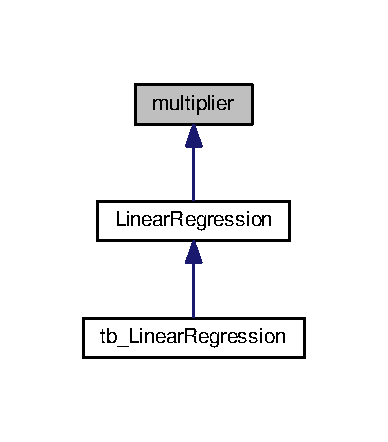
\includegraphics[width=278pt]{classmultiplier__inherit__graph}
\end{center}
\end{figure}
\subsection*{Entities}
\begin{DoxyCompactItemize}
\item 
\hyperlink{classmultiplier_1_1_structural}{Structural} architecture
\begin{DoxyCompactList}\small\item\em Per il prodotto viene utilizzato l\textquotesingle{}operatore $\ast$. La sintesi viene lasciata al particolare sintetizzatore. \end{DoxyCompactList}\end{DoxyCompactItemize}
\subsection*{Generics}
 \begin{DoxyCompactItemize}
\item 
\hyperlink{group___multiplier_ga4ede473cdc13e75fe66fbd548b62e432}{nbits1} {\bfseries {\bfseries \textcolor{vhdlchar}{natural}\textcolor{vhdlchar}{ }\textcolor{vhdlchar}{ }\textcolor{vhdlchar}{\+:}\textcolor{vhdlchar}{=}\textcolor{vhdlchar}{ }\textcolor{vhdlchar}{ } \textcolor{vhdldigit}{8} \textcolor{vhdlchar}{ }}}
\begin{DoxyCompactList}\small\item\em dimensione del primo fattore \end{DoxyCompactList}\item 
\hyperlink{group___multiplier_ga8b5bdaff4c3669528aaec95a07e17c2a}{nbits2} {\bfseries {\bfseries \textcolor{vhdlchar}{natural}\textcolor{vhdlchar}{ }\textcolor{vhdlchar}{ }\textcolor{vhdlchar}{\+:}\textcolor{vhdlchar}{=}\textcolor{vhdlchar}{ }\textcolor{vhdlchar}{ } \textcolor{vhdldigit}{8} \textcolor{vhdlchar}{ }}}
\begin{DoxyCompactList}\small\item\em dimensione del secondo fattore \end{DoxyCompactList}\end{DoxyCompactItemize}
\subsection*{Ports}
 \begin{DoxyCompactItemize}
\item 
\hyperlink{group___multiplier_gac728adecdbfe10213256c17c1b5c5128}{factor1}  {\bfseries {\bfseries \textcolor{vhdlchar}{in}\textcolor{vhdlchar}{ }}} {\bfseries \textcolor{vhdlchar}{S\+T\+D\+\_\+\+L\+O\+G\+I\+C\+\_\+\+V\+E\+C\+T\+OR}\textcolor{vhdlchar}{ }\textcolor{vhdlchar}{(}\textcolor{vhdlchar}{ }\textcolor{vhdlchar}{ }\textcolor{vhdlchar}{ }\textcolor{vhdlchar}{ }{\bfseries \hyperlink{group___multiplier_ga4ede473cdc13e75fe66fbd548b62e432}{nbits1}} \textcolor{vhdlchar}{-\/}\textcolor{vhdlchar}{ } \textcolor{vhdldigit}{1} \textcolor{vhdlchar}{ }\textcolor{vhdlchar}{downto}\textcolor{vhdlchar}{ }\textcolor{vhdlchar}{ } \textcolor{vhdldigit}{0} \textcolor{vhdlchar}{ }\textcolor{vhdlchar}{)}\textcolor{vhdlchar}{ }} 
\begin{DoxyCompactList}\small\item\em fattore 1 \end{DoxyCompactList}\item 
\hyperlink{group___multiplier_gac140852334303b430bbd49689cc689dd}{factor2}  {\bfseries {\bfseries \textcolor{vhdlchar}{in}\textcolor{vhdlchar}{ }}} {\bfseries \textcolor{vhdlchar}{S\+T\+D\+\_\+\+L\+O\+G\+I\+C\+\_\+\+V\+E\+C\+T\+OR}\textcolor{vhdlchar}{ }\textcolor{vhdlchar}{(}\textcolor{vhdlchar}{ }\textcolor{vhdlchar}{ }\textcolor{vhdlchar}{ }\textcolor{vhdlchar}{ }{\bfseries \hyperlink{group___multiplier_ga8b5bdaff4c3669528aaec95a07e17c2a}{nbits2}} \textcolor{vhdlchar}{-\/}\textcolor{vhdlchar}{ } \textcolor{vhdldigit}{1} \textcolor{vhdlchar}{ }\textcolor{vhdlchar}{downto}\textcolor{vhdlchar}{ }\textcolor{vhdlchar}{ } \textcolor{vhdldigit}{0} \textcolor{vhdlchar}{ }\textcolor{vhdlchar}{)}\textcolor{vhdlchar}{ }} 
\begin{DoxyCompactList}\small\item\em fattore 2 \end{DoxyCompactList}\item 
\hyperlink{group___multiplier_gaf168dc69ad77dc5791b5e0f99dcfb0a9}{prod}  {\bfseries {\bfseries \textcolor{vhdlchar}{out}\textcolor{vhdlchar}{ }}} {\bfseries \textcolor{vhdlchar}{S\+T\+D\+\_\+\+L\+O\+G\+I\+C\+\_\+\+V\+E\+C\+T\+OR}\textcolor{vhdlchar}{ }\textcolor{vhdlchar}{(}\textcolor{vhdlchar}{ }\textcolor{vhdlchar}{ }\textcolor{vhdlchar}{ }\textcolor{vhdlchar}{ }{\bfseries \hyperlink{group___multiplier_ga4ede473cdc13e75fe66fbd548b62e432}{nbits1}} \textcolor{vhdlchar}{+}\textcolor{vhdlchar}{ }\textcolor{vhdlchar}{ }\textcolor{vhdlchar}{ }{\bfseries \hyperlink{group___multiplier_ga8b5bdaff4c3669528aaec95a07e17c2a}{nbits2}} \textcolor{vhdlchar}{-\/}\textcolor{vhdlchar}{ } \textcolor{vhdldigit}{1} \textcolor{vhdlchar}{ }\textcolor{vhdlchar}{downto}\textcolor{vhdlchar}{ }\textcolor{vhdlchar}{ } \textcolor{vhdldigit}{0} \textcolor{vhdlchar}{ }\textcolor{vhdlchar}{)}\textcolor{vhdlchar}{ }} 
\begin{DoxyCompactList}\small\item\em prodotto dei due fattori \end{DoxyCompactList}\end{DoxyCompactItemize}


\subsection{Descrizione dettagliata}
Moltiplicatore a due fattori.

Il moltiplicatore permette di effettuare un prodotto di due fattori espressi su un certo numero di bit. I due fattori possono essere espressi anche su un numero di bit e rappresentazioni differenti tra loro. Se nbit1 è il numero di bit su cui viene espresso il fattore 1, e nbit2 è il numero di bit su cui viene espresso il fattore 2, allora l\textquotesingle{}uscita prod risulta essere espressa su nbit1+nbit2. ~\newline
 Ad esempio, se il fattore 1 è rappresentato con mx.\+nx (con mx il peso del bit più significativo della parte intera ed nx il peso del bit meno significativo della parte decimale) e il fattore 2 è rappresentato con my.\+ny, allora l\textquotesingle{}uscita sarà rappresentata in mx+my+1.nx+ny 

La documentazione per questa classe è stata generata a partire dal seguente file\+:\begin{DoxyCompactItemize}
\item 
Src/\hyperlink{multiplier_8vhd}{multiplier.\+vhd}\end{DoxyCompactItemize}

\hypertarget{classnibble__adder}{}\section{nibble\+\_\+adder Entity Reference}
\label{classnibble__adder}\index{nibble\+\_\+adder@{nibble\+\_\+adder}}


Addizionatore con carry-\/lookahead a quattro bit.

La cella somma tra loro due addendi ed un carry in ingresso; gli addendi sono espressi su quattro bit. Oltre a generare la somma, genera le funzioni \char`\"{}propagazione\char`\"{} e \char`\"{}generazione\char`\"{} del carry per eventuali blocchi \hyperlink{classnibble__adder}{nibble\+\_\+adder} posti a valle.  




Diagramma delle classi per nibble\+\_\+adder
\nopagebreak
\begin{figure}[H]
\begin{center}
\leavevmode
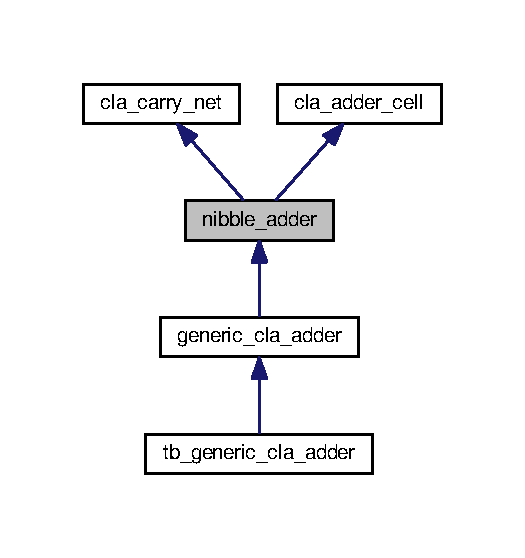
\includegraphics[width=319pt]{classnibble__adder__inherit__graph}
\end{center}
\end{figure}


Diagramma di collaborazione per nibble\+\_\+adder\+:
\nopagebreak
\begin{figure}[H]
\begin{center}
\leavevmode
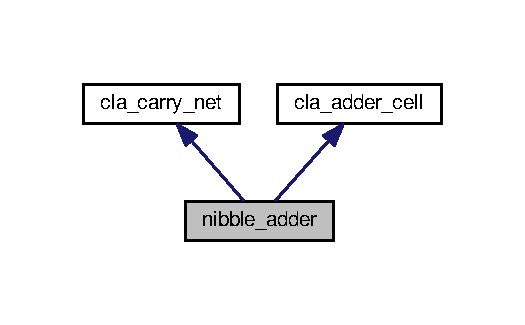
\includegraphics[width=252pt]{classnibble__adder__coll__graph}
\end{center}
\end{figure}
\subsection*{Entities}
\begin{DoxyCompactItemize}
\item 
\hyperlink{classnibble__adder_1_1structural}{structural} architecture
\begin{DoxyCompactList}\small\item\em Implementazione structural dell\textquotesingle{}entità \hyperlink{classnibble__adder}{nibble\+\_\+adder}.

Questa architettura istanzia una entità \hyperlink{classcla__carry__net}{cla\+\_\+carry\+\_\+net} ed una entità \hyperlink{classcla__adder__cell}{cla\+\_\+adder\+\_\+cell} per ogni bit su cui sono espressi gli addendi, connettendoli tra loro secondo lo schema riportato di seguito\+: . \end{DoxyCompactList}\end{DoxyCompactItemize}
\subsection*{Ports}
 \begin{DoxyCompactItemize}
\item 
\hyperlink{group___nibble_adder_ga2c8945f4747b9a5448412c95fc281c87}{addendum1}  {\bfseries {\bfseries \textcolor{vhdlchar}{in}\textcolor{vhdlchar}{ }}} {\bfseries \textcolor{vhdlchar}{std\+\_\+logic\+\_\+vector}\textcolor{vhdlchar}{ }\textcolor{vhdlchar}{(}\textcolor{vhdlchar}{ }\textcolor{vhdlchar}{ } \textcolor{vhdldigit}{3} \textcolor{vhdlchar}{ }\textcolor{vhdlchar}{downto}\textcolor{vhdlchar}{ }\textcolor{vhdlchar}{ } \textcolor{vhdldigit}{0} \textcolor{vhdlchar}{ }\textcolor{vhdlchar}{)}\textcolor{vhdlchar}{ }} 
\begin{DoxyCompactList}\small\item\em addendo 1 \end{DoxyCompactList}\item 
\hyperlink{group___nibble_adder_gad1fa6d9d78208885ad2f4c417fc4b530}{addendum2}  {\bfseries {\bfseries \textcolor{vhdlchar}{in}\textcolor{vhdlchar}{ }}} {\bfseries \textcolor{vhdlchar}{std\+\_\+logic\+\_\+vector}\textcolor{vhdlchar}{ }\textcolor{vhdlchar}{(}\textcolor{vhdlchar}{ }\textcolor{vhdlchar}{ } \textcolor{vhdldigit}{3} \textcolor{vhdlchar}{ }\textcolor{vhdlchar}{downto}\textcolor{vhdlchar}{ }\textcolor{vhdlchar}{ } \textcolor{vhdldigit}{0} \textcolor{vhdlchar}{ }\textcolor{vhdlchar}{)}\textcolor{vhdlchar}{ }} 
\begin{DoxyCompactList}\small\item\em addendo 2 \end{DoxyCompactList}\item 
\hyperlink{group___nibble_adder_gaa556a73dc4a4de1a0d662b25adbcbe33}{carryin}  {\bfseries {\bfseries \textcolor{vhdlchar}{in}\textcolor{vhdlchar}{ }}} {\bfseries \textcolor{vhdlchar}{std\+\_\+logic}\textcolor{vhdlchar}{ }} 
\begin{DoxyCompactList}\small\item\em segnale di \char`\"{}carry-\/in\char`\"{}, prodotto da un eventuale \hyperlink{classnibble__adder}{nibble\+\_\+adder} a monte. \end{DoxyCompactList}\item 
\hyperlink{group___nibble_adder_ga422e8e7ee01fc7ac7b7390cd2ad8c87b}{propin}  {\bfseries {\bfseries \textcolor{vhdlchar}{in}\textcolor{vhdlchar}{ }}} {\bfseries \textcolor{vhdlchar}{std\+\_\+logic}\textcolor{vhdlchar}{ }} 
\begin{DoxyCompactList}\small\item\em funzione \char`\"{}propagazione\char`\"{}, prodotta da una eventuale \hyperlink{classnibble__adder}{nibble\+\_\+adder} a monte \end{DoxyCompactList}\item 
\hyperlink{group___nibble_adder_ga0a46d5193cb73eb993bc5d4f69741d0a}{genin}  {\bfseries {\bfseries \textcolor{vhdlchar}{in}\textcolor{vhdlchar}{ }}} {\bfseries \textcolor{vhdlchar}{std\+\_\+logic}\textcolor{vhdlchar}{ }} 
\begin{DoxyCompactList}\small\item\em funzione \char`\"{}generazione\char`\"{}, prodotta da una eventuale \hyperlink{classnibble__adder}{nibble\+\_\+adder} a monte \end{DoxyCompactList}\item 
\hyperlink{group___nibble_adder_ga5957c9cdd706cafd2da8855133a002c9}{propout}  {\bfseries {\bfseries \textcolor{vhdlchar}{out}\textcolor{vhdlchar}{ }}} {\bfseries \textcolor{vhdlchar}{std\+\_\+logic}\textcolor{vhdlchar}{ }} 
\item 
\hyperlink{group___nibble_adder_ga068cd5c4d23e284cb942702252ed1491}{genout}  {\bfseries {\bfseries \textcolor{vhdlchar}{out}\textcolor{vhdlchar}{ }}} {\bfseries \textcolor{vhdlchar}{std\+\_\+logic}\textcolor{vhdlchar}{ }} 
\item 
\hyperlink{group___nibble_adder_gadfe538323c3296159dd3b383325a996b}{sum}  {\bfseries {\bfseries \textcolor{vhdlchar}{out}\textcolor{vhdlchar}{ }}} {\bfseries \textcolor{vhdlchar}{std\+\_\+logic\+\_\+vector}\textcolor{vhdlchar}{ }\textcolor{vhdlchar}{(}\textcolor{vhdlchar}{ }\textcolor{vhdlchar}{ } \textcolor{vhdldigit}{3} \textcolor{vhdlchar}{ }\textcolor{vhdlchar}{downto}\textcolor{vhdlchar}{ }\textcolor{vhdlchar}{ } \textcolor{vhdldigit}{0} \textcolor{vhdlchar}{ }\textcolor{vhdlchar}{)}\textcolor{vhdlchar}{ }} 
\end{DoxyCompactItemize}


\subsection{Descrizione dettagliata}
Addizionatore con carry-\/lookahead a quattro bit.

La cella somma tra loro due addendi ed un carry in ingresso; gli addendi sono espressi su quattro bit. Oltre a generare la somma, genera le funzioni \char`\"{}propagazione\char`\"{} e \char`\"{}generazione\char`\"{} del carry per eventuali blocchi \hyperlink{classnibble__adder}{nibble\+\_\+adder} posti a valle. 

La documentazione per questa classe è stata generata a partire dal seguente file\+:\begin{DoxyCompactItemize}
\item 
Src/adder/\hyperlink{nibble__adder_8vhd}{nibble\+\_\+adder.\+vhd}\end{DoxyCompactItemize}

\hypertarget{classmultiplier_1_1_structural}{}\section{Structural Architecture Reference}
\label{classmultiplier_1_1_structural}\index{Structural@{Structural}}


Per il prodotto viene utilizzato l\textquotesingle{}operatore $\ast$. La sintesi viene lasciata al particolare sintetizzatore.  




\subsection{Descrizione dettagliata}
Per il prodotto viene utilizzato l\textquotesingle{}operatore $\ast$. La sintesi viene lasciata al particolare sintetizzatore. 

La documentazione per questa classe è stata generata a partire dal seguente file\+:\begin{DoxyCompactItemize}
\item 
Src/\hyperlink{multiplier_8vhd}{multiplier.\+vhd}\end{DoxyCompactItemize}

\hypertarget{classadder_1_1structural}{}\section{structural Architecture Reference}
\label{classadder_1_1structural}\index{structural@{structural}}


Implementazione mista structural per l\textquotesingle{}entity adder.

A seconda del valore del parametro use\+\_\+custom, verrà istanziato
\begin{DoxyItemize}
\item un sommatore full-\/custom \hyperlink{classgeneric__cla__adder}{generic\+\_\+cla\+\_\+adder}, se use\+\_\+custom = true;
\item un sommatore la cui implementazione è stabilita dal sintetizzatore, se use\+\_\+custom = false; Nel caso in cui venga istanziato il sommatore custom, è richiesto che il numero di bit con il quale sono espressi gli addendi, e di conseguenza quello in vui verrà espressa la loro somma, sia multiplo di quattro. 
\end{DoxyItemize} 


\subsection*{Components}
 \begin{DoxyCompactItemize}
\item 
\hyperlink{group___adder_gae7148956d4ef1d1cd14f35060634b9c3}{generic\+\_\+cla\+\_\+adder}  {\bfseries }  
\end{DoxyCompactItemize}
\subsection*{Signals}
 \begin{DoxyCompactItemize}
\item 
\hyperlink{group___adder_ga590914af948ec283f1371002f2f76720}{sum\+\_\+tmp} {\bfseries \textcolor{vhdlchar}{std\+\_\+logic\+\_\+vector}\textcolor{vhdlchar}{ }\textcolor{vhdlchar}{(}\textcolor{vhdlchar}{ }\textcolor{vhdlchar}{ }\textcolor{vhdlchar}{ }\textcolor{vhdlchar}{ }{\bfseries \hyperlink{group___adder_gae1435c07d0cd54b521535e2f8de6f94e}{nbits}} \textcolor{vhdlchar}{-\/}\textcolor{vhdlchar}{ } \textcolor{vhdldigit}{1} \textcolor{vhdlchar}{ }\textcolor{vhdlchar}{downto}\textcolor{vhdlchar}{ }\textcolor{vhdlchar}{ } \textcolor{vhdldigit}{0} \textcolor{vhdlchar}{ }\textcolor{vhdlchar}{)}\textcolor{vhdlchar}{ }} 
\end{DoxyCompactItemize}
\subsection*{Instantiations}
 \begin{DoxyCompactItemize}
\item 
\hyperlink{classadder_1_1structural_a94015e32a32cd4c5be09b1ddde822259}{cla\+\_\+adder}  {\bfseries generic\+\_\+cla\+\_\+adder}   
\end{DoxyCompactItemize}


\subsection{Descrizione dettagliata}
Implementazione mista structural per l\textquotesingle{}entity adder.

A seconda del valore del parametro use\+\_\+custom, verrà istanziato
\begin{DoxyItemize}
\item un sommatore full-\/custom \hyperlink{classgeneric__cla__adder}{generic\+\_\+cla\+\_\+adder}, se use\+\_\+custom = true;
\item un sommatore la cui implementazione è stabilita dal sintetizzatore, se use\+\_\+custom = false; Nel caso in cui venga istanziato il sommatore custom, è richiesto che il numero di bit con il quale sono espressi gli addendi, e di conseguenza quello in vui verrà espressa la loro somma, sia multiplo di quattro. 
\end{DoxyItemize}

flag di overflow; è \textquotesingle{}1\textquotesingle{} quando il risultato prodotto dalla somma degli addendi non è rappresentabile su 4$\ast$nibbles bit\+: si verifica overflow se, sommando due numeri dello stesso segno, si ottiene un numero di segno opposto. 

\subsection{Documentazione dei membri dato}
\mbox{\Hypertarget{classadder_1_1structural_a94015e32a32cd4c5be09b1ddde822259}\label{classadder_1_1structural_a94015e32a32cd4c5be09b1ddde822259}} 
\index{adder\+::structural@{adder\+::structural}!cla\+\_\+adder@{cla\+\_\+adder}}
\index{cla\+\_\+adder@{cla\+\_\+adder}!adder\+::structural@{adder\+::structural}}
\subsubsection{\texorpdfstring{cla\+\_\+adder}{cla\_adder}}
{\footnotesize\ttfamily \hyperlink{classadder_1_1structural_a94015e32a32cd4c5be09b1ddde822259}{cla\+\_\+adder} {\bfseries \textcolor{vhdlchar}{generic\+\_\+cla\+\_\+adder}\textcolor{vhdlchar}{ }} \hspace{0.3cm}{\ttfamily [Instantiation]}}

segnale temporaneo nel quale viene posto il risultato della somma per effettuare il calcolo della condizione di overflow 

La documentazione per questa classe è stata generata a partire dal seguente file\+:\begin{DoxyCompactItemize}
\item 
Src/adder/\hyperlink{adder_8vhd}{adder.\+vhd}\end{DoxyCompactItemize}

\hypertarget{classnibble__adder_1_1structural}{\section{structural Architecture Reference}
\label{classnibble__adder_1_1structural}\index{structural@{structural}}
}


Implementazione structural dell'entità \hyperlink{classnibble__adder}{nibble\+\_\+adder}.  


\subsection*{Components}
 \begin{DoxyCompactItemize}
\item 
\hyperlink{group___nibble_adder_ga12bdc5892f526938e1447d663d152df8}{cla\+\_\+carry\+\_\+net}  {\bfseries }  
\item 
\hyperlink{group___nibble_adder_ga4f13eb52457f650b1d2cd352d9cacca9}{cla\+\_\+adder\+\_\+cell}  {\bfseries }  
\end{DoxyCompactItemize}
\subsection*{Instantiations}
 \begin{DoxyCompactItemize}
\item 
\hyperlink{classnibble__adder_1_1structural_abbf8fdf15c2d70392ab929c8ebe57439}{cla\+\_\+net}  {\bfseries cla\+\_\+carry\+\_\+net}   
\begin{DoxyCompactList}\small\item\em funzione “propagazione” prodotta da \hyperlink{classcla__adder__cell}{cla\+\_\+adder\+\_\+cell}; vale 1 quando, sulla base degli ingressi, un adder propaghera' un eventuale carry in ingresso; prop(i) = add(i) O\+R add(i); in questo caso viene prodotta da quattro blocchi \hyperlink{classcla__adder__cell}{cla\+\_\+adder\+\_\+cell} sulla base dei loro ingressi \end{DoxyCompactList}\item 
\hyperlink{classnibble__adder_1_1structural_a9d7a8a381439c61aea549e7a47ec7a6f}{adder}  {\bfseries cla\+\_\+adder\+\_\+cell}   
\end{DoxyCompactItemize}


\subsection{Descrizione dettagliata}
Implementazione structural dell'entità \hyperlink{classnibble__adder}{nibble\+\_\+adder}. 

Questa architettura istanzia una entità \hyperlink{classcla__carry__net}{cla\+\_\+carry\+\_\+net} ed una entità \hyperlink{classcla__adder__cell}{cla\+\_\+adder\+\_\+cell} per ogni bit su cui sono espressi gli addendi, connettendoli tra loro secondo lo schema riportato di seguito\+:  

\subsection{Documentazione dei membri dato}
\hypertarget{classnibble__adder_1_1structural_a9d7a8a381439c61aea549e7a47ec7a6f}{\index{nibble\+\_\+adder\+::structural@{nibble\+\_\+adder\+::structural}!adder@{adder}}
\index{adder@{adder}!nibble\+\_\+adder\+::structural@{nibble\+\_\+adder\+::structural}}
\subsubsection[{adder}]{\setlength{\rightskip}{0pt plus 5cm}{\bf adder} {\bfseries \textcolor{vhdlchar}{cla\+\_\+adder\+\_\+cell}\textcolor{vhdlchar}{ }} \hspace{0.3cm}{\ttfamily [Instantiation]}}}\label{classnibble__adder_1_1structural_a9d7a8a381439c61aea549e7a47ec7a6f}
\hypertarget{classnibble__adder_1_1structural_abbf8fdf15c2d70392ab929c8ebe57439}{\index{nibble\+\_\+adder\+::structural@{nibble\+\_\+adder\+::structural}!cla\+\_\+net@{cla\+\_\+net}}
\index{cla\+\_\+net@{cla\+\_\+net}!nibble\+\_\+adder\+::structural@{nibble\+\_\+adder\+::structural}}
\subsubsection[{cla\+\_\+net}]{\setlength{\rightskip}{0pt plus 5cm}{\bf cla\+\_\+net} {\bfseries \textcolor{vhdlchar}{cla\+\_\+carry\+\_\+net}\textcolor{vhdlchar}{ }} \hspace{0.3cm}{\ttfamily [Instantiation]}}}\label{classnibble__adder_1_1structural_abbf8fdf15c2d70392ab929c8ebe57439}


funzione “propagazione” prodotta da \hyperlink{classcla__adder__cell}{cla\+\_\+adder\+\_\+cell}; vale 1 quando, sulla base degli ingressi, un adder propaghera' un eventuale carry in ingresso; prop(i) = add(i) O\+R add(i); in questo caso viene prodotta da quattro blocchi \hyperlink{classcla__adder__cell}{cla\+\_\+adder\+\_\+cell} sulla base dei loro ingressi 

carry calcolati sulla base delle funzioni \char`\"{}propagazione\char`\"{} e \char`\"{}generazione\char`\"{} prodotti dai blocchi \hyperlink{classcla__adder__cell}{cla\+\_\+adder\+\_\+cell}, e sulla base delle funzioni \char`\"{}carry-\/in\char`\"{}, \char`\"{}propagazione\char`\"{} e \char`\"{}generazione\char`\"{} prodotti da eventuali blocchi a monte; ciascuno dei bit dovra' essere posto in ingresso ad un blocco \hyperlink{classcla__adder__cell}{cla\+\_\+adder\+\_\+cell} differente, affinche' possa essere calcolata la somma degli addendi 

La documentazione per questa classe è stata generata a partire dal seguente file\+:\begin{DoxyCompactItemize}
\item 
Src/adder/\hyperlink{nibble__adder_8vhd}{nibble\+\_\+adder.\+vhd}\end{DoxyCompactItemize}

\hypertarget{class_linear_regression_1_1_structural}{}\section{Structural Architecture Reference}
\label{class_linear_regression_1_1_structural}\index{Structural@{Structural}}


8 

M\+U\+L\+T1, M\+U\+L\+T2, M\+U\+L\+T3, M\+U\+L\+T4, A\+D\+D5, A\+D\+D6, M\+U\+L\+T6 

Verificare che il troncamento post M\+U\+L\+T6 venga effettuato correttamente (7 bit in testa e 17 in coda) 

C=b\char`\"{}011000011101000101011010\char`\"{}~\newline
 Sum2=b\char`\"{}001010111100110111101111\char`\"{}~\newline
 B=b\char`\"{}001000110100010101100111\char`\"{}~\newline
 Sum1=b\char`\"{}001101001011110110010011\char`\"{}~\newline
 A=b\char`\"{}000111101111000111001010\char`\"{}  

mult2\+\_\+out=b\char`\"{}000001100000100100000111110011100100011000101001\char`\"{}~\newline
 P2= b\char`\"{}000010010000011111001110\char`\"{}~\newline
 mult4\+\_\+out=b\char`\"{}000101000010011011110110000000101010100010101110\char`\"{}~\newline
 P4= b\char`\"{}001010000100110111101100\char`\"{}~\newline
 add2\+\_\+out= b\char`\"{}001100010101010110111010\char`\"{}~\newline
 S6= b\char`\"{}000110001010101011011101\char`\"{}~\newline
 mult1\+\_\+out=b\char`\"{}00001101101100000101101010110\char`\"{}~\newline
 P3= b\char`\"{}011011011000001011010101\char`\"{}~\newline
 mult3\+\_\+out=b\char`\"{}000001110100010000110111011010011110010100100101\char`\"{}~\newline
 P1= b\char`\"{}110100010000110111011010\char`\"{}~\newline
 S5= b\char`\"{}001111101001000010101111\char`\"{}~\newline
 mult6\+\_\+out=b\char`\"{}000000101111101101010010001101101101111101100010\char`\"{}~\newline
 q =b\char`\"{}011111011010100100011011\char`\"{}  

mult2\+\_\+out=b\char`\"{}000001100000100100000111110011100100011000101001\char`\"{}~\newline
 P2= b\char`\"{}000010010000011111001110\char`\"{}~\newline
 mult4\+\_\+out=b\char`\"{}000101000010011011110110000000101010100010101110\char`\"{}~\newline
 P4= b\char`\"{}001010000100110111101100\char`\"{}~\newline
 add2\+\_\+out= b\char`\"{}001100010101010110111010\char`\"{}~\newline
 S6= b\char`\"{}000110001010101011011101\char`\"{}~\newline
 mult1\+\_\+out=b\char`\"{}00001101101100000101101010110\char`\"{}~\newline
 P3= b\char`\"{}011011011000001011010101\char`\"{}~\newline
 mult3\+\_\+out=b\char`\"{}000001110100010000110111011010011110010100100101\char`\"{}~\newline
 P1= b\char`\"{}110100010000110111011010\char`\"{}~\newline
 S5= b\char`\"{}001111101001000010101111\char`\"{}~\newline
 mult6\+\_\+out=b\char`\"{}000000101111101101010010001101101101111101100010\char`\"{}~\newline
 q =b\char`\"{}       011111011010100100011011\char`\"{}  

Superato   


\subsection*{Components}
 \begin{DoxyCompactItemize}
\item 
\hyperlink{group___linear_regression_ga3cf9cbfc3e637ae0660c32ceef50386f}{multiplier}  {\bfseries }  
\item 
\hyperlink{group___linear_regression_ga9d7a8a381439c61aea549e7a47ec7a6f}{adder}  {\bfseries }  
\end{DoxyCompactItemize}
\subsection*{Signals}
 \begin{DoxyCompactItemize}
\item 
\hyperlink{group___linear_regression_ga8e3ef6c468a1560f19de3430d956a75c}{mult1\+\_\+out} {\bfseries \textcolor{vhdlchar}{std\+\_\+logic\+\_\+vector}\textcolor{vhdlchar}{ }\textcolor{vhdlchar}{(}\textcolor{vhdlchar}{ }\textcolor{vhdlchar}{ } \textcolor{vhdldigit}{28} \textcolor{vhdlchar}{ }\textcolor{vhdlchar}{downto}\textcolor{vhdlchar}{ }\textcolor{vhdlchar}{ } \textcolor{vhdldigit}{0} \textcolor{vhdlchar}{ }\textcolor{vhdlchar}{)}\textcolor{vhdlchar}{ }\textcolor{vhdlchar}{ }\textcolor{vhdlchar}{ }\textcolor{vhdlchar}{\+:}\textcolor{vhdlchar}{=}\textcolor{vhdlchar}{ }\textcolor{vhdlchar}{(}\textcolor{vhdlchar}{ }\textcolor{vhdlchar}{ }\textcolor{vhdlchar}{others}\textcolor{vhdlchar}{ }\textcolor{vhdlchar}{ }\textcolor{vhdlchar}{=}\textcolor{vhdlchar}{ }\textcolor{vhdlchar}{$>$}\textcolor{vhdlchar}{ }\textcolor{vhdlchar}{\textquotesingle{}}\textcolor{vhdlchar}{ } \textcolor{vhdldigit}{0} \textcolor{vhdlchar}{ }\textcolor{vhdlchar}{\textquotesingle{}}\textcolor{vhdlchar}{ }\textcolor{vhdlchar}{)}\textcolor{vhdlchar}{ }} 
\item 
\hyperlink{group___linear_regression_gaa427886ed37e5d29753362483ce7fae2}{P3} {\bfseries \textcolor{vhdlchar}{std\+\_\+logic\+\_\+vector}\textcolor{vhdlchar}{ }\textcolor{vhdlchar}{(}\textcolor{vhdlchar}{ }\textcolor{vhdlchar}{ } \textcolor{vhdldigit}{23} \textcolor{vhdlchar}{ }\textcolor{vhdlchar}{downto}\textcolor{vhdlchar}{ }\textcolor{vhdlchar}{ } \textcolor{vhdldigit}{0} \textcolor{vhdlchar}{ }\textcolor{vhdlchar}{)}\textcolor{vhdlchar}{ }\textcolor{vhdlchar}{ }\textcolor{vhdlchar}{ }\textcolor{vhdlchar}{\+:}\textcolor{vhdlchar}{=}\textcolor{vhdlchar}{ }\textcolor{vhdlchar}{(}\textcolor{vhdlchar}{ }\textcolor{vhdlchar}{ }\textcolor{vhdlchar}{others}\textcolor{vhdlchar}{ }\textcolor{vhdlchar}{ }\textcolor{vhdlchar}{=}\textcolor{vhdlchar}{ }\textcolor{vhdlchar}{$>$}\textcolor{vhdlchar}{ }\textcolor{vhdlchar}{\textquotesingle{}}\textcolor{vhdlchar}{ } \textcolor{vhdldigit}{0} \textcolor{vhdlchar}{ }\textcolor{vhdlchar}{\textquotesingle{}}\textcolor{vhdlchar}{ }\textcolor{vhdlchar}{)}\textcolor{vhdlchar}{ }} 
\item 
\hyperlink{group___linear_regression_gac6c586bcd10a70e181cf575558678c99}{mult2\+\_\+out} {\bfseries \textcolor{vhdlchar}{std\+\_\+logic\+\_\+vector}\textcolor{vhdlchar}{ }\textcolor{vhdlchar}{(}\textcolor{vhdlchar}{ }\textcolor{vhdlchar}{ } \textcolor{vhdldigit}{47} \textcolor{vhdlchar}{ }\textcolor{vhdlchar}{downto}\textcolor{vhdlchar}{ }\textcolor{vhdlchar}{ } \textcolor{vhdldigit}{0} \textcolor{vhdlchar}{ }\textcolor{vhdlchar}{)}\textcolor{vhdlchar}{ }\textcolor{vhdlchar}{ }\textcolor{vhdlchar}{ }\textcolor{vhdlchar}{\+:}\textcolor{vhdlchar}{=}\textcolor{vhdlchar}{ }\textcolor{vhdlchar}{(}\textcolor{vhdlchar}{ }\textcolor{vhdlchar}{ }\textcolor{vhdlchar}{others}\textcolor{vhdlchar}{ }\textcolor{vhdlchar}{ }\textcolor{vhdlchar}{=}\textcolor{vhdlchar}{ }\textcolor{vhdlchar}{$>$}\textcolor{vhdlchar}{ }\textcolor{vhdlchar}{\textquotesingle{}}\textcolor{vhdlchar}{ } \textcolor{vhdldigit}{0} \textcolor{vhdlchar}{ }\textcolor{vhdlchar}{\textquotesingle{}}\textcolor{vhdlchar}{ }\textcolor{vhdlchar}{)}\textcolor{vhdlchar}{ }} 
\item 
\hyperlink{group___linear_regression_gab0bf0189296a8c52f6e36c853c8d3a77}{P2} {\bfseries \textcolor{vhdlchar}{std\+\_\+logic\+\_\+vector}\textcolor{vhdlchar}{ }\textcolor{vhdlchar}{(}\textcolor{vhdlchar}{ }\textcolor{vhdlchar}{ } \textcolor{vhdldigit}{23} \textcolor{vhdlchar}{ }\textcolor{vhdlchar}{downto}\textcolor{vhdlchar}{ }\textcolor{vhdlchar}{ } \textcolor{vhdldigit}{0} \textcolor{vhdlchar}{ }\textcolor{vhdlchar}{)}\textcolor{vhdlchar}{ }\textcolor{vhdlchar}{ }\textcolor{vhdlchar}{ }\textcolor{vhdlchar}{\+:}\textcolor{vhdlchar}{=}\textcolor{vhdlchar}{ }\textcolor{vhdlchar}{(}\textcolor{vhdlchar}{ }\textcolor{vhdlchar}{ }\textcolor{vhdlchar}{others}\textcolor{vhdlchar}{ }\textcolor{vhdlchar}{ }\textcolor{vhdlchar}{=}\textcolor{vhdlchar}{ }\textcolor{vhdlchar}{$>$}\textcolor{vhdlchar}{ }\textcolor{vhdlchar}{\textquotesingle{}}\textcolor{vhdlchar}{ } \textcolor{vhdldigit}{0} \textcolor{vhdlchar}{ }\textcolor{vhdlchar}{\textquotesingle{}}\textcolor{vhdlchar}{ }\textcolor{vhdlchar}{)}\textcolor{vhdlchar}{ }} 
\item 
\hyperlink{group___linear_regression_gae87513d13999dbb668a8ca5becdf44e1}{mult3\+\_\+out} {\bfseries \textcolor{vhdlchar}{std\+\_\+logic\+\_\+vector}\textcolor{vhdlchar}{ }\textcolor{vhdlchar}{(}\textcolor{vhdlchar}{ }\textcolor{vhdlchar}{ } \textcolor{vhdldigit}{47} \textcolor{vhdlchar}{ }\textcolor{vhdlchar}{downto}\textcolor{vhdlchar}{ }\textcolor{vhdlchar}{ } \textcolor{vhdldigit}{0} \textcolor{vhdlchar}{ }\textcolor{vhdlchar}{)}\textcolor{vhdlchar}{ }\textcolor{vhdlchar}{ }\textcolor{vhdlchar}{ }\textcolor{vhdlchar}{\+:}\textcolor{vhdlchar}{=}\textcolor{vhdlchar}{ }\textcolor{vhdlchar}{(}\textcolor{vhdlchar}{ }\textcolor{vhdlchar}{ }\textcolor{vhdlchar}{others}\textcolor{vhdlchar}{ }\textcolor{vhdlchar}{ }\textcolor{vhdlchar}{=}\textcolor{vhdlchar}{ }\textcolor{vhdlchar}{$>$}\textcolor{vhdlchar}{ }\textcolor{vhdlchar}{\textquotesingle{}}\textcolor{vhdlchar}{ } \textcolor{vhdldigit}{0} \textcolor{vhdlchar}{ }\textcolor{vhdlchar}{\textquotesingle{}}\textcolor{vhdlchar}{ }\textcolor{vhdlchar}{)}\textcolor{vhdlchar}{ }} 
\item 
\hyperlink{group___linear_regression_ga6628650c9428eb89bdfa36a2efa1cb37}{P1} {\bfseries \textcolor{vhdlchar}{std\+\_\+logic\+\_\+vector}\textcolor{vhdlchar}{ }\textcolor{vhdlchar}{(}\textcolor{vhdlchar}{ }\textcolor{vhdlchar}{ } \textcolor{vhdldigit}{23} \textcolor{vhdlchar}{ }\textcolor{vhdlchar}{downto}\textcolor{vhdlchar}{ }\textcolor{vhdlchar}{ } \textcolor{vhdldigit}{0} \textcolor{vhdlchar}{ }\textcolor{vhdlchar}{)}\textcolor{vhdlchar}{ }\textcolor{vhdlchar}{ }\textcolor{vhdlchar}{ }\textcolor{vhdlchar}{\+:}\textcolor{vhdlchar}{=}\textcolor{vhdlchar}{ }\textcolor{vhdlchar}{(}\textcolor{vhdlchar}{ }\textcolor{vhdlchar}{ }\textcolor{vhdlchar}{others}\textcolor{vhdlchar}{ }\textcolor{vhdlchar}{ }\textcolor{vhdlchar}{=}\textcolor{vhdlchar}{ }\textcolor{vhdlchar}{$>$}\textcolor{vhdlchar}{ }\textcolor{vhdlchar}{\textquotesingle{}}\textcolor{vhdlchar}{ } \textcolor{vhdldigit}{0} \textcolor{vhdlchar}{ }\textcolor{vhdlchar}{\textquotesingle{}}\textcolor{vhdlchar}{ }\textcolor{vhdlchar}{)}\textcolor{vhdlchar}{ }} 
\item 
\hyperlink{group___linear_regression_ga5a0832f93305c3e0a37293a00e17a538}{mult4\+\_\+out} {\bfseries \textcolor{vhdlchar}{std\+\_\+logic\+\_\+vector}\textcolor{vhdlchar}{ }\textcolor{vhdlchar}{(}\textcolor{vhdlchar}{ }\textcolor{vhdlchar}{ } \textcolor{vhdldigit}{47} \textcolor{vhdlchar}{ }\textcolor{vhdlchar}{downto}\textcolor{vhdlchar}{ }\textcolor{vhdlchar}{ } \textcolor{vhdldigit}{0} \textcolor{vhdlchar}{ }\textcolor{vhdlchar}{)}\textcolor{vhdlchar}{ }\textcolor{vhdlchar}{ }\textcolor{vhdlchar}{ }\textcolor{vhdlchar}{\+:}\textcolor{vhdlchar}{=}\textcolor{vhdlchar}{ }\textcolor{vhdlchar}{(}\textcolor{vhdlchar}{ }\textcolor{vhdlchar}{ }\textcolor{vhdlchar}{others}\textcolor{vhdlchar}{ }\textcolor{vhdlchar}{ }\textcolor{vhdlchar}{=}\textcolor{vhdlchar}{ }\textcolor{vhdlchar}{$>$}\textcolor{vhdlchar}{ }\textcolor{vhdlchar}{\textquotesingle{}}\textcolor{vhdlchar}{ } \textcolor{vhdldigit}{0} \textcolor{vhdlchar}{ }\textcolor{vhdlchar}{\textquotesingle{}}\textcolor{vhdlchar}{ }\textcolor{vhdlchar}{)}\textcolor{vhdlchar}{ }} 
\item 
\hyperlink{group___linear_regression_ga4fb44e5594257c32300225a509c90dd7}{P4} {\bfseries \textcolor{vhdlchar}{std\+\_\+logic\+\_\+vector}\textcolor{vhdlchar}{ }\textcolor{vhdlchar}{(}\textcolor{vhdlchar}{ }\textcolor{vhdlchar}{ } \textcolor{vhdldigit}{23} \textcolor{vhdlchar}{ }\textcolor{vhdlchar}{downto}\textcolor{vhdlchar}{ }\textcolor{vhdlchar}{ } \textcolor{vhdldigit}{0} \textcolor{vhdlchar}{ }\textcolor{vhdlchar}{)}\textcolor{vhdlchar}{ }\textcolor{vhdlchar}{ }\textcolor{vhdlchar}{ }\textcolor{vhdlchar}{\+:}\textcolor{vhdlchar}{=}\textcolor{vhdlchar}{ }\textcolor{vhdlchar}{(}\textcolor{vhdlchar}{ }\textcolor{vhdlchar}{ }\textcolor{vhdlchar}{others}\textcolor{vhdlchar}{ }\textcolor{vhdlchar}{ }\textcolor{vhdlchar}{=}\textcolor{vhdlchar}{ }\textcolor{vhdlchar}{$>$}\textcolor{vhdlchar}{ }\textcolor{vhdlchar}{\textquotesingle{}}\textcolor{vhdlchar}{ } \textcolor{vhdldigit}{0} \textcolor{vhdlchar}{ }\textcolor{vhdlchar}{\textquotesingle{}}\textcolor{vhdlchar}{ }\textcolor{vhdlchar}{)}\textcolor{vhdlchar}{ }} 
\item 
\hyperlink{group___linear_regression_gaf847f35901bdae7b10eff5f0576735ec}{S5} {\bfseries \textcolor{vhdlchar}{std\+\_\+logic\+\_\+vector}\textcolor{vhdlchar}{ }\textcolor{vhdlchar}{(}\textcolor{vhdlchar}{ }\textcolor{vhdlchar}{ } \textcolor{vhdldigit}{23} \textcolor{vhdlchar}{ }\textcolor{vhdlchar}{downto}\textcolor{vhdlchar}{ }\textcolor{vhdlchar}{ } \textcolor{vhdldigit}{0} \textcolor{vhdlchar}{ }\textcolor{vhdlchar}{)}\textcolor{vhdlchar}{ }\textcolor{vhdlchar}{ }\textcolor{vhdlchar}{ }\textcolor{vhdlchar}{\+:}\textcolor{vhdlchar}{=}\textcolor{vhdlchar}{ }\textcolor{vhdlchar}{(}\textcolor{vhdlchar}{ }\textcolor{vhdlchar}{ }\textcolor{vhdlchar}{others}\textcolor{vhdlchar}{ }\textcolor{vhdlchar}{ }\textcolor{vhdlchar}{=}\textcolor{vhdlchar}{ }\textcolor{vhdlchar}{$>$}\textcolor{vhdlchar}{ }\textcolor{vhdlchar}{\textquotesingle{}}\textcolor{vhdlchar}{ } \textcolor{vhdldigit}{0} \textcolor{vhdlchar}{ }\textcolor{vhdlchar}{\textquotesingle{}}\textcolor{vhdlchar}{ }\textcolor{vhdlchar}{)}\textcolor{vhdlchar}{ }} 
\item 
\hyperlink{group___linear_regression_gabe0971183491c9fa959c5609d09b3714}{add2\+\_\+out} {\bfseries \textcolor{vhdlchar}{std\+\_\+logic\+\_\+vector}\textcolor{vhdlchar}{ }\textcolor{vhdlchar}{(}\textcolor{vhdlchar}{ }\textcolor{vhdlchar}{ } \textcolor{vhdldigit}{23} \textcolor{vhdlchar}{ }\textcolor{vhdlchar}{downto}\textcolor{vhdlchar}{ }\textcolor{vhdlchar}{ } \textcolor{vhdldigit}{0} \textcolor{vhdlchar}{ }\textcolor{vhdlchar}{)}\textcolor{vhdlchar}{ }\textcolor{vhdlchar}{ }\textcolor{vhdlchar}{ }\textcolor{vhdlchar}{\+:}\textcolor{vhdlchar}{=}\textcolor{vhdlchar}{ }\textcolor{vhdlchar}{(}\textcolor{vhdlchar}{ }\textcolor{vhdlchar}{ }\textcolor{vhdlchar}{others}\textcolor{vhdlchar}{ }\textcolor{vhdlchar}{ }\textcolor{vhdlchar}{=}\textcolor{vhdlchar}{ }\textcolor{vhdlchar}{$>$}\textcolor{vhdlchar}{ }\textcolor{vhdlchar}{\textquotesingle{}}\textcolor{vhdlchar}{ } \textcolor{vhdldigit}{0} \textcolor{vhdlchar}{ }\textcolor{vhdlchar}{\textquotesingle{}}\textcolor{vhdlchar}{ }\textcolor{vhdlchar}{)}\textcolor{vhdlchar}{ }} 
\item 
\hyperlink{group___linear_regression_gaad1e5951d0d38888c5deafab1b89df1a}{S6} {\bfseries \textcolor{vhdlchar}{std\+\_\+logic\+\_\+vector}\textcolor{vhdlchar}{ }\textcolor{vhdlchar}{(}\textcolor{vhdlchar}{ }\textcolor{vhdlchar}{ } \textcolor{vhdldigit}{23} \textcolor{vhdlchar}{ }\textcolor{vhdlchar}{downto}\textcolor{vhdlchar}{ }\textcolor{vhdlchar}{ } \textcolor{vhdldigit}{0} \textcolor{vhdlchar}{ }\textcolor{vhdlchar}{)}\textcolor{vhdlchar}{ }\textcolor{vhdlchar}{ }\textcolor{vhdlchar}{ }\textcolor{vhdlchar}{\+:}\textcolor{vhdlchar}{=}\textcolor{vhdlchar}{ }\textcolor{vhdlchar}{(}\textcolor{vhdlchar}{ }\textcolor{vhdlchar}{ }\textcolor{vhdlchar}{others}\textcolor{vhdlchar}{ }\textcolor{vhdlchar}{ }\textcolor{vhdlchar}{=}\textcolor{vhdlchar}{ }\textcolor{vhdlchar}{$>$}\textcolor{vhdlchar}{ }\textcolor{vhdlchar}{\textquotesingle{}}\textcolor{vhdlchar}{ } \textcolor{vhdldigit}{0} \textcolor{vhdlchar}{ }\textcolor{vhdlchar}{\textquotesingle{}}\textcolor{vhdlchar}{ }\textcolor{vhdlchar}{)}\textcolor{vhdlchar}{ }} 
\item 
\hyperlink{group___linear_regression_ga308e89f3c1df2b63a7dad6d0efa94e66}{mult5\+\_\+out} {\bfseries \textcolor{vhdlchar}{std\+\_\+logic\+\_\+vector}\textcolor{vhdlchar}{ }\textcolor{vhdlchar}{(}\textcolor{vhdlchar}{ }\textcolor{vhdlchar}{ } \textcolor{vhdldigit}{47} \textcolor{vhdlchar}{ }\textcolor{vhdlchar}{downto}\textcolor{vhdlchar}{ }\textcolor{vhdlchar}{ } \textcolor{vhdldigit}{0} \textcolor{vhdlchar}{ }\textcolor{vhdlchar}{)}\textcolor{vhdlchar}{ }\textcolor{vhdlchar}{ }\textcolor{vhdlchar}{ }\textcolor{vhdlchar}{\+:}\textcolor{vhdlchar}{=}\textcolor{vhdlchar}{ }\textcolor{vhdlchar}{(}\textcolor{vhdlchar}{ }\textcolor{vhdlchar}{ }\textcolor{vhdlchar}{others}\textcolor{vhdlchar}{ }\textcolor{vhdlchar}{ }\textcolor{vhdlchar}{=}\textcolor{vhdlchar}{ }\textcolor{vhdlchar}{$>$}\textcolor{vhdlchar}{ }\textcolor{vhdlchar}{\textquotesingle{}}\textcolor{vhdlchar}{ } \textcolor{vhdldigit}{0} \textcolor{vhdlchar}{ }\textcolor{vhdlchar}{\textquotesingle{}}\textcolor{vhdlchar}{ }\textcolor{vhdlchar}{)}\textcolor{vhdlchar}{ }} 
\item 
\hyperlink{group___linear_regression_ga207c875b3cd576e5064d6fd3b2a36759}{mult6\+\_\+out} {\bfseries \textcolor{vhdlchar}{std\+\_\+logic\+\_\+vector}\textcolor{vhdlchar}{ }\textcolor{vhdlchar}{(}\textcolor{vhdlchar}{ }\textcolor{vhdlchar}{ } \textcolor{vhdldigit}{47} \textcolor{vhdlchar}{ }\textcolor{vhdlchar}{downto}\textcolor{vhdlchar}{ }\textcolor{vhdlchar}{ } \textcolor{vhdldigit}{0} \textcolor{vhdlchar}{ }\textcolor{vhdlchar}{)}\textcolor{vhdlchar}{ }\textcolor{vhdlchar}{ }\textcolor{vhdlchar}{ }\textcolor{vhdlchar}{\+:}\textcolor{vhdlchar}{=}\textcolor{vhdlchar}{ }\textcolor{vhdlchar}{(}\textcolor{vhdlchar}{ }\textcolor{vhdlchar}{ }\textcolor{vhdlchar}{others}\textcolor{vhdlchar}{ }\textcolor{vhdlchar}{ }\textcolor{vhdlchar}{=}\textcolor{vhdlchar}{ }\textcolor{vhdlchar}{$>$}\textcolor{vhdlchar}{ }\textcolor{vhdlchar}{\textquotesingle{}}\textcolor{vhdlchar}{ } \textcolor{vhdldigit}{0} \textcolor{vhdlchar}{ }\textcolor{vhdlchar}{\textquotesingle{}}\textcolor{vhdlchar}{ }\textcolor{vhdlchar}{)}\textcolor{vhdlchar}{ }} 
\end{DoxyCompactItemize}
\subsection*{Instantiations}
 \begin{DoxyCompactItemize}
\item 
\hyperlink{class_linear_regression_1_1_structural_abe2dbada52541335e367815bffe06c28}{mult1}  {\bfseries multiplier}   
\item 
\hyperlink{class_linear_regression_1_1_structural_a7c5c7b6fb03b66e49b0eb767162f01a8}{mult2}  {\bfseries multiplier}   
\item 
\hyperlink{class_linear_regression_1_1_structural_adf80c8ef67f9eb716830cfb9a6d3a980}{mult3}  {\bfseries multiplier}   
\item 
\hyperlink{class_linear_regression_1_1_structural_a65ae62ab3b1e6675bf4e4bcf572d2025}{mult4}  {\bfseries multiplier}   
\item 
\hyperlink{class_linear_regression_1_1_structural_adea88291834bfbc1cfe284774c792d37}{add1}  {\bfseries adder}   
\item 
\hyperlink{class_linear_regression_1_1_structural_a09e3b860880a85f376374594ffd092fb}{add2}  {\bfseries adder}   
\item 
\hyperlink{class_linear_regression_1_1_structural_aed551c15ed15fe4ab7d0c073a7e33b9c}{mult5}  {\bfseries multiplier}   
\item 
\hyperlink{class_linear_regression_1_1_structural_afa25d32bbc0881baaa179e393e1964c5}{mult6}  {\bfseries multiplier}   
\end{DoxyCompactItemize}


\subsection{Descrizione dettagliata}
8 

M\+U\+L\+T1, M\+U\+L\+T2, M\+U\+L\+T3, M\+U\+L\+T4, A\+D\+D5, A\+D\+D6, M\+U\+L\+T6 

Verificare che il troncamento post M\+U\+L\+T6 venga effettuato correttamente (7 bit in testa e 17 in coda) 

C=b\char`\"{}011000011101000101011010\char`\"{}~\newline
 Sum2=b\char`\"{}001010111100110111101111\char`\"{}~\newline
 B=b\char`\"{}001000110100010101100111\char`\"{}~\newline
 Sum1=b\char`\"{}001101001011110110010011\char`\"{}~\newline
 A=b\char`\"{}000111101111000111001010\char`\"{}  

mult2\+\_\+out=b\char`\"{}000001100000100100000111110011100100011000101001\char`\"{}~\newline
 P2= b\char`\"{}000010010000011111001110\char`\"{}~\newline
 mult4\+\_\+out=b\char`\"{}000101000010011011110110000000101010100010101110\char`\"{}~\newline
 P4= b\char`\"{}001010000100110111101100\char`\"{}~\newline
 add2\+\_\+out= b\char`\"{}001100010101010110111010\char`\"{}~\newline
 S6= b\char`\"{}000110001010101011011101\char`\"{}~\newline
 mult1\+\_\+out=b\char`\"{}00001101101100000101101010110\char`\"{}~\newline
 P3= b\char`\"{}011011011000001011010101\char`\"{}~\newline
 mult3\+\_\+out=b\char`\"{}000001110100010000110111011010011110010100100101\char`\"{}~\newline
 P1= b\char`\"{}110100010000110111011010\char`\"{}~\newline
 S5= b\char`\"{}001111101001000010101111\char`\"{}~\newline
 mult6\+\_\+out=b\char`\"{}000000101111101101010010001101101101111101100010\char`\"{}~\newline
 q =b\char`\"{}011111011010100100011011\char`\"{}  

mult2\+\_\+out=b\char`\"{}000001100000100100000111110011100100011000101001\char`\"{}~\newline
 P2= b\char`\"{}000010010000011111001110\char`\"{}~\newline
 mult4\+\_\+out=b\char`\"{}000101000010011011110110000000101010100010101110\char`\"{}~\newline
 P4= b\char`\"{}001010000100110111101100\char`\"{}~\newline
 add2\+\_\+out= b\char`\"{}001100010101010110111010\char`\"{}~\newline
 S6= b\char`\"{}000110001010101011011101\char`\"{}~\newline
 mult1\+\_\+out=b\char`\"{}00001101101100000101101010110\char`\"{}~\newline
 P3= b\char`\"{}011011011000001011010101\char`\"{}~\newline
 mult3\+\_\+out=b\char`\"{}000001110100010000110111011010011110010100100101\char`\"{}~\newline
 P1= b\char`\"{}110100010000110111011010\char`\"{}~\newline
 S5= b\char`\"{}001111101001000010101111\char`\"{}~\newline
 mult6\+\_\+out=b\char`\"{}000000101111101101010010001101101101111101100010\char`\"{}~\newline
 q =b\char`\"{}       011111011010100100011011\char`\"{}  

Superato  

Per il calcolo dei parametri della regressione vengono utilizzati opportunamente dei moltiplicatori e addizionatori/sottrattori. Per effettuare i calcoli in fixed point vengono adoperati opportuni troncamenti/ espansioni dei segnali.  \tabulinesep=1mm
\begin{longtabu} spread 0pt [c]{*{7}{|X[-1]}|}
\hline
\rowcolor{\tableheadbgcolor}\textbf{ Test Case \# }&\textbf{ Componente interessato }&\textbf{ Obbiettivo }&\textbf{ Input }&\textbf{ Output ottenuto }&\textbf{ Output atteso }&\textbf{ Esito }\\\cline{1-7}
\endfirsthead
\hline
\endfoot
\hline
\rowcolor{\tableheadbgcolor}\textbf{ Test Case \# }&\textbf{ Componente interessato }&\textbf{ Obbiettivo }&\textbf{ Input }&\textbf{ Output ottenuto }&\textbf{ Output atteso }&\textbf{ Esito }\\\cline{1-7}
\endhead
\\\cline{1-7}
\end{longtabu}


1 

M\+U\+L\+T1 

Verificare che il troncamento post-\/moltiplicazione venga effettuato correttamente (tagliare 3 bit in testa, 2 in coda) 

\hyperlink{group___linear_regression_ga6b9afe9c48db695b7336519281c099a8}{prim}=b\char`\"{}10110\char`\"{}~\newline
 Sum2=b\char`\"{}100000010011011110101011\char`\"{}  

mult1\+\_\+out= b\char`\"{}00100111100111101001101010010\char`\"{}~\newline
 P3= b\char`\"{}   001111001111010011010100  \char`\"{} 

mult1\+\_\+out= b\char`\"{}00100111100111101001101010010\char`\"{}~\newline
 P3= b\char`\"{}   001111001111010011010100  \char`\"{} 

Superato  

2 

M\+U\+L\+T2 

Verificare che il troncamento post-\/moltiplicazione venga effettuato correttamente (tagliare 8 bit in testa e 16 in coda) 

B=b\char`\"{}001100000000000000000000\char`\"{}~\newline
 Sum2=b\char`\"{}101000000000000000000000\char`\"{}  

mult2\+\_\+out=b\char`\"{}111011100000000000000000000000000000000000000000\char`\"{}~\newline
 P2= b\char`\"{}        000000000000000000000000                \char`\"{} 

mult2\+\_\+out=b\char`\"{}111011100000000000000000000000000000000000000000\char`\"{}~\newline
 P2= b\char`\"{}        000000000000000000000000                \char`\"{} 

Superato  

3 

M\+U\+L\+T3 

Verificare che il troncamento post-\/moltiplicazione venga effettuato correttamente (tagliare 6 bit dalla testa e 18 dalla coda) 

B=b\char`\"{}101011001010110011001010\char`\"{}~\newline
 Sum1=b\char`\"{}000011001010110011001010\char`\"{}  

mult3\+\_\+out=b\char`\"{}111110111101111111011011110100000000111101100100\char`\"{}~\newline
 P1= b\char`\"{}111101111111011011110100\char`\"{} 

mult3\+\_\+out=b\char`\"{}111110111101111111011011110100000000111101100100\char`\"{}~\newline
 P1= b\char`\"{}      111101111111011011110100                  \char`\"{} 

Superato  

4 

M\+U\+L\+T4 

Verificare che il troncamento post-\/moltiplicazione venga effettuato correttamente (tagliare 1 bit in testa e 23 bit in coda) 

C=b\char`\"{}111111111111000100100011\char`\"{}~\newline
 Sum1=b\char`\"{}110100100101101000001000\char`\"{}  

mult4\+\_\+out=b\char`\"{}000000000000001010100110011110111101011100011000\char`\"{}~\newline
 P4= b\char`\"{} 000000000000010101001100\char`\"{} 

mult4\+\_\+out=b\char`\"{}000000000000001010100110011110111101011100011000\char`\"{}~\newline
 P4= b\char`\"{} 000000000000010101001100\char`\"{} 

Superato  

\subsection{Documentazione dei membri dato}
\mbox{\Hypertarget{class_linear_regression_1_1_structural_adea88291834bfbc1cfe284774c792d37}\label{class_linear_regression_1_1_structural_adea88291834bfbc1cfe284774c792d37}} 
\index{Linear\+Regression\+::\+Structural@{Linear\+Regression\+::\+Structural}!add1@{add1}}
\index{add1@{add1}!Linear\+Regression\+::\+Structural@{Linear\+Regression\+::\+Structural}}
\subsubsection{\texorpdfstring{add1}{add1}}
{\footnotesize\ttfamily \hyperlink{class_linear_regression_1_1_structural_adea88291834bfbc1cfe284774c792d37}{add1} {\bfseries \textcolor{vhdlchar}{adder}\textcolor{vhdlchar}{ }} \hspace{0.3cm}{\ttfamily [Instantiation]}}

Cambio di rappresentazione dell\textquotesingle{}uscita di M\+U\+L\+T4 da 48 bit, in cui l\textquotesingle{}msb ha peso -\/2 (m.\+n = -\/2.\+49), a 24 bit, in cui l\textquotesingle{}msb ha peso -\/3 (m.\+n = -\/3.\+26). Quindi tronchiamo 1 bit in testa e 23 in coda. \mbox{\Hypertarget{class_linear_regression_1_1_structural_a09e3b860880a85f376374594ffd092fb}\label{class_linear_regression_1_1_structural_a09e3b860880a85f376374594ffd092fb}} 
\index{Linear\+Regression\+::\+Structural@{Linear\+Regression\+::\+Structural}!add2@{add2}}
\index{add2@{add2}!Linear\+Regression\+::\+Structural@{Linear\+Regression\+::\+Structural}}
\subsubsection{\texorpdfstring{add2}{add2}}
{\footnotesize\ttfamily \hyperlink{class_linear_regression_1_1_structural_a09e3b860880a85f376374594ffd092fb}{add2} {\bfseries \textcolor{vhdlchar}{adder}\textcolor{vhdlchar}{ }} \hspace{0.3cm}{\ttfamily [Instantiation]}}

\mbox{\Hypertarget{class_linear_regression_1_1_structural_abe2dbada52541335e367815bffe06c28}\label{class_linear_regression_1_1_structural_abe2dbada52541335e367815bffe06c28}} 
\index{Linear\+Regression\+::\+Structural@{Linear\+Regression\+::\+Structural}!mult1@{mult1}}
\index{mult1@{mult1}!Linear\+Regression\+::\+Structural@{Linear\+Regression\+::\+Structural}}
\subsubsection{\texorpdfstring{mult1}{mult1}}
{\footnotesize\ttfamily \hyperlink{class_linear_regression_1_1_structural_abe2dbada52541335e367815bffe06c28}{mult1} {\bfseries \textcolor{vhdlchar}{multiplier}\textcolor{vhdlchar}{ }} \hspace{0.3cm}{\ttfamily [Instantiation]}}

Uscita di M\+U\+L\+T2 espressa su 48 bit, di cui 15 per la parte intera e 33 per quella decimale (m.\+n = 14.\+330). \mbox{\Hypertarget{class_linear_regression_1_1_structural_a7c5c7b6fb03b66e49b0eb767162f01a8}\label{class_linear_regression_1_1_structural_a7c5c7b6fb03b66e49b0eb767162f01a8}} 
\index{Linear\+Regression\+::\+Structural@{Linear\+Regression\+::\+Structural}!mult2@{mult2}}
\index{mult2@{mult2}!Linear\+Regression\+::\+Structural@{Linear\+Regression\+::\+Structural}}
\subsubsection{\texorpdfstring{mult2}{mult2}}
{\footnotesize\ttfamily \hyperlink{class_linear_regression_1_1_structural_a7c5c7b6fb03b66e49b0eb767162f01a8}{mult2} {\bfseries \textcolor{vhdlchar}{multiplier}\textcolor{vhdlchar}{ }} \hspace{0.3cm}{\ttfamily [Instantiation]}}

Cambio di rappresentazione dell\textquotesingle{}uscita di M\+U\+L\+T1 da 29 bit, di cui 8 per la parte intera (m.\+n = 7.\+21) a 24 bit, di cui 5 per la parte intera (m.\+n = 4.\+19). Quindi tronchiamo 3 bit in testa e 2 in coda. \mbox{\Hypertarget{class_linear_regression_1_1_structural_adf80c8ef67f9eb716830cfb9a6d3a980}\label{class_linear_regression_1_1_structural_adf80c8ef67f9eb716830cfb9a6d3a980}} 
\index{Linear\+Regression\+::\+Structural@{Linear\+Regression\+::\+Structural}!mult3@{mult3}}
\index{mult3@{mult3}!Linear\+Regression\+::\+Structural@{Linear\+Regression\+::\+Structural}}
\subsubsection{\texorpdfstring{mult3}{mult3}}
{\footnotesize\ttfamily \hyperlink{class_linear_regression_1_1_structural_adf80c8ef67f9eb716830cfb9a6d3a980}{mult3} {\bfseries \textcolor{vhdlchar}{multiplier}\textcolor{vhdlchar}{ }} \hspace{0.3cm}{\ttfamily [Instantiation]}}

Cambio di rappresentazione dell\textquotesingle{}uscita di M\+U\+L\+T2 da 48 bit, di cui 6 per la parte intera (m.\+n = 5.\+42) a 24 bit, in cui l\textquotesingle{}msb ha peso -\/3 (m.\+n = -\/3.\+26). Quindi tronchiamo 8 bit in testa e 16 in coda. \mbox{\Hypertarget{class_linear_regression_1_1_structural_a65ae62ab3b1e6675bf4e4bcf572d2025}\label{class_linear_regression_1_1_structural_a65ae62ab3b1e6675bf4e4bcf572d2025}} 
\index{Linear\+Regression\+::\+Structural@{Linear\+Regression\+::\+Structural}!mult4@{mult4}}
\index{mult4@{mult4}!Linear\+Regression\+::\+Structural@{Linear\+Regression\+::\+Structural}}
\subsubsection{\texorpdfstring{mult4}{mult4}}
{\footnotesize\ttfamily \hyperlink{class_linear_regression_1_1_structural_a65ae62ab3b1e6675bf4e4bcf572d2025}{mult4} {\bfseries \textcolor{vhdlchar}{multiplier}\textcolor{vhdlchar}{ }} \hspace{0.3cm}{\ttfamily [Instantiation]}}

Cambio di rappresentazione dell\textquotesingle{}uscita di M\+U\+L\+T3 da 48 bit, di cui 11 per la parte intera (m.\+n = 10.\+37) a 24 bit, di cui 5 per la parte intera (m.\+n = 4.\+19). Quindi tronchiamo 6 bit in testa e 18 in coda. \mbox{\Hypertarget{class_linear_regression_1_1_structural_aed551c15ed15fe4ab7d0c073a7e33b9c}\label{class_linear_regression_1_1_structural_aed551c15ed15fe4ab7d0c073a7e33b9c}} 
\index{Linear\+Regression\+::\+Structural@{Linear\+Regression\+::\+Structural}!mult5@{mult5}}
\index{mult5@{mult5}!Linear\+Regression\+::\+Structural@{Linear\+Regression\+::\+Structural}}
\subsubsection{\texorpdfstring{mult5}{mult5}}
{\footnotesize\ttfamily \hyperlink{class_linear_regression_1_1_structural_aed551c15ed15fe4ab7d0c073a7e33b9c}{mult5} {\bfseries \textcolor{vhdlchar}{multiplier}\textcolor{vhdlchar}{ }} \hspace{0.3cm}{\ttfamily [Instantiation]}}

L\textquotesingle{}uscita di A\+D\+D2 deve essere portata da una rappresentazione a 24 bit con peso dell\textquotesingle{}msb pari a -\/3 (m.\+n = -\/3.\+26) a una con 24 bit con peso dell\textquotesingle{}msb pari a -\/2 (m.\+n = -\/2.\+25). Quindi tronchiamo un bit in coda ed aggiungiamo un bit in testa con estensione del segno. \mbox{\Hypertarget{class_linear_regression_1_1_structural_afa25d32bbc0881baaa179e393e1964c5}\label{class_linear_regression_1_1_structural_afa25d32bbc0881baaa179e393e1964c5}} 
\index{Linear\+Regression\+::\+Structural@{Linear\+Regression\+::\+Structural}!mult6@{mult6}}
\index{mult6@{mult6}!Linear\+Regression\+::\+Structural@{Linear\+Regression\+::\+Structural}}
\subsubsection{\texorpdfstring{mult6}{mult6}}
{\footnotesize\ttfamily \hyperlink{class_linear_regression_1_1_structural_afa25d32bbc0881baaa179e393e1964c5}{mult6} {\bfseries \textcolor{vhdlchar}{multiplier}\textcolor{vhdlchar}{ }} \hspace{0.3cm}{\ttfamily [Instantiation]}}

L\textquotesingle{}uscita di M\+U\+L\+T5 deve essere portata da una rappresentazione di 48 bit con 21 bit di parte intera e 27 decimale (m.\+n = 20.\+27), ad una di 24 bit con 16 bit di parte intera e 8 decimale (m.\+n = 15.\+8). Qindi tronca 5 bit in testa e 19 in coda. 

La documentazione per questa classe è stata generata a partire dal seguente file\+:\begin{DoxyCompactItemize}
\item 
Src/\hyperlink{_linear_regression_8vhd}{Linear\+Regression.\+vhd}\end{DoxyCompactItemize}

\hypertarget{classgeneric__cla__adder_1_1structural}{\section{structural Architecture Reference}
\label{classgeneric__cla__adder_1_1structural}\index{structural@{structural}}
}


Implementazione structural di \hyperlink{classgeneric__cla__adder}{generic\+\_\+cla\+\_\+adder}.  


\subsection*{Components}
 \begin{DoxyCompactItemize}
\item 
\hyperlink{group___carry_loockahead_ga98a3a5b152caf0f2de1e31ac60088369}{nibble\+\_\+adder}  {\bfseries }  
\end{DoxyCompactItemize}
\subsection*{Signals}
 \begin{DoxyCompactItemize}
\item 
\hyperlink{group___carry_loockahead_ga19afe0b89973d7fc29362431f2e828b7}{prop} {\bfseries \textcolor{vhdlchar}{std\+\_\+logic\+\_\+vector}\textcolor{vhdlchar}{ }\textcolor{vhdlchar}{(}\textcolor{vhdlchar}{ }\textcolor{vhdlchar}{ } \textcolor{vhdldigit}{0} \textcolor{vhdlchar}{ }\textcolor{vhdlchar}{to}\textcolor{vhdlchar}{ }\textcolor{vhdlchar}{ }\textcolor{vhdlchar}{ }\textcolor{vhdlchar}{ }{\bfseries \hyperlink{group___carry_loockahead_ga0b63b586531492d0fa882246cca071c1}{nibbles}} \textcolor{vhdlchar}{ }\textcolor{vhdlchar}{)}\textcolor{vhdlchar}{ }} 
\begin{DoxyCompactList}\small\item\em funzione \char`\"{}propagazione\char`\"{} del carry, prodotta dai diversi blocchi \hyperlink{classnibble__adder}{nibble\+\_\+adder}; prop(i) vale 1 quando, sulla base degli ingressi, l'i-\/esimo \hyperlink{classnibble__adder}{nibble\+\_\+adder} propaghera' un eventuale carry in ingresso; prop(0) = '1'; \end{DoxyCompactList}\item 
\hyperlink{group___carry_loockahead_ga7a68948b7b96c7b51036939fad8e71b3}{gen} {\bfseries \textcolor{vhdlchar}{std\+\_\+logic\+\_\+vector}\textcolor{vhdlchar}{ }\textcolor{vhdlchar}{(}\textcolor{vhdlchar}{ }\textcolor{vhdlchar}{ } \textcolor{vhdldigit}{0} \textcolor{vhdlchar}{ }\textcolor{vhdlchar}{to}\textcolor{vhdlchar}{ }\textcolor{vhdlchar}{ }\textcolor{vhdlchar}{ }\textcolor{vhdlchar}{ }{\bfseries \hyperlink{group___carry_loockahead_ga0b63b586531492d0fa882246cca071c1}{nibbles}} \textcolor{vhdlchar}{ }\textcolor{vhdlchar}{)}\textcolor{vhdlchar}{ }} 
\begin{DoxyCompactList}\small\item\em funzione \char`\"{}generazione\char`\"{} del carry, prodotta dai diversi blocchi \hyperlink{classnibble__adder}{nibble\+\_\+adder}; gen(i) vale 1 quando, sulla base degli ingressi, l'i-\/esimo \hyperlink{classnibble__adder}{nibble\+\_\+adder} genera carry in uscita; gen(0) = '0'; \end{DoxyCompactList}\item 
\hyperlink{group___carry_loockahead_ga99974841945a5f91b014f0149e173356}{sum\+\_\+tmp} {\bfseries \textcolor{vhdlchar}{std\+\_\+logic\+\_\+vector}\textcolor{vhdlchar}{ }\textcolor{vhdlchar}{(}\textcolor{vhdlchar}{ }\textcolor{vhdlchar}{(}\textcolor{vhdlchar}{ }\textcolor{vhdlchar}{ }\textcolor{vhdlchar}{ }\textcolor{vhdlchar}{ }{\bfseries \hyperlink{group___carry_loockahead_ga0b63b586531492d0fa882246cca071c1}{nibbles}} \textcolor{vhdlchar}{$\ast$}\textcolor{vhdlchar}{ } \textcolor{vhdldigit}{4} \textcolor{vhdlchar}{ }\textcolor{vhdlchar}{)}\textcolor{vhdlchar}{ }\textcolor{vhdlchar}{-\/}\textcolor{vhdlchar}{ } \textcolor{vhdldigit}{1} \textcolor{vhdlchar}{ }\textcolor{vhdlchar}{downto}\textcolor{vhdlchar}{ }\textcolor{vhdlchar}{ } \textcolor{vhdldigit}{0} \textcolor{vhdlchar}{ }\textcolor{vhdlchar}{)}\textcolor{vhdlchar}{ }} 
\begin{DoxyCompactList}\small\item\em segnale temporaneo nel quale viene posto il risultato della somma per effettuare il calcolo della condizione di overflow \end{DoxyCompactList}\end{DoxyCompactItemize}
\subsection*{Instantiations}
 \begin{DoxyCompactItemize}
\item 
\hyperlink{classgeneric__cla__adder_1_1structural_a9d7a8a381439c61aea549e7a47ec7a6f}{adder}  {\bfseries nibble\+\_\+adder}   
\end{DoxyCompactItemize}


\subsection{Descrizione dettagliata}
Implementazione structural di \hyperlink{classgeneric__cla__adder}{generic\+\_\+cla\+\_\+adder}. 

Questa implementazione istanzia tanti blocchi \hyperlink{classnibble__adder}{nibble\+\_\+adder} quanti siano i nibble in cui sono rappresentati gli addendi. La somma è espressa sullo stesso numero di bit. I diversi blocchi sono connessi tra loro come indicato nello schema ricordato di seguito\+:  

\subsection{Documentazione dei membri dato}
\hypertarget{classgeneric__cla__adder_1_1structural_a9d7a8a381439c61aea549e7a47ec7a6f}{\index{generic\+\_\+cla\+\_\+adder\+::structural@{generic\+\_\+cla\+\_\+adder\+::structural}!adder@{adder}}
\index{adder@{adder}!generic\+\_\+cla\+\_\+adder\+::structural@{generic\+\_\+cla\+\_\+adder\+::structural}}
\subsubsection[{adder}]{\setlength{\rightskip}{0pt plus 5cm}{\bf adder} {\bfseries \textcolor{vhdlchar}{nibble\+\_\+adder}\textcolor{vhdlchar}{ }} \hspace{0.3cm}{\ttfamily [Instantiation]}}}\label{classgeneric__cla__adder_1_1structural_a9d7a8a381439c61aea549e7a47ec7a6f}


La documentazione per questa classe è stata generata a partire dal seguente file\+:\begin{DoxyCompactItemize}
\item 
Src/adder/\hyperlink{generic__cla__adder_8vhd}{generic\+\_\+cla\+\_\+adder.\+vhd}\end{DoxyCompactItemize}

\hypertarget{classtb__adder}{\section{tb\+\_\+adder Entity Reference}
\label{classtb__adder}\index{tb\+\_\+adder@{tb\+\_\+adder}}
}


Diagramma delle classi per tb\+\_\+adder
\nopagebreak
\begin{figure}[H]
\begin{center}
\leavevmode
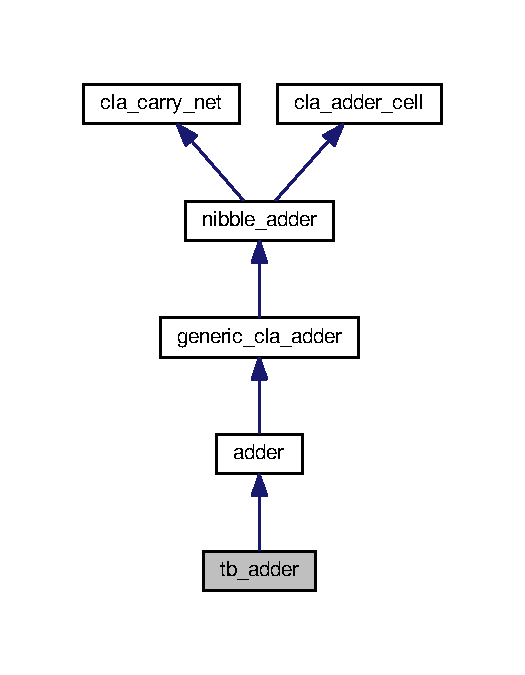
\includegraphics[width=252pt]{classtb__adder__inherit__graph}
\end{center}
\end{figure}


Diagramma di collaborazione per tb\+\_\+adder\+:
\nopagebreak
\begin{figure}[H]
\begin{center}
\leavevmode
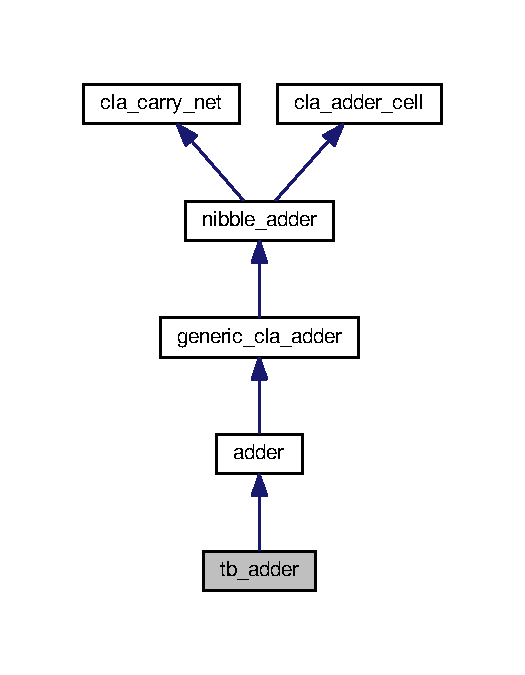
\includegraphics[width=252pt]{classtb__adder__coll__graph}
\end{center}
\end{figure}
\subsection*{Entities}
\begin{DoxyCompactItemize}
\item 
\hyperlink{classtb__adder_1_1behavior}{behavior} architecture
\end{DoxyCompactItemize}


La documentazione per questa classe è stata generata a partire dal seguente file\+:\begin{DoxyCompactItemize}
\item 
Src/adder/\hyperlink{tb__adder_8vhd}{tb\+\_\+adder.\+vhd}\end{DoxyCompactItemize}

\hypertarget{classtb__generic__cla__adder}{\section{tb\+\_\+generic\+\_\+cla\+\_\+adder Entity Reference}
\label{classtb__generic__cla__adder}\index{tb\+\_\+generic\+\_\+cla\+\_\+adder@{tb\+\_\+generic\+\_\+cla\+\_\+adder}}
}


Diagramma delle classi per tb\+\_\+generic\+\_\+cla\+\_\+adder\nopagebreak
\begin{figure}[H]
\begin{center}
\leavevmode
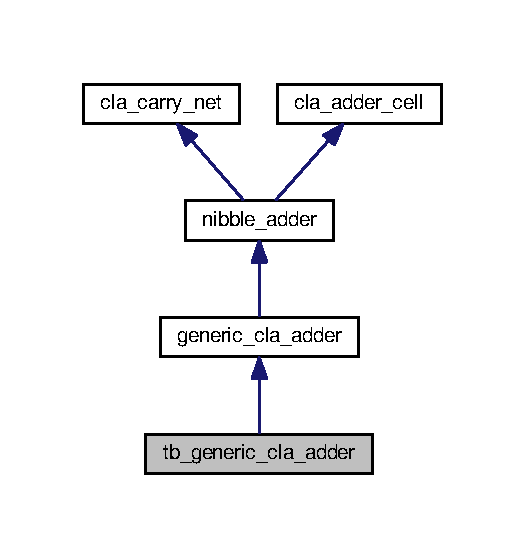
\includegraphics[width=252pt]{classtb__generic__cla__adder__inherit__graph}
\end{center}
\end{figure}


Diagramma di collaborazione per tb\+\_\+generic\+\_\+cla\+\_\+adder\+:\nopagebreak
\begin{figure}[H]
\begin{center}
\leavevmode
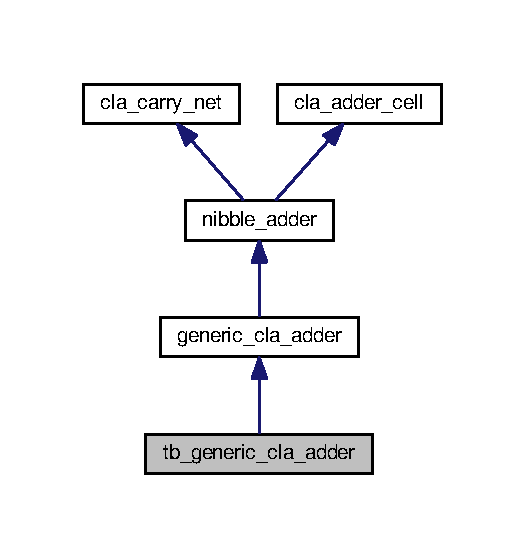
\includegraphics[width=252pt]{classtb__generic__cla__adder__coll__graph}
\end{center}
\end{figure}
\subsection*{Entities}
\begin{DoxyCompactItemize}
\item 
\hyperlink{classtb__generic__cla__adder_1_1behavior}{behavior} architecture
\end{DoxyCompactItemize}


La documentazione per questa classe è stata generata a partire dal seguente file\+:\begin{DoxyCompactItemize}
\item 
Src/adder/\hyperlink{tb__generic__cla__adder_8vhd}{tb\+\_\+generic\+\_\+cla\+\_\+adder.\+vhd}\end{DoxyCompactItemize}

\hypertarget{classtb___linear_regression}{}\section{tb\+\_\+\+Linear\+Regression Entity Reference}
\label{classtb___linear_regression}\index{tb\+\_\+\+Linear\+Regression@{tb\+\_\+\+Linear\+Regression}}


Diagramma delle classi per tb\+\_\+\+Linear\+Regression

\chapter{Documentazione dei file}
\hypertarget{adder_8vhd}{\section{Riferimenti per il file Src/adder/adder.vhd}
\label{adder_8vhd}\index{Src/adder/adder.\+vhd@{Src/adder/adder.\+vhd}}
}
\subsection*{Entities}
\begin{DoxyCompactItemize}
\item 
\hyperlink{classadder}{adder} entity
\item 
\hyperlink{classadder_1_1structural}{structural} architecture
\end{DoxyCompactItemize}


\subsection{Descrizione dettagliata}
\begin{DoxyAuthor}{Autori}
Salvatore Barone \href{mailto:salvator.barone@gmail.com}{\tt salvator.\+barone@gmail.\+com} ~\newline
 Alfonso Di Martino \href{mailto:alfonsodimartino160989@gmail.com}{\tt alfonsodimartino160989@gmail.\+com} ~\newline
 Sossio Fiorillo \href{mailto:fsossio@gmail.com}{\tt fsossio@gmail.\+com} ~\newline
 Pietro Liguori \href{mailto:pie.liguori@gmail.com}{\tt pie.\+liguori@gmail.\+com} ~\newline

\end{DoxyAuthor}
\begin{DoxyDate}{Data}
01 07 2017
\end{DoxyDate}
\begin{DoxyCopyright}{Copyright}
Copyright 2017 Salvatore Barone \href{mailto:salvator.barone@gmail.com}{\tt salvator.\+barone@gmail.\+com} ~\newline
 Alfonso Di Martino \href{mailto:alfonsodimartino160989@gmail.com}{\tt alfonsodimartino160989@gmail.\+com} ~\newline
 Sossio Fiorillo \href{mailto:fsossio@gmail.com}{\tt fsossio@gmail.\+com} ~\newline
 Pietro Liguori \href{mailto:pie.liguori@gmail.com}{\tt pie.\+liguori@gmail.\+com} ~\newline

\end{DoxyCopyright}
This file is part of Linear-\/\+Regression.

Linear-\/\+Regression is free software; you can redistribute it and/or modify it under the terms of the G\+N\+U General Public License as published by the Free Software Foundation; either version 3 of the License, or any later version.

Linear-\/\+Regression is distributed in the hope that it will be useful, but W\+I\+T\+H\+O\+U\+T A\+N\+Y W\+A\+R\+R\+A\+N\+T\+Y; without even the implied warranty of M\+E\+R\+C\+H\+A\+N\+T\+A\+B\+I\+L\+I\+T\+Y or F\+I\+T\+N\+E\+S\+S F\+O\+R A P\+A\+R\+T\+I\+C\+U\+L\+A\+R P\+U\+R\+P\+O\+S\+E. See the G\+N\+U General Public License for more details.

You should have received a copy of the G\+N\+U General Public License along with this program; if not, write to the Free Software Foundation, Inc., 51 Franklin Street, Fifth Floor, Boston, M\+A 02110-\/1301, U\+S\+A. 
\hypertarget{cla__adder__cell_8vhd}{\section{Riferimenti per il file Src/adder/cla\+\_\+adder\+\_\+cell.vhd}
\label{cla__adder__cell_8vhd}\index{Src/adder/cla\+\_\+adder\+\_\+cell.\+vhd@{Src/adder/cla\+\_\+adder\+\_\+cell.\+vhd}}
}
\subsection*{Entities}
\begin{DoxyCompactItemize}
\item 
\hyperlink{classcla__adder__cell}{cla\+\_\+adder\+\_\+cell} entity
\begin{DoxyCompactList}\small\item\em Cella base di un addizionatore con carry-\/lookahead.

La cella somma tra loro due addendi ed un carry in ingresso, tutti espressi su un solo bit. Oltre a generare la somma, genera le funzioni \char`\"{}propagazione\char`\"{} e \char`\"{}generazione\char`\"{} del carry. \end{DoxyCompactList}\item 
\hyperlink{classcla__adder__cell_1_1dataflow}{dataflow} architecture
\end{DoxyCompactItemize}


\subsection{Descrizione dettagliata}
\begin{DoxyAuthor}{Autori}
Salvatore Barone \href{mailto:salvator.barone@gmail.com}{\tt salvator.\+barone@gmail.\+com} ~\newline
 Alfonso Di Martino \href{mailto:alfonsodimartino160989@gmail.com}{\tt alfonsodimartino160989@gmail.\+com} ~\newline
 Sossio Fiorillo \href{mailto:fsossio@gmail.com}{\tt fsossio@gmail.\+com} ~\newline
 Pietro Liguori \href{mailto:pie.liguori@gmail.com}{\tt pie.\+liguori@gmail.\+com} ~\newline

\end{DoxyAuthor}
\begin{DoxyDate}{Data}
01 07 2017
\end{DoxyDate}
\begin{DoxyCopyright}{Copyright}
Copyright 2017 Salvatore Barone \href{mailto:salvator.barone@gmail.com}{\tt salvator.\+barone@gmail.\+com} ~\newline
 Alfonso Di Martino \href{mailto:alfonsodimartino160989@gmail.com}{\tt alfonsodimartino160989@gmail.\+com} ~\newline
 Sossio Fiorillo \href{mailto:fsossio@gmail.com}{\tt fsossio@gmail.\+com} ~\newline
 Pietro Liguori \href{mailto:pie.liguori@gmail.com}{\tt pie.\+liguori@gmail.\+com} ~\newline

\end{DoxyCopyright}
This file is part of Linear-\/\+Regression.

Linear-\/\+Regression is free software; you can redistribute it and/or modify it under the terms of the G\+N\+U General Public License as published by the Free Software Foundation; either version 3 of the License, or any later version.

Linear-\/\+Regression is distributed in the hope that it will be useful, but W\+I\+T\+H\+O\+U\+T A\+N\+Y W\+A\+R\+R\+A\+N\+T\+Y; without even the implied warranty of M\+E\+R\+C\+H\+A\+N\+T\+A\+B\+I\+L\+I\+T\+Y or F\+I\+T\+N\+E\+S\+S F\+O\+R A P\+A\+R\+T\+I\+C\+U\+L\+A\+R P\+U\+R\+P\+O\+S\+E. See the G\+N\+U General Public License for more details.

You should have received a copy of the G\+N\+U General Public License along with this program; if not, write to the Free Software Foundation, Inc., 51 Franklin Street, Fifth Floor, Boston, M\+A 02110-\/1301, U\+S\+A. 
\hypertarget{cla__carry__net_8vhd}{\section{Riferimenti per il file Src/adder/cla\+\_\+carry\+\_\+net.vhd}
\label{cla__carry__net_8vhd}\index{Src/adder/cla\+\_\+carry\+\_\+net.\+vhd@{Src/adder/cla\+\_\+carry\+\_\+net.\+vhd}}
}
\subsection*{Entities}
\begin{DoxyCompactItemize}
\item 
\hyperlink{classcla__carry__net}{cla\+\_\+carry\+\_\+net} entity
\begin{DoxyCompactList}\small\item\em Rete logica di calcolo dei riporti per un addizionatore a quattro bit con carry lookahead.

Permette di anticipare il calcolo dei riporti usando le funzioni \char`\"{}propagazione\char`\"{} e \char`\"{}generazione\char`\"{} prodotte dai singoli blocchi \hyperlink{classcla__adder__cell}{cla\+\_\+adder\+\_\+cell}, in modo da ridurre tempo necessario ad effettuare il calcolo di tutti i carry, quindi il tempo necessario a completare la somma. Questo blocco calcola solo i carry, pertanto va connesso ai blocchi \hyperlink{classcla__adder__cell}{cla\+\_\+adder\+\_\+cell}, per il calcolo materiale della somma, così come indicato dallo schema seguente, il quale rappresenta lo schema completo di un addizionatore a quattro bit\+: . \end{DoxyCompactList}\item 
\hyperlink{classcla__carry__net_1_1dataflow}{dataflow} architecture
\begin{DoxyCompactList}\small\item\em Implementazione dataflow dell'entita' \hyperlink{classcla__carry__net}{cla\+\_\+carry\+\_\+net}. \end{DoxyCompactList}\end{DoxyCompactItemize}


\subsection{Descrizione dettagliata}
\begin{DoxyAuthor}{Autori}
Salvatore Barone \href{mailto:salvator.barone@gmail.com}{\tt salvator.\+barone@gmail.\+com} ~\newline
 Alfonso Di Martino \href{mailto:alfonsodimartino160989@gmail.com}{\tt alfonsodimartino160989@gmail.\+com} ~\newline
 Sossio Fiorillo \href{mailto:fsossio@gmail.com}{\tt fsossio@gmail.\+com} ~\newline
 Pietro Liguori \href{mailto:pie.liguori@gmail.com}{\tt pie.\+liguori@gmail.\+com} ~\newline

\end{DoxyAuthor}
\begin{DoxyDate}{Data}
01 07 2017
\end{DoxyDate}
\begin{DoxyCopyright}{Copyright}
Copyright 2017 Salvatore Barone \href{mailto:salvator.barone@gmail.com}{\tt salvator.\+barone@gmail.\+com} ~\newline
 Alfonso Di Martino \href{mailto:alfonsodimartino160989@gmail.com}{\tt alfonsodimartino160989@gmail.\+com} ~\newline
 Sossio Fiorillo \href{mailto:fsossio@gmail.com}{\tt fsossio@gmail.\+com} ~\newline
 Pietro Liguori \href{mailto:pie.liguori@gmail.com}{\tt pie.\+liguori@gmail.\+com} ~\newline

\end{DoxyCopyright}
This file is part of Linear-\/\+Regression.

Linear-\/\+Regression is free software; you can redistribute it and/or modify it under the terms of the G\+N\+U General Public License as published by the Free Software Foundation; either version 3 of the License, or any later version.

Linear-\/\+Regression is distributed in the hope that it will be useful, but W\+I\+T\+H\+O\+U\+T A\+N\+Y W\+A\+R\+R\+A\+N\+T\+Y; without even the implied warranty of M\+E\+R\+C\+H\+A\+N\+T\+A\+B\+I\+L\+I\+T\+Y or F\+I\+T\+N\+E\+S\+S F\+O\+R A P\+A\+R\+T\+I\+C\+U\+L\+A\+R P\+U\+R\+P\+O\+S\+E. See the G\+N\+U General Public License for more details.

You should have received a copy of the G\+N\+U General Public License along with this program; if not, write to the Free Software Foundation, Inc., 51 Franklin Street, Fifth Floor, Boston, M\+A 02110-\/1301, U\+S\+A. 
\hypertarget{generic__cla__adder_8vhd}{\section{Riferimenti per il file Src/adder/generic\+\_\+cla\+\_\+adder.vhd}
\label{generic__cla__adder_8vhd}\index{Src/adder/generic\+\_\+cla\+\_\+adder.\+vhd@{Src/adder/generic\+\_\+cla\+\_\+adder.\+vhd}}
}
\subsection*{Entities}
\begin{DoxyCompactItemize}
\item 
\hyperlink{classgeneric__cla__adder}{generic\+\_\+cla\+\_\+adder} entity
\begin{DoxyCompactList}\small\item\em Adder custom con carry-\/lookahead

\hyperlink{classgeneric__cla__adder}{generic\+\_\+cla\+\_\+adder} somma tra loro due addendi ed un carry in ingresso; gli addendi sono espressi su multipli interi di quattro bit. Oltre a generare la somma, genera il flag di carry ed il flag di overflow. \end{DoxyCompactList}\item 
\hyperlink{classgeneric__cla__adder_1_1structural}{structural} architecture
\begin{DoxyCompactList}\small\item\em Implementazione structural di \hyperlink{classgeneric__cla__adder}{generic\+\_\+cla\+\_\+adder}. \end{DoxyCompactList}\end{DoxyCompactItemize}


\subsection{Descrizione dettagliata}
\begin{DoxyAuthor}{Autori}
Salvatore Barone \href{mailto:salvator.barone@gmail.com}{\tt salvator.\+barone@gmail.\+com} ~\newline
 Alfonso Di Martino \href{mailto:alfonsodimartino160989@gmail.com}{\tt alfonsodimartino160989@gmail.\+com} ~\newline
 Sossio Fiorillo \href{mailto:fsossio@gmail.com}{\tt fsossio@gmail.\+com} ~\newline
 Pietro Liguori \href{mailto:pie.liguori@gmail.com}{\tt pie.\+liguori@gmail.\+com} ~\newline

\end{DoxyAuthor}
\begin{DoxyDate}{Data}
01 07 2017
\end{DoxyDate}
\begin{DoxyCopyright}{Copyright}
Copyright 2017 Salvatore Barone \href{mailto:salvator.barone@gmail.com}{\tt salvator.\+barone@gmail.\+com} ~\newline
 Alfonso Di Martino \href{mailto:alfonsodimartino160989@gmail.com}{\tt alfonsodimartino160989@gmail.\+com} ~\newline
 Sossio Fiorillo \href{mailto:fsossio@gmail.com}{\tt fsossio@gmail.\+com} ~\newline
 Pietro Liguori \href{mailto:pie.liguori@gmail.com}{\tt pie.\+liguori@gmail.\+com} ~\newline

\end{DoxyCopyright}
This file is part of Linear-\/\+Regression.

Linear-\/\+Regression is free software; you can redistribute it and/or modify it under the terms of the G\+N\+U General Public License as published by the Free Software Foundation; either version 3 of the License, or any later version.

Linear-\/\+Regression is distributed in the hope that it will be useful, but W\+I\+T\+H\+O\+U\+T A\+N\+Y W\+A\+R\+R\+A\+N\+T\+Y; without even the implied warranty of M\+E\+R\+C\+H\+A\+N\+T\+A\+B\+I\+L\+I\+T\+Y or F\+I\+T\+N\+E\+S\+S F\+O\+R A P\+A\+R\+T\+I\+C\+U\+L\+A\+R P\+U\+R\+P\+O\+S\+E. See the G\+N\+U General Public License for more details.

You should have received a copy of the G\+N\+U General Public License along with this program; if not, write to the Free Software Foundation, Inc., 51 Franklin Street, Fifth Floor, Boston, M\+A 02110-\/1301, U\+S\+A. 
\hypertarget{nibble__adder_8vhd}{}\section{Riferimenti per il file Src/adder/nibble\+\_\+adder.vhd}
\label{nibble__adder_8vhd}\index{Src/adder/nibble\+\_\+adder.\+vhd@{Src/adder/nibble\+\_\+adder.\+vhd}}
\subsection*{Entities}
\begin{DoxyCompactItemize}
\item 
\hyperlink{classnibble__adder}{nibble\+\_\+adder} entity
\begin{DoxyCompactList}\small\item\em Addizionatore con carry-\/lookahead a quattro bit.

La cella somma tra loro due addendi ed un carry in ingresso; gli addendi sono espressi su quattro bit. Oltre a generare la somma, genera le funzioni \char`\"{}propagazione\char`\"{} e \char`\"{}generazione\char`\"{} del carry per eventuali blocchi \hyperlink{classnibble__adder}{nibble\+\_\+adder} posti a valle. \end{DoxyCompactList}\item 
\hyperlink{classnibble__adder_1_1structural}{structural} architecture
\begin{DoxyCompactList}\small\item\em Implementazione structural dell\textquotesingle{}entità \hyperlink{classnibble__adder}{nibble\+\_\+adder}.

Questa architettura istanzia una entità \hyperlink{classcla__carry__net}{cla\+\_\+carry\+\_\+net} ed una entità \hyperlink{classcla__adder__cell}{cla\+\_\+adder\+\_\+cell} per ogni bit su cui sono espressi gli addendi, connettendoli tra loro secondo lo schema riportato di seguito\+: . \end{DoxyCompactList}\end{DoxyCompactItemize}


\subsection{Descrizione dettagliata}
\begin{DoxyAuthor}{Autori}
Salvatore Barone \href{mailto:salvator.barone@gmail.com}{\tt salvator.\+barone@gmail.\+com} ~\newline
 Alfonso Di Martino \href{mailto:alfonsodimartino160989@gmail.com}{\tt alfonsodimartino160989@gmail.\+com} ~\newline
 Sossio Fiorillo \href{mailto:fsossio@gmail.com}{\tt fsossio@gmail.\+com} ~\newline
 Pietro Liguori \href{mailto:pie.liguori@gmail.com}{\tt pie.\+liguori@gmail.\+com} ~\newline

\end{DoxyAuthor}
\begin{DoxyDate}{Data}
01 07 2017
\end{DoxyDate}
\begin{DoxyCopyright}{Copyright}
Copyright 2017 Salvatore Barone \href{mailto:salvator.barone@gmail.com}{\tt salvator.\+barone@gmail.\+com} ~\newline
 Alfonso Di Martino \href{mailto:alfonsodimartino160989@gmail.com}{\tt alfonsodimartino160989@gmail.\+com} ~\newline
 Sossio Fiorillo \href{mailto:fsossio@gmail.com}{\tt fsossio@gmail.\+com} ~\newline
 Pietro Liguori \href{mailto:pie.liguori@gmail.com}{\tt pie.\+liguori@gmail.\+com} ~\newline

\end{DoxyCopyright}
This file is part of Linear-\/\+Regression.

Linear-\/\+Regression is free software; you can redistribute it and/or modify it under the terms of the G\+NU General Public License as published by the Free Software Foundation; either version 3 of the License, or any later version.

Linear-\/\+Regression is distributed in the hope that it will be useful, but W\+I\+T\+H\+O\+UT A\+NY W\+A\+R\+R\+A\+N\+TY; without even the implied warranty of M\+E\+R\+C\+H\+A\+N\+T\+A\+B\+I\+L\+I\+TY or F\+I\+T\+N\+E\+SS F\+OR A P\+A\+R\+T\+I\+C\+U\+L\+AR P\+U\+R\+P\+O\+SE. See the G\+NU General Public License for more details.

You should have received a copy of the G\+NU General Public License along with this program; if not, write to the Free Software Foundation, Inc., 51 Franklin Street, Fifth Floor, Boston, MA 02110-\/1301, U\+SA. 
\hypertarget{tb__adder_8vhd}{}\section{Riferimenti per il file Src/adder/tb\+\_\+adder.vhd}
\label{tb__adder_8vhd}\index{Src/adder/tb\+\_\+adder.\+vhd@{Src/adder/tb\+\_\+adder.\+vhd}}
\subsection*{Entities}
\begin{DoxyCompactItemize}
\item 
\hyperlink{classtb__adder}{tb\+\_\+adder} entity
\item 
\hyperlink{classtb__adder_1_1behavior}{behavior} architecture
\end{DoxyCompactItemize}


\subsection{Descrizione dettagliata}
\begin{DoxyAuthor}{Autori}
Salvatore Barone \href{mailto:salvator.barone@gmail.com}{\tt salvator.\+barone@gmail.\+com} ~\newline
 Alfonso Di Martino \href{mailto:alfonsodimartino160989@gmail.com}{\tt alfonsodimartino160989@gmail.\+com} ~\newline
 Sossio Fiorillo \href{mailto:fsossio@gmail.com}{\tt fsossio@gmail.\+com} ~\newline
 Pietro Liguori \href{mailto:pie.liguori@gmail.com}{\tt pie.\+liguori@gmail.\+com} ~\newline

\end{DoxyAuthor}
\begin{DoxyDate}{Data}
01 07 2017
\end{DoxyDate}
\begin{DoxyCopyright}{Copyright}
Copyright 2017 Salvatore Barone \href{mailto:salvator.barone@gmail.com}{\tt salvator.\+barone@gmail.\+com} ~\newline
 Alfonso Di Martino \href{mailto:alfonsodimartino160989@gmail.com}{\tt alfonsodimartino160989@gmail.\+com} ~\newline
 Sossio Fiorillo \href{mailto:fsossio@gmail.com}{\tt fsossio@gmail.\+com} ~\newline
 Pietro Liguori \href{mailto:pie.liguori@gmail.com}{\tt pie.\+liguori@gmail.\+com} ~\newline

\end{DoxyCopyright}
This file is part of Linear-\/\+Regression.

Linear-\/\+Regression is free software; you can redistribute it and/or modify it under the terms of the G\+NU General Public License as published by the Free Software Foundation; either version 3 of the License, or any later version.

Linear-\/\+Regression is distributed in the hope that it will be useful, but W\+I\+T\+H\+O\+UT A\+NY W\+A\+R\+R\+A\+N\+TY; without even the implied warranty of M\+E\+R\+C\+H\+A\+N\+T\+A\+B\+I\+L\+I\+TY or F\+I\+T\+N\+E\+SS F\+OR A P\+A\+R\+T\+I\+C\+U\+L\+AR P\+U\+R\+P\+O\+SE. See the G\+NU General Public License for more details.

You should have received a copy of the G\+NU General Public License along with this program; if not, write to the Free Software Foundation, Inc., 51 Franklin Street, Fifth Floor, Boston, MA 02110-\/1301, U\+SA. 
\hypertarget{tb__generic__cla__adder_8vhd}{}\section{Riferimenti per il file Src/adder/tb\+\_\+generic\+\_\+cla\+\_\+adder.vhd}
\label{tb__generic__cla__adder_8vhd}\index{Src/adder/tb\+\_\+generic\+\_\+cla\+\_\+adder.\+vhd@{Src/adder/tb\+\_\+generic\+\_\+cla\+\_\+adder.\+vhd}}
\subsection*{Entities}
\begin{DoxyCompactItemize}
\item 
\hyperlink{classtb__generic__cla__adder}{tb\+\_\+generic\+\_\+cla\+\_\+adder} entity
\item 
\hyperlink{classtb__generic__cla__adder_1_1behavior}{behavior} architecture
\end{DoxyCompactItemize}


\subsection{Descrizione dettagliata}
\begin{DoxyAuthor}{Autori}
Salvatore Barone \href{mailto:salvator.barone@gmail.com}{\tt salvator.\+barone@gmail.\+com} ~\newline
 Alfonso Di Martino \href{mailto:alfonsodimartino160989@gmail.com}{\tt alfonsodimartino160989@gmail.\+com} ~\newline
 Sossio Fiorillo \href{mailto:fsossio@gmail.com}{\tt fsossio@gmail.\+com} ~\newline
 Pietro Liguori \href{mailto:pie.liguori@gmail.com}{\tt pie.\+liguori@gmail.\+com} ~\newline

\end{DoxyAuthor}
\begin{DoxyDate}{Data}
01 07 2017
\end{DoxyDate}
\begin{DoxyCopyright}{Copyright}
Copyright 2017 Salvatore Barone \href{mailto:salvator.barone@gmail.com}{\tt salvator.\+barone@gmail.\+com} ~\newline
 Alfonso Di Martino \href{mailto:alfonsodimartino160989@gmail.com}{\tt alfonsodimartino160989@gmail.\+com} ~\newline
 Sossio Fiorillo \href{mailto:fsossio@gmail.com}{\tt fsossio@gmail.\+com} ~\newline
 Pietro Liguori \href{mailto:pie.liguori@gmail.com}{\tt pie.\+liguori@gmail.\+com} ~\newline

\end{DoxyCopyright}
This file is part of Linear-\/\+Regression.

Linear-\/\+Regression is free software; you can redistribute it and/or modify it under the terms of the G\+NU General Public License as published by the Free Software Foundation; either version 3 of the License, or any later version.

Linear-\/\+Regression is distributed in the hope that it will be useful, but W\+I\+T\+H\+O\+UT A\+NY W\+A\+R\+R\+A\+N\+TY; without even the implied warranty of M\+E\+R\+C\+H\+A\+N\+T\+A\+B\+I\+L\+I\+TY or F\+I\+T\+N\+E\+SS F\+OR A P\+A\+R\+T\+I\+C\+U\+L\+AR P\+U\+R\+P\+O\+SE. See the G\+NU General Public License for more details.

You should have received a copy of the G\+NU General Public License along with this program; if not, write to the Free Software Foundation, Inc., 51 Franklin Street, Fifth Floor, Boston, MA 02110-\/1301, U\+SA. 
\hypertarget{_linear_regression_8vhd}{\section{Riferimenti per il file Src/\+Linear\+Regression.vhd}
\label{_linear_regression_8vhd}\index{Src/\+Linear\+Regression.\+vhd@{Src/\+Linear\+Regression.\+vhd}}
}
\subsection*{Entities}
\begin{DoxyCompactItemize}
\item 
\hyperlink{class_linear_regression}{Linear\+Regression} entity
\item 
\hyperlink{class_linear_regression_1_1_structural}{Structural} architecture
\begin{DoxyCompactList}\small\item\em Per il calcolo dei parametri della regressione vengono utilizzati opportunamente dei moltiplicatori e addizionatori/sottrattori. Per effettuare i calcoli in fixed point vengono adoperati opportuni troncamenti/ espansioni dei segnali. Il componente ha un'architettura pipelined, così come mostrato nello schema di seguito, nel quale sono indicati, usando la notazione standard, le rappresentazioni binarie dei segnali dato in signed fixed-\/point. Si noti che il segnale \char`\"{}load\char`\"{} agisce solo sul primo dei registri della pipe. . \end{DoxyCompactList}\end{DoxyCompactItemize}


\subsection{Descrizione dettagliata}
\begin{DoxyAuthor}{Autori}
Salvatore Barone \href{mailto:salvator.barone@gmail.com}{\tt salvator.\+barone@gmail.\+com} ~\newline
 Alfonso Di Martino \href{mailto:alfonsodimartino160989@gmail.com}{\tt alfonsodimartino160989@gmail.\+com} ~\newline
 Sossio Fiorillo \href{mailto:fsossio@gmail.com}{\tt fsossio@gmail.\+com} ~\newline
 Pietro Liguori \href{mailto:pie.liguori@gmail.com}{\tt pie.\+liguori@gmail.\+com} ~\newline

\end{DoxyAuthor}
\begin{DoxyDate}{Data}
03 07 2017
\end{DoxyDate}
\begin{DoxyCopyright}{Copyright}
Copyright 2017 Salvatore Barone \href{mailto:salvator.barone@gmail.com}{\tt salvator.\+barone@gmail.\+com} ~\newline
 Alfonso Di Martino \href{mailto:alfonsodimartino160989@gmail.com}{\tt alfonsodimartino160989@gmail.\+com} ~\newline
 Sossio Fiorillo \href{mailto:fsossio@gmail.com}{\tt fsossio@gmail.\+com} ~\newline
 Pietro Liguori \href{mailto:pie.liguori@gmail.com}{\tt pie.\+liguori@gmail.\+com} ~\newline

\end{DoxyCopyright}
This file is part of Linear-\/\+Regression.

Linear-\/\+Regression is free software; you can redistribute it and/or modify it under the terms of the G\+N\+U General Public License as published by the Free Software Foundation; either version 3 of the License, or any later version.

Linear-\/\+Regression is distributed in the hope that it will be useful, but W\+I\+T\+H\+O\+U\+T A\+N\+Y W\+A\+R\+R\+A\+N\+T\+Y; without even the implied warranty of M\+E\+R\+C\+H\+A\+N\+T\+A\+B\+I\+L\+I\+T\+Y or F\+I\+T\+N\+E\+S\+S F\+O\+R A P\+A\+R\+T\+I\+C\+U\+L\+A\+R P\+U\+R\+P\+O\+S\+E. See the G\+N\+U General Public License for more details.

You should have received a copy of the G\+N\+U General Public License along with this program; if not, write to the Free Software Foundation, Inc., 51 Franklin Street, Fifth Floor, Boston, M\+A 02110-\/1301, U\+S\+A. 
\hypertarget{multiplier_8vhd}{\section{Riferimenti per il file Src/multiplier.vhd}
\label{multiplier_8vhd}\index{Src/multiplier.\+vhd@{Src/multiplier.\+vhd}}
}
\subsection*{Entities}
\begin{DoxyCompactItemize}
\item 
\hyperlink{classmultiplier}{multiplier} entity
\begin{DoxyCompactList}\small\item\em Moltiplicatore a due fattori. \end{DoxyCompactList}\item 
\hyperlink{classmultiplier_1_1_structural}{Structural} architecture
\begin{DoxyCompactList}\small\item\em Per il prodotto viene utilizzato l'operatore $\ast$. La sintesi viene lasciata al particolare sintetizzatore. \end{DoxyCompactList}\end{DoxyCompactItemize}


\subsection{Descrizione dettagliata}
\begin{DoxyAuthor}{Autori}
Salvatore Barone \href{mailto:salvator.barone@gmail.com}{\tt salvator.\+barone@gmail.\+com} ~\newline
 Alfonso Di Martino \href{mailto:alfonsodimartino160989@gmail.com}{\tt alfonsodimartino160989@gmail.\+com} ~\newline
 Sossio Fiorillo \href{mailto:fsossio@gmail.com}{\tt fsossio@gmail.\+com} ~\newline
 Pietro Liguori \href{mailto:pie.liguori@gmail.com}{\tt pie.\+liguori@gmail.\+com} ~\newline

\end{DoxyAuthor}
\begin{DoxyDate}{Data}
03 07 2017
\end{DoxyDate}
\begin{DoxyCopyright}{Copyright}
Copyright 2017 Salvatore Barone \href{mailto:salvator.barone@gmail.com}{\tt salvator.\+barone@gmail.\+com} ~\newline
 Alfonso Di Martino \href{mailto:alfonsodimartino160989@gmail.com}{\tt alfonsodimartino160989@gmail.\+com} ~\newline
 Sossio Fiorillo \href{mailto:fsossio@gmail.com}{\tt fsossio@gmail.\+com} ~\newline
 Pietro Liguori \href{mailto:pie.liguori@gmail.com}{\tt pie.\+liguori@gmail.\+com} ~\newline

\end{DoxyCopyright}
This file is part of Linear-\/\+Regression.

Linear-\/\+Regression is free software; you can redistribute it and/or modify it under the terms of the G\+N\+U General Public License as published by the Free Software Foundation; either version 3 of the License, or any later version.

Linear-\/\+Regression is distributed in the hope that it will be useful, but W\+I\+T\+H\+O\+U\+T A\+N\+Y W\+A\+R\+R\+A\+N\+T\+Y; without even the implied warranty of M\+E\+R\+C\+H\+A\+N\+T\+A\+B\+I\+L\+I\+T\+Y or F\+I\+T\+N\+E\+S\+S F\+O\+R A P\+A\+R\+T\+I\+C\+U\+L\+A\+R P\+U\+R\+P\+O\+S\+E. See the G\+N\+U General Public License for more details.

You should have received a copy of the G\+N\+U General Public License along with this program; if not, write to the Free Software Foundation, Inc., 51 Franklin Street, Fifth Floor, Boston, M\+A 02110-\/1301, U\+S\+A. 
\hypertarget{tb___linear_regression_8vhd}{}\section{Riferimenti per il file Src/tb\+\_\+\+Linear\+Regression.vhd}
\label{tb___linear_regression_8vhd}\index{Src/tb\+\_\+\+Linear\+Regression.\+vhd@{Src/tb\+\_\+\+Linear\+Regression.\+vhd}}
\subsection*{Entities}
\begin{DoxyCompactItemize}
\item 
\hyperlink{classtb___linear_regression}{tb\+\_\+\+Linear\+Regression} entity
\item 
\hyperlink{classtb___linear_regression_1_1_behavioral}{Behavioral} architecture
\end{DoxyCompactItemize}


\subsection{Descrizione dettagliata}
\begin{DoxyAuthor}{Autori}
Salvatore Barone \href{mailto:salvator.barone@gmail.com}{\tt salvator.\+barone@gmail.\+com} ~\newline
 Alfonso Di Martino \href{mailto:alfonsodimartino160989@gmail.com}{\tt alfonsodimartino160989@gmail.\+com} ~\newline
 Sossio Fiorillo \href{mailto:fsossio@gmail.com}{\tt fsossio@gmail.\+com} ~\newline
 Pietro Liguori \href{mailto:pie.liguori@gmail.com}{\tt pie.\+liguori@gmail.\+com} ~\newline

\end{DoxyAuthor}
\begin{DoxyDate}{Data}
03 07 2017
\end{DoxyDate}
\begin{DoxyCopyright}{Copyright}
Copyright 2017 Salvatore Barone \href{mailto:salvator.barone@gmail.com}{\tt salvator.\+barone@gmail.\+com} ~\newline
 Alfonso Di Martino \href{mailto:alfonsodimartino160989@gmail.com}{\tt alfonsodimartino160989@gmail.\+com} ~\newline
 Sossio Fiorillo \href{mailto:fsossio@gmail.com}{\tt fsossio@gmail.\+com} ~\newline
 Pietro Liguori \href{mailto:pie.liguori@gmail.com}{\tt pie.\+liguori@gmail.\+com} ~\newline

\end{DoxyCopyright}
This file is part of Linear-\/\+Regression.

Linear-\/\+Regression is free software; you can redistribute it and/or modify it under the terms of the G\+NU General Public License as published by the Free Software Foundation; either version 3 of the License, or any later version.

Linear-\/\+Regression is distributed in the hope that it will be useful, but W\+I\+T\+H\+O\+UT A\+NY W\+A\+R\+R\+A\+N\+TY; without even the implied warranty of M\+E\+R\+C\+H\+A\+N\+T\+A\+B\+I\+L\+I\+TY or F\+I\+T\+N\+E\+SS F\+OR A P\+A\+R\+T\+I\+C\+U\+L\+AR P\+U\+R\+P\+O\+SE. See the G\+NU General Public License for more details.

You should have received a copy of the G\+NU General Public License along with this program; if not, write to the Free Software Foundation, Inc., 51 Franklin Street, Fifth Floor, Boston, MA 02110-\/1301, U\+SA. 
%--- End generated contents ---

% Index
\backmatter
\newpage
\phantomsection
\clearemptydoublepage
\addcontentsline{toc}{chapter}{Indice}
\printindex

\end{document}
